%このファイルをコンパイルする。

\documentclass[10pt,a4j,dvipdfmx,openany,uplatex]{jsbook}

\setcounter{secnumdepth}{3}%\subsubsectionのタイトルを表示するときは3にする。

%パッケージ

\usepackage[dvipdfmx]{graphicx, xcolor}
\usepackage{picture}%図とか
\usepackage{ulem}
\usepackage[labelformat=empty]{subcaption}
\usepackage{caption}%キャプションの番号消し
\usepackage{multirow}%複雑な表のために
%--------------------------------------------------
\usepackage{xparse}

\usepackage[top=30truemm, bottom=25truemm, left=20truemm, right=20truemm]{geometry}

\usepackage[stable]{footmisc}%章節などの見出しの中で注を使う
\usepackage{uline--}%行分割可能な下線、ハイライト。ただし、TeXLive等に入ってはいないので、uline--.styを作業ディレクトリに入れておくこと。

\usepackage{epigraph}
\setlength{\epigraphwidth}{.6\textwidth}
%エピグラフを表示するため。タバコの話で使用。

\usepackage{amsmath} %%数式。多分使わん。
\usepackage{amssymb} %%数式で出てくる特殊記号を使いたい人がいるかも

\usepackage{tikz} %%図の描画。念の為
\usetikzlibrary{arrows, chains, positioning, quotes,shapes} %shapes.geometric, shapes.misc}
\usetikzlibrary{shapes.gates.logic.US}
\usepackage{url} %%URLを貼る。texでは$%&@とかの特殊記号を書くのが面倒なので
\usepackage{float}
\usepackage{wrapfig} %%この2つは図の配置のため
%\usepackage{picinpar}%%図の配置。figwindow環境
\usepackage{floatflt}
\usepackage{pxrubrica} %%ルビが打てます。
\usepackage{otf} %%珍しい文字を使いたい人のために。ほとんどの文字はuplatexの機能として、そのまま組めるので基本は使わなくてもいいと思う


\usepackage{multicol} \setlength{\columnseprule}{0.4pt}%2段組のため(座談会とか)


\usepackage{fancybox}%itembox, shadebox, あと何かしらの箱
\usepackage{tcolorbox}%色付きの箱. tcolorboxじゃないとページをまたげないことに注意。
	\tcbuselibrary{breakable} %これがないとtcolorboxがページをまたげないので
  \tcbuselibrary{skins}
\usepackage{ascmac}




%%%%%%%%%%%%%%%%2段組の中で図を使うため
\makeatletter
\newenvironment{tablehere}
  {\def\@captype{table}}
  {}

\newenvironment{figurehere}
  {\def\@captype{figure}}
  {}
\makeatother
%%%%% \begin{figure}[h]の代りに、\begin{figurehere}とせよ


%%%%%%%%%%%%%%%%%%%章の体裁を変更する。
 \usepackage[explicit]{titlesec}%題名や章, 節の見出しの体裁を変える
\titleformat{\chapter}[display]{\bfseries\gtfamily}{}{10pt}{%
  \begin{tcolorbox}[%
    enhanced,%
    colback=white,colbacktitle=white,colframe=black,coltitle=black,%
    boxrule=1.5pt,sharp corners,%
    borderline={1.5pt}{3pt}{black},%
    ]%
    \centering 第\thechapter 章\\
    \LARGE #1%
  \end{tcolorbox}%
}
\titlespacing*{\chapter}{1pt}{-20pt}{1pt}[3pt]%章の上の空隙を0にする。

\titleformat{\section}[block]
  {}
  {\Large\bfseries\gtfamily #1}
  {10pt}
  {\titleline[l]{\titlerule*[5pt]{\tiny\textbullet}}\vspace{-20pt}}

\titleformat{\subsection}[block]{}
  {\large\bfseries\gtfamily ○#1}{10pt}{}
  {\vspace{-20pt}}

\titleformat{\subsubsection}[block]{}
  {〜{\bfseries\gtfamily#1}〜}{10pt}{}
  {}


\newcommand{\subsecdefault}{\input{subsecdefault.tex}}
\newcommand{\subsecnomaru}{\input{subsecmarunasi.tex}}
%\subsectionの仕様を変更する。\subsecnomaruで◯をなくす。\subsecdefaultで元に戻す。
\newcommand{\sectionnotitle}{\input{sectionnotitle.tex}}
\newcommand{\sectiondefault}{\input{sectiondefault.tex}}

%%マクロ
%%%%%%%%%%%%%%%%%%%%%%%%%%%%%%%%%%%%%%%%%%%%%%%%%%
\newcommand{\singo}[1]{{\textgt{#1}}}%全体。新語に。
\newcommand{\komoku}[1]{\noindent{〈\textbf{#1}〉}}%募集要項で使用。
\newcommand{\kkomoku}[1]{\vspace{3mm}\noindent{\textbf{《#1》}}}%項目2。女子寮生窓口で使用。
\newcommand{\kkkomoku}[2]{\vspace{1mm}\noindent \textbf{#1 #2}\\}%項目3。C12座談会の部屋紹介で使用。


\newcommand{\tatespace}{\vspace{1cm}}
\newcommand{\emphbf}[1]{\textgt{#1}}%強調として太字を使用している箇所
\newcommand{\bunsekisha}[2]{\vspace{-2mm}\rightline{{\small(#1:#2)}}}%文責について\bunsekisha{文責}{奥山田}で(文責:奥山田)が小さく右寄で表示。「文責」の箇所は「編集」とか「文字起こし」とかにすればいいかな。

%%%%%%%%%%%%%%%座談会関係のマクロ
\newcommand{\jinbutu}[1]{\vspace{2mm}\noindent #1\\}%座談会の人物紹介。C12座談会で使用した形式
\newcommand{\situmon}{\item[---------]}%インタビュー形式のもので、インタビュアーに使う。
\newcommand{\togaki}[1]{\vspace{1mm} \quad #1 \vspace{1mm}}%ト書き
\newcommand{\hang}[1]{\settowidth{\hangindent}{#1} #1}%1回生座談会人物紹介で使用。
\newcommand{\talker}[1]{\noindent{\gtfamily\bfseries #1}:}%座談会で喋っている人を示す命令。想定している書式は
%\talker{人}喋ったこと<改行×2>
%\talker{次の話者}喋ったこと
\newcommand{\talkerb}[1]{{\gtfamily\bfseries #1}:}%行頭以外で使いたい時
\newcommand{\talkpare}[1]{\noindent (#1)}%座談会中の(から始まる段落に使用。カッコの後ろのコメントアウト

%%%%%%%%%%%%%%\zenkakuspace{n}でn個の全角空白を出力する。wrapfigureの位置調整に必要。
\newcount\kaisu
\def\zenkakuspace#1{
  \kaisu = 0 \loop\ifnum\kaisu<#1
   
  \advance\kaisu by1\repeat
}




\newcommand{\hanten}[1]{\uline[background,color=black,width=1zw,position=.38zw]{\color{white}{\textbf{#1}}}}
%文字の白黒反転する。kyoto scienceの記事をに使用。\ctextはsoulパッケージで使えるようになる

\def\sshatai#1{\makebox[2.25zw][l]{\vphantom{#1}\rotatebox{-48.8}{\scalebox{0.875}[1.143]{\rotatebox{41.2}{\smash{\rlap{#1}}}}}}} %和文斜体を行うためのマクロ。改行に対応できない。

\newcounter{footnote1}%これらは、minipageの中で脚注をつけるために(結構めんどうなことをしています。)1day.texにて
\newcounter{footnote2}

%%%%%%%%%索引の設定
\usepackage{makeidx}
\makeindex%idxファイルを作れという命令
\renewcommand{\seename}{$\Longrightarrow$}
\newcommand{\also}{$\longrightarrow$}
%「を見よ参照」を二重矢印、「をも見よ参照」を矢印に。


\title{熊野寮入寮パンフレット2023(入寮募集要項)}
\author{京都大学熊野寮自治会}
\date{}


\begin{document}

  %\maketitle %%4の倍数にするために挿入したりしなかったりしよう。

  {\small
  \setcounter{tocdepth}{1}%目次で表示する階層の深さを\sectionまでにする。
  \tableofcontents
  }

 
\chapter{入寮にあたって}

  \section{熊野寮概要} \label{sec:abst}
\index{くまのりょう@熊野寮}

		\subsection{基本データ} \label{subsec:data}
		\begin{table}[htbp]
      \begin{tabular}{|l|l|l|}
      \hline
      寮費\index{りょうひ@寮費|also {維持費}}  & 維持費\index{いじひ@維持費|also {寮費}}    & 月4,300円(水光熱費込み)。維持費の4,300円への値上げについては以下を参照                    \\
          & 入寮予備金  & 3,000円                                                       \\ \hline
      寮食\index{りょうしょく@寮食}  & 内容     & 基本的に朝昼夕の三食                                                   \\
          & 期間     & 授業期間の平日(土日祝は休み)                \\
          & 食券代\index{りょうしょく@寮食!のねだん@---の値段}    & 朝180円、昼290円、夕420円 \\
          & & (5食分以上のまとめ買いのカードなら朝10円、昼夕は30円引き)         \\ \hline
      連絡先\index{くまのりょう@熊野寮!のれんらくさき@---の連絡先
      } & 住所\index{くまのりょう@熊野寮!のじゅうしょ@---の住所}   & 606--8393 京都府京都市左京区丸太町通川端東入東竹屋町50 京都大学熊野寮                     \\
          & 電話番号\index{くまのりょう@熊野寮!のでんわばんごう@---の電話番号
          }   & 075--751--4050 または 075--751--4051                                \\
          & 入寮選考関係\index{にゅうりょう@入寮!にかんするといあわせ@---に関する問い合わせ} & メール:interview@kumano-ryo.com \\
           & & LINE公式アカウント:@109wsqij(入退寮選考委員会) \\ \hline
      \end{tabular}
      \end{table}
    \begin{tcolorbox}[colback=white, colbacktitle=gray!30!white, coltitle=black, title=2022年4月からの寮費200円値上げについて,breakable]
      \setlength{\parindent}{1zw}
      \small{このたび熊野寮自治会では、京都大学からの不当な干渉によって財政状況が不安定となり、維持費(寮費)を値上げするという苦渋の決断をするに至りました。
      
      熊野寮自治会は学生の金銭的負担を軽減するため、食堂調理員を全て大学雇用に戻し、従来通りに全厨房員の人件費を支払うことを大学当局に要求していきます。(※)
      
      寮自治会の財政状況として、京都大学が1979年より長らく食堂調理員の人件費不払い(雇用拒否)の方針を採っているために、寮生がその肩代わりとして人件費を不当に負担させられており、寮運営が困難な状況がこれまで続いていました。そして2021年の夏、京都大学が自販機業者に圧力をかけたことにより、寮自治会が契約していた寮内自販機が強制解約され、寮の財政はさらに悪化しました。この自販機はそもそも営利目的ではなく、寮生の福利厚生を充実させるために、熊野寮自治会が自治権の範囲内で2008年より設置したものです。売値は全て100円以下で、利用者である寮生個人にとっても経済性・利便性が高いうえに、その売上げは寮自治会の財源となって寮生の福利厚生に還元されてきました。
      長らく食堂人件費の負担を強いられてきたうえに、今回の自販機強制解約によって、寮自治会は維持費の値上げをするに至りました。
      
      \noindent(※)京都大学と熊野寮自治会の合意について\\

      現在、村中学生担当副学長と熊野寮自治会の間に結ばれている確約においても、「過去に熊野寮食堂の食堂労働者を削減した事実を認める」こと、および「寮内労働者の雇用形態について本来ならば全員大学雇いが望ましいことを認め、その労働環境・労働条件に関しては改善に努める」ことが確認されています。(確約全文は当パンフ\pageref{page:確約}ページを参照)}

    \end{tcolorbox}


		\subsection{建物概略}
    \index{くまのりょう@熊野寮!のたてもの@---の建物}
		\begin{description}
		\item 居室のあるA棟、B棟、C棟(4階建て)と食堂(平屋)。全て鉄筋コンクリート。
		\item 築約60年、各階11部屋(例外あり)、総部屋数127
		\item[定員] 422名
		\item[居室] A棟16畳、B棟18畳(定員4名)、C棟8畳(定員2名)。C棟は3部屋を6人で用いるなどしています。
		\item[備品] 事務机、椅子、本棚、二段ベッド、クローゼット
		\end{description}


		\subsection{共同設備}

    \renewcommand{\arraystretch}{1.3}
    \begin{table}[htbp]
      \begin{tabular}{lp{43zw}}
        
        \textbf{居室内}  & 冷蔵庫・テレビ・電気ケトル・炊飯器などは上回生が持っていたり、部屋で受け継がれていたりする場合がある。 防災上、石油ストーブは禁止。 寮内は屋上含め全面禁煙。 喫煙所が玄関脇にある。水道はない。 \\  
        \textbf{談話室}  & おおむね各階に設けられた十数畳の部屋。 各階の集会場兼遊戯室となる。 使用状況は階によって様々だが、たいてい漫画・ゲームなどが置いてある。     \\ 
        \textbf{炊事場}  & 各階にある。 ガスコンロ・ガス湯沸かし器・流し・鏡などがある。                                                           \\ 
        \textbf{洗濯機}  & 各階にある。 各棟屋上には物干し場と乾燥機がある。                                                                   \\ 
        \textbf{トイレ}  & 各階にある。 水洗トイレ。 和・洋式どちらもある。 B棟一階には多目的トイレがある。C棟二階にはオールジェンダートイレがある。                             \\ 
        \textbf{食堂}   & 栄養士さんが考えたバランスのとれた食事を、日替わりで楽しめる。 食堂内には生協の自動販売機、製氷機、電子レンジがある。 卓球台も置いてある。 食堂はコンパなど多くの催し物に使われる。    \\ 
        \textbf{事務室}  & 維持費の支払い、来客の対応などをする。 新聞各紙(京都・読売・朝日・毎日・日経) を閲覧できる。 ここでは常時寮生が事務室当番として電話の取次ぎや、郵便物の管理を行っている。     \\ 
        \textbf{シャワー} & A棟一階には男女別のシャワー個室があり、男子6基、女子2基ある。 料金は3分10円のプリペイドカード式。 ドライヤーもある。                              \\ 
        \textbf{ロビー}  & 食堂に準ずる交流の場。 コンパなどに利用される。                                                                    \\ 
        \textbf{音楽室}  & B棟地下にある、スタジオ兼ライブハウス。                                                                        \\ 
        \textbf{硬鉄庵}  & B棟地下にある、分厚い扉に守られた部屋。 警察権力からの防衛に特化している。                                                      \\ 
        \textbf{民青池}  & たまに飛び込む者がいる。寮祭企画・みかん祭りの開催場所になったりもする。元々は防火用。   \\ 
        \textbf{娯楽}   & 食堂の卓球台、敷地内のバスケットゴール・フットサルコートなどに加え、部屋で受け継がれているものもある。        \\                                 
    \end{tabular}
  \end{table}

  \renewcommand{\arraystretch}{1.0}
  %表の行の高さをもとに戻す

  %ここに建物の写真か何か入れる % やっぱやめる





%下は罫線があるバージョンの表
	% 	\begin{table}[htbp]
  %     \begin{tabular}{|lp{43zw}|}
  %       \hline
  %       \textbf{居室内}  & 冷蔵庫・テレビ・電気ケトル・炊飯器などは上回生が持っていたり、部屋で受け継がれていたりする場合がある。 防災上、石油ストーブは禁止。 寮内は屋上含め全面禁煙。 喫煙所が玄関脇にある。水道はない。 \\  \hline
  %       \textbf{談話室}  & おおむね各階に設けられた十数畳の部屋。 各階の集会場兼遊戯室となる。 使用状況は階によって様々だが、たいてい漫画・ゲームなどが置いてある。     \\ \hline
  %       \textbf{炊事場}  & 各階にある。 ガスコンロ・ガス湯沸かし器・流し・鏡などがある。                                                           \\ \hline
  %       \textbf{洗濯機}  & 各階にある。 各棟屋上には物干し場と乾燥機がある。                                                                   \\ \hline
  %       \textbf{トイレ}  & 各階にある。 水洗トイレ。 和・洋式どちらもある。 B棟一階には多目的トイレがある。C棟二階にはオールジェンダートイレがある。                             \\ \hline
  %       \textbf{食堂}   & 栄養士さんが考えたバランスのとれた食事を、日替わりで楽しめる。 食堂内には自動販売機、製氷機、電子レンジがある。 卓球台も置いてある。 食堂はコンパなど多くの催し物に使われる。    \\ \hline
  %       \textbf{事務室}  & 維持費の支払い、来客の対応などをする。 新聞各紙(京都・読売・朝日・毎日・日経) を閲覧できる。 ここでは常時寮生が事務室当番として電話の取次ぎや、郵便物の管理を行っている。     \\ \hline
  %       \textbf{シャワー} & A棟一階には男女別のシャワー個室があり、男子6基、女子2基ある。 料金は3分10円のプリペイドカード式。 ドライヤーもある。                              \\ \hline
  %       \textbf{ロビー}  & 食堂に準ずる交流の場。 コンパなどに利用される。                                                                    \\ \hline
  %       \textbf{音楽室}  & B棟地下にある、スタジオ兼ライブハウス。                                                                        \\ \hline
  %       \textbf{硬鉄庵}  & B棟地下にある、分厚い扉に守られた部屋。 警察権力からの防衛に特化している。                                                      \\ \hline
  %       \textbf{民青池}  & たまに飛び込む者がいる。 寮祭企画・みかん祭りの開催場所になったりもする。元々は防火用。   \\ \hline
  %       \textbf{娯楽}   & 食堂の卓球台、敷地内のバスケットゴール・フットサルコートなどに加え、部屋で受け継がれているものもある。        \\ \hline                                
  %   \end{tabular}
  % \end{table}

%     \begin{figure}[h]
%  	\begin{flushleft}
%	\includegraphics[scale=0.3]%{muc.pdf}
%	\end{flushleft}
%	\end{figure}

  \clearpage

  \section{募集要項} \label{sec:admission}

\komoku{募集対象}
京都大学の学生、大学院生、研究生、その他本学に学籍のある者(科目等履修生、聴講生など)を対象とする。性別、国籍は問わない。

\komoku{募集人数}
現在の空き人数(100名程度)を募集する。

\komoku{選考}
入寮希望者が募集人数を超えた場合には選考を行う。

\komoku{入寮基準}
寮自治活動を理解し、積極的に参加すること。

\komoku{選考方法}
部屋割りの都合上、選考は男女に分かれて行われる。また下記のように経済的に困窮している者および留学生には優先的に選考を行う。経済選考、留学生選考に応募した者は、経済選考・留学生選考に漏れた時点で自動的に一般選考にまわる。


% Please add the following required packages to your document preamble:
% \usepackage{multirow}
\begin{table}[hbt]
  \begin{tabular}{|l|lp{40zw}|}
  \hline
  一般選考 & \multicolumn{2}{l|}{全員に対して抽選を行って選考する。} \\ \hline
  \multirow{3}{*}{特別選考} & \multicolumn{2}{l|}{一般選考に優先して行われる。} \\ \cline{2-3} 
   & 経済選考 & 経済的に困窮している者は、経済選考に出願できる。出願希望者は、出願参考書類の所定の欄に記入し、既定の書類(後述)を添えて提出すること。困窮状況が明らかな場合は優先的に入寮を認める。\\ \cline{2-3} 
   & 留学生選考 & 留学生は経済選考で必要な証明書を提出するのが困難であること、また留学生が置かれている社会的状況を考慮し、留学生枠を設定する。経済的に困窮している留学生の入寮希望者は、留学生枠への応募が可能である。その際、留学生選考用書類も併せて提出する必要がある。応募者の総数が留学生枠を超えた場合は、留学生枠内で抽選を行う。\\ \hline
  \end{tabular}
  \end{table}

\komoku{出願書類}
下記の書類を面接時に提出すること(原則面接日に提出すること。やむを得ず当日用意できない事情がある場合は、面接受付時にその旨を申し出たうえ、入寮手続きまでに必ず提出すること。)。なお、一度提出された書類はいかなる理由があろうと返却しない。
\begin{table}[htb]
  \begin{tabular}{|l|p{43zw}|}
    \hline
    全員必要なもの & \vspace{-5mm}\begin{itemize}
        \item 学籍を確認できるもの(学生証・合格証明書)の写し。*受験生は面接時に受験票を持参し、入寮手続き時に合格証明書の写し等を提出して下さい。
        \item 入寮願(署名の上、顔写真を貼付)
        \item 同一世帯全員の住民票写し(発行から3ヶ月以内、マイナンバー記載の\textbf{ない}もの。役所窓口で「世帯全員分」と言えば貰えます。留学生は提出不要)
        \item 出願参考書類
    \end{itemize}\vspace{-5mm} \\ \hline
    経済選考 & 上記に加えて以下の書類を提出して下さい。
    \vspace{-3mm}
    \begin{itemize}
      \item 出願参考書類の所定の欄に経済状況(家族の人数、収入の有無、就学の状況など)についての説明をできるだけ詳細に記入すること。十分な情報が記されていない場合、経済選考に出願できない場合がある。
      \item 家族全員の所得(または家庭の経済状況)を示すことのできる公的機関の発行する証明書あるいはその写し (例:源泉徴収票、確定申告書、失業保険の給付証明書、住民税の免除証明書など。)
      \item 特別な事情がある場合には、そのことを詳しく書いた書類やそれを証明できる公的な書類
    \end{itemize}\vspace{-0.8cm} \\ \hline
    留学生選考 & 全員必要な書類(住民票を除く)に加えて留学生選考書類を提出
    \\ \hline
  \end{tabular}
\end{table}


\noindent 入寮願、出願参考書類、留学生選考書類は熊野寮HPの「入寮希望者の方へ」ページ下部から入手するか、このパンフレットに挟み込まれているものを使用して下さい。

\newpage

\komoku{面接と見学}
  \begin{itemize}
		\item 入寮を希望する者は、必ず入寮面接を受けなければならない。
    \item この面接は入寮希望者が予め寮自治について理解するために行われる。
    \item 面接の場に入寮希望者本人以外は同席できない(付添人には面接中の待合スペースを用意している)。
    \item 面接による選考は、あまりに寮自治への理解がないと判断される場合を除いて行わない。
    \item 面接は\emphbf{熊野寮食堂にて}以下の日程で行われる。\emphbf{予約等は必要ない}ので都合の良い時間に来ること。\\
    (2月の日程と3月の日程で受付終了時間が異なるので注意)
      \begin{itemize}
        \item 2月25日(土)、26日(日):午前10時から正午、および午後1時から午後7時
        \item 3月10日(金)、11日(土)、12日(日):午前10時から正午、および午後1時から午後5時
      \end{itemize}
    \item 面接の所要時間は1〜2時間程度。また面接後に寮内の見学をすることができる(付添人の同伴可能)。
	  \item \emphbf{京都大学を受験しているものは合否が判明してなくとも面接を受けることができる}。ただし不合格であった者の入寮は認められない。
    \end{itemize}
	
%\newpage % これはレイアウトの都合なのでいらなさそうなら消す
		
\komoku{選考後の流れ}
	\begin{enumerate}
		\item 当落発表

		3月13日(月)夜に選考を行い、翌14日(火)に全ての出願者に選考結果を電話で通知する。
		\item 繰り上げ当選

 		落選者は、キャンセル待ちに登録することができる。選考結果の連絡を受けた際に申し込むこと。

 		選考当選者のキャンセルが発生するたびに、キャンセル待ちに登録した者の中から、繰り上げで追加の当選者が確定していく。追加で当選した者には、当選した時点で電話で連絡する。
	\end{enumerate}

\komoku{入寮手続き}
		期日までに行われなければ入寮資格を失う。やむを得ず面接日に不足書類があった者は手続きまでに必ず書類を持参すること。
		
		例年、入寮手続き最終日を中心に手続き希望者が殺到して長蛇の列ができ、事務員さんにも負担がかかっています。またコロナ感染リスクを考慮し、新入寮生の皆さんには、以下の3点を注意していただくようお願いしたいです。
		\begin{itemize}
		    \item 入寮手続きの際はマスクの着用と手指のアルコール消毒をお願いします。(窓口に設置予定)
		    \item \emphbf{必ずしも居住開始日に手続きする必要はありません}。入居日から手続き締め切り日までのうちで出来るだけ窓口が空いている時間帯を選んで手続きに来てください。また、とくに最終日は混むので出来るだけその前までに済ませてください。
		    \item 入寮手続きの際に保護者が同伴するのは、出来るだけ遠慮していただくようお願いします。
		\end{itemize}
        
\komoku{受付日}  3月に以下の日程で受け付けている。%場所はかかんでええのかね
\begin{table}[h]
  \begin{tabular}{|l|c|c|c|}
    \hline
    受付日 & 曜日  & \multicolumn{2}{|c|}{受付時間}                  \\ \hline \hline
    23日 & 木 & 9:45〜12:45 & 14:00〜15:30 \\ \hline
    24日 & 金 & 9:45〜12:45 & 14:00〜15:30 \\ \hline
    27日 & 月 & 9:45〜12:45 & $ \times $   \\ \hline
    28日 & 火 & 9:45〜12:45 & 14:00〜15:30 \\ \hline
    29日 & 水 & 9:45〜12:45 & $ \times $  \\
     \hline
  \end{tabular}
\end{table}

\komoku{入寮オリエンテーション}
	3月25日(土)14時からの入寮オリエンテーションに参加すること。また、これに不参加の者は強制退寮となる場合があるので、必ず参加のこと。(所要時間:4〜5時間程度)

  \section{お問い合わせ・ご相談}\label{sec:otoiawase}
熊野寮では、寮内外からの問い合わせ・相談に対して複数の窓口を設けています。ここでは、入寮を希望するみなさんに向けて、熊野寮の問い合わせ先・相談体制についてご紹介します。

\subsection{熊野寮自治会}
\begin{itemize}
\item メールアドレス:\url{info@kumano-ryo.com}
\item 電話番号:075--751--4050、075--751--4051
\item 受付時間:8:00~23:00
\end{itemize}
\noindent ※熊野寮は、業務が苦手であったり時間がかかったりする寮生含め、皆が当番に入り運営される自治寮です。そのため、電話の応対に際しご不便をおかけすることがあります。ご理解のほど宜しくお願い致します。

\subsection{入寮に関するお問い合わせ}
\noindent 入寮選考担当のメールアドレス:\url{interview@kumano-ryo.com}

返信まで3日から4日程度のお時間を頂いております。お急ぎの用件に関しましては、熊野寮自治会の項目に記載の番号まで、お電話にてお問い合わせください。直接来ていただいて、寮内を見学することもできます。寮生が案内しますので、入り口右側の事務室にお声かけください。

\subsection{人権擁護部相談メール}
\noindent 人権擁護部のメールアドレス:\url{kumano.jinken@gmail.com}

人権擁護部では、すべての寮生が不快な思いをせず生活できるよう、様々な取り組みを行っています。入寮後、寮内で生じたトラブルや生活上の悩みなどがあれば上記のメールアドレスへお気軽にご相談ください。

また、見学・入寮選考などで来寮の際にハラスメント被害を受けた/見聞きした場合や、入寮にあたってプライバシーに関わるご相談がある場合などには、相談メールまでご連絡ください。

\subsection{女子寮生向けハラスメント相談窓口}
\kkomoku{当相談窓口について}

「この人には絶対に相談したことを知られたくない!」「異性相手に絶対に知られたくない悩みがある」「そもそも相談してもいいのかわからない」

寮では(大変残念なことではありますが)このような気持ちを抱える事態が発生することがあります。この相談窓口は、“女子寮生向け“と銘打ってありますが、女子トイレと女子シャワー室を使う寮生に向けて作られたものです。相談員は全員が女子寮生です。セクハラ、アルハラ、その他トラブルなど、もし将来熊野寮に住んでいて困ったことがあったら、この相談窓口があることを思い出してください。

\kkomoku{相談窓口の使い方}

熊野寮の女子トイレ、女子シャワー室、そしてC棟のオールジェンダートイレには、この相談窓口の相談員のLINEのQRコードが貼りだしてあります。自分が相談しやすいと感じる人を選んで、相談のLINEを送ってください。明確に「ハラスメントだ!」と思うようなことでなくても大丈夫です。まずは相談してみてください。また、「この人に知られたらどうしよう」という心配も無用です。相談した内容を誰に共有するか、誰に対応してもらうかは、事態が解決するまで相談した人に決定権があります。




\chapter{寮での生活}

  \section{寮食堂と寮生}	\label{sec:cafeteria}\index{りょうしょく@寮食|textbf}
 	熊野寮には、全国の学生寮でも数少ない寮食堂があります。基本的に大学の授業がある平日、朝昼夜の三食が用意され、朝は7時半〜10時、昼は12時〜13時、夜は17時〜17時45分が喫食時間としています。これを見て、「え、そんなに食べる時間短いの? 」と思った方もいるでしょう。ご安心を、そういったご飯の時間内には食べに来られない人のために昼と夜は「残置」というシステムを作ってあり、昼は15時まで、夜は22時までに食べにくるという条件の下で寮食を取り置くことができます! さらに、寮食には利点がいっぱいあります!

  \subsection{寮食は栄養満点! }
 	  まず、寮食堂には栄養士の方がいらっしゃり、毎日の栄養計算から献立を作って下さっています。しかもボリュームも満点! しっかり三食食べれば二十歳の成人男性が一日に必要な栄養素を摂取できるのです。朝はパンと乳製品、昼は野菜たっぷりのご飯、夜は主菜を中心とした汁物、副菜二品セット。寮食三食で一日分のビタミン、ミネラルも摂取できるのです。今の若い時分にしっかり栄養を摂っておかないと将来生活習慣病の予備軍になってしまいますが、寮食なら安心ですね。

	\subsection{寮食は安全安心! }
    寮食は安全面にも気を配っています。衛生面はもちろんのこと、使う材料にも気を付けており、肉はほとんど国産、野菜は京野菜をふんだんに使用し、卵は餌から管理されているものを使い、添加物も極力省いています。栄養面でも安全性の面でも身体に良い寮食、これは食べるしかありませんね!

	\subsection{寮食は安い!}
		栄養満点ボリューム満点、おまけに安全安心そんな寮食。でもお高いんでしょう? いえいえ、そんなことはありません! \emphbf{朝は170円、昼は260円、夜は390円と破格! }しかしながらその裏には厨房の栄養士さんや調理員さんの多大なる努力があります。食材を大量購入し、その材料が無駄にならないような調理法、献立を考えた上で栄養も毎日しっかり保つ。さらには夏の冷麺や素麺、冬の鍋物やシチュー、おまけに節分(2月3日)などの季節を感じさせるメニューも登場します。


		\subsection{寮食堂は交流の場}
		食堂と言えばご飯を食べるところ。もちろんそれが食堂の一番の意味ですが、熊野寮食堂は様々な寮生と知り合い交流する場でもあります。熊野寮の食堂は24時間365日開放されています。その管理・運営は寮生と厨房員さんの二人三脚で行われます。なので自分たちの好きな時に自分たちの好きなことができる。これこそまさに自治であり、寮食堂とは自治を象徴する場所なのです! 他愛もない話から昨今の政治の動きなどの難しい話まで、色んな話をしながら寮食を食べるのもあり。時々企画されるコンパやイベント事で朝まで交流するのもあり。炊事当番(食器洗い当番とも言う) では寮生や厨房の方と一緒に働く。自分たちの意志で自由にできる場所です。そしてその意思決定には外部からの干渉は受けません! 友達ができそうになくボッチになりがちな人でも、寮食を食べたりコンパやイベントに参加したりすれば、楽しい出会いが待っていることでしょう。

		ここだけでは熊野寮食堂の素晴らしさは語りつくせません。入寮した暁には、寮食共々是非食堂を利用して有意義な大学生活を送って下さい。



% Please add the following required packages to your document preamble:
% \usepackage{multirow}

\begin{table}[ht]
  {\small
  \caption*{一週間の寮食メニュー(一例)}
  \begin{tabular}{|l|p{9zw}p{9zw}p{9zw}p{9zw}p{9zw}|}
  \hline
   & \multicolumn{1}{l|}{月曜日} & \multicolumn{1}{l|}{火曜日} & \multicolumn{1}{l|}{水曜日} & \multicolumn{1}{l|}{木曜日} & 金曜日 \\ \hline
  \multirow{2}{*}{朝食} & \multicolumn{5}{c|}{パン、牛乳・乳酸飲料・野菜ジュースから一つ選択、チーズ・卵から一つ選択} \\
   & \multicolumn{5}{c|}{*数量限定でカット野菜が用意されており、食パンとチーズと組み合わせピザトーストが作れる} \\ \hline
  \multirow{7}{*}{昼食} & \multicolumn{1}{l|}{そぼろ丼} & \multicolumn{1}{l|}{高菜炒飯} & \multicolumn{1}{l|}{他人丼} & \multicolumn{1}{l|}{オムライス} & 根菜コロッケカレー \\
   & \multicolumn{1}{l|}{味噌汁} & \multicolumn{1}{l|}{サラダ} & \multicolumn{1}{l|}{胡麻和え} & \multicolumn{1}{l|}{サラダ} & ヨーグルトサラダ \\
   & \multicolumn{1}{l|}{} & \multicolumn{1}{l|}{スープ} & \multicolumn{1}{l|}{} & \multicolumn{1}{l|}{スープ} &  \\ \cline{2-6} 
   & \multicolumn{1}{l|}{} & \multicolumn{1}{l|}{スパゲッティ・ミートソース} & \multicolumn{1}{l|}{} & \multicolumn{1}{l|}{豚骨ラーメン} &  \\
   & \multicolumn{1}{l|}{} & \multicolumn{1}{l|}{} & \multicolumn{1}{l|}{} & \multicolumn{1}{l|}{} &  \\
   & \multicolumn{1}{l|}{} & \multicolumn{1}{l|}{} & \multicolumn{1}{l|}{} & \multicolumn{1}{l|}{} &  \\ \cline{2-6} 
   & \multicolumn{5}{c|}{*火曜日と木曜日の昼食は、ご飯と麺の2種類のメニューから選択} \\ \hline
  \multirow{6}{*}{夕食} & \multicolumn{1}{l|}{鰆の柚子かぶら餡かけ} & \multicolumn{1}{l|}{豚肉の照り焼き} & \multicolumn{1}{l|}{赤魚のきのこ餡かけ} & \multicolumn{1}{l|}{プルコギ} & 煮込みハンバーグ \\
   & \multicolumn{1}{l|}{ボイルキャベツ} & \multicolumn{1}{l|}{ボイルキャベツ} & \multicolumn{1}{l|}{ボイルキャベツ} & \multicolumn{1}{l|}{ボイルキャベツ} & ボイルキャベツ \\
   & \multicolumn{1}{l|}{かぼちゃの煮物} & \multicolumn{1}{l|}{ソテー} & \multicolumn{1}{l|}{鶏じゃが} & \multicolumn{1}{l|}{五目煮豆} & オイスター炒め \\
   & \multicolumn{1}{l|}{お浸し} & \multicolumn{1}{l|}{酢の物} & \multicolumn{1}{l|}{お浸し} & \multicolumn{1}{l|}{ゆかり和え} & ピーナツ和え \\
   & \multicolumn{1}{l|}{すまし汁} & \multicolumn{1}{l|}{味噌汁} & \multicolumn{1}{l|}{味噌汁} & \multicolumn{1}{l|}{すまし汁} & 味噌汁 \\ \cline{2-6} 
   & \multicolumn{5}{c|}{*夕食にはご飯がつきます。} \\ \hline
  \end{tabular}
  }
\end{table}



  


寮生が有志でほぼ毎日、寮食のメニューや写真をあげているtwitterアカウントもあります。興味があればごらんください!

\begin{figure}[h]
  \begin{minipage}[b]{0.5\textwidth}
    \centering
    \includegraphics[width=3cm]{gazo/QR_ryoshoku_bot.png}
    \subcaption{\url{https://twitter.com/ryosyoku_buono}
    \\熊野寮寮食bot Twitter(\url{@ryosyoku_buono})}
  \end{minipage}
  \begin{minipage}[b]{0.5\textwidth}
    \centering
    \includegraphics[width=3cm]{gazo/QR_ajiri.png}
    \subcaption{\url{https://bit.ly/3rL87Vk}\\ 熊野あじり Twitter\url{@kumano_ajiri}}
  \end{minipage}
\end{figure}


\begin{figure}[H]
  \centering
  \includegraphics[width=5cm]{gazo/sekihan.jpg}
  \subcaption{{\small この日の夕食は赤飯に豚カツの豪華メニュー}}
\end{figure}

  \newpage

  \section{音楽室}\label{sec:MUC}


ハローこんにちは!熊野寮に並みいるヘンテコスペースの中でも特にブッ飛んだ、音楽室の紹介をするぜ!

既にご存知かもしれないが、熊野寮は世にも珍しい、音楽室があるブッ飛んだ寮なのだ!!そして音楽室ユーザー全体から成る、音楽室を自分たちの手で管理、運営するブッ飛んだ団体が我々
\vskip\baselineskip

{\huge MUC : \textit{Music room Users' Conference}}\\
なのである!

音楽室といっても学校の音楽室のようなものでなく、アンプやキーボード、ドラムなどのバンド用の機材がそろったブッ飛んだ空間だ。バンド演奏を中心に使われているが、歌の練習、ダンスの練習にも使われている。つまりは実質フリースペース!ついでに利用料もフリー!

また、その発表の場として寮内で開かれるブッ飛んだライブに出ることもできるぞ!ライブはほぼ月1でやってるから最早やりすぎって感じだ!毎回ライブでは寮内の音楽好きが集まってめちゃめちゃ盛り上がるぜ!出演バンドは例えばアジカンやKing Gnuなどロックのコピバンが多いな!たくさんライブに出てブッ飛んだ時間を作ろう!

じゃあMUCって具体的に何すんのかな?それは大きく分けて3つある。一つは音楽室機材のブッ飛んだメンテ、管理。一つはライブの準備。そして毎週月曜のブッ飛んだミーティングだ。いずれも詳しく書くことは控えておくが、たくさんの人と交流できるブッ飛んだ仕事だ!音楽機材に強くなれたりもするぜ!

音楽室はどうやったら使えるようになるのかって?それは毎週月曜日の21:30からやってるMUC会議に出ればOKだ!ちなみに音楽室は寮生じゃなくても会議に来るだけで使えるぜ!音楽好きな奴はMUC会議に来てくれよな!

バンドでライブがしたい?ダンスでクールに決めたい?うんうん!大いに歓迎しよう。ちょっとだけ興味あるけど… うんうん!君も大歓迎だ!ブッ飛んだ紹介は以上だ!諸君!MUCで会おうぜ!





\begin{figure}[bh]
	\centering
	\includegraphics[width=16cm]{gazo/music_room.pdf}
\end{figure}

  \newpage

  \section{ハラスメント加害者にならないために}
\label{sec:harassment}
  \bunsekisha{文責}{人権擁護部\footnote{人権擁護部では, すべての寮生が不快な思いをせず生活できるよう, 様々な取り組みを行っています.}}

  \subsection{人の体にさわらない. }
  「同性同士のボディタッチは友情の証」, 「異性へのさりげないボディタッチはモテるコツ」などと思っていませんか?その行為は人を不快にさせるには十分です. やめましょう.
  
  \subsection{公共スペースでは下ネタ・猥談はしない. }
  下ネタ・猥談は不快になる人がいます. 過度のいじりや不謹慎ネタなども同様です. その場のノリや勢いだけで発言しないように気を付けましょう. 
  
  \subsection{人の容姿, 私生活を評価することを言わない. }
  人の容姿や私生活はその人のもの, 他の人がとやかく言ったり評価したりすることではありません. 
  
  \subsection{「女性/男性はこうである」など性別によって人のあり方を決めつけない.}
  「女の子なのに化粧しないの? 」とか「男性が奢らなきゃ」とか思ったことありませんか? 性別による一方的な決めつけに苦しめられている人がいます. 性別にかかわらず自分の生き方は自分で決めるものであって, 他の人が押し付けるものではありません. 
  
  \subsection{怒られない雰囲気に甘えない. }
  相手や周囲がはっきりとNGサインを出さなければOKではありません. 嫌な思いをしていても, その場の雰囲気に合わせてニコニコしているだけかもしれません. 
  
  \subsection{大学生には彼氏/彼女がいて当たり前と思わない. }
  「恋人欲しい!」と思って気になる人にグイグイいくと, 相手はけっこう怖い思いをしているかも. 自分にとっては出会いの場でも, 相手にとってはそうでないかもしれません.
  
  \subsection{もし「それ問題だよ」と指摘されたら}
  「意図」で反論しないようにしましょう. 相手を傷つけてしまったり不快にさせてしまったりした場合, あなたがどのような意図でそれを行ったかは全く関係ありません. 自分の行動の何を問題だと指摘されているのか, まずは丁寧に聞きましょう. またそれと同時に, 周囲の人が加害者の意図を取沙汰して責めないようにすることも忘れてはならないことです. 

  

  \newpage
  
  \input{ryosai.tex}
  
  \newpage
  
  \input{kumanomatsuri.tex}

  

\chapter{寮と大学と自治}
  \input{jiti.tex}
  \clearpage
  \section{大学当局との確約・団体交渉}\label{sec:kakuyaku}
	熊野寮自治会が大学当局と結んでいる確約と団体交渉について説明します.

	\begin{shadebox}
	\textbf{言葉の解説:大学当局} \\
	「京都大学」には学生個人や多くの学部・寮自治会などの組織も含まれます. それら学生側と区別して大学運営の中枢である事務本部や各担当部署を指す言葉です. 「我々大学当局としては...」というように, 京都大学では職員や教員にも一般的に使われている言葉です.
	\end{shadebox}

		\subsection{確約}
		確約とは熊野寮自治会と京都大学当局との間に取り交わされた約束です. 実際に居住している当事者である寮生の意見を無視して当局が一方的な決定を下すことを防ぎ, 当局と寮自治会が対等に協議できるようにするために, 当局側の権力行使に制限をかけるものです.

		\subsection{「対等」な話し合い}
 		前項で「当局と寮自治会が対等に協議できるように」と述べましたが, 法的に管理権を有する当局と学生の間には大きな権力差があるということが前提になっています. だからこそ, その力の差を可能な限り埋め合わせ, 可能な限り対等な話し合いによって学生のよりよい福利厚生を実現しようとしているのです.

		例えば, 寮生は交渉で発言する際にも当局に対して名乗ることはありません. 所属を特定されて個人単位で弾圧される危険性があるからです. 京大では近年もアカデミックハラスメントが起きています. 自分の「家」について当局と意見が違っただけで, 学業面で不当な扱いを受けることがあってはなりません.もちろん, そもそも組織間の交渉なので, 寮自治会の立場を述べるのであれば, 個人が名乗る必要がないということでもあります.

		\subsection{確約の引き継ぎ}
		確約書は厚生担当副学長の署名によって結ばれており, 形式的には副学長個人の寮に対する約束となっています. しかし, 「熊野寮自治会と京都大学の基本確約」(\pageref{page:確約}頁参照)とあるように, 本来的に確約は組織間の約束です. 例えば担当者(任期2年の副学長)が交代したからといって, 大学と自治会の約束がいちいち白紙に戻っては困ります. その為に, 副学長が交代しても引継ぎが自動的に, 確実になされるよう, 「次期以降の学生担当理事, 厚生補導担当副学長に引継ぐ. 」という条文が定められています.

		ちなみに現在は, 当局の責任者として平島崇男副学長が寮自治会と確約を結んでいます.

		\subsection{団体交渉}
		当事者(寮生は勿論, 今後入寮しうる京大生, その他関係者など誰でも) がすべて自由に参加できる, 公開の交渉形態です. 確約の引継ぎや, 新寮の建設など寮にとって重大な事案についての団体交渉が, 学内の大教室や寮食堂などで開かれてきました.

		例えば対照的に, 少人数の交渉形態, つまり寮自治会の代表者数名だけが参加できる協議の場というのはどうでしょうか. 経済的に苦しくてアルバイトで忙しいため自治会の交渉事に中心的に参加できていない者や, 入寮したばかりで確約などの詳しい知識が無かったりする者など, 「自分の家のことが協議される場に参加したい」という思いは皆同じです. すべての当事者(特に居住している寮生) には協議・意思決定の場に参加する権利があると考え, この形態で交渉することが条文でも定められています. 団体交渉という形態を拒否すること自体も確約違反なのです.

		\label{page:確約}

		\begin{tcolorbox}[colback=white, colbacktitle=gray!30!white, coltitle=black, title=熊野寮自治会と京都大学の基本確約,breakable]

		熊野寮自治会と京都大学は, 2004年3月31日に結ばれた, 両者の確約書に則り, 以下の内容に合意する. 両者は熊野寮が京都大学学生全体に開かれたものであることを確認し, その一層の充実のため誠実にこの確約内容を履行するものとする. 両者は学生の居住する熊野寮の運営に関しては, 当事者であり主体的にその責任を果たす学生の自治によることが最良であることを確認し, この認識を基礎にこの確約を結ぶものである.本確約は文書としては二通作成し, 両者が一部ずつ所持するものとする.

		\begin{enumerate}
		\renewcommand{\labelenumi}{(\arabic{enumi})}
		\item 京都大学は福利厚生施設としての熊野寮を設置し, その施設を維持・管理する. 京都大学は熊野寮の一層の充実に努めるものとする.
		\item 京都大学は, 熊野寮の日常的運営が熊野寮自治会によることを確認し, 熊野寮自治会はその運営を誠実に行うよう努力する.
		\item 京都大学は, 熊野寮の改廃や新寮および新規寮建設, 熊野寮に関わる人員配置, またその他熊野寮に重大な影響を与え得る事案に関しては, 公開の場で熊野寮自治会と団体交渉を行い, 合意の上決定する. 加えて, 熊野寮自治会と京都大学は, 一方が提示した議題に真摯に取り組むものとする.
		\item 熊野寮自治会または京都大学は, 両者の協議の場において, 何らかの条件を付そうとする場合には, 相手側の同意を得るものとする.
		\item 熊野寮自治会または京都大学は, 熊野寮に重大な影響を与えうる事案について何らかの計画を構想した段階で, 相手方にその内容を報告するものとする.
		\end{enumerate}

		\flushright{京都大学副学長 \\ 熊野寮自治会}

		\end{tcolorbox}
		

		\begin{tcolorbox}[colback=white, colbacktitle=gray!30!white, coltitle=black, title=確約,breakable]

		%\centerline{\bf 確約}

		上記の「熊野寮自治会と京都大学の基本確約」ならびに2010年12月17日の赤松副学長(当時) による「確約書」を基礎にして, 以下の内容を遵守する.

		\begin{enumerate}
 		\renewcommand{\labelenumi}{(\Alph{enumi})}
		\item 熊野寮食堂の機能の維持・向上について
			\begin{enumerate}
			\renewcommand{\labelenumii}{(\arabic{enumii})}
			\item 過去に熊野寮食堂の食堂労働者を削減した事実を認める.
			\item 現在の熊野寮食堂の食堂労働者の置かれている労働環境が劣悪であることを認め, その改善に努める.
			\item 熊野寮食堂において, 食中毒が発生したり, 感染症が持ち込まれたりしても, これを理由とした食堂廃止は行わない. また保健所の指摘を理由とした食堂廃止も行わない.
			\end{enumerate}
		\item 京都大学熊野寮食堂運営会( 以下, 「食堂運営会」とする) について
			\begin{enumerate}
			\renewcommand{\labelenumii}{(\arabic{enumii})}
			\item 2013年6月21日に改正された「京都大学熊野寮食堂運営会会則」ならびに2014年6月20日に改正された「京都大学熊野寮食堂運営会就業規則」を遵守する.
			\item 食堂運営会雇用調理員に対する一定の雇用責任を認め, 労働災害発生時の補償責任を負う.
			\end{enumerate}
\item 寮内労働者について
			\begin{enumerate}
			\renewcommand{\labelenumii}{(\arabic{enumii})}
			\item 寮内労働者の雇用形態について本来ならば全員大学雇いが望ましいことを認め, その労働環境・労働条件に関しては改善に努める.
			\item 恒常的業務に従事する寮内労働者が退職となった場合には, 後任を補充する. この後任補充の際, 雇用形態や労働条件などの, 労働に関わるすべての条件を, 前任者と同等もしくはそれ以上で確保する.
			\end{enumerate}
		\item 寮の生活環境の向上について
			\begin{enumerate}
			\renewcommand{\labelenumii}{(\arabic{enumii})}
			\item 寮自治会から生活環境に関する要求があった場合には, その要求された箇所について調査を行い, そのための工事や改修について検討する. また, その検討結果を速やかに寮自治会に報告する.
			\end{enumerate}
		\item 熊野寮に対する家宅捜索などについて
			\begin{enumerate}
			\renewcommand{\labelenumii}{(\arabic{enumii})}
			\item 熊野寮に対する家宅捜索の立会いの方法について, 熊野寮自治会からの要求があった場合には, 熊野寮自治会と協議する.
			\item 熊野寮に対する家宅捜索において, 寮自治会への令状不提示, 過剰警備(玄関前等の占拠) , 抗議する寮生や掲示物のビデオ・写真撮影など自治や人権を侵害する行為が行われた場合には, その場で抗議する.
			\item 熊野寮に対する家宅捜索が不当であるかどうかを検討し, 寮自治会に対して, その検討内容を明らかにする. 不当であると判断した場合には, 速やかに抗議する.
			\item 熊野寮自治会から「外部団体により不当な扱いを受けたので抗議してほしい」という要求があった場合, 大学職員がその不当な扱いを現認したか否かにかかわらず, 抗議の是非を検討する. また熊野寮自治会からの要求があった場合には, その不当な扱いについて, 熊野寮自治会と協議する.
			\end{enumerate}
		\item 桂キャンパスの利用について
			\begin{enumerate}
			\renewcommand{\labelenumii}{(\arabic{enumii})}
			\item 熊野寮生をはじめとする学生の桂キャンパスへの通学において, 不便とならないように努める.
			\item 桂キャンパス周辺に新規寮を建設することを検討する.
			\end{enumerate}
		\item 寮自治会と国立大学法人京都大学の関係性について
			\begin{enumerate}
			\renewcommand{\labelenumii}{(\arabic{enumii})}
			\item 中期計画, 年度計画を文部科学省に提出する前に, 寮に対してどのような影響があるのかを寮自治会に対して提示・説明し, 寮自治会からの要求があった場合には, 内容を変更することが可能な協議の場を持つ.
			\item 国立大学法人運営費交付金など大学法人の収入減少を理由とする寮関係予算の削減を行う場合, その重大性などに関する寮自治会との真摯な議論を経て, 寮自治会と合意するものとする.
			\end{enumerate}
		\item 団交--確約体制ならびに確約の引継ぎについて
			\begin{enumerate}
			\renewcommand{\labelenumii}{(\arabic{enumii})}
			\item 学生担当理事, 厚生補導担当副学長は, 熊野寮自治会との間において, 団交--確約体制を維持する.
			\item 学生担当理事, 厚生補導担当副学長は, 「熊野寮自治会と京都大学の基本確約」ならびに本確約を, 次期以降の学生担当理事, 厚生補導担当副学長に引継ぐ.
			\end{enumerate}
		\end{enumerate}

		\end{tcolorbox}
  \clearpage
  \input{tyuboin.tex}
  \clearpage
  \input{shobun.tex}

  \newpage
  \input{gasa_jiti.tex}
  \section{ガサについて抗議すべき点}
\label{gasa_kogi}
	ガサの不当な点は大きく二つ, 「捜索自体の不当性」と「現場での不当行為」に分けられます. 以下の観点に基づいて寮生は抗議しています.

		\subsection{捜索自体の不当性について}
		 わかりやすい例を挙げると, 2013年にあった事案で, 「令状の捜索目的が熊野寮と無関係である」というようなことです. 寮生ではないし, 過去に住んでいたこともなければ, 立ち入ったこともない人物の被疑事件で令状が出されており, 自治会から抗議の声明を出していました.


    
    

		\subsection{現場での不当行為について}

			

			\subsubsection{過剰警備}

			\begin{wrapfigure}[18]{r}[1cm]{8cm}
				\centering
				\includegraphics[width=7.8cm]{gazo/gasa.jpg}
				\caption*{\small{B棟1階階段周辺を占拠する機動隊}}
			\end{wrapfigure}

			捜索場所が1部屋のみで, 捜査員10名で足るような状況であっても, 50〜150名の機動隊を動員し, 玄関および捜索場所に至るまでの階段と廊下を不必要に占拠されるのが毎度のことです. 明らかに過剰な警備であり, 寮生の生活を不当に破壊するものとして抗議しています.
			
      
			\subsubsection{令状の不提示}
			令状を示すことなく押し入ることがあります. 本来は敷地に入る前に提示すべきものです. 2017年1月のガサで久しぶりに正門前での提示がありましたが, 2013年からそれまで正門前で提示されたことはありませんでした.

			\subsubsection{警察手帳不提示}
			「提示の必要はない」とはっきり言い放つ捜査員が度々現れますが, 人の住居を占拠しておきながら, 自身が警察官であることを示さなくてもよい, というのは一体どういうことなのでしょうか.

			「警察手帳規則第5条(証票及び記章の呈示) : 職務の執行に当たり, 警察官, 皇宮護衛官又は交通巡視員であることを示す必要があるときは, 証票及び記章を呈示しなければならない」に違反していると考えられます.

			\subsubsection{無関係な寮生の撮影}
			捜査員が, 廊下などの過剰警備に抗議する寮生や授業に出ていく寮生を終始撮影することがあります.

			警察官は捜査に際し, 捜査に関係の無いものを押収・撮影してはいけないとされています. よって, 公安警察の行為は肖像権の侵害にあたり, また, 憲法十三条をみても違憲行為であると考えられます. このような事例に関し, 捜査に無関係な第三者の撮影を違憲・違法とする最高裁の判例もあり, 言い逃れは不可能です.

			\subsubsection{2021年ガサでは機動隊は入構しなかった}
			2021年6月のガサでは正門前で寮生が警察に抗議した結果、機動隊は正門前で待機し、私服の捜査員のみが入構し捜索を行いました。\emphbf{機動隊が寮内で警備に当たらなくても、粛々と安全に捜索できることが証明される形になりました。}
			

\chapter{寮生の声}
  \section{自治とは人間賛歌である:大学自治と学生自治へのエールを込めて}\label{sec:ningensanka}
\bunsekisha{文責}{Kyoto Science}

\begin{figure}[htbp]
  \begin{center}
    \includegraphics[width=0.7\textwidth]{gazo/ningensanka.png}
  \end{center}
\end{figure}

自治とは人間賛歌である、という話をします。

人間の力で現実を変えていけるという\hanten{人間賛歌が自治思想の根底にあります}。一方で、人間が現実の上にある、というこの人間賛歌は、実は未だ一般的ではありません。現実は不変の定数のように自分の力では変えられないものであり、変わるもの(変数)は自分の行動だけという諦めの感情が前提にあることが多いのです。

この世にオギャーと生まれてから、小中学校と学校社会に揉まれ、受験勉強や就職活動にあわあわとして、求められることは「ルールを理解してその中で行動すること」だけ、表のルールと裏のルールを理解して、不快感を与えることなく立ち回ることが“自主性”であると、うまくいかなければ偉い人・偉いルールを味方につけて他人の権力で殴ることが処世術であると、それを強いられてきた人も多いかもしれません。老若男女を問わずそうでしょう。出来れば権力を味方につけたいと、ルールの中で上位者になりたいと希い、さらなる権力者に一発逆転メシウマを望む人もいるでしょう。ただなぁ…。それ楽しいんか??

決められた\hanten{ルールや権力関係を絶対視する考え方は「ルールに基づき合理的に『君はもう、いらない』と見放されるリスク」と表裏一体}です。それにびくびくおどおどし、(まだ)見放されていないことに心の奥底で安堵しながら、不満を押し殺して生をやり過ごす。事情があるのもわかります。諦めていることもわかります。小市民的な生き方を全否定はしません。しかしながら、社会から「垢バン」されることに少しでも不安があるなら、全く違う道を---------諦めの中で小市民となることでもなく、自暴自棄になり暴れることでもない---------あなたに提示することが出来ます。それこそが人間賛歌であり、自治の精神なのです。

我々は、ここに第三の道を提示します。社会のルールを決める権力を自分たちの側に可能な限り引きずり下ろし、何をやっていいか、相手をどう受け止めるか、自分はどう生きるか、それら\hanten{すべてを自分たちで決める自治の道}を。すなわち、\hanten{令和の現代に送る人間賛歌}を提示します。

\subsection{自治とは何か、まず第一に決定権と決裁権を持つことです。}
社会や組織を車に例えると、自治は車検のようなものです。車はもしかするとオンボロの軽自動車かもしれませんし、性能マシマシのF1マシンかもしれません。金と権力に任せて徹底的に居心地よくしたリムジンかもしれません。しかしながら、車の性能や金額がいかなるものであれ、車検を通さない車はあり得ませんし、通さなければそのうち壊れいつか事故を起こします。そうなった時の責任は、車検を通さなかったドライバーにあるでしょう。

同様に、社会や組織が一部の有能なリーダーに頼って回っていたとしても、資本や権力を持つ集団が大きな顔をしていても、社会や組織の維持管理や運営を行いチェックするのは社会のドライバーたる我々です。そのための権限を担保すること、言い換えれば我々自身が社会の整備を行うための決定権を持つことが、自治活動の大きな意義の一つです。
 
\subsection{自治とは何か、第二には絶対の対等性です。}
自治空間は天下りのルールにより運営される空間ではなく、全員が実質的に対等な話し合いで運営されるべきです。(そうでないものは自治空間性が低いと思います。)これは全員がリソースを出すことにより全員が主権を持つここと、主権を全員が主張できる開放性によるものです。これにより人間を極力排除しない空間ができ、その安心感のなかで好きなことをできます。いつか一方的に追い出されるんじゃないか、クビになるんじゃないか、みんながさっと離れるんじゃないか。理想的な自治空間では、こうした不安は全て消えます。全員が自治空間のリソースとなることにより主権を得るからです。
 
\subsection{自治とは何か、第三にはしたいことをできる空間です。}
自分たちのルールを---------スポンサーや外部機関によらず---------自分たちで決めることで、本当に必要なこと、本当にやりたかったこと、本当にやりたくないこと。こうした構成員の意思を尊重し、現実に移すことが出来る空間です。あなたたちのことはあなたたちが決めていい。但し、自治空間のメリットを享受したひとは、自治空間の維持発展や拡大、自治空間同士の連携に可能な範囲で協力してほしいなという思いはあります。自分たちがリソースになることで、自分たちがしたいことをできる空間を手作りする。これが1つの肝なのです。
 
\begin{center}
  \hanten{では自治空間をどうやって作ればいいのか。}

  \hanten{その実験場こそが大学自治であり、学生自治が行われている、今、ここです。}
\end{center}

{\Large
  全ての自治空間に住む人よ。

  自治とは何か。

  見せて、

  診せて、

  魅せていきましょう。
}
 	
\emphbf{自治空間を社会に見せていこう。みんなに診させて体得してもらおう。人間賛歌にすべてを惹きつけよう}。日々悩み、お祭りで喜び、実力闘争で人事権と決裁権を維持しよう、ヒトとヒトとの交渉で社会を手作りで作り上げよう。手作りのための道具と技術を皆に渡そう。大学を超えて自治を社会に染み出させよう。それこそが社会と組織に人間賛歌を取り戻すための道だ。老若男女が共に生きる策だ。尊重と合意を基盤とした生への道だ。

諦観でも冷笑でも自暴自棄でもないこれこそが、そう、希望を現実に取り戻すための、人間賛歌の表れなのだ。

\emphbf{今この瞬間から、あなたも自治の仲間だ。}

\emphbf{共に、生きましょう。}

\emphbf{溢れんばかりの人間賛歌を浴びながら}


(「千万遍石垣」掲載:\url{https://senmanben.com/20221125/5447/})

  \newpage
  \input{shokuhoku_kaiwa.tex}
  \section{マイ・フェイバリット・ブックス2022}\label{sec:favorite_books}

(おもむろに流れ出すマイ・フェイバリット・シングスのメロディ)

入寮パンフ誌上特別企画「マイ・フェイバリット・ブックス2022」です。

かねてから、いつか紙数を気にすることなく、好きな本について自由に好きなだけ書きたいと思ってきました。寮の事務室の雑記帳だと、長々と書くことをどうしても遠慮してしまうのです。私の書く字は大きくて、ページを何枚も使ってしまうからです。しかし、昨年の入寮パンフで、『熊辞雲』という熊野寮の用語辞典編纂について、徹夜明けのステーキ丼くらいボリュームのある文章を掲載してもらったとき、私は気づいたのです。編集委員の人々は、パンフが分厚くなればなるほど、うはうはと喜ぶことに。(編集作業ほんとうにおつかれさまです)

そういうわけで、まったく熊野寮とは関係ありませんが、私が去年読んだ小説とその周辺から面白かったものを選んで、読んだ順に好き勝手に紹介していきます。日記をもとに書くので、書誌情報が不完全なことはご容赦ください。

(トーンダウンするマイ・フェイバリット・シングス)
\\
\\
\textbf{『ナイルに死す』アガサ・クリスティー(黒原敏行訳、ハヤカワ文庫):2月(読んだ時期)}

「アガサ・クリスティーってこんなに面白かったっけ?」とびっくりした作品。いや、アガサ・クリスティーは100年前からずっと面白いんだけど。小学生のとき、クリスティーの短編を集めたシリーズ(黄色い装丁のハードカバーのやつ)を、コンプリートしたくてがんばって読んでいたのですが、そのときは図書館の同じミステリ棚にあったホームズや怪人二十面相や明智小五郎のほうがかっこよくて、卵みたいな形の頭で変な口髭を生やしたうぬぼれの強いベルギー人とか、お節介なオールドミスとかには正直あまり魅力を感じなかったんですよね。なんか、「生牡蠣はちゅるんと飲み込むもので噛まないから、ストリキニーネ入りで変な味になっていても気づかない」みたいな推理を読んで、「いや生牡蠣噛むだろ」って驚いたことを一番覚えている。この頃の牡蠣はいまより小さかったのかな……?それともみんな、牡蠣は噛まずに飲み込んでますか?一度、小学生か中学生くらいのときにどうしても気になって、噛まずに飲み込んでみたことがあるのですが、ちゃんと味わわなくてもったいないことをしたな、と残念に思いました。まあとにかく、アガサ・クリスティーを読んだのは本当に小学生以来でした。

この作品は、まずタイトルがかっこいい。あと、ポワロが出てきます(雑な紹介)。殺人事件の舞台となる、ナイル川クルーズ船に乗り合わせたほかの乗客たちの人間模様も面白いです。個人的には、社会主義者のファーガスン青年のその後が気になる。スコットランド語で、「とんでもないくらいの幸福。そのあとには必ず災いが起きる、そんな幸福。こんな幸せはほんとであるはずがない、そういう幸福」を指す「フェイ」という言葉が印象に残っています。翻訳できない世界のことばですな。

読書のお供として合いそうな飲み物を独断と偏見で選べば、とびきり熱くて濃いブラックコーヒーです。
\\
\\
\textbf{『坂の上の雲』司馬遼太郎:2〜3月}

愛媛松山に旅行に行ったとき、町中に『坂の上の雲』ネタが散りばめられていて、読まなきゃなと思ってから約一年。読みはじめる直接的な動機になったのは、ゴールデンカムイにはまったことでした。『坂の上の雲』は、日露戦争とそれに至るまでの近代日本の話です。でも実際に読んでみると、進路の悩みとか、同部屋の親友が突然出ていっちゃうとか、その当時の私自身と重なるところが多かったことから、主人公の一人である秋山弟の少年〜青年期を描く第1巻を一番面白く読みました。全体を通じて、明治の変人奇人が数多く登場します。こういう変人奇人が政治の舞台で活躍できるのは、官僚制がそれほど厳密でない草創期だからこそなのでしょうか。

私が大好きな田中芳樹『銀河英雄伝説』で見覚えのある語句やフレーズがたくさん出てきたところも興味深かったです。田中芳樹、『坂の上の雲』を参考にしたのかな。司馬遼太郎を読んでるときって「次なに読もう?」ってすごくわくわくしてるのに、読み終わったらそのあと一年くらい司馬遼太郎を読まない現象、何なんでしょうね。司馬遼太郎を読むエネルギーが足りていない。そろそろ一年くらいたつし、次は『韃靼疾風録』とか『街道をゆく』を読んでみたいです。

『坂の上の雲』には、日本酒か焼酎かウォッカか中国酒か、度数の高いお酒が合いそうな気がします。でもそうすると文章が追えなくなるので、秋山兄のような酒豪でなければ、素面で読むのがよいでしょう。
\\
\\
\textbf{『深夜特急』沢木耕太郎:5月}

小説じゃないじゃん。小説じゃなかった。あれ、小説じゃないよね?面白くて一気に読みました。毎日が祝祭のような大都市に住む下層の人々の哀しさと、それと表裏をなす美しさが描かれる香港編が好きです。それと、ある画家と彼をめぐる霊感を持った二人の女性の話が、謎めいていて記憶に残っています。

おそらく寮に入ったら(大学に入ったら?)、この本を読んでいる人も周りに多いと思うので、どの場面が印象に残っているかきいてみるのも面白いと思います。

飲み物としてこの本で印象的なのはチャイですが、きっと現地で飲んだ現地のチャイでなければ本物じゃないのでしょうね。
\\
\\
\textbf{『風が強く吹いている』三浦しをん:7月}

ほとんどゼロから箱根駅伝に挑む若者たちの話です。冒頭、主人公の走(カケル)と清瀬が運命的に出会う場面からぐっと心をつかまれてしまいました。「きみしかいない。きみだけなんだ」という熱い思いに弱い。かっこいいドラマチックな文章に胸が熱くなります。自分も全力で走っているような勢いで最後まで読み終えました。

飲み物をのんびり飲んでる暇はない!走りながら水かアクエリで水分補給だ!
\\
\\
\textbf{『秘密機関』アガサ・クリスティー(嵯峨静江訳、ハヤカワ文庫):9月}

こんなに面白い小説があったんですね。若くて陽気で機知に富むトミーとタペンスが、愉快な会話を繰り広げながら危険な冒険に飛び込んでいく物語です。田中芳樹『月蝕島の魔物』のニーダム青年と姪のメイプルのバディが好きな人は、絶対この二人も好きです(響く人が恐ろしく限られたすすめ方)。

とにかくトミーとタペンスがかわいくて最高。推理小説に毒されて探偵に憧れているエレベーターボーイのアルバート少年や、足が必要となったらロールスロイスを即買ってくるとんでもない大金持ちのジュリアス青年など、主人公二人に協力する脇役も面白いです。続巻の『おしどり探偵』では、ハッピーラブラブおもしろカップル(?)になった二人が、いろんな名探偵の真似事をしながら事件を解いていきます。二人の対等な関係が尊い。「物語のハッピーエンドが待ってる場所に帰らないと」というトミーのセリフが好きです。青山剛昌の名探偵図鑑に描かれている二人が見たい!!!!と思って調べたら、描かれていなくてかなしみました。トミーとタペンスのシリーズでは、私はやはりこの二人の相棒関係に萌えるので『秘密機関』が一番好きなのですが、ミステリ好きな人は4作目の『親指のうずき』がお気に召すかもしれません。

読書のお供として合うのはやはり、濃く入れた紅茶でしょうか。あるいはそれとは全然違うけれど、バドワイザーとか、アメリカの爽快なライトビールのイメージです。
\\
\\
\textbf{『終りなき夜に生れつく』アガサ・クリスティー(矢沢聖子訳、ハヤカワ文庫):10月}

こわい。それが読み終わった直後の感想でした。いや、こわいよ。四種の怖さのクワトロフロマージュだよ。

主人公の青年は運命の女性と出会い、ずっと望んでいたとおり理想の家で一緒に暮らしはじめるのですが、そこはジプシーが丘と呼ばれる不吉な土地だったのでした……。不穏なロマンス小説です。あまり好きじゃない遠い親戚みたいな関係の人が自宅にいついてしまって、早く出ていってほしいんだけど追い出せない、みたいな話って不気味ですよね。ほかにもそういうホラーって確かあると思うんですけど、具体的に思い出せません。

この本も多くのクリスティー作品の例に漏れずタイトルが素敵です。恩田陸に同名の作品があって、それがきっかけで膨大なクリスティー文庫の赤い背表紙の中から手に取りました。原題は “Endless Night”。ポワロやミス・マープルの出てこない単発の作品になります。アガサ・クリスティーって基本的にネタバレ厳禁だと思うのですが、ネタバレ部分に語りたい面白さがあるのがつらいところです。この本は、親しい人に読ませて感想を聞きたい。

この本を読むなら、砂糖とミルクでこっくりと甘くした紅茶に、酔って悪夢を見るほどたっぷりのラム酒を垂らして……。
\\
\\
\textbf{『鳥肌が』『野良猫を尊敬した日』『絶叫委員会』など穂村弘:11月}
\begin{itemize}
\item
封を開けたあとの牛乳をいつまでに飲めばいいかわからない(「なるべくお早めに」と書いてあるけれど、いつまでなら飲めるのか?)
\item
水たまりを踏んで靴下がじゅぶじゅぶなのに、靴を脱いで上がらなければならないところに来てしまい、立ちすくむ。スリッパがあって、ああ助かったと思い、罪悪感を抱きながらも、じゅぶじゅぶの靴下のまま足をスリッパに突っ込んでしまう
\item
移動中にどの本を読みたくなるかわからなくて、とうとう決められずに5冊くらい鞄に入れて持ち歩くけれど、結局1冊も読まない
\item
何人かで電車に乗ったとき、どこに、誰の隣に座ればいいかわからずに、うろうろ中腰になっている(これは私)
\end{itemize}

これらに当てはまる人におすすめのエッセイです。においをかいだだけでその牛乳が腐っているかどうか判断できるとか、このことあるを予期して替えの靴下を用意しているとか、文庫本をサッとコートのポケットに入れて家を出るとか、真っ先に座席に座って「隣来なよ!」と言えるとか、そんなスマートなあり方に憧れたことはありませんか?この本がスマートな生き方を教えてくれるわけではないけれど、穂村弘自身のスマートではない日々を読むうちに、自分のことも認められたような気がして、すごくほっとできます。何より、読みながら何度も声を出して笑ってしまいました。

穂村弘は歌人です。私は高校生から短歌を作りはじめたのですが、短歌の作り方みたいな本をこれまで読んだことがありませんでした。しかし、過ぐる年の熊野寮祭の企画で行われたビブリオバトルで、寮生M君が穂村弘の『はじめての短歌』という本で優勝していたことで(私は参加したわけではなく、総括の文章で読んだだけですが)、初めて穂村弘の短歌の本を手に取りました。この『はじめての短歌』という本がべらぼうに面白かったのです。その後、穂村弘のエッセイを次々と手に取るに至り、かっこわるく見苦しく、どこにいてもきまりの悪い思いをしていた私は、とても安らかな気持ちになれたのでした。ありがとう、M君。

「新しい本なんて読む心の余裕がないよー」というときにも、いや、そういうときにこそおすすめです。ぴったりな飲み物は思いつかないので割愛!
\\
\\
\textbf{『赤毛のレドメイン家』アンソニー・フィルポッツ(創元推理文庫):12月}

昔、はやみねかおるのインタビュー記事で紹介されていたおすすめ本(もう1冊は、天童真の『大誘拐』でした)。全部読み終わってから解説をちらっと見たら、江戸川乱歩の選ぶ現代欧米の推理小説10選だと書いてあり、「あ〜、江戸川乱歩こういうの好きそう〜」と思いました。景色を描写する地の文が美麗です。この小説のイメージの飲み物は、ルビーを溶かしたように赤いカンパリソーダ。
\\

ほかに、A・A・ミルン『赤い館の秘密』(くまのプーさんの作者が書いた、殺人込みの推理小説。探偵青年とワトスン役のコンビが無類にかわいい)、レイ・ブラッドベリ『何かが道をやってくる』(文章が詩的)、アイザック・アシモフ『黒後家蜘蛛の会』(会のメンバーたちの毒舌の応酬が楽しい)なども面白かったです。『何かが道をやってくる』は、邪悪なカーニバル、悪夢のサーカス、恐怖のパレードがひたひたと近づいてくる物語で……あ、原稿を催促する編集委員の足音が、ひたひたと真夜中の廊下に聞こえてきました。これは冗談ではありますが冗談ではなくて、今年の編集委員さんはなんとしてでも一次〆切(一次〆切と呼んでいるのは執筆者側だけですが)に原稿を提出させるつもりなのがびしばしと伝わってくるので、そろそろ筆をおかなければなりません。
\\

おわりに。結論として、やっぱりミステリーの女王アガサ・クリスティーは面白いです。さすが100年読み続けられているだけのことはある。2023年もこの金鉱を少しずつ掘りすすめていこうと思います。

面白い本にたくさん出会えた一年でした。最近は新しい映画やドラマ、アニメを見始める気持ちにどうしてもなれず、同じもの(銀英伝)を繰り返し見てばかりいて、「気持ちが年を取ってしまったのかなあ」と危ぶんでいたのですが、新しい本は意外とたくさん読んでいました。今年は人生が変わっちゃうくらいの本に出会えるといいな。本当に出会っちゃったらちょっと怖いですが。

以上、マイ・フェイバリット・ブックス2022でした!
\\
(再び流れ出すマイ・フェイバリット・シングス。徐々に高まり、やがて静かに終わる)
\\
\\
(仏子)
  \section{学術連帯PTの設立について}
\label{sec:gakujutu}

皆様こんにちは。Kyoto Scienceです。このパンフレットを読んでいるのはどういう人がおおいのかな?高校生??受験生??大学生??それとも親御さん???

もしかして…大学院生だったりしませんか??

\hanten{実は京都大学の学生のうち、40\% 以上は大学院生}なんです。

ちょっと説明すると、大学院生は大学を卒業したあと、大学院というところに入って、主に研究を行っている学生です(法科大学院など専門知識習得に特化した大学院もある)。日々\emphbf{高度な学問を学んだり、世界最先端の知を創生する研究活動を行う、大学の主力部隊}です。

京都大学にはいろんな大学院生がいます。学部からストレートで大学院に進学した人、飛び級で大学院に入った人。地方から京都に出てきて研究をスタートさせた人、脱サラして博士号取得を目指している人。ミュージシャンだったけど事故の後遺症で音楽ができなくなってしまって学問の道を選んだ人。企業から単身赴任で派遣されている人。私が直にであった人だけでもこんなにいっぱいいます。専門分野も風俗から微分幾何学まで様々です。

\emphbf{熊野寮は、全ての大学院生を含む、京都大学を舞台に学ぶすべての人に門戸を開いてきました}。その事情は一切問うていません。経済的理由による優先的選考を除き、全て公平な抽選で新入寮生を選んでいます。一切の差別をおこなっていません。

しかしながら、京都大学に占める大学院生の割合が高いにも関わらず、歴史的にも実務的にも大学院生が集う一大拠点であるにも関わらず、熊野寮における大学院生向けコミュニティはほとんど存在していませんでした。全学にもあまりありません。

2022年冬、私を含む有志が\hanten{「学術連帯PT」を設立}しました。\sshatai{\emphbf{学術連帯PTは、大学院生を含む学問を志す学生を}}\\
\sshatai{\emphbf{組織し、連帯を作ると共に、全学の大学院生と熊野寮の連帯を志し、加えてその学術的能力を寮自治に生かし自治を}}\\
\sshatai{\emphbf{活性化させることを目的として、熊野寮に設置されたプロジェクトチーム (PT) です}}。
%斜体は自動では折り返せないので、人工的にやっている。

当面は院生新歓をはじめとする緩やかな連帯を築くと共に、語学・数理能力・抽象的思考能力などを寮自治に生かす活動を行っていきます。また学会・論文誌をはじめとする学術界の関係各所と連帯し、熊野寮のプレゼンスを高めつつ、大学院生の福利厚生や生活向上に取り組みます。同時に研究室アルバイトの情報や学振をはじめとする各種フェローシップの情報などを収集・蓄積すると共に、大学院生と企業をつないで社会貢献・報酬を得ることも視野に入れています。

PTへの入会資格は大学院生に限っていません。大学院生のサポートをすることも業務の一部ですし、京都大学には学部生から研究所にこっそり入り浸って研究する人も多いからです。今のところ誰でも入れる形にしています。\emphbf{ご興味を持たれたそこのあなた。まずは春の院生新歓に来てみませんか。連帯していきましょう}。

\hfill 2022年大晦日。新年の訪れと迫りくる締切に怯えながら。\qquad 初代PT長Kyoto Science 

  \section{熊野寮に入る人に一言言っておきたいこと}
\label{sec:kanadawasi}

\bunsekisha{文責}{銭苔}


私は、みなさんが熊野寮に入る前に覚えておいてほしいことがあります。とても簡単なことなので、気張らずに読んで下さい。

\centerline{\Large フライパンや鍋を金たわしでこすらないで}

スポンジでいくらこすっても焦げが取れないからって、すぐにフライパンや鍋を\ruby{金}{かな}だわし(スチールウール)でこすらないで。金だわしを使うと焦げが取れるだけでなく、フライパンや鍋表面の焦げ付き防止加工に傷が付きます。そうすると、フライパンや鍋は更に焦げ付きやすくなってしまいます。私はこれまでいくつもそうやって駄目になった共用の鍋やフライパンを見てきました。悲しいですね。

では焦げはどう取ればいいのでしょうか。まずは亀の子\ruby[g]{束子}{たわし}でこすってみましょう。これです。
\begin{figure}[H]
  \centering
  \includegraphics[width=4cm]{gazo/goods_tawashi.png}
\end{figure}
だいたいどこの\ruby{炊事場}{すい|じ|ば}にもあります。それでも取れなければ、1〜2時間程度水に浸けてからこすってみましょう。それでも取れなければ、マジックリンや重曹など共用の台所掃除用洗剤を説明書きを読みながら使ってみましょう。

いいですか。\emphbf{金だわしは最終手段です。}それを忘れないでください。

フライパンや鍋に限らず熊野寮には共用のものがたくさんあります。その多くが、寮生がなけなしのお金をはたいて寄付したものです。共用にした方がみんなにとって便利になるだろうという思いでそうするのです。しかし、買ったものがすぐに無残な姿になってしまえば、寄付した寮生の良心は裏切られ、もう二度と寄付をしてくれなくなるでしょう。こうしたことが度重なると自分のものは自分で所有したほうが良いという考えが蔓延し共用のものが減り、結果として新参者や貧乏人が暮らしにくい寮になってしまいます。

「共用のものは丁寧に繊細に扱え」とまでは言いません。共用のものに溢れている空間でその全てに気を配るのも、それはそれで大変です。私が言いたいのは、使い方を守りましょうということです。ネット検索なり人に訊ねるなりして、道具の使い方を習得してから使いましょうということです。あるいは、壊したら素直に申告して謝りましょうということです。あるいは、あなたも寄付をしましょうということです。

自戒を込めて
\newpage

  
\section{【京大に機動隊が!?】僕の熊野寮ガサ体験記}\label{sec:gasataiken}

\bunsekisha{文責}{雨蛙}

\begin{figure}[h]
  \centering
  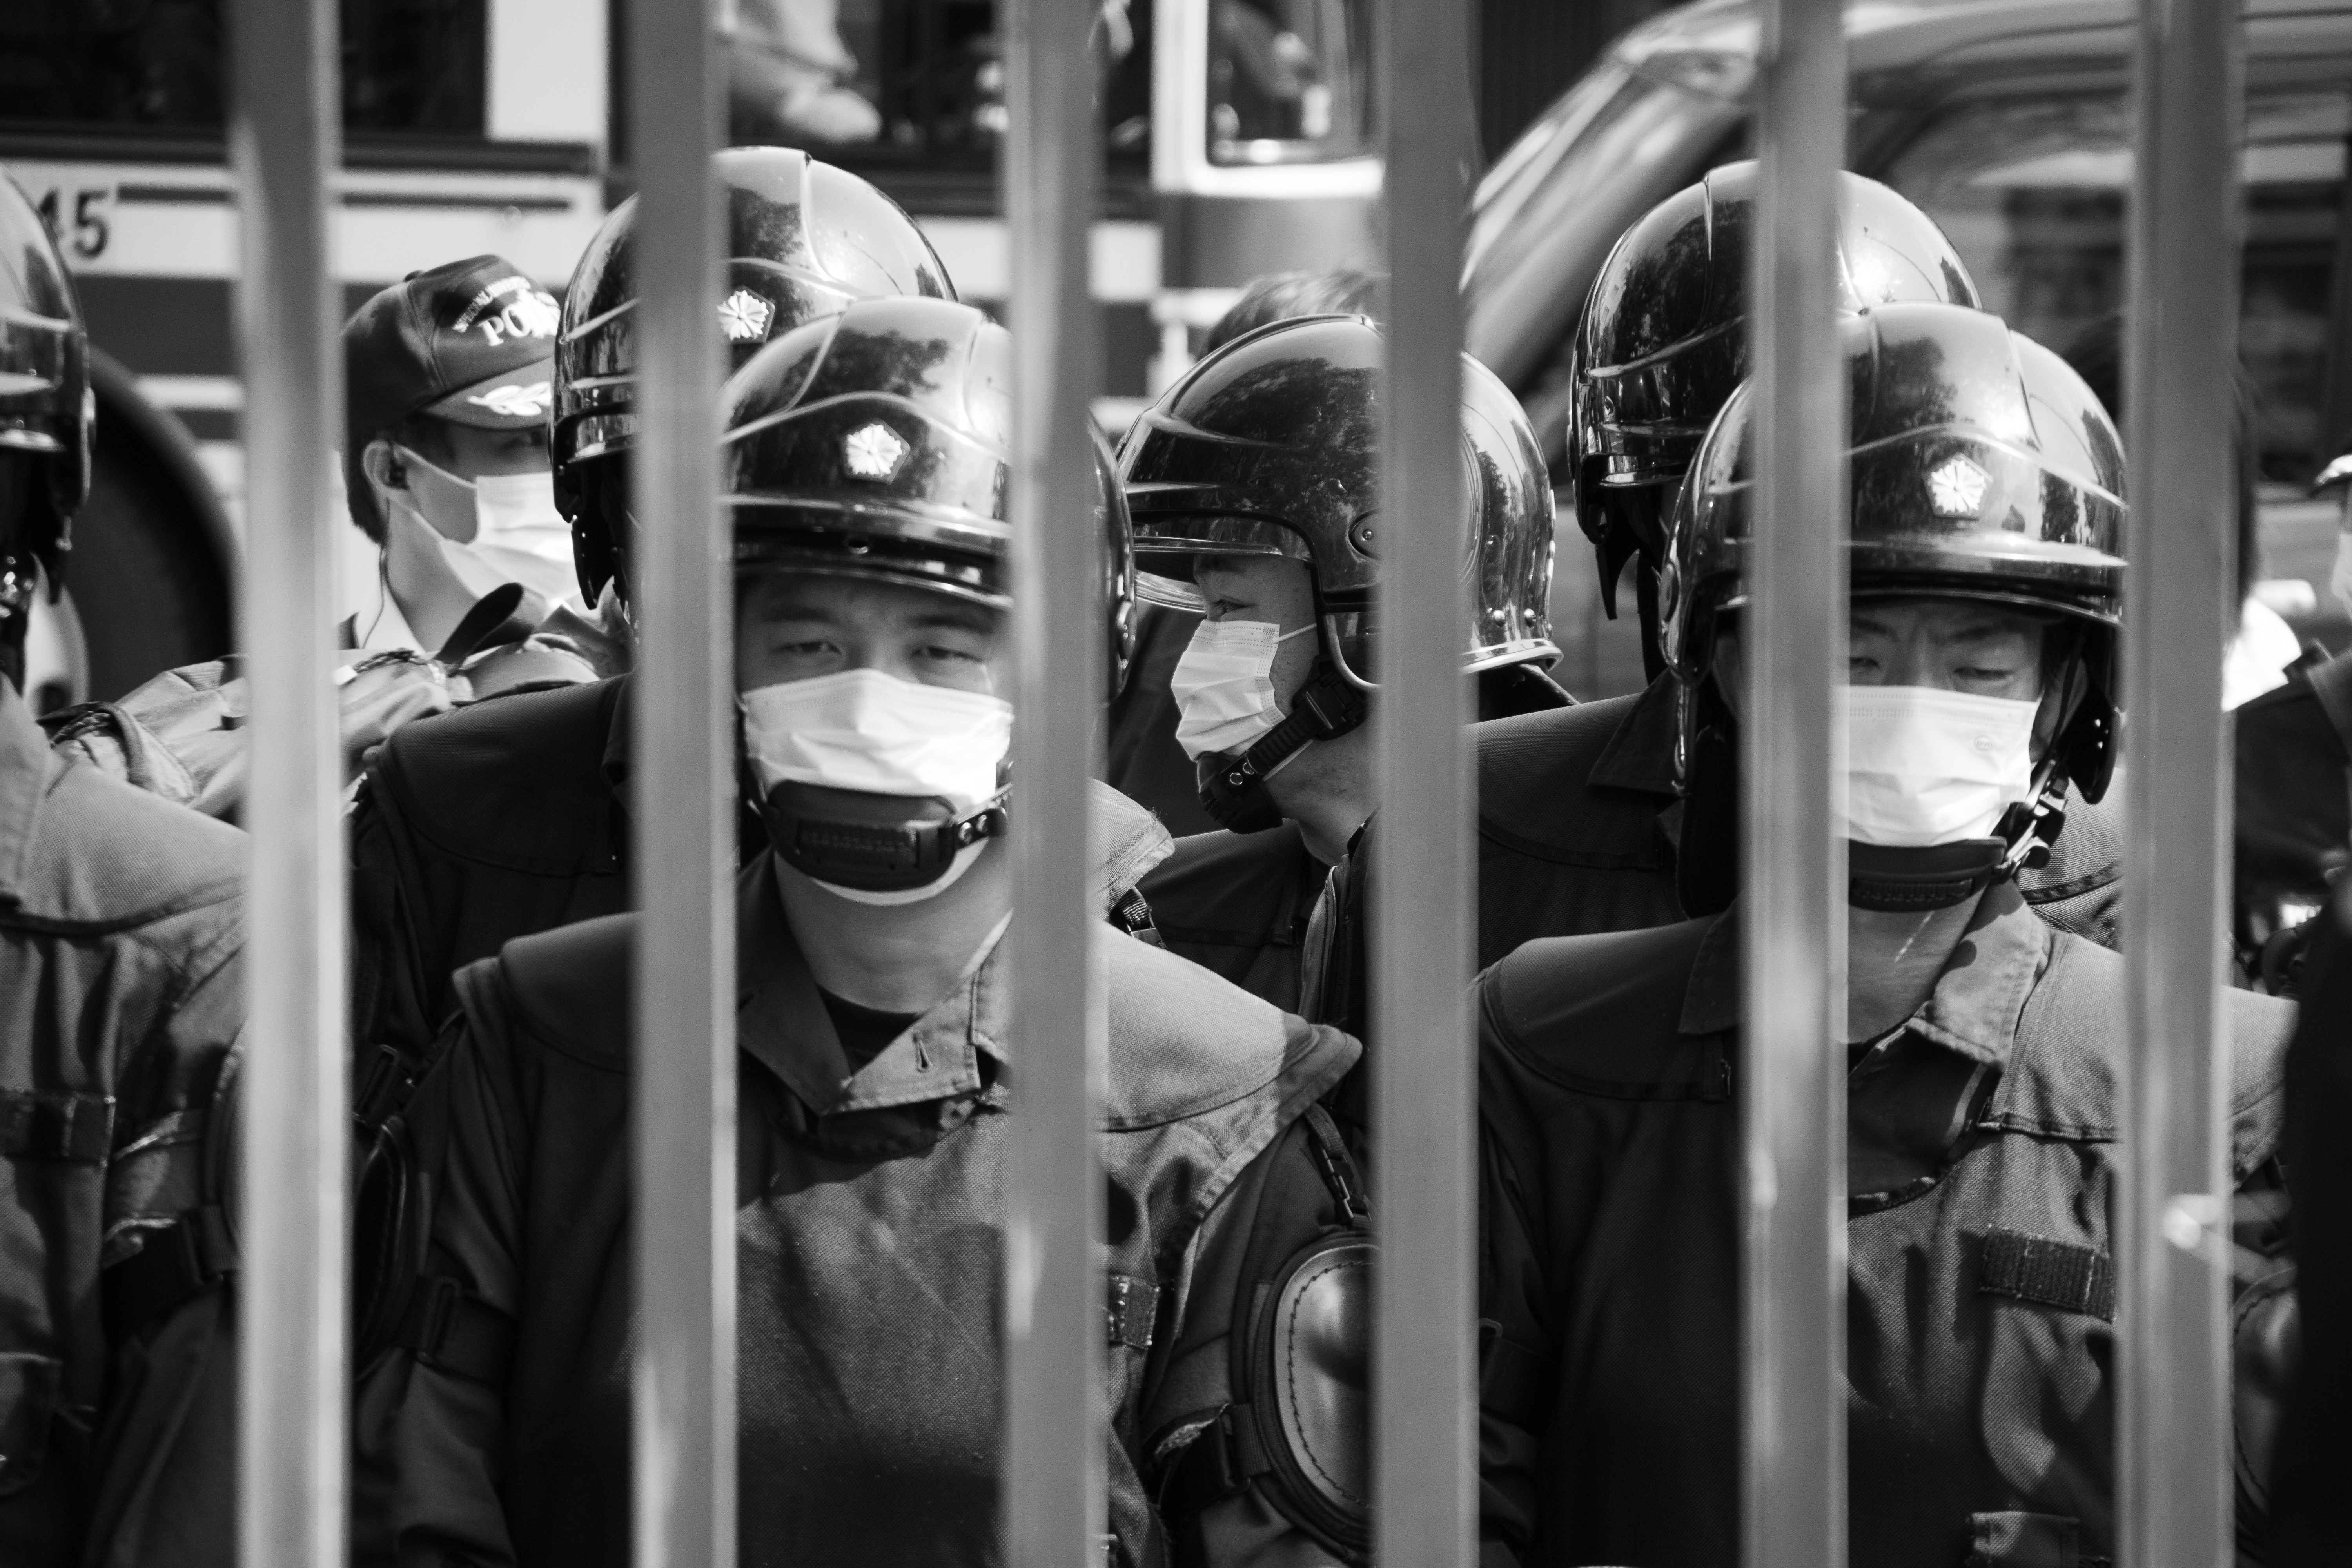
\includegraphics[width=10cm]{gazo/kidotai.jpg}
  \caption*{{\small 封鎖された正門前に並ぶ機動隊}}
\end{figure}



熊野寮生の雨蛙と言います。去る2021年6月24日、僕は初めて自分の家に家宅捜索(いわゆる「ガサ」)が入るという経験をしました(捜索対象は僕の部屋ではなかったですが)。ツイッターではひとしきり盛り上がりましたし、テレビで全国ニュースとして取り上げられたりもしたので、ご存知の方は多いと思います。

この記事はいち熊野寮生の立場から、このガサがどのように見えたのかを書いたものです。ガサのニュースを見て「熊野寮やべーな」と感じた人は多いと思いますが、僕の実感はむしろ逆で「警察やべーな」です。「そんなん熊野寮生の一方的な見方やろ」という声が飛んできそうですが、この記事を読めば、きっとあなたも「警察やべーな」ってなります。

「警察やべーな」ポイントはいくつかあります。

\begin{itemize}
  \item 思想差別的なチョー微罪逮捕がやばい!
  \item 証拠があるとは思えない熊野寮に捜索に来るのがやばい!
  \item メディアを引き連れて、熊野寮を撮影するのがやばい!
  \item 寮生は捜索妨害しないのに機動隊200人連れてくるのがやばい!
  \item 令状もないのに寮生の部屋を覗いたり、バイクのナンバーをメモってるのがやばい!
  \item 実際押収品は寮生のノートたったの一冊!
  \item 熊野寮のネガキャンがしたいだけで草!
\end{itemize}

という感じです。順次説明していきますね。

\noindent *この記事は、あくまでいち熊野寮生としてガサについてどう思っているのかを書いたもので、寮生全員が同じような感想を持っているとは限りませんし、熊野寮自治会の立場でもありません。寮自治会のガサについての立場は熊野寮ホームページから声明「2021年6月24日家宅捜索に関する抗議声明」、あるいは本パンフレットのp.\pageref{sec:gasa_jiti}を参照してください。

\subsection{Aさん逮捕}

今回の捜索は、中核派の活動家であるAさんの逮捕に関連するものです。僕が把握している時系列はこんな感じです。

\begin{itemize}
  \item 6月21日午前 Aさん逮捕
  \item 同日午後 Aさんの京都の\textbf{下宿}などに家宅捜索
  \item 6月23日 Aさんの勾留延長が決定
  \item 6月24日9時ころ Aさんの立ち回り先として\textbf{熊野寮}に家宅捜索
  \item 7月1日 Aさん勾留満期で釈放
\end{itemize}

逮捕容疑は「免状不実記載」、つまり「免許証の更新時に居住実態のある京都の下宿ではなく、実家の住所を書いた」というものでした(誤解が多いかもしれませんが、\textbf{Aさんは寮に住んでいたわけではない}です。寮とは別にAさんの下宿とされるアパートが捜索されています)。今これを読んで、
\begin{quote}
  \fbox{自分も住民票移してへんし、免許証の住所実家や。逮捕されるやん}
\end{quote}
とヒヤッとした人いますよね。そう、免状不実記載なんて親元を離れた大学生とか、単身赴任中の会社員など多くの人がやっていることです(僕は免許証持ってないので大丈夫です)。しかも殆どの人は、それが悪いことであるとそもそも認識していないでしょう。報道では「更新前の住所から変更がないとの虚偽申請をし、免許証に事実と異なる住所を記載させた」などとされていますが、Aさんにも、そして全国の「免状」を「不実」に「記載」している人にも、「虚偽」で「記載させる」意図はないでしょう。実際、警察は「免状」を「不実」に「記載」している人を普通は逮捕していません。いちいち逮捕していたらきりがないですし、そもそも誰かが害を被るようなものでもありません。発覚した段階で注意すればそれで済む話に思えます。

にもかかわらず逮捕される種類の人々がいます。いわゆる「過激派」です。実は免状不実記載という罪状での逮捕は、過激な政治活動家を逮捕するのによく使われる手なのです。警察は過激派(中核派は暴力を用いた社会主義革命を標榜している)を弾圧したいと思っていますが、一方で過激派の一員だからといって常に明確な犯罪を行うわけではありません(というか殆どの構成員は基本的には合法活動しかやっていないでしょう)。そこで免状不実記載というチョー微罪での逮捕が使われるというわけです(当然、起訴には至らず、7月1日に釈放されています)。

熊野寮にいるとよく「活動家への逮捕は殆どは不当逮捕だ」という主張を聞きます。あんまり信じてなかったんですが、6月21日のAさんの逮捕容疑を聞いたとき、初めてその主張に納得しました。\textbf{思想信条の自由は保障されているはずだし、不当な身柄拘束も許されないはずなのに(憲法に書いてある)、国家権力にとって都合の悪い人物はしょーもない理由で逮捕してもいいと、警察や令状を出した裁判所は思っているわけです。}

警察やべーな。こんなので逮捕できるなら誰も声あげられなくなるよ。


\subsection{寮にガサが来る 〜〜探しものはなんですか〜〜}

\subsubsection{ガサの準備をしよう!}

Aさんが逮捕されたときから、熊野寮のガサ準備は始まりました。さっきも言った通り、Aさんは寮に出入りしたことはありますが、住んでいるわけではありません。でもガサが来る可能性は高いという認識が寮内にはありました。熊野寮と関係がなくとも、中核派とされる人物の逮捕には熊野寮ガサが伴うことが多いからです。

ここで寮で受け継がれている伝説的な「\textbf{なんでや熊野寮関係ないやろ}」事案を紹介しましょう。これは2013年4月にあったガサで、東北大生の法政大学(東京)への不法侵入に関連したものでした。この東北大生は\textbf{熊野寮に立ち入ったことは一度もありません}でした。なぜ東京の大学への東北大生の立ち入りの証拠が、熊野寮に存在していると警察や、令状を出した裁判所は思ったのでしょうか。不思議ですね。

今回も、Aさんの下宿とされるアパートには、6月21日(逮捕当日)にガサがあったので、本当にAさんが免状不実記載をしていたなら、ここで証拠が見つかっているはずで、熊野寮にガサ入れする必要性は本来なら(警察や裁判所が憲法に基づいて人権に十分配慮しているなら!)ないですが、それでも準備をしなければなりませんでした。

僕らが準備するときに念頭にあったのは、過去のガサであった「やべーこと」の数々です。

\begin{itemize}
  \item 警察が捜索令状を提示せず寮内に入ったことがある(法令違反です)。
  \item 警察が捜索に大量の機動隊を連れてきて、捜索場所以外の廊下や階段を占拠し、寮生の通行を妨害したことがある(邪魔だし、過剰警備です)。
  \item 警察が捜索場所以外を撮影したことがある(令状がないので証拠の違法収集です)
  \item 警察がマスコミに事前にリークし、寮や寮生を撮影させたことがある(プライバシーの侵害。ガサに対応する寮生が顔をサングラスなどで隠すのはこのため)
\end{itemize}

もちろん令状のある捜索を阻めばこっちも捕まっちゃうので、あくまでやるのは「\textbf{法令通りに捜索が行われるように}」、そして「\textbf{寮生のプライバシーが守られるように}」する準備です。具体的には、寮生の間で令状の確認方法に関する打ち合わせをしたり、正門に「令状を確認すれば案内します」という掲示をしたり(令状提示対策)、B棟窓に「プライベート空間を撮影しないで」という掲示をしたり、著作権の関係で放送できないことを見越してミッキーのお面を作ったり(ミッキーはディズニーの要請で映り込むのさえだめだという噂を元にしたメディア対策)しました。


\subsubsection{ガサが来た!}

% \begin{wrapfigure}[10]{o}[1cm]{6cm}
%   \centering
%   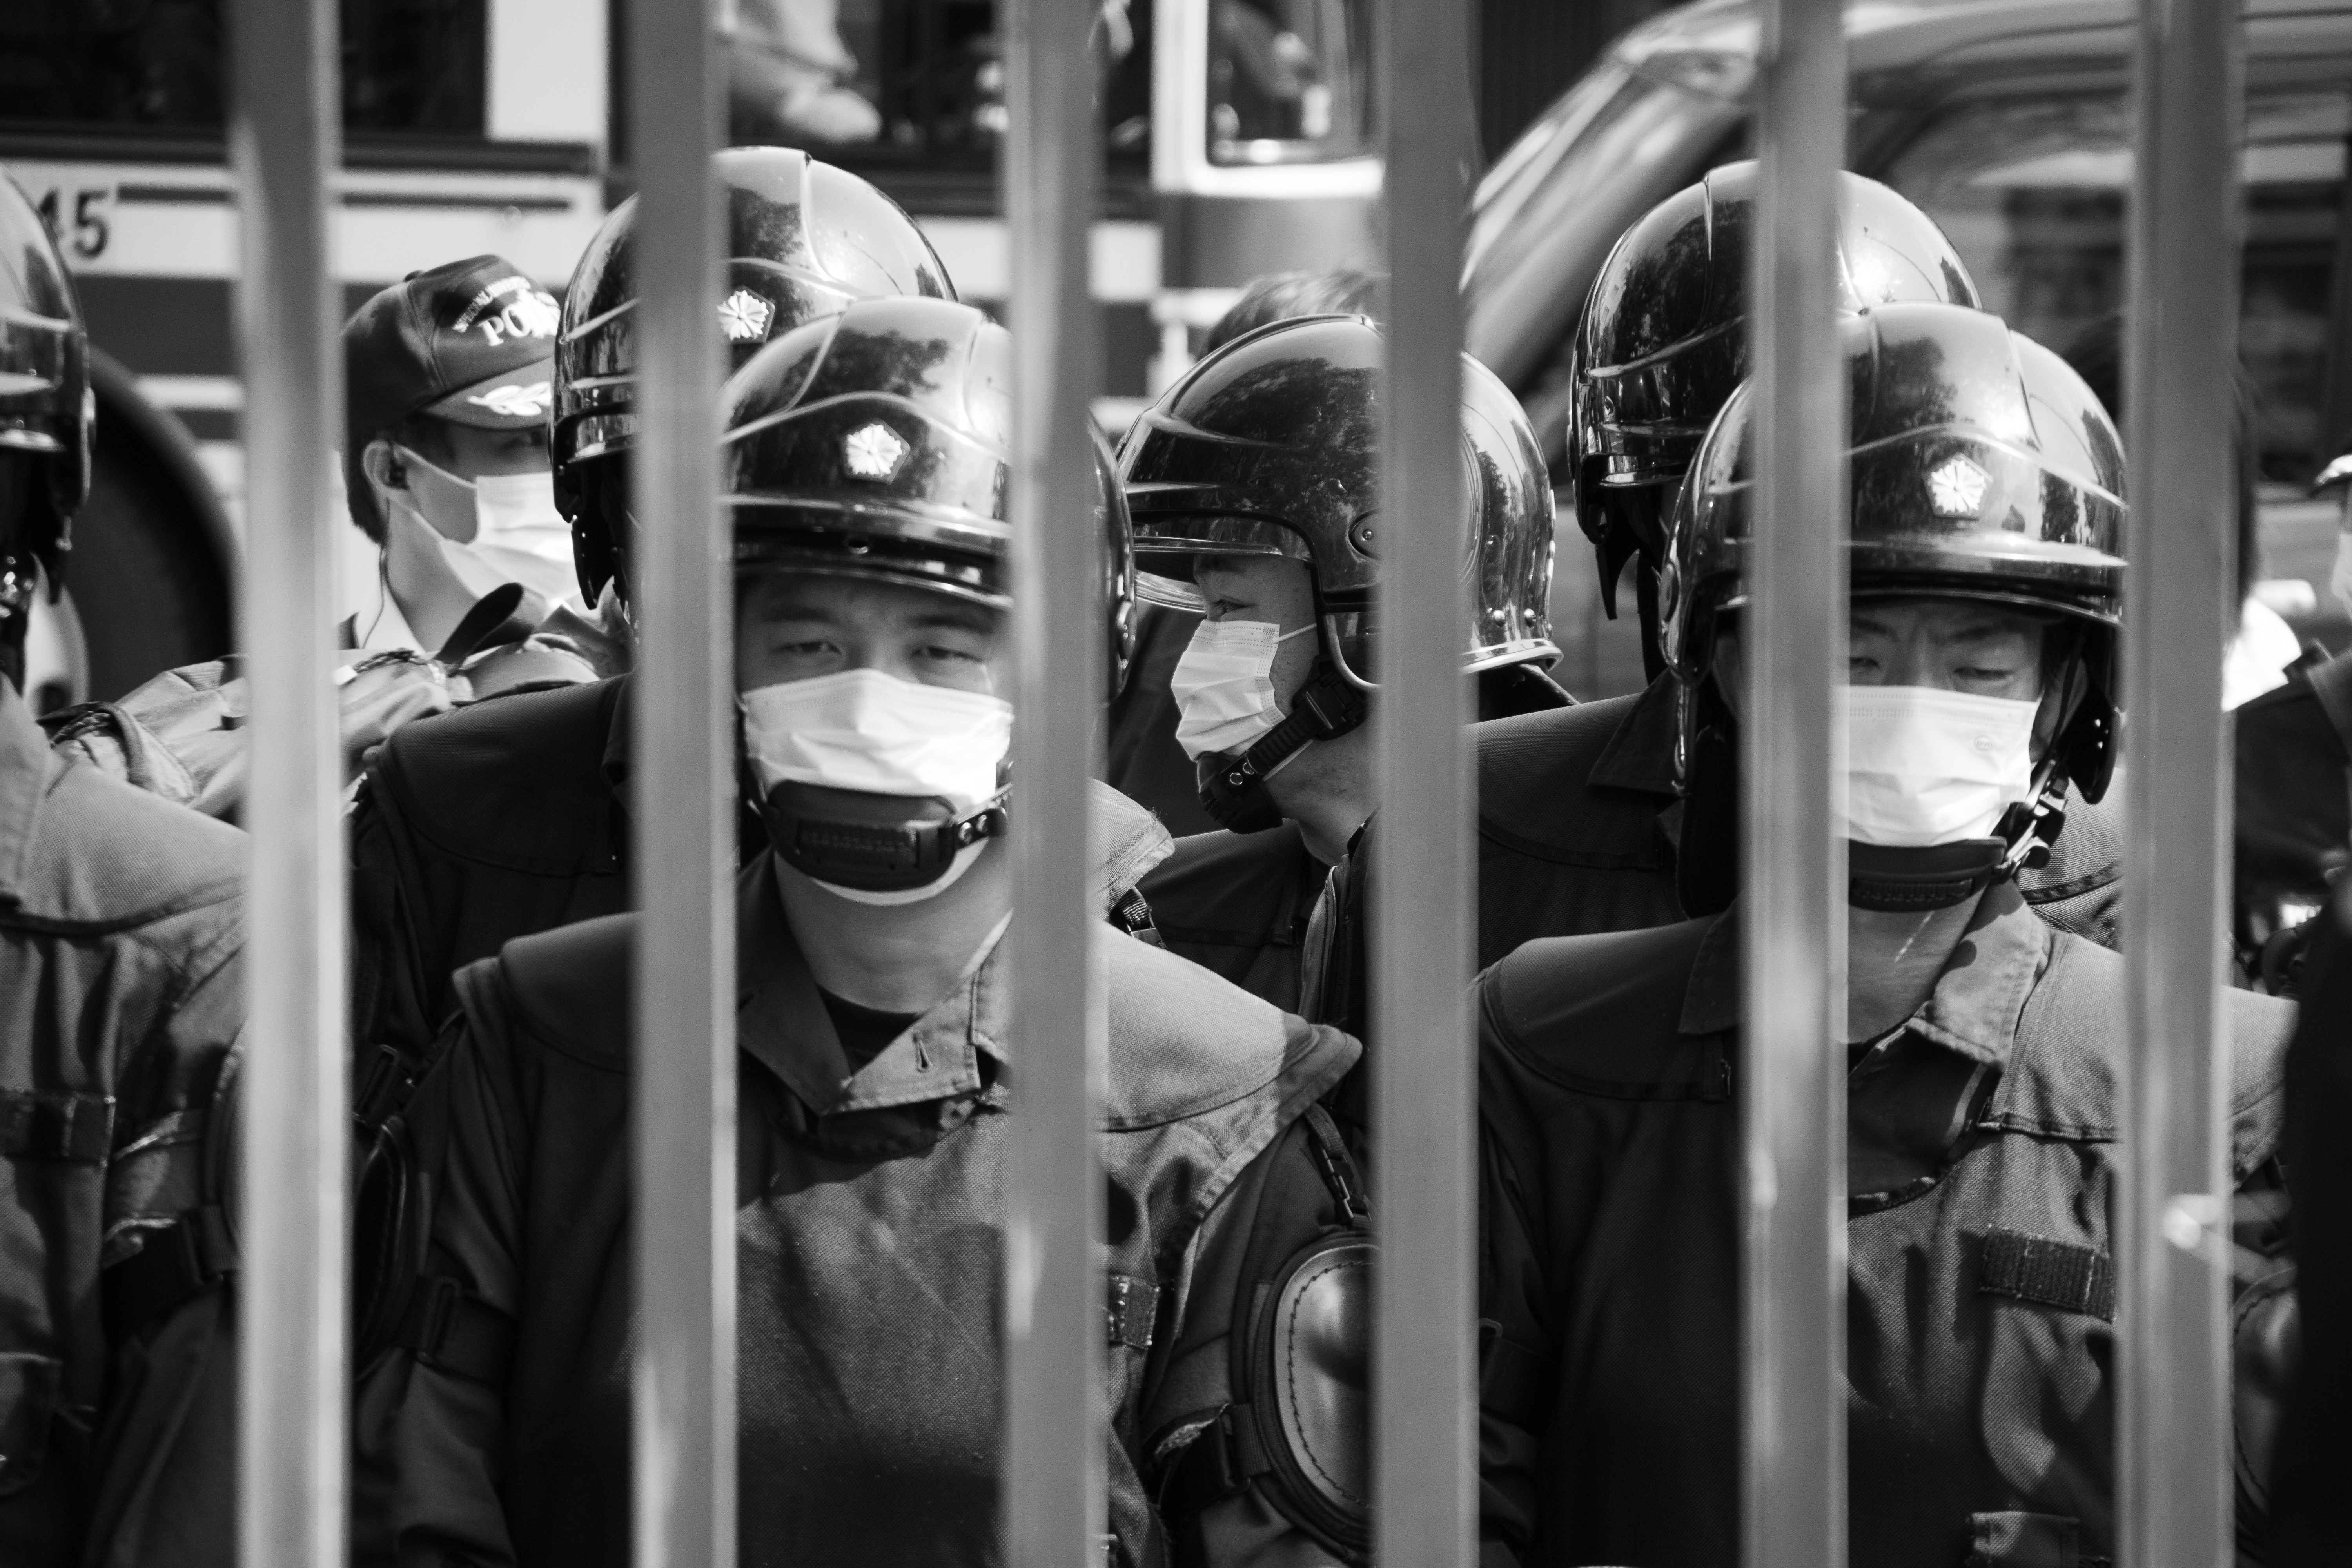
\includegraphics[width=5cm]{gazo/kidotai.jpg}
%   \caption*{{\small 封鎖された正門前に並ぶ機動隊}}
% \end{wrapfigure}

熊野寮は京大の敷地です。学問の自由を定めた憲法との関係から、警察のガサには京大職員の付添が必要です。なので、警察はガサの直前に京大に立ち入る旨の連絡をします(これは熊野寮以外の京大構内に立ち入る場合も同様です)。連絡を受けた大学は熊野寮自治会に対して直ちに捜索の連絡をいれる手筈になっています。

今回の場合は8時45分ころに寮に当局から電話があったので、その時点で熊野寮の正門を封鎖し、正門周辺に寮生がサングラスなどで顔を隠して集合しました。目的は機動隊の寮内雪崩込み占領とどさくさに紛れての令状不提示を防ぐためでした。しばらくすると立ち会いの大学職員と複数台のカメラと記者たちが門前に到着しました。今回もマスコミには警察からリークがあったようです。えろう仲がよろしおすなあ(京都弁)。

\begin{wrapfigure}[10]{o}[1cm]{6cm}
  \centering
  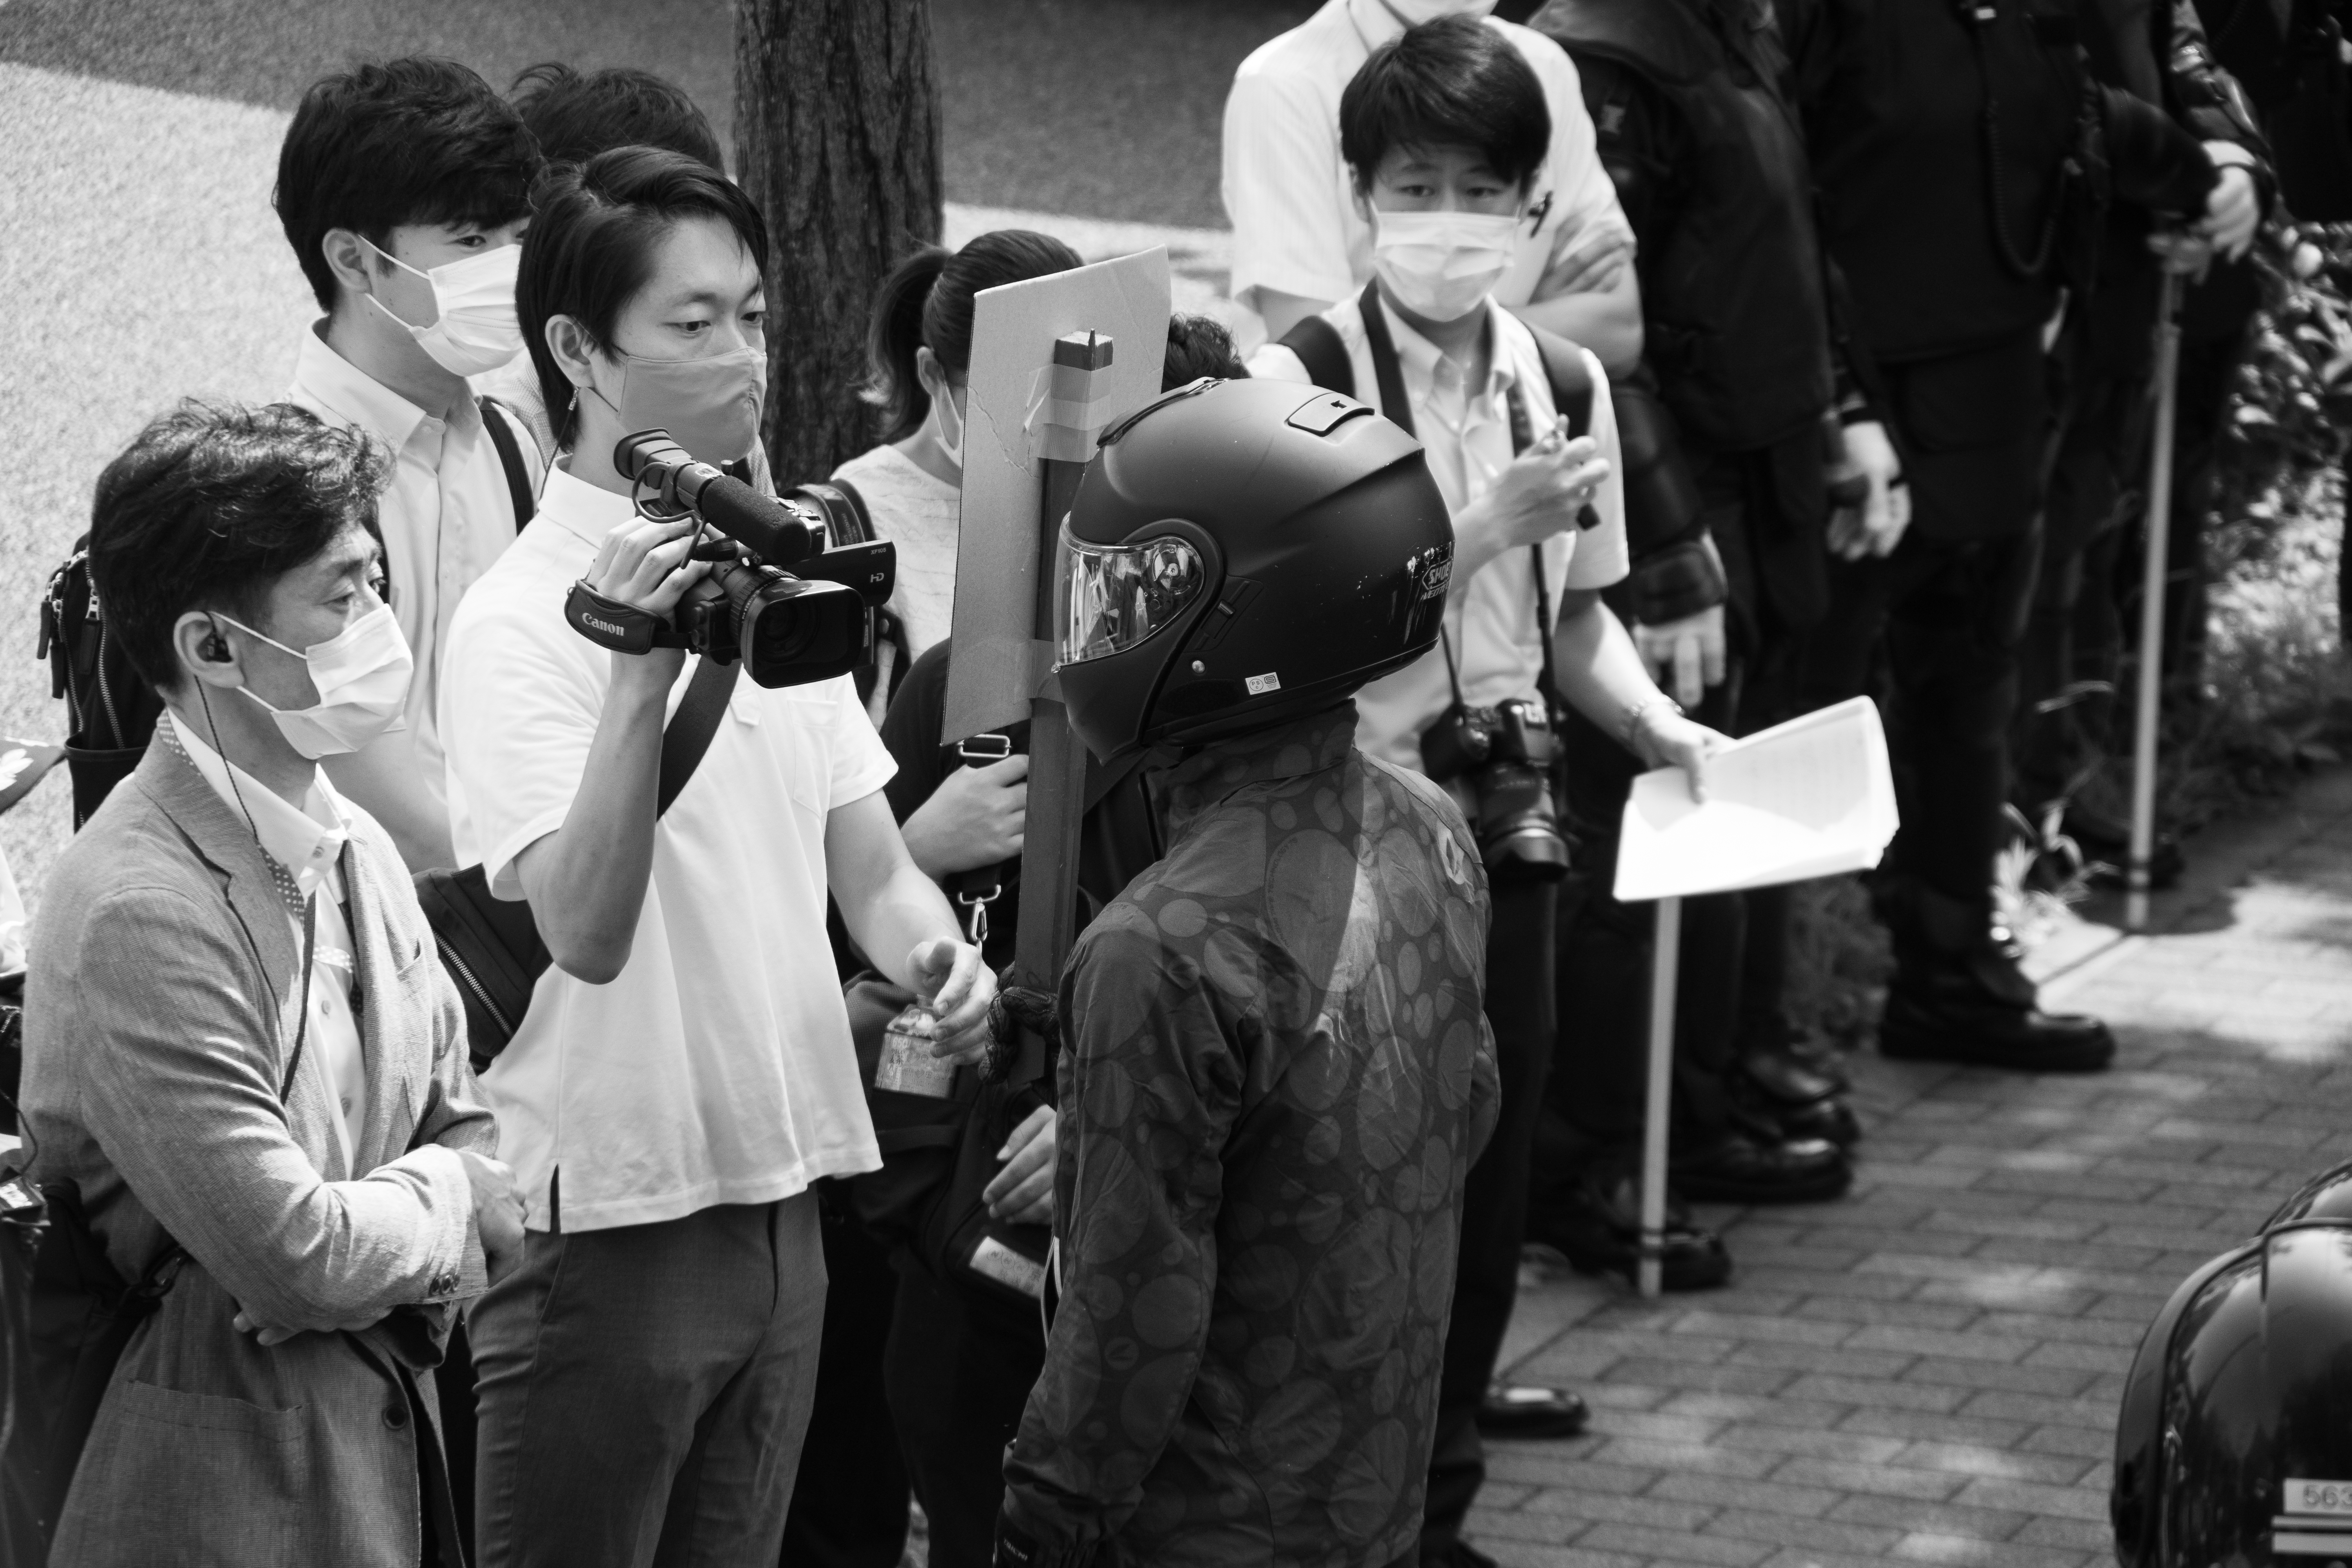
\includegraphics[width=5cm]{gazo/media.jpg}
  \caption*{{\small メディアと対峙。数年前には「顔を隠しているのは全て過激派」などという根拠のない報道があった。覆面をするのはプライバシーを守るため}}
\end{wrapfigure}

捜査員が大量(報道によると200名らしい)の機動隊を引き連れてやってきたのは9時ころでした。「かまぼこ」と呼ばれる護送車が寮の前に停止すると、警棒で武装した機動隊がぞろぞろと降りてきました。先頭には武装はしていないが強面の公安捜査員。門の中で見ていた僕の感想は「あーこれが権力かあ」です。自分が住んでいる場所への明確な敵意とそれを執行するのに十分な武力動員。大人200人あまりが免状不実記載ごとき微罪に動員されたという事実。ちょっと怖かったですが、寮生もそれなりに集まりましたし、何よりこっちには憲法や刑事訴訟法がついているので、心強くもありました。熊野寮門前は途端に機動隊で埋め尽くされましたが、こちらの意図通り無理やり寮内に侵入するということは阻止しました。


\begin{wrapfigure}[10]{o}[1cm]{6cm}
  \centering
  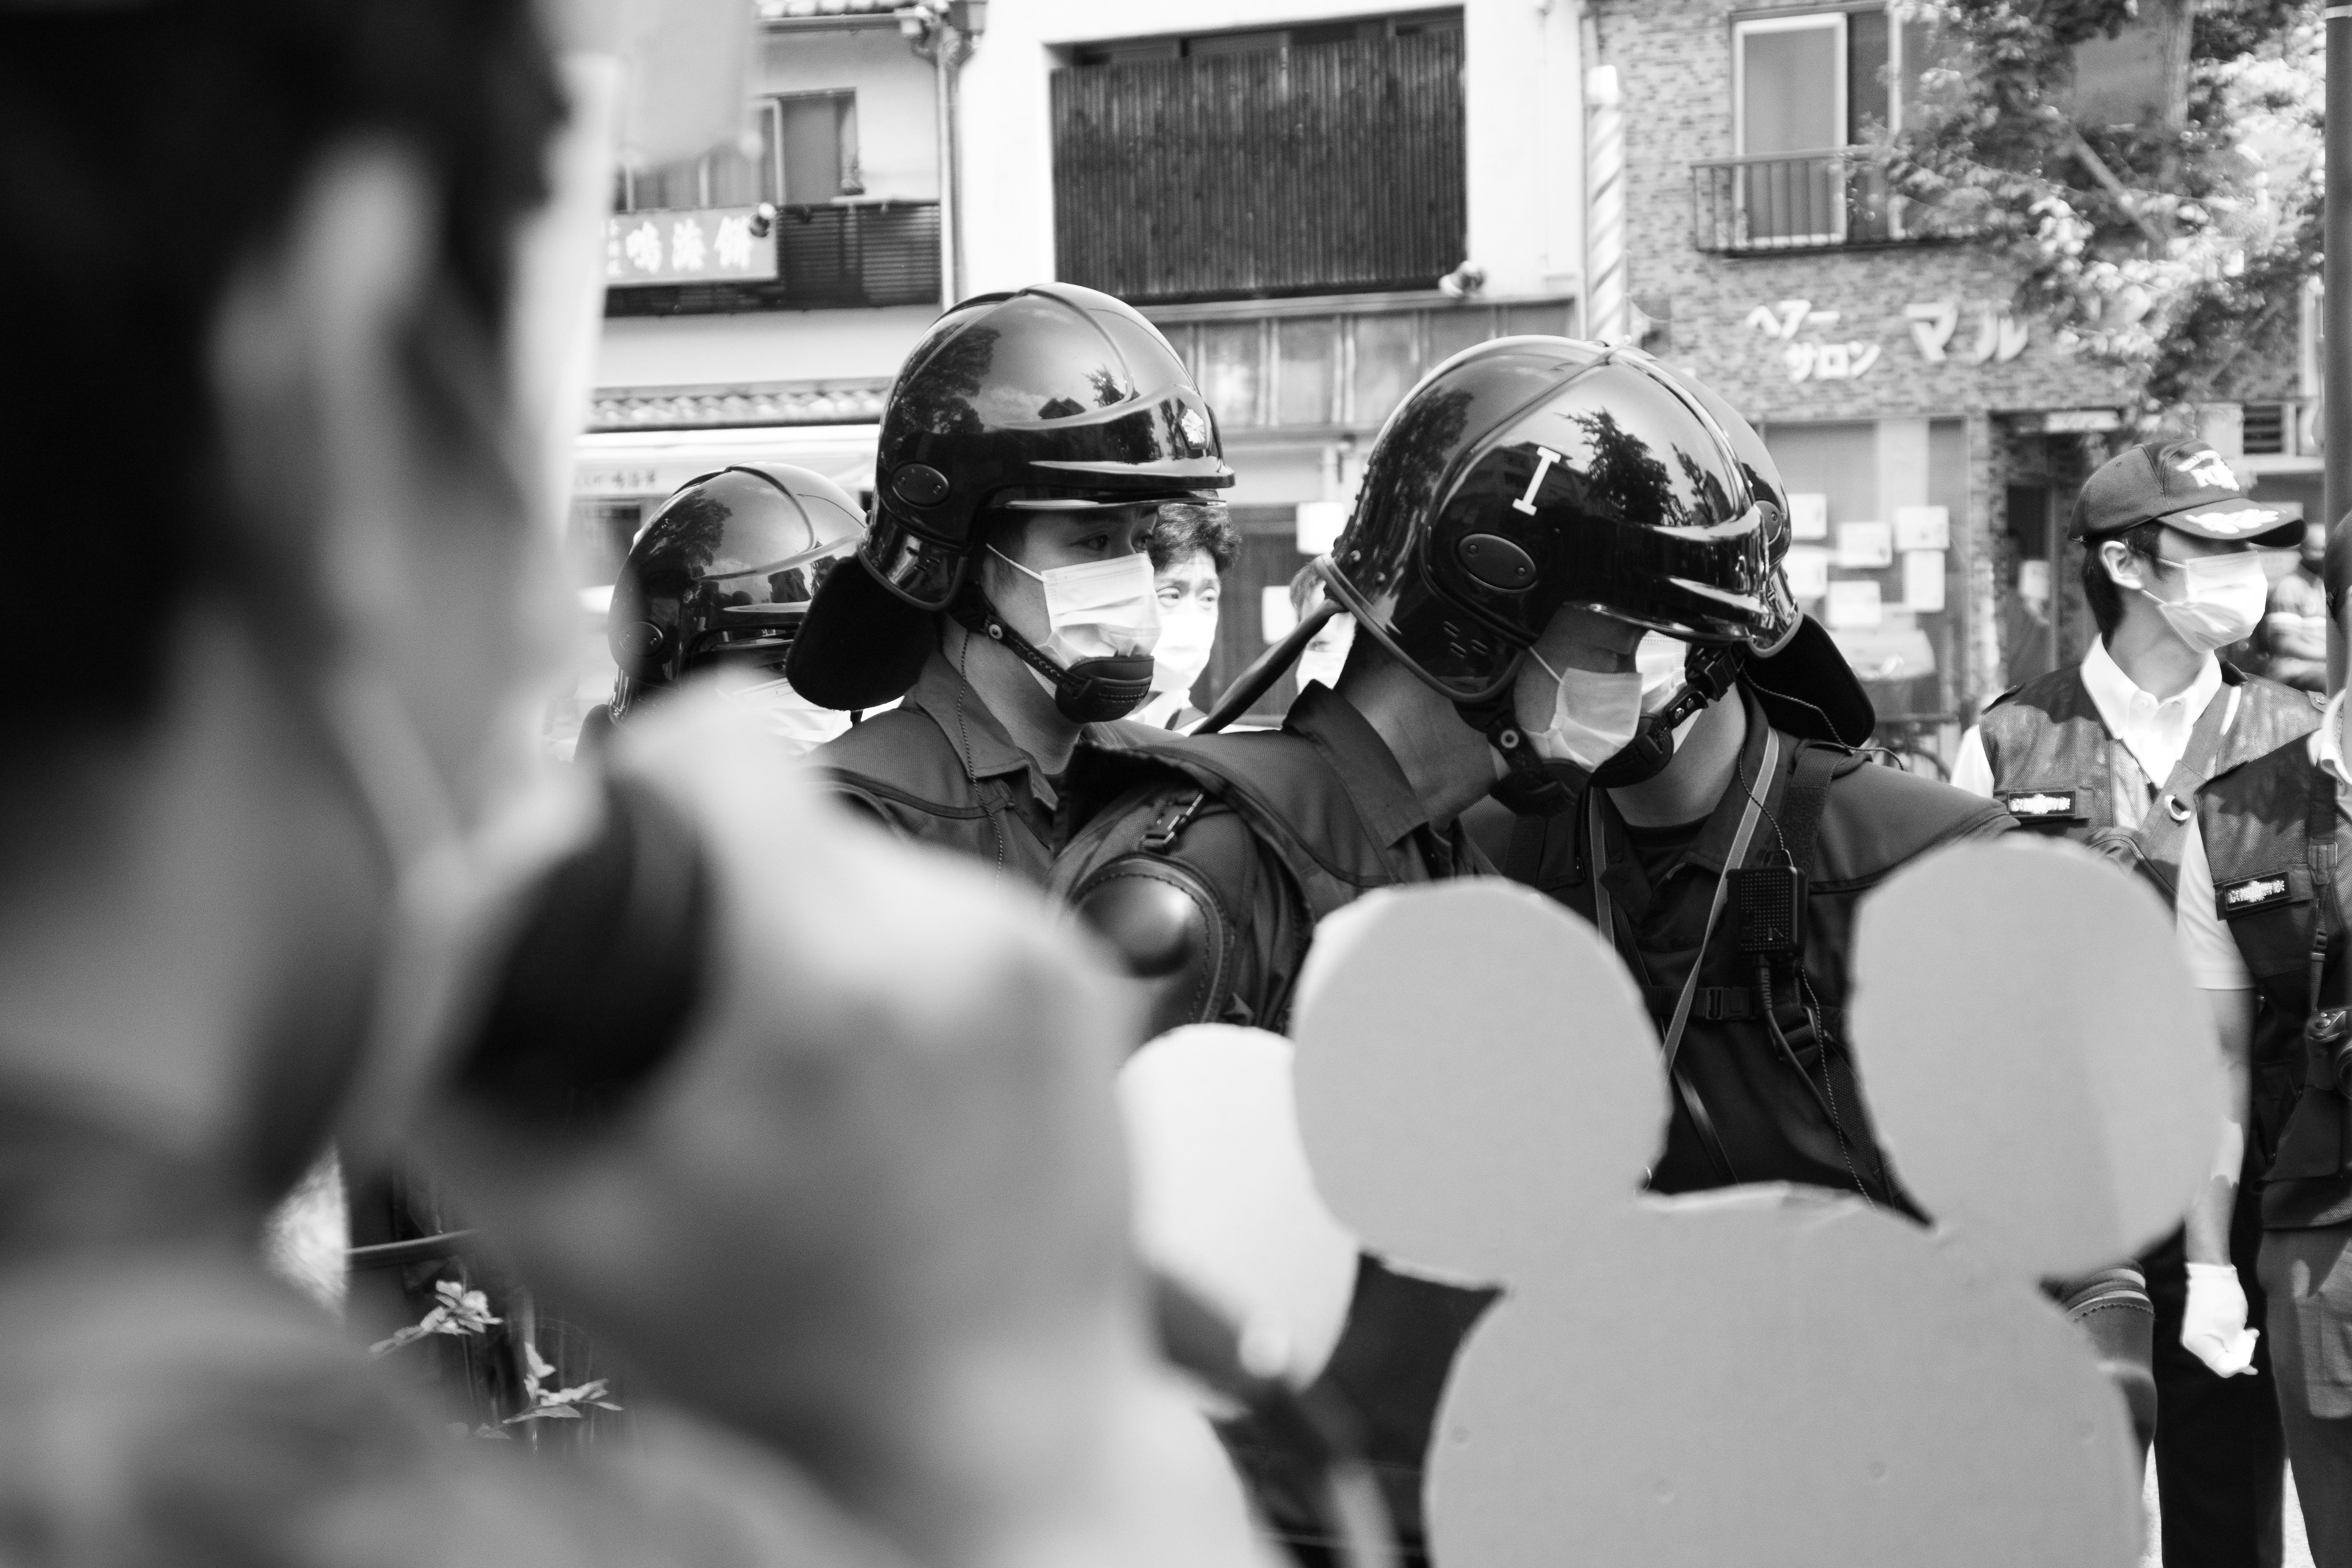
\includegraphics[width=5cm]{gazo/mikki.jpg}
  \caption*{{\small 声が通らないので拡声器を使って交渉。ミッキーのお面も活躍。}}
\end{wrapfigure}

\subsubsection{令状を見せて下さい}




さて、ここから交渉が始まります。まずは令状を見せるように言いました。それに対して捜査員は「捜索立会人(部屋等の捜索にあたっては、その部屋の住民などの立ち会いが必要)に見せる」という趣旨の主張をしてきました。しかし、寮内に立ち入るにも関わらず、寮生に令状を見せないということが許されるのでしょうか(本当に令状を持っているかわからない警察を寮内に入れることは当然できません)。そこでこちらは「法令に則って、ここで呈示して下さい」と反論すると、捜査員は「ここで議論はしない」と叫び、「捜査妨害するんですか」と威圧してきました。こっちも絶対に公務執行妨害で逮捕されたくないので「令状を確認すれば捜査には協力する。法令に則って令状を呈示してください」とメディアにも聞こえるように必死に叫びました。

\begin{wrapfigure}[10]{o}[1cm]{6cm}
  \centering
  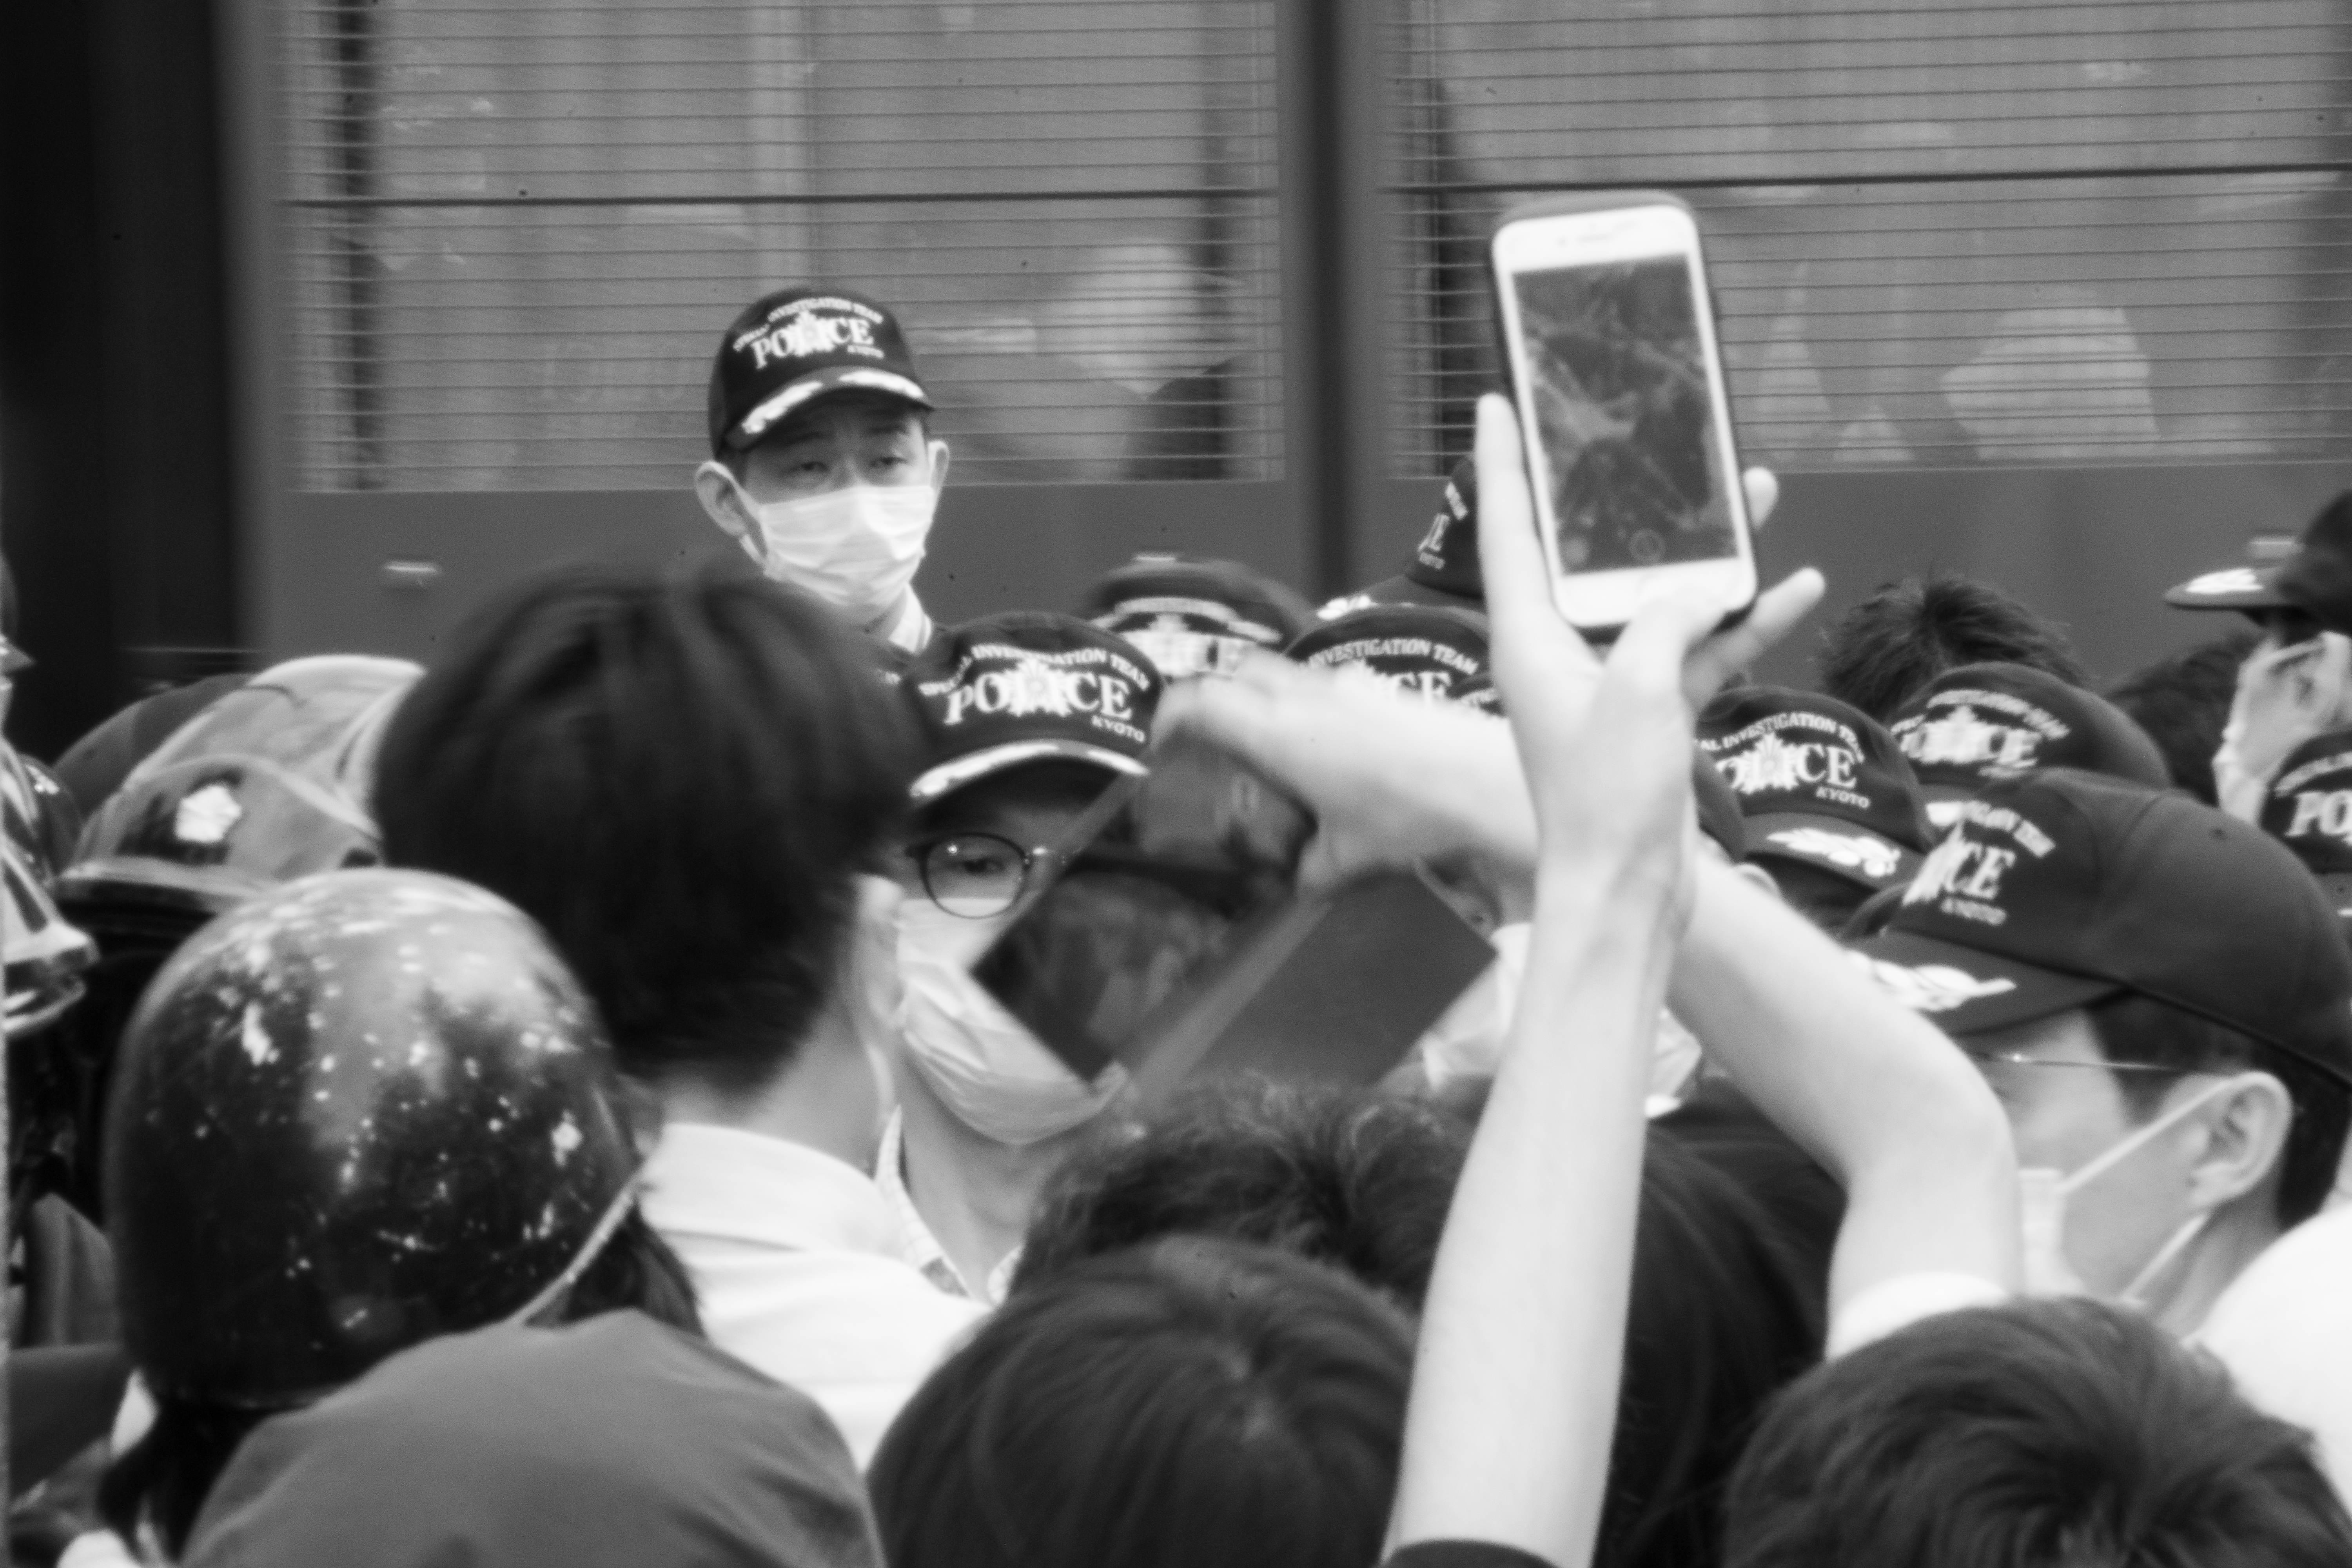
\includegraphics[width=5cm]{gazo/rejo_yomiage.jpg}
  \caption*{{\small 令状読み上げのシーン。警察は令状を撮影されることを拒んだ(背景の車が「かまぼこ」)}}
\end{wrapfigure}


2,3分押し問答した結果、令状は呈示され京大職員と寮生で読み上げました(ただし、捜査員がしっかりと見せてくれなかったので読み上げは不十分でした)。法的根拠なく令状の呈示を渋っていたとすれば、「警察やば」案件ですね。




\subsubsection{機動隊は入らないで下さい}

「令状見せてもろたし、ほな案内しまひょ」とはならないですね。捜査に機動隊は必要ないですから。捜査をするのはあくまで武装してない捜査員です。機動隊は過去に法的根拠なく寮内の廊下や階段を占拠したことがあるのは前述の通りです。つまり邪魔。こちらとしては、機動隊を寮内に入れる訳にはいきません。「捜査に協力するので機動隊を引かせて下さい」と主張すると「それはこっちで判断する」。「ここでは交渉しない。君らがこんな人数で妨害するから必要なんや」と叫ばれました。やっぱり逮捕されたくないので「あなた達が過剰警備をしているので抗議しているだけで妨害の意図はありません」と負けじと叫びます。

同様の押し問答のあと、寮生の主張が受け入れられました。\textbf{結局、機動隊は捜索の警備に必要なかったようですね}。機動隊員1人につき1万円の日当が支払われていたとすれば、少なくとも200万かかっている計算になります(ガバ計算)。僕たち寮生を脅したかったのか、それとも予算を消化したかったのか、どっちなんでしょうねえ。えらい仰山で来はって、賑やかどすなあ(京都弁)。


\subsubsection{令状のないプライバシー侵害}

捜索中にもやばい点がいくつかありました。僕が直接見たわけではなく、他の寮生から聞いたものですが、\textbf{捜索場所以外の部屋}の中を扉が開くたびに捜査員が覗き込んだり、駐輪場のバイクのナンバーをメモするなどしていたらしいです。令状はないので、ただのプライバシーの侵害です(当然、憲法・法令違反)。やばいですね。


\subsubsection{押収品について}

さて、寮内に入らなかったとは言え、200人もの機動隊を動員して行われたこの大規模な捜査で何か見つかったのでしょうか。捜索を受けたのは2箇所です。ここに2通の文書があります。
\begin{figure}[h]
  \begin{minipage}{0.5\textwidth}
    \centering
    \includegraphics[width=8cm]{gazo/oushuhinmokuroku.jpg}
    \caption*{{\small 押収品目録}}
  \end{minipage}
  \begin{minipage}{0.5\textwidth}
    \centering
    \includegraphics[width=8cm]{gazo/sosakushomesho.jpg}
    \caption*{{\small 捜索証明書}}
  \end{minipage}
\end{figure}

それぞれの部屋でどんな証拠が押収されたのかを示す警察が発行した文書です。1つ目は押収物目録。押収されたのはノート一冊とあります。もう一つは捜索証明書。これは、押収物がなかったときに捜索がすでになされたということを証明するための文書で、日本でこれが発行されるのはかなりレアです。なぜなら証拠が確実に見つかる場合にしか捜索はされないからです。ネット上では刑事訴訟マニアによって高額での取引がされているとか、いないとか。

\textbf{つまり今回の捜索では、寮生の私物のノート一冊しか押収していないのです。}しかもこのノートの持ち主によると、Aさんの免状不実記載についての記述はこのノートにはないそうです。\textbf{さすがに手ぶらで帰るというのは警察のメンツ的にまずかったのでしょうか。}つくづくやばい組織ですね。

なお「400点もの押収品があった」というテレビ報道もありましたが、大嘘もいいところですね。警察とそんなに懇ろなんだったら嘘掴まされるなよ。お前らいいように使われてるだけやぞ。真実を報道しろ。ボケナス。

すいません。怒りが漏れてしまいました。


\subsection{ガサと寮生}

\begin{wrapfigure}[15]{o}[1cm]{4cm}
  \centering
  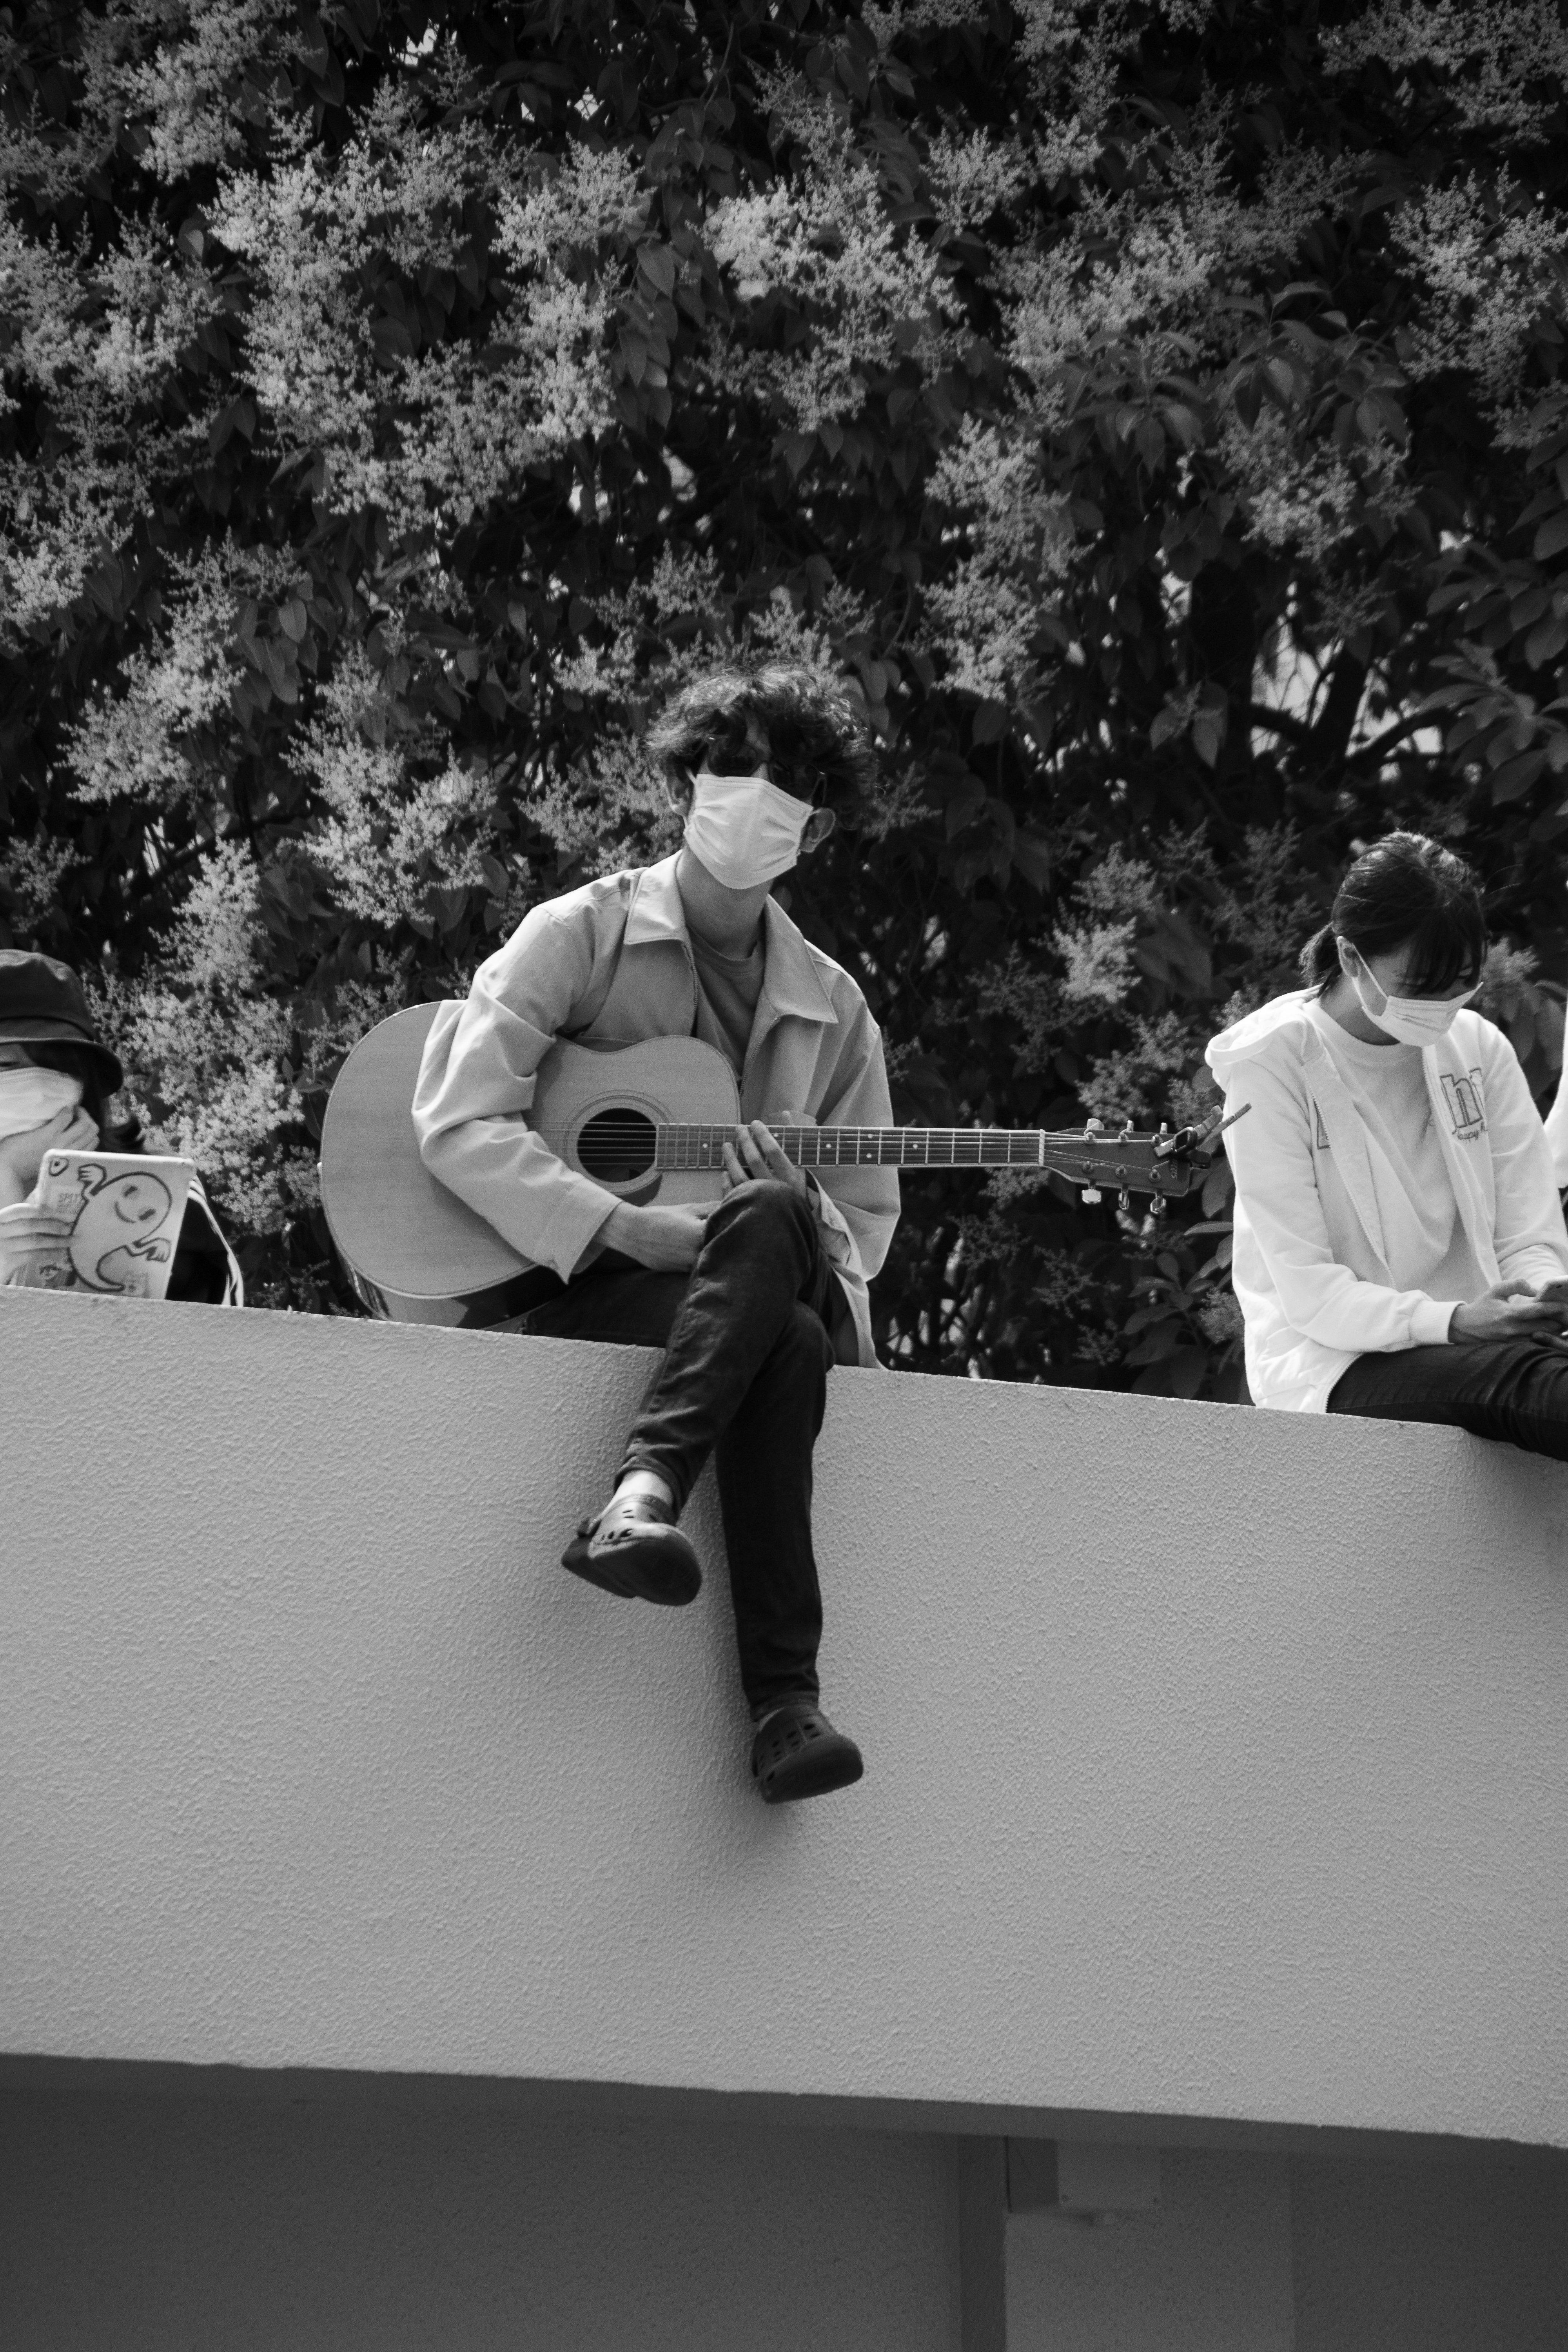
\includegraphics[width=3cm]{gazo/live.jpg}
  \caption*{緊急ライブ(演目はスピッツ「チェリー」など)}
\end{wrapfigure}

ガサが来た日は京大の授業日でした。機動隊の隣をすり抜けて大学に向かったり、授業には行かずに警察の対応や抗議をしたり、警察と世間話をしたり、メディアの撮影に抗議したり、報道カメラマンみたいに動き回って写真を撮影したり、屋上で眺めたり、ラブ\&ピースを訴えて緊急ライブをギター1本で開催したり、ガサには興味なく部屋にいたり、寮生はいろいろな仕方でガサの時間を過ごしました。僕は寮を守りたいという気持ちで正門前でずっと警察の対応をしていました。捜索の不当性や過去にあった違法な捜索の事例は寮内でだいたい共有されていると思いますが、ガサにどう向き合うかは個人に任されています。中には「ガサって楽しい」と思った寮生も多いと思います。不当な権力と、みんな一緒に法律(とミッキーのお面)片手に対峙することである種の興奮が生まれるのは当然です。僕もちょっぴり楽しかった。




けれど、忘れてはいけないのは、\textbf{今回の逮捕やガサは明白な人権侵害だということ}(上でも述べたとおりです)と、単純にガサが迷惑な人も多いということです。授業に普通に行きたかった人もいましたし、熊野寮のガサで友人や親から心配されたり、「熊野寮に住んでいるなんて危ない人だ」と偏見を持たれたりした人も多くいます。僕もやりましたが親への説明が結構面倒なんですね。この記事が親の説得に役立てばいいなあ。


\subsection{まとめ}

いかがでしたか。結局、警察が熊野寮に捜索に来た理由はわかりませんでした。

というのは嘘でおおかたの理由はわかります。\textbf{要は熊野寮のネガキャンです。}熊野寮は機動隊付きでガサが来るような場所ですよ、「やばい」場所ですよと、メディアまで動員して宣伝をしているわけです。寮外から見たら、実際そのように見えていたでしょう。でも寮の中から見たら、警察の方が遥かに「やばい」のです。その風景をみなさんと少しでも共有できればありがたいです。

\rightline{写真提供:みかみかみ(ツイッター\url{@mikamiormi})}

{\scriptsize この記事は、webサイト「千万遍石垣」に2021年10月12日に投稿した記事を修正したものです。}


  \clearpage
  \subsecnomaru
%\subsectionを◯なしに

\section{すきあらばけいおん}
\label{sec:suki_kon}

\bunsekisha{文責}{京大全学けいおん斗争委員会(京大全K斗)\quad twitter\url{@sukiarabakeion}}

\subsection{0.ごあいさつ}

\emphbf{
寮祭企画「すきあらばけいおん」\\
熊野寮祭。食堂モニターが空いているすきを見つけて「けいおん!」を見よう。唯の生誕祭をしよう!豊郷行こう!左京区を歩こう!
}

入試お疲れ様です!去年の熊野寮祭では、こんな企画があったとさ。この文章ではけいおんの名シーンを解説するよ!Twitterでもけいおんの名シーン解説をやっています。京大生と桜高生の生活圏はほぼ一致してるので、けいおんを見ると毎日の通学が聖地巡礼になって楽しみになりますよ。

\subsection{1.団結の力}

\begin{quote}
  \emphbf{
    革命的りっちゃん「どんな理由があろうとな!歌ったらアカン歌なんかある訳ないねん!うちらの団結があれば相手が国家権力でもおんなじや!うちら、友達もせんせいもみんな皆に団結拡大して、機動隊なんかデコピンで倒せんねん!」

    反革命むぎちゃん「まあまあ、落ち着いて…お菓子はいかがですか?」

    (OVA「けいおん!免許合宿・京北鹿ロードキル編」より)
  }
\end{quote}

ライブでイムジン河を歌おうとしたHTTを弾圧する桜高当局。りっちゃんが弾圧に対してキレたのを止めようとするむぎちゃんはここではナンセンスであると思います。りっちゃんの決起は正当な怒りに根拠づけられたものです。お菓子で懐柔するのは反革命ですね。でも、こんな状況では誰でも咄嗟にむぎちゃんみたいな行動を取っちゃいそうですよね。これをちゃんと総括してHTTはもっと大きな団結を生み出すバンドになるんです。むぎちゃんは階級的視点を手に入れて、実践します。悪いブルジョワになんか絶対にならないんです。それくらい団結の力は強いよ!

\subsection{2.オルグ}

\begin{quote}
  \emphbf{
    唯へ

    久しぶり。元気にしてる?

    12月9日に京大で、大学当局による学生への懲戒処分に反対する集会をします。唯も職場の組織化で忙しいと思うけど来ない?全国から仲間が集まって発言してくれるから、きっと唯にとっても学ぶことが沢山あるはず。ぜひ来てください。

    真鍋和

    \tatespace
    曽我部先輩 

    ご無沙汰しております。先輩はいかがお過ごしですか?私が熊野寮に入り、活動家になって早いもので13年が経ちました。入寮した翌年の学生ゼネストに突撃してくる機動隊を見て私は衝撃を受けました。「普通に」生活していたときには見えざるものだった権力が、階級闘争の前線に立った瞬間に剥出しの暴力でもって迫ってくる、破壊的な経験。私はそれ以前も社会に関心を持っていたつもりでしたが、権力が「見えざるもの」である限り、私も秩序の中で踊らされていたことに気づいたのです。でも、そこから闘いに決起するまでに長く苦しい時期がありました。…

    (中略)

    またお会いしましょう。 

    真鍋和

    (OVA「けいおん!全学自治会再建編1」より)
  }
\end{quote}

12月26日はゆいちゃんの幼馴染であるのどかちゃんの誕生日でした。桜ヶ丘高等学校卒業後、K大法学部自治会の委員長を務め、熊野寮に入寮して、バリケードストライキで放学処分を受けてなお斗いつづける我らが真鍋和同志の書いた手紙です。


\subsection{3.非和解性}
\begin{quote}
  \emphbf{
    平沢唯「12月集会で職員に『金持ち学生ばっかなんやろ、羨ましいわ』と面と向かって煽られて、久々に切れた。こっちは学費払えんくてどんだけ不安やった思とんねん。まじで次見たら張倒してまいそうやわ。中間管理職か何や知らんけど、へらへら話してきよる時もこっちは処分されるかもしらんねんぞ。」
    (OVA「けいおん!全学自治会再建編2」より)
  }
\end{quote}

唯ちゃんが集会で職員の挑発を受けるシーンですね。職員と馴れ合うことはあまり得にならないのでやめた方が良いということを唯ちゃんはこの時はっきりを悟ったようです。「非和解」という言葉は、階級間の対立の投射にのみ使いましょう。日常で不快なものに、いちいち非和解と言っていたらあっという間に分断されちゃいます。それこそ権力の思う壺ですね。


\subsection{4.確信}
\begin{quote}
  \emphbf{
    平沢唯「以前は私はニヒリストだと思っていた。でも、内省すると、ばらばらの階層の信念が私にも存在することを観察した。しかし、いざ、それに基づいて実践しようとするとき、私はそれらの信念を一体系に配置するところのものを知らぬことに気付き、おののく。どうすればよいか?」

    琴吹紬「体系というものは生きていくのに必要なものだ。しかし、それ以上に役割があるのか疑うことができる。全体を生きられない人間にとって似つかわしいものが体系。選択の問題だ。」

    秋山澪「それでは相対主義に出戻りするだけではないか!私の信念が信念たるには、他者との共有可能性、もしくは少なくとも行動において大きな障害を産まない程度の伝達可能性、もしくはそれを少なくとも日常のレヴェルで前提していて困らない程度のそれがないといけないんだ…。」

    (映画「けいおん!根源悪編」より)
  }
\end{quote}

自分の思想を検証しようとして相対主義に陥った唯ちゃんが回復してくる治療の過程を描く新作映画のワンシーンですね。こういうのって2回生くらいで悩む人が多いイメージがありますね。

\subsection{5.革命的展望}

けいおんのみんなが京大にも息づいていることを感じたことでしょう。今年の寮祭でももちろん「すきあらばけいおん」はおこないます。みんなでけいおん見ようね。

\subsecdefault
%\subsectionのデザインを元に
  \clearpage
  \section{C12新入寮生座談会} \label{sec:C12}



\subsection{自己紹介}

\jinbutu{ニックネーム:午後三時}
農学部森林科学科1回生。予備校の都会感が苦手で森林に。寮のパンフが好きで、2022年の受験時は熊野寮、吉田寮、地塩寮、各寮3冊ずつ(閲覧用、保管用、布教用)計9冊もらって帰った。一応この座談会の企画者。

\jinbutu{ニックネーム:豆板醬}
文学部1回生。C12の1回生の中で唯一の現役生にして十代とは思えない落ち着きを放っているらしい。よく(ずっと)談話室にいてダラダラしてる。大学にはいない。C12随一の麻雀狂い。勝つと上機嫌、負けると不機嫌。(良くない)

\jinbutu{ニックネーム:つむぐ}
経済学部1回生。音楽科の高校でフルートを中心に学び、卒業後は一年間無職として自宅に引きこもり、昨年の春に晴れて社会的身分を得ました。最近は曲作りが楽しい。

\jinbutu{ニックネーム:かぼちゃ}
D2、最近は寒すぎて談話室のこたつに生息、そろそろ常夏のマレーシアに調査へ

\jinbutu{ニックネーム:nob}
理学研究科M1。まーじゃんたのしい

\jinbutu{ニックネーム:半分}
自己紹介:文学部一回生。現役のとき通ってた高校に受けたくもない大学を強制受験させられて浪人したらしい。寮にいない、いつもあちこちフラフラしてる。

\jinbutu{ニックネーム:がみん}
自己紹介:1浪3留理学部7回生。訳あってこの春入寮した。このパンフレットが配られている頃には卒業が確定しているはず(お願いだからしてくれ)。C12に麻雀文化を持ち込んだ人。好きな役は大七星。談話室でアメフト見るのが一番の娯楽。



\begin{multicols}{2}
  


  \subsection{スタート!}

  \talker{豆板醤}おぉー!

  \talker{午後三時}いぇーい!

  ぱちぱちぱちぱち

  \talker{豆板醤}:ギスガンガンガンガンガンガンガンガンガーン!!!ウォウオ!ウォウオ!!(M1グランプリの曲)

  \talker{nob}いやー最近寒くなってきましたねぇ~

  \talker{半分}いやそうじゃないでしょ座談会って

  \talker{豆板醤}言うてやらせてもらってますけれどもー

  \talker{nob}M1のノリだね

  \talker{半分}誰も座談会慣れしてないのがよくわかる

  \talker{豆板醤}言うてあんまりやってないよな

  \talker{nob}ここはたぶん撮らなくていい

  \talker{半分}なんか司会的な人がいないんですか?この場には

  \talker{午後三時}あーたしかに

  \talker{nob}まわし?まわそう

  \talker{午後三時}いない?いない、いないよね、、、

  \talker{豆板醤}企画者

  \talker{午後三時}えーでもなにも回せないよ。自分回せる人には見えなくない?

  \talker{半分}あ、要ります?鹿肉ボルシチ。いる?いらない?まあいいや。鹿肉おいしいのに

  \talker{豆板醤}話題が用意されてない

  \talker{午後三時}えー何からやればいいんだ?あ、帰ってきた

  \talker{がみん}うーす

  \talker{半分}司会者候補

  がみん参戦

  \talker{半分}じゃあ座談会の話題を回す人で

  \talker{豆板醤}もう始まってますよ

  \talker{半分}がみんさんがそのためにきたと

  \talker{午後三時}いや始まってるんだけど何も始まってなくて、、

  \talker{がみん}何が出るかな♪ってこと?

  \talker{午後三時}話題サイコロ作りそびれちゃったから

  \talker{豆板醤}はやくやってもろて

  \talker{がみん}これって録音してるん?

  \talker{一同}録音してる

  \talker{午後三時}しててこれなんですよ

  \talker{一同}(笑)

  \talker{がみん}しててこれなの?まあこれが熊野寮生よな

  \talker{午後三時}何話そう

  \talker{がみん}去年のパンフとかないの?

  \talker{午後三時}3年分あります

  \talker{がみん}3年分あるん?じゃあもういくらでもあるやん。どんな話題がいいか

  \talkpare{%
    \talkerb{豆板醤}お、なんか座談会やってるぞ。興奮してきたな ウィン

    \talker{nob}いらっしゃいませこんにちはいらっしゃいませこんにちは

    \talker{豆板醤・nob}ブックオフか笑

    \talker{豆板醤}M1の季節がやってきたな

    \talker{つむぐ}いやさすがに乗せるのはやめようよー。読む人がきついよ~

    \talker{午後三時}C12ってこんなブロックだっけ

    \talker{nob}M1ブロック

    \talker{豆板醤}M1の季節だなー
  }


  \subsection{自己紹介!}

  \talker{半分}いま何も中身ないから(笑)

  \talker{午後三時}自己紹介ってここでするのかな

  \talker{がみん}熊野寮いいなってだけじゃなくてC12に入りたいなって思ってもらえるように

  \talker{nob}自己紹介なら後で書いてもいいんじゃない?

  \talker{半分}でもやっぱり自己紹介言葉にしたくない?

  \talker{午後三時}これも自己紹介からって書いてある

  \talker{半分}じゃあ提起者から自己紹介

  \talker{午後三時}午後三時です。農学部森林科学科の1回生です。

  \talker{がみん}ちなみにこれ全部公開するからね

  \talker{nob}音声ファイルもあとから

  \talker{がみん}もううちQRコードしか載せないから

  \talker{nob}え、うそ?!いやいやいや

  \talker{豆板醤}横着してんなー

  \talker{午後三時}QRコード見ないんよ

  \talker{豆板醤}いま打ってくれてる方何のためにいるんだ

  \talker{がみん}QRコードのモザイクアートでくまのあじりの顔とか作るか

  \talker{午後三時}それはいいとして、、、

  \talker{豆板醤}自己紹介!お前は誰だ!(新海)

  \talker{半分}回生所属どういう人ですかっていうこと

  \talker{豆板醤}めいも~~~ん

  \talker{つむぐ}高笑い

  \talker{半分}そのノリキツいんよ

  \talker{つむぐ}自分の母校言いたいだけだろ(笑)

  \talker{豆板醤}ちげーよ(笑)森林は名門だから

  \talker{午後三時}ここにちゃんと書くことで、最初のSC新歓の...(自己紹介のアジりにも対応できるね)

  \talker{nob}やっぱり同時進行で打つの大変?なんかあとから編集でもいい気がするな

  \talker{半分}じゃあ座談会やらずに後からそれっぽく創作で打っておけば

  \talker{nob}まあまあ、大まかな流れとか

  \talker{午後三時}愛知県の三↓河↑の人ですね。

  \talker{豆板醤}へー、三↑河↓の人ね~

  \talker{午後三時}それ…(笑)打てないから…(打てました)

  三↓河↑の岡崎高校の人です…

  \talker{nob}じゃあこのまま1回生からどうぞ

  \talker{豆板醤}文学部一回の豆板醬です。出身は埼玉です、ベッドタウンです。高校は男子校です。埼玉の男子校です。

  \talker{半分}文学部一回の半分です。須〇学園高校出身です。(\talkerb{nob}何県?\talkerb{豆板醤}めいもーん)兵庫だよ!兵庫一番の名門です。(\talkerb{豆板醤}並みいる兵庫の名門を抑えてね)ndはFラン!

  \talker{つむぐ}経済学部一回のつむぐです。高校は音楽科でずっとフルートを吹いていました。最近は曲を作っています。

  \talker{豆板醤}ハイセンス!
  
  \talkpare{%
    \talkerb{半分}それきつくなるよ~。\talkerb{豆板醤}なんでだよ(笑)、寮みんなやってるだろ…
  }

  じゃあ新入寮生老害編

  \talker{nob}一番若い私から…京都大学大学院理学研究科宇宙物理学専攻M1のnobです。研究室に行っております。

  \talker{午後三時}初めて知った

  \talker{半分}なんさいですか?

  \talker{nob}2何歳だっけ、4歳かな?浪人してるから

  \talker{がみん}じじいやん!

  \talker{豆板醤}うれしそうに

  \talker{半分}じゃあ次

  \talker{がみん}がみんだよ~。7回生だよ、卒業するよ!頑張るよ

  \talker{半分}何歳ですか!

  \talker{がみん}まだ25。

  \talker{半分}いつ26さいになりますか!

  \talker{がみん}3月。だから、それよりまえに配ればおれは25歳ってこと

  \talker{午後三時}配るのは入試の日だから、、、

  \talker{がみん}25歳やん。25!おれは25!

  \talker{豆板醤}今年卒業しないと?

  \talker{がみん}卒業しないと、、、最終学歴は高卒~~~!

  \talker{一同}(拍手)

  \talker{半分}え、あと一年いけないんすか

  \talker{がみん、nob}理学部は7年までしかいけないんよー

  \talker{がみん}休学したらプラス4年まで行けるんだけど、俺いっさい休学してないから

  \talker{半分}今からでも休学したらいいんじゃないですか?

  \talker{がみん}休学今からできひんねん… 卒論が通年の単位で前期にするしかなかったってこと

  \talker{半分}あぁ…。

  じゃあ次、新入寮生だからね一応

  \talker{かぼちゃ}私はこたつに入りたくてここにいるだけだから…

  \talker{一同}だめです(笑)

  \talker{午後三時}じゃあ勝手に書いちゃいますよ(笑)素敵な方がいらっしゃってって

  \talker{半分}こたつに入ってる人がいるっていう

  \talker{かぼちゃ}えっと、アジアアフリカ地域研究研究科のかぼちゃです。(ぱちぱちぱち)

  \talker{nob}D2?

  \talker{かぼちゃ}そう

  \talker{OSB(ガヤ)}えらいっ!(迫真)

  \talker{一同}(笑)

  \talker{半分}ここ入れたいね

  \talker{豆板醤}入れたい

  \talker{がみん}修士 出とるから

  \talker{半分}自己紹介終わるまで10分くらいかかった。いいね

  \talker{午後三時}もう自己紹介で終わってもいいんじゃ

  \talker{nob}いやいや

  \subsection{なぜ入寮?}

  \talker{午後三時}つぎは、、、

  \talker{つむぐ}なぜ熊野寮に入ったのかとか

  \talker{午後三時}おぉーそれっぽい!たしかに最初に言うべきだし。

  \talker{がみん}それこそ一回生特にどこで熊野を知ったのかとか、なんで一人暮らしじゃなかったのかとか(\talkerb{午後三時}まさに入寮パンフに書くべき! \talkerb{半分}いいこと言う \talkerb{豆板醤}そーだー)

  \talker{午後三時}…じゃあ私から。普通に高2のオーキャンに来てて、その時は京大に来るつもりはあった。女子寮かどっかにでも入るかなって思ってた。

  \talker{豆板醤}管理寮ってコト!?

  \talker{半分}女子寮も自治寮だからね!

  \talker{午後三時}一人暮らしをあんまり考えなかったのは、家賃ちょっと高いなとは思ってたし、兄弟多かったからプライバシーがあんまりないのはまあ許せるんだけど、逆に人がいないほうには割りと耐えられなくて、部屋に一人だとしんどいなって。あと暗い家に帰りたくない。

  \talker{がみん・nob}それはある…

  \talker{豆板醤}あれ、違くない?(笑)一人暮らし?まあ後で詳しく聞きましょう。

  \talker{がみん}一人暮らしの一番寂しい瞬間やからな。

  \talker{豆板醤}あったかハイムが待っていてほしいよね。

  \talker{がみん}そのためにわざわざ電気つけっぱで出てくときある。寂しすぎて。

  \talker{豆板醤}ライフハックすぎる(笑)

  \talker{がみん}あとホラー映画みたあとね(笑)熊野入んなかったとしてもぜひ使ってほしい。

  \talker{午後三時}有用な情報が来たな、パンフに。まあ入寮すればいいんだけどね。

  \talker{半分}入寮しない人も見るからね、普通に。

  \talker{午後三時}入寮しなくても役立つパンフだよ!すばらしい。

  \talker{半分}それやっぱ目指していきたいよね。

  \talker{午後三時}で、何の話だっけ。あ、そうそう、そのオーキャンでもらったパンフとかの山のなかに確か熊野寮の紙がはいってた。で、見学やってますって書いてあったから、行こうかなと。書いてあった場所、確かブンピカの前?法経会館かな?のあたりに言ったらまあ普通に寮生らしき人がいて。ちょっと汚めの。ちょっと怖かった。それでまあ熊野寮生の方ですか?みたいに声かけて。それでその近くの地下の部屋で説明聞いて、その人と二人で熊野寮まで歩いて行った。今考えると結構な行動力な気がする。

  \talker{半分}やっぱおもろいよな

  \talker{豆板醤}おもろいけど、それをおもろいと思える層しか入ってこないんだって

  \talker{半分}おもろいと思える人間をちゃんとそこで捕まえられてるからいいんだって。

  \talker{がみん}のがしてなきゃいいけど…

  \talker{午後三時}それで寮に着いて見学した。屋上から大文字みえるよって聞いておぉーって思ったの覚えてる。屋上あるの良いなって。憧れじゃん。でも全体的にちょっと汚かったしそのときはやっぱ女子寮かなと思った。受験期になって、暇になって、いや暇じゃないんだけど忙しいんだけどなんというか受験期って勉強と関係ない文章読みたくなるじゃん。それで京大の学校案内のパンフの隣においてた寮のパンフレットを読み込み始めた。3回くらい読んだ。

  \talker{nob}京大のパンフなんてつまんないから

  \talker{午後三時}ほんとそう

  \talker{豆板醤}京大はつまらん

  \talker{半分}おもしろいの熊野寮だから

  \talker{がみん}そういうとこちょっとあるよね、実際ね

  \talker{半分}ここちゃんと強調しといたほうがいいよ

  \talker{午後三時}後で太字にしとこう

  \talker{半分}おもしろいのは京大じゃなくて熊野寮です

  \talker{がみん}じゃあもう京大入らんくてええやん

  \talker{nob}でも京大入らないと熊野寮入れないんだな

  \talker{豆板醤}っていうディレンマね。

  \talker{午後三時}それでまあ現役の時は総人落ちて、2冊目をげっと!したと。

  \talker{半分}そのために!なるほど(笑)

  \talker{豆板醤}策士だなあ(笑)

  \talker{nob}もっと読みたいなと思ってね(笑)

  \talker{午後三時}まだ作る側じゃなくていいかなと(笑)それで読んで、思ってたより面白いと思った。大事だよ!なかったらたぶん来てなかった。浪人期もまたずっと読んでた。2冊目をね。

  \talker{豆板醤}愛読書ね(笑)

  \talker{午後三時}浪人期も予備校なんて暇だから

  \talker{がや}個人の見解です。

  \talker{がみん}予備校暇だろ

  \talker{半分}予備校はたのしいよ!まじで浪人は人生で一番楽しかった。

  \talker{がみん}俺はたどり着かんかったぞ! すぐサンシャインに行っちゃうから…

  \talker{nob}池袋で降りんなって(笑)

  \talker{豆板醤}そういうことか(笑)

  \talkpare{河合新宿校に通う途中の池袋のBOOKOFFサンシャイン60通り店で毎日最低6時間過ごしてしまうので}

  \talker{豆板醤}予備校座談会やってもろて(一同笑い)

  \talker{nob}結局なんで女子寮じゃなくて熊野にしたの?

  \talker{午後三時}割とどうでもよかったんだよ全部。人がいれば。

  \talker{nob}そうはいっても、じゃあ何?サイコロ振って決めたの?(笑)

  \talker{午後三時}でもパンフで寮生がおもしろそうって思えたのは大きかったと思う。女子寮ってほとんど情報なくて、たまたま生協関連のイベントで住んでる人ひとり知ったけど、それくらいだった。女子だけじゃなくてもいいかなとは思ってたし、2回目に来た時、初対面のイメージよりは熊野も綺麗な気がしてきた。

  \talker{がみん}このあいだ2回目来た友達も同じこと言ってた。

  \talker{半分}麻痺してくるだけなんよ

  \talker{nob}意外といけるなってね、やっぱ初めはね

  \talker{がみん}2回以上来るっていうのは大事なのかもね

  \talker{午後三時}あとパンフにトイレとシャワーはキレイって書いてあってそこがきれいならいいかなって

  \talker{半分}一番きれい

  \talker{豆板醤}水回り重要

  \talker{がみん}熊野寮綺麗だからな~?

  \talker{午後三時}じゃあどうぞ次の方!

  \talker{豆板醤}あー、もとは一人暮らし予定で、受験終わるまではガンガンそのつもりだったんだけど…(\talkerb{nob}ナンセーンス!) 寮の存在も知ってはいたけど別にって感じだったな。

  入試を含めて3泊する予定で、本試の手応えがあったら3日目で物件見学して目星つけてきなって親から言われてたんだよ。まあ実際終わってみてそこそこ手応えはあったんだけど、思いのほか2日間で疲弊してて部屋探し面倒くさいなーってなって、3日目は普通に京都観光して帰った。(笑)鞍馬とか貴船とか大原回ってきた。

  \talker{半分}いや結構頑張るねえ(笑)

  \talker{nob}疲れてる人じゃない(笑)

  \talker{がみん}めっちゃいくやん(笑) 山岳部すぎるんよ

  \talker{豆板醤}まあ、がんばった。(笑)元気だったしね。で、一応吉田南で吉田と熊野のパンフはもらってたから、入試終わった2日目の夜にどっちがいいかなーってんでパラパラ読んで、まあ熊野で良いかーって、まあ「魔が差した」と言えば魔が差したって感じ。シンプルに寮生がパンフ配ってる様子とかも楽しそうだったしね。

  あとやっぱ、近畿圏の京大受験生ってもう12月くらいから物件見に来る人とか多くて、安くて学校に近い良い部屋はもう取られちゃってるっていう噂をまことしやかに聞いたのとかも大きいかな。今から必死に探しても微妙なところしか残ってないという幻想があって、それで一気に部屋探しモチベなくなったって節はある。京大の寮って言ったら俺の中の寮では吉田か熊野で、まあ吉田は自分にはまだちょっと早いカナって気がしたから熊野にした。合格発表の次の日くらいに面接と見学に来たな。正直思ってた以上に汚くて多少うわってなって(今思うと多分AB棟だった)どうしよーってなったけど、まあもうどうせ部屋探さない気満々だったし腹くくってそのまま入寮したら運よくC棟に入れた。比較的きれいだし2人部屋だし。

  \talker{ガヤ}C12最高

  \talker{豆板醤}いや、ほんと良いブロックに恵まれて。

  で、あとそう、自分は一人暮らしに向いてないとは薄々感じてはいたんだよな。そもそも人としゃべるの好きだし、大学だとクラスの教室とかないからそういう所でダラダラ溜まって友達と喋れなくなるなーとは思ってたけど、大学入ってみて想像以上にそれがキツくって、やっぱ寮入って良かったなーとは思ってる。 

  なんならひとり暮らしとかだと一日中誰とも喋んないとかあり得るでしょ。

  \talker{がみん}めちゃめちゃある。

  \talker{豆板醤}それ普通にしんどいと思う。

  \talker{がみん}声の出し方とか忘れるもん。

  \talker{豆板醤}あ、あ、あ~って(笑)それ独りで部屋でやってるの寂しすぎる…

  ガチャ(談話室のドアが開く)

  \talker{MED(ガヤ)}M1どあち~~~~~

  \talker{がみん}もっと熱いことやっとるからな今

  \talker{午後三時}座談会遅くなってごめん!

  \talker{nob}M1始まっちゃうよ~

  \talker{豆板醤}みたいんだよな

  \talker{nob}M1評論会になっちゃう

  \talker{つむぐ}音声混ざってわけわかんなくなっちゃうよー

  \talker{がみん}それはそれでおもしろそうやけどな

  \talker{豆板醤}一同(笑)みたいなね

  \talker{半分}自己紹介終わってもないのにM1評論会始まるのおもろいな

  \talker{MED(ガヤ)}自己紹介おわってないの!?

  \talker{半分}いま入寮動機?経緯?をしゃべってる

  \talker{つむぐ}序盤も序盤。

  \talker{午後三時}まだ2ページ目ですよたぶん

  \talker{豆板醤}というわけでまあ、人がいる。あと普通にやってること楽しそうってので熊野にした。

  \talker{半分}私は別にそんな長く喋ることはなくて、ただ「家に家宅捜索が来る」っていう文字列を自分で言いたくて。(\talkerb{午後三時}あー確かに)

  で、機動隊が来るって話を聞いたから、じゃあ熊野だねって即断即決。

  \talker{nob}それは何で知った?

  \talker{半分}ニュースか何かで知った。ガサ来たよって。


  \talker{nob}京大って基本ニュース流れがちだから、卒業式の仮装とか。ああいうの見てやっぱ興味沸くってのはあるよね。ガサのは見たことないけど(笑)

  \talker{がみん}当局はあれをネガキャンとしてやってるけど、そのネガキャンに惹かれちゃうヤツもいるっていうね。

  \talker{半分}関西圏は割とニュースで流れる。(\talkerb{関東民}あー、そうなんだ)

  その差はあるかも。

  \talker{午後三時}やっぱ自分の在寮中には(ガサが)来てほしいよね。せっかくC12に住んでるわけだから。(C棟は北側の丸太町通りに面しているので)見えるといいなって。

  \talker{半分}今年来てないもんね。警察相手に××やるの楽しいよねっていうコト。(個人の見解です)

  \talker{午後三時}はいじゃあ次お願いします!

  \talker{つむぐ}下宿を考えたことはなくて、そもそも京大を考えた時から寮を調べてた。吉田寮か熊野寮かって感じで、正直にいうとパンフは吉田寮の方が魅力的ではあったんだけど、ただ熊野は食事もついてるし(\talkerb{MED(ガヤ)}\emphbf{寮食最高!!!!!!!!!!})、吉田は訴訟もあって大学とばちばちしてる?から\footnote{まずはじめに、\emphbf{吉田寮には入寮できる}。吉田寮のHPを確認するか、試験会場で配られているパンフを手に入れるべし。その上で、吉田寮の訴訟に関して少しだけ説明しておく。現在京都大学当局から一部の吉田寮生に対する現棟・食堂立ち退き訴訟が京都地裁で進行中である。当局は建物の耐震性を立ち退き要求の理由としているが、寮自治会の長年に渡る要求を無視し、吉田寮現棟の老朽化対策をサボタージュしたのは京都大学当局である。また2015年竣工の新棟についても吉田寮自治会による入寮募集を妨害するなどしており、京大当局の真の目的は経費の掛かる福利厚生施設である学生寮の縮小(吉田寮の廃寮化)であり、それに反対する主体である学生自治会(吉田寮自治会)の解体であると言えるだろう。そんな中でも、入退寮選考権を持つ吉田寮自治会は今春入寮選考を行っている。この間の事情は吉田寮のHPに詳しいので、誰が、何が正しいのか、その目で確かめてほしい。(編集者注)}、それなら熊野かなって。あと物件探しがとてもめんどくさかった。

  まあなんか怖いイメージはあったけど、入寮面接で喋ったら案外みんな普通の学生だなと思って安心したのもある。

  \talker{がみん}あーそう、熊野寮生ふつうだよ。

  \talker{豆板醤}人の子だし。

  \talker{半分}寮食おいしいよねっていう。

  \talker{午後三時}寮食の話題もどこかでちょっと出したいよね…

  \talker{nob}よし、では?(笑)ここから複雑な事情フェーズ。1回生ではない新入寮生の方に移っていきますか。

  \talker{がみん}それはそれで需要あるよね。

  \talker{nob}まあ僕は、4年間1人暮らしをね、していて、、、、

  \talker{一同}うんうんうん… っておいぃ!!(一同総突っ込み)

  (笑)

  \talker{がみん}銀魂ブロックやから(笑)

  \talker{nob}まあ彼女と3年半くらい、なんか普通の1人部屋に2人で同棲しててって感じなんだけど、彼女が先に卒業しちゃって… そうなるとやっぱ独りで部屋いたくないじゃん。院生生活キツいって聞くし、独りで部屋いたら絶対病むなと思って。

  でじゃあ熊野か、あと仲いい友達が広い部屋住んでたからそこに行こうかなと思ってた。というかだいたい後者が本命だったんだけどね、たぶん熊野住んでたらちょっと駄M… ん(笑)どうなんだろってイメージはあったから。だけどちょうど日付みたら入寮面接の最終日で、あと1時間でそれ締め切られるってくらいの時間に気づいて… だからあそこで結構運命線が分かれてたんだよね。全然めんどくせえしいいやって思って寝る選択肢もあり得たんだけど、せっかくなら行くかってめっちゃチャリ漕いで、残り30分くらいのところに滑り込んだんよね。

  \talker{午後三時}え、めっちゃドラマチック!

  \talker{nob}で受付番号見たら100何番とかで、あー100人も入るんだあって思ったな。それでまあ案内してもらったら普通に面白そうだったからそのまま入ったって感じかな。

  \talker{がみん}同期100人いるっていいよな。おもろいわ。

  \talker{豆板醤}いや…ヒーローの入り方やん。

  \talker{一同}(笑)

  \talker{がみん}ヒーロー寝坊してんのよ(笑)

  \talker{豆板醤}いや、そこもヒーロー

  \talker{nob}まあでも、1回生じゃないっていうのは結構不安要素ではあったね。なじめるかな?とかね。そりゃ1回生の方が仲間は多いから。そしたらなんかたまたま(C12の新入寮生は)半分くらい1回生じゃなかった。(笑)

  \talker{一同}(笑)

  \talker{豆板醤}おかしいなー(笑) そもそもC12の新入寮生が多かったのもあるけど。

  \talker{nob}それくらいかな。じゃあ次どうぞ

  \talker{がみん}俺は簡単だよ、だって。仕送り無くなったもん。

  \talker{一同}(笑)

  \talker{豆板醤}生きるために(笑)

  \talker{がみん}生きるため、セーフティーネット

  \talker{nob}家なくなっちゃうもんなー(笑)

  \talker{がみん}あともともとバイト先に知り合いおったっていう

  \talker{nob}6回生まではまだ(仕送りは)あった?

  \talker{がみん}あったよ、うちの親父も6回生やってるもん。

  \talker{半分}あぁー!そこなんだ!

  \talker{nob}あー、なるほどね(笑)親父は超えちゃいけないんだ。

  \talker{がみん}親父は自分基準だから。お前も6回生やってるやんけ!って言われたらもうぐうの音も出ないから6回生までは許してくれてたけど、俺が7回生になった瞬間に「ううぅお!いやいやいやお前7回生やんけ!」って。

  \talker{一同}(爆笑)

  \talker{nob}7は許されんかったんか(笑)

  \talker{がみん}パワーバランスが一瞬にしてね。

  \talker{豆板醤}バケモン親子すぎる。

  で、仕送りが無くなったと、住む場所が無くなったと。

  \talker{がみん}そう。で、まあ(寮生の)友達もおったし。だからさっき誰か言ってたけど、俺もバイト先に寮生がおって、そいつと喋ったら「あ、まともやん!」って、「熊野寮生って話通じるんだな」って思ったから入った。そこで日本語話せないヤツやったら入ってなかった。

  \talker{つむぐ}まあ、大きな要因ではある。

  \talker{豆板醤}やっぱイメージとしてあるからなあ。

  \talker{がみん}実際、6年間ずっと「よくわからんけどヤバいとこ」ってイメージはあったから。やっぱ寮に関わる機会ないとみんなそういうイメージになっていくから。だから、ギャップはあったかな、うん。思ってたよりおもろかったねえ。

  \talker{つむぐ}じゃあ、かぼちゃさん?

  \talker{かぼちゃ}はいい。高いところに上るのが好きで...寮の屋上の水道タンクの上?に案内してもらって、それで、あぁここだなと思って(笑) 以上です…

  \talker{一同}(笑)

  \talker{豆板醤}がみんさんより簡単だった。(笑)

  \talker{がみん}一番意味わからんのよ(笑) 日本語みたいで日本語じゃないんだよな。方言みたい。

  \talker{つむぐ}かぼちゃさんまじで逸材なんだよな

  \talker{半分}日本語が喋れない側の人間おるやん。(笑)

  \talker{豆板醤}以上です

  \talker{つむぐ}ということで、一旦まわったと

  \talker{豆板醤}話題と時間のキリいいし、M1観たいんだよなー

  \talker{つむぐ}いったん切るか。でもM1のあとも寮祭実打ち上げとW杯あるから、、、

  \talker{豆板醤}見ながら?

  \talker{午後三時}でも結構寝てそうなんだよね

  \talker{つむぐ}書き残しといてコメントとして残しとくっていう手もある。

  \talker{がみん}いる風にね(笑)編集しとくと

  \talker{半分}捏造しとくか

  \talker{つむぐ}じゃあいったん止めとくでいいか。とめまーす

  \talker{豆板醤}一時停止!

\end{multicols}

録音STOP



ということでM1グランプリを見ることになり、何となく座談会が終了してしまったので、後日参加者の方に言い残したことを書いてもらいました。以下はその文章です。一応テーマごとにまとまっています。グダグダな構成になってしまって申し訳ないけれど、座談会自体はめっちゃ楽しかったです。

来年もやりたいなー


\begin{multicols}{2}
  

  \subsection{入寮当初の思い出}

  \talker{午後三時}同部屋の人と気が合いそうでほっとした。あと人生初の2段ベッドで地味に興奮してた。はじめはC12談話室めっちゃ本ある!読みたい!と思ってたけど結局ほとんど漫画しか読んでないような。

  \talker{豆板醤}入った部屋が恐ろしく汚くて、いつしか掃除するのをあきらめてた。鼻水が2日間止まらなかった。寮内の新歓コンパに行きまくってたくさんの人の名前覚えたなあ。

  \talker{つむぐ}初めましての人と何喋ればいいかわからなくてあわあわしてましたが、日が経つとともに仲良くなれました。みんな優しい。

  \talker{nob}同部屋が留学生だったけど英語しゃべれないしどうしよ~~~ってなってたら意外と日本語が通じることが判明してから英語しゃべってないンゴねぇ

  \talker{半分}自分の部屋で寝るより先に談話室で寝続けてたなあ…、今じゃ談話室\ruby{睡眠人}{すい|みん|ちゅ}の座は他の一回生に奪われてしまったけど。

  \talker{がみん}新歓全部参加して色んな人と喋りまくったなぁ。おかげで色んなブロックに友達できたしめっちゃ楽しかった。年下の金で飲む酒さいこう!!!

  \talker{かぼちゃ}靴って揃えなくていいのか...!こんな場所で、こんな時間に寝ててもいいんだ...!...いろんな衝撃のおかげで生きやすくなりました。



  \subsection{談話室について}

  \talker{午後三時}自室とほぼ同じくらいの時間を過ごしていると思う。この間とうとう部屋に帰らずに談話室のこたつで寝てしまった。いい場所。

  \talker{つむぐ}居心地の良い空間です。人とくっちゃべったり、上映会があったり、宴が催されたり、ご飯を食べたり、楽器を弾いたりできます。ただし勉強はあまり捗りません。あきらめましょう。あと小汚いです。これもあきらめましょう。

  \talker{豆板醤}第二の部屋。というかリビング。無限に時間が溶かせる場所。漫画読める、麻雀できる、カタンできる、サブスクで映画とかアニメ観れる、ギター弾ける。昼寝できる、パーティーを開ける。要は何でもできる場所。めちゃめちゃ居心地が良い。良くお土産が置いてある。

  \talker{半分}炬燵。炬燵。炬燵。炬燵があるってだけでめちゃくちゃQOL上がるよ!一人暮らしだとなかなか炬燵買う余裕無いよ!入寮しよう!

  \talker{がみん}熊野寮でいっちゃん良い場所。ばかでかスクリーンとスピーカーで映画とかライブとか、あと特に\emphbf{アメフト}とか無限に観れる。ここで一緒にうぇいよー!

  \talker{かぼちゃ}こたつ様、皆様、温かい冬をありがとうございました。



  \subsection{ここがいいよorだるいよ熊野寮}

  \talker{つむぐ}病んで昼夜逆転して最悪の気分になったとしても、どこかで誰かが何かしらの活動をしてます。いろんな人がいるのを見ることでなんだか安心できる良い生活空間です

  \talker{午後三時}よくもわるくも誰かがいる。屋上とかなら一人になれるし誰かがいてくれてよかったと思うことのほうが多いけどね。

  \talker{豆板醤}自治と自治

  \talker{半分}シェアカーがある。深夜に突発ドライブ行ったり、用事あるとき送ってもらったり。いっぱい人いるから酔い潰れても安心。取得単位数が(普通の京大生に比べて)少なくても、\kenten{自分以下}が寮には沢山いるから「まあいっかぁ」っていうマインドになる。

  \talker{がみん}留年生に優しい。色んな人が近くにいっぱいいてずっと合宿とか修学旅行みたいな感じ。とても楽しい。ただし常に他人がいるので、同部屋メンツが静かなタイプの人だったとしても何かしら気を遣わないといけないのがストレス。全体的にはとてもとても+。

  \talker{かぼちゃ}いろんな能力に長けた優秀な方々に日々救われています。寮の居心地が良すぎて気付いたら寮外の方々とは疎遠に...。





  \subsection{C12のいいところ}

  \talker{つむぐ}お話していて楽しい人が多いですし、病みかけた時に話を聞いてくれる人がいます。私にとってとても居心地の良いブロックです。みんな優しい。

  \talker{豆板醤}寛大でフレンドリーな先輩が多くて、自分みたいな生意気な後輩をとてもかわいがってくれるのがすごい嬉しい。

  \talker{午後三時}比較的穏やかで話しやすくてかつちょっと逆張りでおもしろい人が多い。談話室で過ごしていてとても楽しいです。あと場所的に比較的きれいで静かで、近道を使えば駐輪場から近いのもいい。

  \talker{nob}C12最強!!

  \talker{半分}人生の先輩がいっぱいいるとこ。皆話の引き出し凄いいっぱい持ってるから話してて楽しいよ♡休みの後は各地のお土産が集まって嬉しい。

  \talker{がみん}C12あちぃ〜〜〜〜〜〜♡♡♡♡♡♡♡♡♡



  \subsection{寮祭について}

  \talker{半分}寮祭期間中は他ブロックの一回生と食堂に畳敷いて寝泊りしてた。あれほんとに楽しかったなあ。文字通り寝食共にしてた。

  \talker{がみん}でっかい文化祭みたいで楽しかった。みんなで深夜買い出しに行く時の青春感。

  \talker{午後三時}三河弁の布教ができたのと何人もの人が猫耳をつけているところを見てみたいという願望がかなったのがうれしかった。熊野寮D棟コンパ(寮祭初日に時計台前で行われたコンパ)もほぼ当日だけの参加にはなってしまったけれど、京大職員とバチバチする感じや寮外から多くの人が集まってくれたあの時間の熱量を\kenten{熊野寮生}という側から見ることができたのは特殊な経験だったと思う。疲れたけど楽しかった。

  \talker{豆板醤}タテカンを描きました。$4m\times8m$のデカいタテカンを楠の前に立てられてすごい達成感がありました。C12の同回生があまり寮祭実に関わらない中での会議とか仕事とか割とストレスになってはいたけど、他ブロックの1回生と寮祭準備を通して交流できたのは良かったです。余裕が無くならない程度にほどほどの距離で関われたら楽しいと思います。

  \talker{つむぐ}一回生は寮祭実行委員会として働くのが通例なのですが、私は病んでたので全く参加してませんでした。当然寂しかったですが、私の場合時間を巻き戻せたとしてもできなかったと思います。仕方ない。



  \subsection{一応大学の話}

  \talker{がみん}単位はほんまに取りましょう。周りの人間がどれだけ学校に行ってなくても自分だけは行きましょう。休学はえらいけど留年はゴミ(病気などしゃーない場合を除く)。研究室に自発的に遊びに行って学会とか調査とかに連れて行ってもらうととてもオモチロイ。受け身で授業受けてるだけだとまじでおもんない。どれだけ自分のリソース割くか次第だけど中途半端が一番だめ。

  \talker{午後三時}悪いところではないけれど、行けないテンションのときは行けない。仕方ない。森林の授業は楽しいよ!

  \talker{豆板醤}学部にもよると思うけど、あんまり\kenten{おもろ}くない。京大の不自由さを知れるのが京大合格者の特権だと思う。

  \talker{つむぐ}まだ居心地の良い場所とはいえません。程よい使い方を見つけようとしている最中です。

  \talker{半分}寮外の友達いっぱい作って情報収集!大学に行かずとも単位だけ搔っ攫おう!寮生は頼りになりません。大学はあくまで社会に出るときの「京大卒」っていう免罪符のためだけにあるから。



  \subsection{バイトの話}

  \talker{午後三時}寮から自転車で10分ほどのうどん屋さんの皿洗いバイトと自転車で15分くらいの神社で巫女バイトをしています。うどん屋さんはまかないがおいしい。巫女バイトは袴を着るのが楽しい。社務所でお守りの授与などをしています。

  \talker{豆板醤}修学旅行向けのホテルで中学生の食事の用意をしています。チャッカマンで大量の固形燃料に火を点けまくっている人です。たくさん食べれるのがカッコいいと思って女子の前でイキっておかわりしに来る男子にご飯をよそってる人です。ゴリゴリのフードロスを目の当たりにしています。

  \talker{つむぐ}飲食店で働いていましたが、心身ともに疲れ果てるので半年ほどでやめました。とはいえその分のバイト代である程度服も買えたし、今は曲作りに時間をさいてニヤニヤできてるのでこれはこれでいいのかなと思ってます。病院の宿直バイトをこれから始めるかも。

  \talker{半分}これを読んでる未来の寮生諸君とは寮内よりも私のバ先で会う回数の方が多いでしょう。探してください。私のバ先に来たときは声掛けてね♡バ先で寮生と喋るの楽しいから。

  \talker{がみん}原チャでお弁当配達してます。刺激はない代わりに一切のストレスも無し。ずっと同じ店の中にいるより景色変わった方が気分楽。



  \subsection{これから熊野寮に住む人へ}

  \talker{午後三時}心配に思っているであろうだいたいのことは意外と大丈夫。たぶんどうにかなります。ならなかったらその時考えよう。

  \talker{つむぐ}寂しがりやにおすすめ。学食は高く感じるけど自炊するのはめんどいという人におすすめ。入寮を迷っている方へ、入ってあわなければやめたら良いと思います。一度住んでみては?

  \talker{半分}京大周辺、自治寮以外どこに住む場所があるんですか…?

  \talker{がみん}ハウスダストアレルギーが無ければ絶対におすすめ。寮とは別に、近くに下宿を数人で借りて1週間交代とかで使うと人の多さに疲れることもなくて良き感じ。

  \talker{かぼちゃ}病みがちな院生もそうじゃない方も水道タンクにぜひ〜。読書・研究仲間が増えてくれるともっと嬉しいです。



  \subsection{受験生に一言}

  \talker{つむぐ}ただ一言、応援してます。

  \talker{豆板醤}受かっていいのは落ちる覚悟のある奴だけだ!!!

  \talker{がみん}試験始まって受験番号と名前を解答用紙全部に書いたら一回顔上げて深呼吸しよ。「こいつら必死すぎて草」ってなるから。

  \talker{午後三時}もし受からなくても「自分を選ばなかった京大、もったいないことしたな」くらいの気持ちでいきましょう!あなたはたぶんちゃんと頑張ったので。

  \talker{半分}受験って何回でもやり直せるよ。京大リセマラ。



  \subsection{あなたにとって熊野寮とは}

  \talker{豆板醤}第二の実家。若者のすべて。

  \talker{つむぐ}帰る場所。

  \talker{半分}遊び場。

  \talker{午後三時}あったかいこたつの中みたいな?ところ

  \talker{がみん}素の自分を見つけられるところ。青春って自分らしさなんだね。


\end{multicols}


\newpage
\subsection{C12談話室大解剖〜これがC12 談話室だ!~}\label{daikaibo_danwa}

\begin{wrapfigure}[33]{o}[1cm]{0.6\textwidth}
    \centering
    \includegraphics[width=0.59\textwidth]{gazo/C12danwa.jpg}
\end{wrapfigure}

{\small

  \kkkomoku{1}{壁一面のスクリーン}
  C12談話室の一番の特徴。映画ブロックっぽさが出てる。プロジェクターで映してネトフリとかバンドのライブとかの上映会をやっています。

  \kkkomoku{2}{落ちてるギター}
  アコギが落ちています。たまに誰かが練習しているよ。

  \kkkomoku{3}{座るとズボンが破けるソファ}
  なんかちょっと生地が破れてばねが出てるところがあって、そこに座ると立ち上がる時にズボンが破れる。既に複数名の被害者が出ている。

  \kkkomoku{4}{ちょっとだけ漫画の棚}
  C12談話室は他ブロック談話室に比べて漫画が少なめ。でも最近は増えてきていて、今は「乙嫁語り」、「よつばと!」、「宝石の国」、「だもんで豊橋が好きって言っとるじゃん!」などの漫画がある。

  \kkkomoku{5}{暖色の照明+いい感じの布}
  C12の温かい雰囲気を醸し出している。今年度のマイナーチェンジポイント。

  \kkkomoku{6}{大量のなめこのぬいぐるみ}
  誰かの枕になってることも。実は筆者が持ってきた。

  \kkkomoku{7}{インド的カレンダー}
  インド系移民の研究をしている方がお土産に持って帰ってきてくれた。インド感すごい。

  \kkkomoku{8}{共用のパソコン}
  ネトフリとかを使ったり、麻雀の戦績の記録をしたりしているパソコン。

  \kkkomoku{9}{祭壇}
  いろいろなものがごっちゃに祀られている。

  \kkkomoku{10}{巨大なピンクのクマのぬいぐるみ}
  誰かのクッションになりすぎて最近なんかつぶれてきた。

  \hfill

  \hfill
  %位置調節のための改行
  
  \kkkomoku{11}{こたつ}
  談話室の中心、憩いの場、引き寄せられて出られないこたつ。withみかんは最高の冬。5人くらいで入ってることも。最近新しいこたつが増えました!やったー!!!

  \kkkomoku{12}{キーボード}
  他ブロックにはあまりないかも。C12談話室の文化的な面を醸し出す一助となっている。たまに練習してる人がいる。

  \kkkomoku{13}{自動雀卓}
  今年にはいって麻雀が流行り、拾ってきた。ほぼ毎晩大活躍している。赤ドラがちょっと見にくいのが難点。

  \kkkomoku{14}{switchとか}
  他ブロックほどではないがC12談話室にもゲームがある。1年間でさまざまなゲームが流行っては廃れてきた。マリカやりたいなー

  \kkkomoku{15}{カタンとか}
  ボードゲームもあります。結構時間がかかっちゃうものが多いからそんなに頻繁にはできてないけどたまにやると楽しい。

  \kkkomoku{16}{本棚}
  珍しくマンガじゃない本の本棚がある。ハリポタとかレトリック事典とかある。

  }


  \section{コミケに行った話}\label{sec:comiket}

\bunsekisha{文責}{オタクくん}

\subsection{はじめに}
  こんにちは。オタクくんです。12月末に行われたコミックマーケット101(c101)に行ってきたので、その報告でも書こうかと思い筆をとりました。

\subsection{動機}
  コミケに行くきっかけは、ひょんなことからサークルでの参加をすることになったからです。おそらくそちらについて説明しているコーナーはないと思うので、ここに書こうかと思いますが、「学寮交流会」というくくりでコミケに同人誌を出そうという話になったのです。学寮交流会とは年に2回全国の学生寮の寮生が集まり、議論し、交流する場です。2022年の夏は東北大学の日就寮へみんなで行きました。楽しかったなあ。年に2回顔を突き合わせるだけでは仕方がないので寮祭に遊びに行ったり、近くを通りがかった際には寄っていくなどしていますし、discord鯖で日常的にメッセージのやり取りもしています。熊野寮に限らず、学生寮に入寮した方はTwitter垢があるので連絡くださいね。

  学寮交流会そのものの説明はこのくらいにして、どういう同人誌を頒布したのかの話をしましょう。頒布したのは「RYOUTONOMY」という全国学寮情報誌です。全国の国立大学生寮データや、各寮の詳しい紹介、その他寄稿文などが載っています。ページ数は怒涛の96頁。受験生でほしい方居ましたら、入寮面接のついでに等言ってくだされば特別にプレゼントしましょう。

\subsection{コミケの前から大変だったねという話}
  私は忙殺されていたためコミットできなかったが、編集の段階が結構大変だったらしい。毎度のごとく集まらない原稿、慣れない編集作業・・・お疲れ様です。印刷して搬入するのもかなーり大変でした。まず、宅配便での申込期限を知らなかった。コミケットアピールを事前に読もう!という話ですね。印刷は熊野寮の輪転機でできるから締め切り的なものを何も考えていなかったのがよくなかった。折り込みをギリギリまで行い、夜行バスに100部ほどの同人誌を持ってご乗車、3列独立でも狭すぎて寝るというより意識を失うという方が正しいような状況でした。次回はよく期限を確認して、より良い手段で運びたいですね。それをコインロッカーにぶち込んで、大みそかまでは用事があったので各地を転々としていました。

\subsection{コミケ1日目}
  一人のオタクとして、下見もかねて参加しました。自分がずっと追っかけていたジャンルの本が買えて大満足。企業ブースも回れて大変良かった。京アニのブースがすごかったです(語彙力)。人の多さを甘く見ていたので、酸欠になるかと思いました。りんかい線の運賃高いですね。

\subsection{コミケ2日目}
  5時過ぎに治安が終わっているカプセルホテルを出発し、コインロッカーのある駅で共に出展する者たちと集合。朝7時過ぎにビッグサイトに到着。搬入し、設営作業している間に周囲のサークルも徐々に設営が進み、9時半ごろにはほとんどのサークルが設営完了し、クソデカホールに様々なジャンルのブースが出展しているのは圧巻の一言でした。所謂壁サークルの同人誌でどうしても欲しいのがあったので、番を他の人に任せて入手しに行きました。ゲットした同人誌の話もしようかと思いましたが、キモいし本筋からもそれるのでやめておきましょう。時間があればオタク全振りの記事も書きます。嵐月、しろし両氏の名前だけ覚えて貰えれば幸いです。
  
  「RYOUTONOMY」の頒布状況も順調で、初出展、コネクションほぼなしの30部頒布は誇ってもいい数字だと思っています。次回以降もサークル参加するモチベになりました。真面目な話題だけで半年に一回出すのも大変なので、夏号の寄稿文はみんなに思い思いのものを書いてもらおうかな、とも思っています。ともあれ、それなりに首尾よく諸々進んでよかったです。関わった皆さん、お疲れ様でした。


  \input{kumanoseikatu.tex}
  
\subsecnomaru
%\subsectionを◯なしに

\section{全学学生自治会同学会のご紹介}
\label{sec:dogakkai}

\bunsekisha{文責}{京都大学全学学生自治会同学会再建準備会}

\subsection{0.はじめに}
受験生の皆さん、お疲れ様です。この文章を読んでくださっている全ての方、ありがとうございます。この文章は熊野寮に入る人にも入らない人も読んでください!

\emphbf{京大に入ると、皆さんは自動的に同学会員になります!!}「同学会」は、京都大学の全学部生が加盟する自治会です。高校までなら「生徒会」と呼ばれていた組織に似ていますね。以下で詳しく解説するので、入学したら積極的に同学会の活動に参加して学生自治を盛り上げていきましょう!

\subsection{1.「同学会」ってなに?}
長く言えば、「京都大学全学学生自治会同学会」。1946年に設立された京都大学の\emphbf{全学部生が所属する自治会}です。

「大学」と言った時に、そこには学部生の他にも、大学院生、聴講生、教員、職員、清掃員、理事など、沢山の立場の人が含まれます。そして、それぞれの立場にはそれぞれの立場に応じた、要請や利害があります。その中で、\emphbf{学生の立場}をとことん追求するのが学生自治会です。京都大学には学生自治会がいくつかあります。各学部には学部自治会があったり、各寮には寮自治会があったり・・・。それの全学バージョンが同学会です。(大学院生は同学会員ではありませんが、オブザーバーとして同学会の運動に協力してくれている仲間が沢山います。「院生協議会」を復活させるという話もあります。)

\subsection{2.大学当局と仲が悪いの?}
\emphbf{仲悪いです。}でも以下を読めばその理由に納得してくれると思います。

現在の京都大学は理事会の独裁下にあります。8人の理事たち、しかもそのうち半数は現場もろくに知らない産業界の資本家たち、そんな人たちが京都大学の意思決定権の全てを握っています。敗戦直後の日本では、大学の戦争協力への痛烈な反省から、大学の自治ということが言われて、教授会や学生自治会などの大学を構成する当事者による運営が多少なりとも成立していました。しかし、今日ではそれがどの大学でも全部破壊されて、独裁が敷かれています。さらに悪いことに、理事会などの支配者層が目指している大学像と学生が目指している大学像は正反対といっても良いくらいに対立しているのです。すなわち、理事会は経営界にひたすら奉仕する大学を目指し、大学の就職予備校化を急激に進めてきたのです。その中で学生はGDP創出の道具にされ、主体的な活躍の場は無くなっていくでしょう。

このような大学の運営形態は、政府が主導する\emphbf{新自由主義的大学改革}のなかで加速してきました。大学改革によって、国から国立大学に降りる運営交付金は年々減少し、大学自身が経営体として稼ぐ体制が追求されています。そんな中で、\emphbf{大学改革の矛盾の全てを押し付けられているのは学生です}。学費は年々上がり、安い宿舎はアパートに代わり、学内の診療所は廃止され、言論の手段たる立て看板は撤去され、カリキュラムが学生の声を無視して改悪され、学内で以前はできていたことが一つずつできなくなっていく・・・。

\emphbf{そんな大学当局に対して、学生の立場を代表して闘うことこそが同学会の使命です!}戦前も戦後も学生自治会は何度も潰されかけました。しかし、その度に学生が建て直してきました。大学当局や国家権力と決定的に対立していても、何十年も闘い続けることのできる団結を生んできたのが同学会です。

\subsection{3.どうやって運営してんの?}

\emphbf{同学会規約に則って運営しています}。同学会には「代議員会」という最高議決機関が設けられています。全学から代議員が基本的には立候補制で選ばれ、運営しています。この文章を書いている時点で直近の代議員会は7月に開かれました。残念ながら、規約にある議決の定足数に満たなかったため、正式な代議員会として成立させることは叶いませんでしたが、結成された「同学会再建準備会」には新たな参加が続々と増えており、今後の活動への期待が高まりました。そこに集まった学生が有志として日常的な同学会の運営を担っています。このパンフレットが配られている頃には、2月の代議員会がすでに終了しているはずです。

\subsection{4.「全処対」ってなに?}
長く言えば、「京都大学全学学生自治会同学会全学処分対策委員会」。\emphbf{処分問題に取り組む同学会の組織}です。同学会に所属する有志によって2021年に設立されました。全処対は熊野寮自治会の対処分戦略推進局(処分局)など他の学生自治会とも連携して処分問題に取り組んでいます。処分問題については、このパンフレットの他の記事にも紹介されていますね。端的に言えば、大学に歯向かう学生を処分という卑怯な手で黙らせるという大学当局の攻撃の問題です。京大には様々な学内問題が蓄積しており、学生がそれを批判し、抗議することは大学の運営を担う一主体として当然です。しかし、当局によって処分されてしまう現状ではどんなにおかしくても声をあげられなくなる一方です。\emphbf{処分問題が解決しなければ、他の一切の学内問題に声を上げられなくなる}という意味で他の問題とは一つ次元が違う問題であると捉えて、処分問題に専門的に取り組む組織ができました。

デモや学内での集会、カンパ集めなどを運動の中心に据えて、戦闘的に活動してきました。数年の運動は、学内の集会において、処分を受けて放学にされた挙句、京都大学内立ち入り禁止にされた仲間を実力で構内に入構させ、一切の新たな処分をさせないくらいの団結を生み出しています。そのくらい強くて、明るい展望をもった組織だということです。

\subsection{5.「二つの執行部問題」ってなに?}
同学会には、執行委員会という執行部があります。その執行委員会が現状二つ存在しているように見えるという問題です。

同学会には大学当局の公認を得た執行部が存在します。しかし、長らく同学会の活動はほとんど行われておらず、執行部の会議も公に行われていませんでした。しかし、大学運営の矛盾が山積し学生自治の復権が熱望された2012年、有志が執行委員会の再建に着手します。公認の執行部とも連絡して全学で選挙を行い、3000以上の票を得て新たに執行部を建設しました。しかし、その直後に公認の執行部とは連絡が取れなくなったうえ、選挙を認めないという声明が発されました。当局からも選挙を認めないという告示が出ました。しかし、当局の公認は得ていないものの、選挙の結果誕生した新執行部は同学会運動を続けました。その結果生まれたのが「二つの執行部問題」です。

同学会の最高議決機関である代議員会の開催にあたっては、二つの執行部両方に参加の呼び掛けを行っています。

\subsection{6.学外の問題にも取り組んでるの?}
同学会は、学内のみならず、社会全体をも含めた視座に立って運動してきました。それは、京大で起こっている問題が往々にして社会全体の問題の投射になっているからです。例えば、反戦運動があります。学生自治を語る上では、戦争のことに触れざるをえません。第二次世界大戦時、大学は戦争に協力しました。京大も核研究の先頭を走り、731部隊に加担し、学徒動員に行きつき・・・。そんなことになってしまったのは大学が権力のいいなりになってしまったからです。学問がなければ国家は戦争を実行できません。反対に学問を思うままにできたら戦争は容易です。それくらい戦争と学問は結びついています。だからこそ、戦後の大学は大学の自治を追求しました。そして、まさに学問を実践する学生こそがその主体となるべきです。

しかし、国家権力はいつの時代にも学生の自治を破壊しようとして攻撃を仕掛けてきました。そして今、世界は戦争の危機に直面しています。既にウクライナでは戦争が始まっています。東アジアの情勢も急激に悪化する中で、日本においても急激な軍拡が進められています。その中で、学生の自治を破壊する攻撃はこれまでにないほどの激しさで襲いかかっています。

戦争の問題は京大だけで取り組める規模の問題ではありません。だから、歴史的にも他の大学の学生や、学生以外とも連帯して反戦運動を闘ってきました。その要請は今も変わりません。今後も様々な分断を乗り越えて、学内、学外の諸団体とも協力していきます。

\subsection{7.なんで熊野寮のパンフレットに同学会の記事が載ってるの?}
\emphbf{熊野寮自治会が「全学自治会建設」を掲げているからです!}

上にも書いたように、規約に則った同学会の運営を目指していますが、規約に則っているだけでは意味がありません。学内の全ての現場で、隅々まで学生自治を行き渡らせて、京都大学に学生権力を樹立することを目標にしています。そんな中身の詰まった学生自治を実現して、学内の学生自治を発展させることに常に注力してきたのが熊野寮です。今年の熊野寮祭では「総長室突入」という企画が行われ、全学的な問題10項目について熊野寮から総長への申し入れが実力で貫徹されました。

学生自治の発展は、自治寮の発展と利害をともにします。そんな熊野寮や、他の学生自治勢力とも連帯して、運動を発展させていきます!

\subsection{8.終わりに}
同じ京大の学生でも、学部や年齢、国籍、性別、趣味、好きな食べ物・・・そんな違いが時に我々を分断します。でも、京都大学の学生であるという立場を体現して生きていく以上、一つの結節点があります。それが同学会です。全ての分断を乗り越えて、同学会運動の実践の中で巨大な団結を志向すれば、きっとうまくいきます。まずは、集会を見にきたり、会議を聞きに来たりするだけでも良いので、同学会の運動と関わってみて下さい。ここまで読んでくれたあなたが次の学生自治の担い手です。\emphbf{一緒に明るく、強い、途方もない運動を作り上げて、京大から世界を変えていきましょう!}

\subsecdefault
%\subsectionのデザインを元に
  \newpage
  


\section{2022年度熊野寮1回生座談会}\label{sec:ikkaisei}

\begin{itembox}[l]{{\Large 参加者}}

    \hang{\textgt{規範意識}…………}総合人間学部1回生。ブロックはA3。今回の座談会の発起人の1人で、いつ見ても寝ているきがする。異常者と自称している。最近、二外のドイツ語は再履で取ることに決めたらしい。もう恋なんてしないが、本編では割愛されている。かつては電話で、\mline{いかがわしいこと}をしていたらしい。ヘッドホンがトレードマーク。



    \hang{\textgt{午前三時}…………}農学部森林科学科、C12。愛知県出身です。名古屋ではない。



    \hang{\textgt{へちま}……………}総合人間学部一回生。ブロックはA2。後期こそフル単すると息巻いていたものの、既に落単が確定している講義が何個かある気がする。



    \hang{\textgt{マリンちゃん}……}工学部工業化学科1回生。ブロックはA3。パチンコと麻雀に明け暮れている。単位が取れな過ぎて、寮を辞めさせられる可能性があるが、\mline{年下の女から呼び捨てされる夢のため、}寮にはいたいらしい。舐めた京都弁のおかげで、文字起こしは一番し易かった。



    \hang{\textgt{パワー}……………}教育学部1回生。A1。今回の座談会の発起人の1人で、文字起こしと\LaTeX (話す以外)を担当する予定だったが、座談会の現場を通りかかって巻き込まれる。文字起こしの暇つぶしとして、本編の随所に括弧書きで感情を表現している。寮では\mline{C言語搭載の}頭を使うパワー系として、一部の同期に\mline{恐れられている}大人気。ねこが好き。



    \hang{\textgt{金髪会長}…………}農学部食料環境経済学科1回生。C34。寮に入るか悩んでた時、去年の1回生座談会を読んで入寮を決意する。サークルに行ってたからあまり寮の自治には関わってないけどイベントにちょくちょく参加して楽しんでいた。実は2月末で退寮予定。けど、来期も寮に遊びに来るから見つけて欲しい。

\end{itembox}

\noindent 編集部より:本座談会は雰囲気を伝えるために、録音をほぼ忠実に文字起こししている。その結果かなり長くなったので、文字を小さくしています。あしからず。




\begin{multicols}{3}

    {\footnotesize

    \togaki{(食北のギターの音)}
    
    \togaki{(食堂横のピアノの音)}
    
    \togaki{(ストーブのプロペラの音)}

    

        \talker{午前三時}なんか大まかにでも(文字起こしを)打ってる人いた方がいい?全部頑張って打つ?

        \talker{規範意識}んー、なんかもう、もはや、んー、なぁ、どうせかかる手間変わんないから、これテキストファイルか? ワード? \LaTeX で書けって言われてるが\LaTeX 書けねぇから

        \talker{午前三時}んん、それはそう。

        \talker{規範意識}テキストも死ぬんだよなぁ。やりたくねー。やろう。

        \talker{一同}はい

        \talker{規範意識}座談会、これまでってどんな風に始めてるんだろう。

        \talker{午前三時}それでは座談会を始めまーす。

        \talker{一同}(拍手)

        \talker{規範意識}各々じゃ軽く自己紹介を。してく?

        \talker{一同}どうぞ

        \talker{規範意識}規範意識(小声)。総人1回、規範意識でーす。現役でーす。

        \talker{一同(規範意識以外)}フフ(呆れ)

        \talker{規範意識}好きなものは、何だろう、寝ること。これも寝起きで録ってます。次。

        \talker{マリンちゃん}えー、工化1回、***(実名)です。一浪しまーす(?)。あっ、(午前三時へ)初めまして。

        \talker{午前三時}初めまして。

        \talker{へちま}\mline{初めまして。}

        \talker{マリンちゃん}初めましてですよね?

        \talker{午前三時}おー、すれ違ったりはしてるだろうけど。ほんとに名前言ってる、座談会なのに。

        \talker{規範意識}え

        \talker{午前三時・マリンちゃん}まぁまぁまぁ、よろしくお願いしまーす。

        \talker{へちま}お願いしまーす。

        \talker{規範意識}で、前期取得単位数は?

        \talker{マリンちゃん}前期取得単位数は3です。

        \talker{規範意識}後期取得見込みは?

        \talker{マリンちゃん}0です。

        \talker{午前三時}あぁいいなー(←!?)。

        \talker{マリンちゃん}次行こう(早口)。

        \talker{規範意識}次行こう。

        \talker{マリンちゃん}はい。

        \talker{規範意識}こんぐらい言わせたかった。

        \talker{へちま}(笑)

        \talker{午前三時}農学部森林科学科1回の******(実名フルネーム)です、じゃない、******ですって言ったけど後で(ペンネームの考案)やります。で、はぁ、なんだっけ、あぁ、一浪してます。

        \talker{マリンちゃん}(笑)←規範意識「やば」

        \talker{午前三時}で、好きなもの、屋上とか。高いとこ好きーですね。

        \talker{規範意識}ん、いいですね。

    

    \togaki{(間)}

    

        \talker{午前三時}まぁまぁまぁ

        \talker{規範意識}まぁまぁまぁ

        \talker{午前三時}前期3単位ではない(キッパリ)。

        \talker{マリンちゃん}あーあーあー、素晴らしい。

        \talker{午前三時}ではない(2回目)

        \talker{一同}ではない

        \talker{午前三時}フル単でもないって

        \talker{へちま}わかる。

        \talker{規範意識}フル単はいない(キッパリ)。

        \talker{へちま}うん...

        \talker{規範意識}次。

        \talker{へちま}えーと、総人1回の**っ...、 へちまです。

        \talker{一同}(笑)

        \talker{規範意識}おまえらだいじょぶ? ちょっとこれ...

        \talker{午前三時}後で頑張って。(→はい。)

        \talker{へちま}あー、うん。お願いします。(→はい。) えーっと... 何だっけ。元気です。

        \talker{一同}(笑)

        \talker{へちま}好きなのは深夜徘徊です。よろしくお願いします。

        \talker{一同}お願いしまーす。

        \talker{規範意識}じゃあなんかトピックごとに話してこっか。熊野寮に入って楽しかったこと。

        \talker{マリンちゃん}んー、毎日が修学旅行。

        \talker{規範意識}それ僕が普段よく言ってる表現だよね、ふだん

        \talker{一同}(笑)

        \talker{マリンちゃん}あれ? あれ?

        \talker{規範意識}それ僕がいつも言ってるやつじゃなかったっけ。まぁいいや。毎日が修学旅行。

        \talker{マリンちゃん}はい。

        \talker{へちま}はい。

        \talker{規範意識}え、なに?

        \talker{マリンちゃん}はい、皆さんどんどん広げていって。

        \talker{へちま}(笑)

        \talker{規範意識}おまえ、ふざけんなよまじで(笑) えー、毎日が修学旅行からどう広げるの。

        \talker{マリンちゃん}いや別に、自分の思ったことを。

        \talker{規範意識}まあ実際、親がいない環境は楽しいと思う。あの、うん。深夜徘徊が楽、普通にできるし、だから昼夜逆転生活送っててもなんも言われないから。

        \talker{へちま}そうだねー

        \talker{一同}あっ、あー

        \talker{マリンちゃん}おいおいおいおいおい

        \talker{規範意識}おいおいおい

        \talker{へちま}おいおいおい

        \talker{マリンちゃん}お?

        \talker{規範意識}たっ、ちょちょっ

        \talker{マリンちゃん}***(パワーの実名)く~ん

        \talker{規範意識}まだ始まったばっかだから大丈夫。ねじ込める。全然ねじ込める。

        \talker{マリンちゃん}***く~ん... チッ、くそが。

        \talker{一同}(笑)

        \talker{規範意識}一個目のトピックで話題が広がらない雰囲気がしてさ。

        \talker{へちま}やばいですね。

        \talker{パワー}ん? 録音してんの?

        \talker{規範意識}録音してる。

        \talker{午前三時}録音しててこれだから。

        \talker{パワー}え、何分?

        \talker{規範意識}まだ4分。

        \talker{へちま}なんか自己紹介でも。

        \talker{パワー}あーこれあれかー。まぁいいや。後で文字で置き換えればいいか。

        \talker{規範意識}うん。

        \talker{パワー}えっと、んっと1回生、1回生です。

        \talker{午前三時}学部は?

        \talker{パワー}学部は教育。もう辞めたいけど、教育学部です、はい。

        \talker{へちま}なんか名前的なものは?

        \talker{パワー}名前、文字起こしするときに置換するので、適当に。

        \talker{へちま}了解です。

        \talker{規範意識}わかりました。

        \talker{規範意識}熊野寮に入って良かったことっていうのは?

        \talker{パワー}それー、ちょっと。なるほどね。座談会のしゃべりをしないといけない訳ね。

        \talker{一同}(笑)

        \talker{規範意識}急にメタ視するじゃん

        \talker{パワー}良かったことは... うーん、楽しい。楽しそうだと思って入って、まあ楽しかったから良かったです。

        \talker{へちま}良かったですね。うん。なんだろう。

        \talker{規範意識}なんだろう、これを読む人ってだいたい受験直前の夜が...

        \talker{午前三時}まあそう

        \talker{へちま}まあ

        \talker{パワー}読むやつは落ちるからやめとけって。

        \talker{一同}(笑)

        \talker{規範意識}俺読んでたけど(ドヤァ)。

        \talker{パワー}え?

        \talker{へちま}受験終わってからかなぁ

        \talker{パワー}それが原因だと思ってる。

        \talker{規範意識}ごめんなさい。

        \talker{パワー}なるほどね。いや、なに、じゃあ受験のアドバイスはした方がいいってこと?

        \talker{規範意識}受験のアドバイス...

        \talker{へちま}する?

        \talker{午前三時}とりあえずここでいく?

        \talker{規範意識}まあ脱線してるからいいよ。

        \talker{へちま}まあなんでもいい。

        \talker{規範意識}受験のアドバイス... えーっと、

        \talker{へちま}あで、文系が一人、はい、わかりました。

        \talker{規範意識}あそっか。

        \talker{午前三時}みんな理系? 理系入試かぁ

        \talker{規範意識}理系入試や

        \talker{マリンちゃん}あー

        \talker{規範意識}受験の時のアドバイス、受験の時のアドバイスか。

        \talker{マリンちゃん}シャニマスをやろう!

        \talker{へちま}(笑)

        \talker{パワー}なんて?

        \talker{規範意識}「シャニマス」をやろうっつってる。

    

    \togaki{(間)}

    

        \talker{規範意識}思ったより、当日の朝のバスは混むから、電車とかの方が頭がいいかもしれない。

        \talker{へちま}んー

        \talker{午前三時}帰りもかもしんない。

        \talker{規範意識}んでもこれを読むころにはもうみんな手遅れかもしれないけど、電車の方がおすすめではある。

        \talker{へちま}んー

        \talker{マリンちゃん}実家からお母さんに送ってもらえば完璧。

        \talker{一同}(笑)

        \talker{規範意識}黙ってもらっていいですか。

        \talker{規範意識}あとなんだろう、受験の記憶がもう薄れ始めてるからよくわかんないんだよね。

        \talker{午前三時}散歩とかランニングとかするといいと思う。

        \talker{へちま}そうですね。

        \talker{午前三時}外に出たほうがいい。特に浪人生。

        \talker{規範意識}(笑) ちょ浪人アドバイスがね。

        \talker{午前三時}予備校、めんどくさい。

        \talker{規範意識}なんだろう

        \talker{パワー}普通に、特に何も考えてなかったわ。

        \talker{へちま}うーん、覚えてない。

        \talker{午前三時}なんかあった?

        \talker{規範意識}学校とかで、あの、入試が終わった直後にネットとかで解答を漁るのを止めろっていうのがよく言われるけど、別にやってもいいと思ってる、俺は。

        \talker{午前三時}えー、やんないかも。全部忘れる。

        \talker{へちま}私はやんなかったな。

        \talker{規範意識}俺全ての入試でそれやったけど別に多分何も起こらなかった。意外とね大丈夫。だから、知りたいな―っていってモヤモヤしてるより、知っちゃった方がいいまであると俺は思ってる。

    

    \togaki{(間)}

    

        \talker{午前三時}わかんない...

        \talker{規範意識}ふわふわしてるなぁ

        \talker{一同}覚えてないからねぇ

        \talker{へちま}覚えてないからふわふわしちゃう。えー、何だろう。

        \talker{規範意識}まずい。

        \talker{マリンちゃん(一浪)}舐めてると落ちる。

        \talker{へちま(現役)}んー

        \talker{パワー(一浪)}ほんとにそう。

        \talker{規範意識(現役)}多分そんな、そんなことはない。

        \talker{マリンちゃん(一浪)}実力が足りない場合。

        \talker{一同}(笑)

        \talker{パワー(一浪)}ほんとにそう。

        \talker{規範意識}じゃもうそれ全部に言えるからさ。

        \talker{午前三時}でも別に浪人も、予備校好きじゃない以外は、全然浪人すること自体は割とおすすめはする。

        \talker{マリンちゃん}浪人は最高。

        \talker{へちま}おー

        \talker{午前三時}人生において無駄な時間が欲しい。

        \talker{へちま}欲しい!

        \talker{マリンちゃん}人生で一番楽しかった時間。

        \talker{午前三時}大学生忙しいからやっぱなんか

        \talker{規範意識}諸説ある。

        \talker{パワー}浪人で分かれるからね。

        \talker{へちま}そうかぁ

        \talker{マリンちゃん}浪人は最高。何回でもやっていい。

        \talker{へちま}ウフフフ

        \talker{規範意識}まあよくわかんない話だけど。

        \talker{へちま}んーあと何だろう、なんか勉強しないとみたいなのを考えてなんか、考えてるけどなんか、退避とかで他のことをやっちゃうことがあると思うんだけど、まあだいたい、実力があれば受かるのであんま気にしなくてもいいと思います。なんか私はウクライナのあれをすごいずっと見ていて、

        \talker{規範意識}あーあったね。

        \talker{へちま}そう、だいぶ母になんか勉強しろよって怒られたんだけど、んーまあ、まあね、直前になるとなんか逃げたくなったりすることがあるとは思いますが、まあ気にしないでください。

        \talker{規範意識}まあ意外と何とかなるよね。受かった側がこれ言うのはなんか違うなと。

        \talker{へちま}うーん

        \talker{規範意識}結局受かった側がなんか言ってるなぁだから、

        \talker{へちま}そうだなぁ、ポジショントークかもしれない。

        \talker{規範意識}まあ

        \talker{へちま}まあまあ、気にするとダメなのでまあまあ、やっちゃうことは仕方ないし、気にしないで。

        \talker{規範意識}まあ

        \talker{午前三時}受かんなくっても、受かんなくってもっていうのもなんだけど、受かんなかったなぁみたいな。

        \talker{規範意識}熊野寮の入寮面接受けに行くついでに、京大の入試受けに来たぐらいの気持ちで。

        \talker{午前三時}うん

        \talker{パワー}?

        \talker{規範意識}ん? え、だってするでしょ?

        \talker{パワー}え?

        \talker{規範意識}え、だって入試の、当日の試験後とかに(面接)するから。

        \talker{へちま}んー

        \talker{パワー}そんときか。

        \talker{規範意識}熊野寮にワクワクしながら行くぐらいの、気持ちで。すげぇ無責任なこと言ってる自覚はある。

        \talker{規範意識}次。共同生活で大変なこと。

        \talker{午前三時}大変なこと...

        \talker{規範意識}共同生活、熊野寮400人住んでるけど、各々1個2個3個、大変なことの1つや2つあるでしょう。

        \talker{マリンちゃん}炊事場とシャワー室が汚い。

        \talker{規範意識}わかる。

        \talker{午前三時}あー。炊事場は汚い。

        \talker{へちま}可哀想。

        \talker{午前三時}汚いっていうか、汚くなっちゃう。

        \talker{規範意識}C棟は、

        \talker{マリンちゃん}きれいなほう。

        \talker{規範意識}きれいなほうだと思う、俺は。

        \talker{午前三時}そう、なんだけど、きれいだからこそ、汚さが目立つんだよ。

        \talker{マリンちゃん}あー

        \talker{規範意識}んー

        \talker{午前三時}きれいにしようっていう意思はあるから、定期的にみんな掃除するんだけど、定期的にこうなんか、次の日ぐらいに戻っちゃって、あぁーってなるし、きれいにしたからこそ、きれいにしたところに、その... 洗ってないお皿を置きっぱなしにされたくないっていう感覚がある。

        \talker{規範意識・へちま}んー

        \talker{規範意識}久しぶりにこんなねっつ、なんか、力説する午前三時見たわ。

        \talker{へちま}(笑)

        \talker{午前三時}いっつもこうだよ割と。

        \talker{規範意識}A棟...

        \talker{パワー}何だっけ。

        \talker{規範意識}共同生活で大変なこと。

        \talker{パワー}大変なこと?

        \talker{規範意識}シャワー室と、炊事場が汚すぎるっていう話。

        \talker{へちま}なんか女子シャワー室はそんなに汚くないらしいとは聞く。多分、相対的に。

        \talker{午前三時}比較的。

        \talker{パワー}え。

        \talker{規範意識}誰が比較したのそれ。

        \talker{一同}(笑)

        \talker{パワー}シャワー室清掃とかで...

        \talker{へちま}多分なんかシャワー室清掃のときに...

        \talker{規範意識}んーなるほど。

        \talker{マリンちゃん}んーーーなるほど。

        \talker{規範意識}なるほ、なるほどぉとしか言えないけど、男子シャワー室もまあ

        \talker{マリンちゃん}まあ汚くはないのかもな。寒い。

        \talker{パワー}汚いやろ

        \talker{へちま}あー

        \talker{規範意識}汚いけど、まあ使える。

        \talker{マリンちゃん}汚いけど、耐えれるけど、寒い。

        \talker{規範意識}寒い。ひたすらに寒い。

        \talker{へちま}んー、まあ近くに銭湯あるので。

        \talker{規範意識}近くじゃない。

        \talker{へちま}近くじゃない? 20分くらいで。

        \talker{規範意識}片道10分歩かなきゃいけないのが苦痛です。

        \talker{へちま}あー

        \talker{パワー}夜やし。

        \talker{規範意識}ほんと。

        \talker{マリンちゃん}片道6分で実家の風呂に入れる。

        \talker{一同}(笑)

        \talker{規範意識}黙ってもらっていいかなほんと。

        \talker{マリンちゃん}(笑)

        \talker{規範意識}実家片道6分の場所にあるの、自治破壊行為ですけど。

        \talker{へちま}(笑)

        \talker{マリンちゃん}いや思ったよりね、入ってから京都の人間すくねぇって思ったよ。

        \talker{へちま}うー、まあねぇ

        \talker{午前三時}あれみんなどこだっけ? 私は愛知。

        \talker{規範意識}神奈川。

        \talker{パワー}埼玉。

        \talker{へちま}静岡。

        \talker{午前三時}おー

        \talker{規範意識}おー、まあいい感じにばらけた。

        \talker{へちま}うん。

        \talker{規範意識}まあ地方の人、地方ってかまあ関東圏とか地方の人しかここ入んないから、だいたいはね。

        \talker{マリンちゃん}ちょっと残念やったね。次行きましょう。

        \talker{一同}(笑)

        \talker{規範意識}こんな感情の入ってない残念初めて。あんまり長くても文字起こしすんの手間だから。えー、ここがいいよ熊野寮。熊野寮の良いところ、さっきも似たようなこと話した。

        \talker{へちま}うーん、なんか似たようなことした。

        \talker{規範意識}まあいいや。

        \talker{へちま}何だろう。

        \talker{パワー}いいところ。

        \talker{規範意識}人がいる。

        \talker{へちま}うーん

        \talker{マリンちゃん}あー人がいる。

        \talker{へちま}いいよね。

        \talker{規範意識}人が常にいる。徹夜明けのぉー、徹夜でカラオケした後にぃー、大学の同期と一緒に家に帰ってくるっていうよくわかんない経験ができる。

        \talker{へちま}ウフフフ

        \talker{規範意識}ちょっとなんか朝日日が出始めたころ合いにぃー、なんか、同期と帰ってくる熊野寮ちょっとエモかった。

        \talker{へちま}いいですねぇ。

        \talker{午前三時}んー

        \talker{へちま}まぁなんか。

        \talker{パワー}そうですね。(微笑)

        \talker{規範意識}(笑)なななんか、そう、達観?

        \talker{パワー}あー、いや、そうかーいやー、なんか、ね。帰る場所同じだから変な感じするけど、

        \talker{規範意識}うん、変な感じ。

        \talker{パワー}変な感じするけど、変な感じなんだなーって思うだけ。別に変な感じはしない。

        \talker{規範意識}なるほど。

        \talker{パワー}変なんだろうなーって。

        \talker{へちま}ウフフフ

        \talker{規範意識}変なんだろうなーとは思う。

        \talker{へちま}ウフフフ

        \talker{規範意識}あとはなんだ、寮食がいい。

        \talker{午前三時}あー、それはそう。

        \talker{へちま}安い。

        \talker{マリンちゃん}あー、たしかに。

        \talker{規範意識}安くて毎日出るから自炊しなくなっちゃう。

        \talker{へちま}いいよねー。自炊、うん、スキルがない。

        \talker{規範意識}自炊で悩まされないのはいいと思う。

        \talker{マリンちゃん}寮食は寝てると食べれない。

        \talker{へちま}わかるー

        \talker{パワー}確かにー

        \talker{規範意識}俺も昼食べ逃した。

        \talker{へちま}ウフフフ、たまになんか昼の時におはようございますって言ってる。

        \talker{午前三時}あは

        \talker{規範意識}昼ならまだいいんちゃう?

        \talker{へちま}いけるかー

        \talker{午前三時}11時? 12時?

        \talker{へちま}私、まあ、うん。現に昼におはようございますって起こされたことが。

        \talker{規範意識}まだ俺起きて30分だからおはようございます言えると思ってるよ。

        \talker{へちま}おはようございます。

        \talker{規範意識}おはようございます。

        \talker{午前三時}~~~(聞き取れなかった)からおはようございます。

        \talker{規範意識}(笑)

        \talker{午前三時}まあまあまあ

        \talker{へちま}ウフフフ

        \talker{規範意識}あとは... ここがいいよ熊野寮。

        \talker{午前三時}C12座談会で出た話ではあるけど、その、一人暮らしだと、帰る、とき、家暗いじゃん、暗いじゃんていうか。

        \talker{規範意識・へちま}うーん

        \talker{午前三時}部屋で一人っていうのが、すごい、特に冬とかもう、めっちゃ落ち込むって言ってた。

        \talker{規範意識}なるほどね。

        \talker{午前三時}一人暮らしなのにわざわざ電気つけっぱにして帰る。

        \talker{規範意識}ウフフ

        \talker{へちま}ふーん

        \talker{規範意識}ほーう

        \talker{午前三時}怖いから。

        \talker{へちま}たしかに明るいの。

        \talker{午前三時}あったかハイムに帰れるのがいいって言ってた。

        \talker{へちま}ウフフフ、あとなんか、防犯的なやつだとなんか、普通に鍵つけるよりも、何かなんて言うか、私としては安心だなーというのがあって、

        \talker{午前三時}たしかに。

        \talker{規範意識}うん、たしかに。

        \talker{へちま}寮生がたくさんいるし、まぁだれなんかいつ帰っても起きてる人がいるから、変な人ついてきても大丈夫だなーみたいな。

        \talker{規範意識}そうだね。

        \talker{午前三時}隣の部屋とかの近くに住んでる人とかも知ってるっていうのも、まあだいたい知ってる。

        \talker{規範意識}そうだね。人との距離が近い。

        \talker{パワー}****(金髪会長の実名)くんが来たいそうです。

        \talker{規範意識}え?

        \talker{パワー}****くんが来たいそうです。(2回目)

        \talker{午前三時}お

        \talker{規範意識}食堂に来なさいって言ってくれ。

        \talker{へちま}ウフフフ

        \talker{パワー}言っとく。

        \talker{規範意識}あとなんだろう、ここがいいよ熊野寮... 熊野寮のいいところ。大学行かなくても、勉強ができなくても、まぁ何とかなるかって思わせてくれるとこ。

        \talker{午前三時・へちま}うーん

        \talker{パワー}いや何とかなるとは言ってないんだよ。普通に。

        \talker{午前三時・へちま}(笑)

        \talker{規範意識}まあみんなそうだし、

        \talker{へちま}ウフフフ

        \talker{午前三時}けど何とかなってるかのような雰囲気を出してる先輩がいることによって、その、いるからこそ、何とかなるって思えるのは。

        \talker{へちま}うーん。

        \talker{規範意識}実際どっかで帳尻合わせるんだろうけど、とりあえずまだ何とかなると思ってる。

        \talker{午前三時・へちま}うーん。

        \talker{規範意識}自分では。

        \talker{へちま}まあなんか浪人とか留年を許容する雰囲気があるから、そういう人も過ごしやすいのではないでしょうか。

        \talker{午前三時・マリンちゃん}うーん。

        \talker{パワー}何にも言ってねぇな。何も言ってないな。

        \talker{規範意識}なんかしゃべんなよ。いいとこ。熊野寮の。

        \talker{パワー}えーーー、分かんね。

        \talker{規範意識}分かんないらしい。

        \talker{パワー}いや、これはやばいな。ちょっと。

        \talker{規範意識}ちょっとやばい。

        \talker{パワー}俺の発言は全部消した方がいいかもしれない。

        \talker{へちま}ウフフフ

    

    \togaki{(金髪会長登場)}

    

        \talker{へちま}あ

        \talker{規範意識}あーはい金髪会長ちゃん、熊野寮のいいとこ

        \talker{金髪会長}いいとこ?

        \talker{へちま}いいところ。

        \talker{金髪会長}楽しい。

        \talker{一同}(笑)

        \talker{マリンちゃん}楽しい。

        \talker{規範意識}OK おけ。

        \talker{へちま}(笑)

        \talker{規範意識}もうちょっと具体性を持たせよっか。話題が広がんないから。

        \talker{金髪会長}熊野寮のいいとこ? うーん。色んな人としゃべれる。

        \talker{へちま}おー

        \talker{パワー}まじめやな。

        \talker{規範意識}まじめだったな。

        \talker{金髪会長}まじめやった?

        \talker{へちま}ウフフフ

        \talker{金髪会長}前期28単位だよ。

        \talker{規範意識}まじ?

        \talker{パワー}微妙やなー

        \talker{規範意識}話し違うなー今のちょっと。

        \talker{へちま}ウフフフ、私もまじめだ。

        \talker{規範意識}やっぱり話違うなー

        \talker{午前三時}取ってる気はするな。

        \talker{規範意識}うーん。じゃあ次行こっか。ここが悪いよ熊野寮。熊野寮の悪いとこ。

        \talker{午前三時}さっき共同生活の...

        \talker{規範意識}おーん、じゃもうだいたい言ってるんだよなー。かぶってるわ。次行こ。

        \talker{午前三時}だったら、このメンツだったら寮祭の話とか、入れてほしい。

        \talker{規範意識}あー、寮祭。

        \talker{へちま}うーん。

        \talker{午前三時}C12だと、別に言ってもしょうがないなーって思ったけど。めっちゃおもろいメンツ。

        \talker{金髪会長}***(マリンちゃんの実名)!?

        \talker{規範意識}マリンちゃん、あべざほんとによくわからないメンツになっちゃった。

        \talker{金髪会長}(笑) よくわかんないメンツ。

        \talker{マリンちゃん}寮祭、参加してないです。

        \talker{規範意識}寮祭の話、りょ、寮祭の話できる人ー(みんなを見る)

        \talker{へちま}出来るんだろうか。

        \talker{マリンちゃん}どうぞー

        \talker{規範意識}寮祭どうだった?

        \talker{へちま}お願いしますー。

        \talker{パワー}寮祭はー、楽しかったです。

        \talker{規範意識}ずっと、ずっと警察と、俺はぁ参加してる企画があんま少なかったから、警察と闘ってる記憶しかない。

        \talker{へちま}ウフフフ

        \talker{パワー}いや職員とも闘ったね。

        \talker{規範意識}あー職員とも闘った。

        \talker{パワー}し、ちょっとね、その辺で、あったけどね。

        \talker{規範意識}やめよう。

        \talker{パワー}まあまあまあ。言っちゃダメなことしか言えないわ。

        \talker{規範意識}うん、俺もね、俺もね、寮祭の記憶... 封印しよう。

        \talker{午前三時}そんな

        \talker{へちま}そっかぁ

        \talker{規範意識}あーD棟コンパは楽しかったです。集約怖かったけど。

        \talker{午前三時}えでも、すごかったていうか、すごかったって思いながら寝てた。

        \talker{規範意識}おけ。

        \talker{へちま}ウフフフ

        \talker{午前三時}すごかったなーみたいな。

        \talker{パワー}みんな頑張ってましたねー

        \talker{規範意識}あんねぇ頑張ってたねー。寮祭の話題、広げられる人がここにいないから、やめよっか。

        \talker{へちま}ウフフフ、うーん。

        \talker{金髪会長}寮祭、俺初めて記憶飛ばした。

        \talker{規範意識}まじ?

        \talker{パワー}あーそれな。

        \talker{へちま}ほー

        \talker{パワー}お前暴れてたよ。

        \talker{金髪会長}一瞬で。

        \talker{規範意識}あーあれか、ぜ、え、どこ? 全寮コンパ?

        \talker{金髪会長}全寮コンパ。

        \talker{午前三時}あー

        \talker{パワー}全寮コンパや。めっちゃ暴れてたよ。ファミマと連帯のあと。

        \talker{午前三時}あー

        \talker{マリンちゃん}あーそうそうそうあんときなー。結構酔ってたなー

        \talker{規範意識}あー金髪会長もちゃんとテニサーなんだなーってわかった。

        \talker{金髪会長}初めて。おかしく、おかしかった。見たことない量のウイスキー、注がれてた。

        \talker{規範意識}(笑)

        \talker{午前三時}うーん

        \talker{へちま}おー

        \talker{金髪会長}見たことない角度で注がれてた。

        \talker{一同}(笑)

        \talker{金髪会長}ウイスキー注ぐときの角度じゃなかった。怖いわ。

        \talker{規範意識}あ、え、記憶飛ばすとどうなるの。俺飛ばしたことないからわかんないんだよね。

        \talker{金髪会長}えっと飛ばして、気づいたら、畳のそこに、一人ぽつんと畳の上で

        \talker{へちま}えー

        \talker{金髪会長}で、起きて、寝てて起きたら、なんかめちゃめちゃライブの準備してて。

        \talker{規範意識}あぁ。おもしろー。あぁライブの話とかするか、音楽の話。

        \talker{パワー}してください。

        \talker{午前三時}してください。

        \talker{マリンちゃん}してください。

        \talker{へちま}してください。

        \talker{金髪会長}してください。

        \talker{一同}(笑)

        \talker{規範意識}やめよやめるんじゃない。んなんか知らんけど共通項があるメンバー集めるべきだったかもしれない。

        \talker{パワー}そうだよだから。

        \talker{へちま}何だろうね共通項。

        \talker{午前三時}いやなんかそう、話せるかなって思ったんだけど。

        \talker{へちま}うーん

        \talker{規範意識}もうなんか、なざ、謎メンツも面白いじゃんみたいな風潮あったじゃんだって。

        \talker{へちま}うーん

        \talker{パワー}いやもっとあれだ、謎な話しようぜ。

        \talker{へちま}謎な話。

        \talker{パワー}新歓期みたいな話しよ。

        \talker{規範意識}新歓期みたいな話?

        \talker{へちま}新歓期?

        \talker{規範意識}好きな食べ物なんですか?

        \talker{一同}お?

        \talker{金髪会長}好きな寮食とか。

        \talker{午前三時}あー寮食。

        \talker{規範意識}好きな寮食?

        \talker{へちま}寮食?

        \talker{午前三時}香草焼きーなんちゃらの香草焼き。

        \talker{規範意識}香草焼き。香草焼き好き。

        \talker{へちま}あー

        \talker{規範意識}香草焼きシリーズ好き。

        \talker{へちま}あれ食べてないなー

        \talker{マリンちゃん}最近食べてない。

        \talker{一同}(笑)

        \talker{マリンちゃん}最近さー、最近寝てたら夜食終わってる。

        \talker{規範意識}あーそれわかる。

        \talker{へちま}んー、あーわかる。

        \talker{規範意識}夜寮食もうちょっと喫食数増やしてもいいと思ってる俺は。

        \talker{マリンちゃん}あーそう。

        \talker{規範意識}今度お願いしようかな。

        \talker{へちま}んー

        \talker{パワー}僕は寝坊して食べられない。

        \talker{規範意識}え、ものすごい、普通に需要、に対して供給が少ない気、えA3談話室内ですらこのー、なんかあれ少なくねってなってる。

        \talker{パワー}余ってるときあるやん。

        \talker{規範意識}余ってるときあんまなくない?

        \talker{パワー}あるよ。

        \talker{午前三時}割とある。

        \talker{規範意識}あまじか。

        \talker{午前三時}さかなーのときはだけど、自分は魚をー増やしてほしい。

        \talker{パワー}みんな好き嫌いするからねー。選ぶから。

        \talker{規範意識}あーなるほど。

        \talker{パワー}みんなねー、好きな時はみんな食べる。

        \talker{規範意識}狙ってくわ。

        \talker{パワー}するい。ずるいっていうか、みんな、そうなんだよね。

        \talker{規範意識}あくまで流動的なんだね。俺が逃してるだけか。

        \talker{パワー}今日最後でしょ。

        \talker{規範意識}今日最後。

        \talker{へちま}あ、そうなんだ。

        \talker{マリンちゃん}えー

        \talker{規範意識}なんか、きょ今日の寮食と

        \talker{へちま}明日はないよね

        \talker{金髪会長}え、うそ

        \talker{規範意識}え、うそ。あ、しゃ、明日の夜はないんだ。あそうだそうだ。明日の昼までだ。

        \talker{午前三時}うーん。夜は今日最後。

        \talker{へちま}うーん。

        \talker{規範意識}や、今日とんかつが出るらしいっす。

        \talker{金髪会長}とんかつでんの? へー

        \talker{午前三時}とんかつ。

        \talker{へちま}いいなー。

        \talker{マリンちゃん}へー。

        \talker{パワー}食えんかもなー

        \talker{へちま}あたしも食べれない。

        \talker{パワー}もっとちゃんとした話しよ。

        \talker{規範意識}ちゃんとした話?

        \talker{パワー}ちょっとやばい。

        \talker{へちま}ちゃんとした話。

        \talker{規範意識}あなたにとって自治とは。

        \talker{へちま}ちゃんとしている... ちゃんとしている! どうしよう...

        \talker{規範意識}ごめ、ごめん。あまちょちょいま話題の振り方絶対ミスった気がする。

        \talker{へちま}うーん。

        \talker{規範意識}も、メンツに対してそぐわなかった可能性があるって思っちゃう。

        \talker{へちま}ウフフフ

        \talker{マリンちゃん}ふっふっふっ

        \talker{午前三時}逆に普通に大学生活の話とかすべきなんじゃないかなー

        \talker{へちま}んー

        \talker{マリンちゃん}あー

        \talker{規範意識}誰も、出来なくない誰も。

        \talker{一同}(笑)

        \talker{マリンちゃん}あああ

        \talker{規範意識}大学生活。

        \talker{金髪会長}マリンちゃんの1日

        \talker{パワー}あーそうね。

        \talker{へちま}ウフフフ

        \talker{規範意識}マリンちゃんのスケジュール

        \talker{マリンちゃん}俺のスケジュール?

        \talker{規範意識}マリンちゃんの1日のスケジュー、今日1日何してたマリンちゃん。

        \talker{マリンちゃん}えだ、今日はバイトの面接行ったから、何かした1日。

        \talker{へちま・午前三時}えらい。

        \talker{パワー}それは何のバイト?

        \talker{マリンちゃん}ん?

        \talker{パワー}何のバイト?

        \talker{マリンちゃん}や、飲食に応募したと思ったんやけどさ、

        \talker{一同}うん。

        \talker{マリンちゃん}派遣会社やった。

        \talker{一同}(今日一番の笑い)

        \talker{規範意識}まそういうことあるよね。あるよね。

        \talker{マリンちゃん}うーん。

        \talker{規範意識}えで、合否結果は?

        \talker{マリンちゃん}え?

        \talker{規範意識}合否結果。

        \talker{マリンちゃん}えまあ、受かってんじゃない?

        \talker{へちま}んー

        \talker{マリンちゃん}あ。ダイ、ダイコクドラッグは落ちました。

        \talker{規範意識}おけ。

        \talker{へちま}ダイコクドラッグ(笑)

        \talker{マリンちゃん}ダイコクドラッグ落ちました。

        \talker{へちま}え、え、ね、D-Priceのとこ? 違う?

        \talker{マリンちゃん}どこ?

        \talker{へちま}違うかー

        \talker{規範意識}ダイコクドラッグ、D-Price

        \talker{へちま}ラム―のところかと思った。

        \talker{パワー}わかんない。

        \talker{マリンちゃん}わかんない。

        \talker{へちま}違うかー

        \talker{金髪会長}時給高いとこでしょ。

        \talker{マリンちゃん}そう、時給高いんよ

        \talker{へちま}あー、わかんないごめ、違ったかもしれない。

        \talker{金髪会長}1300円くらい。

        \talker{マリンちゃん}そうそうそう。1400円やって、

        \talker{へちま}たか

        \talker{規範意識}高いね。

        \talker{マリンちゃん}深夜2000円やったから、よっしゃー! と思って

        \talker{へちま}たかっ

        \talker{マリンちゃん}行ったら、電話しますって、電話かかってこなかった。

        \talker{へちま}あはは

        \talker{規範意識}おけ。

        \talker{パワー}なるほどね。

        \talker{午前三時}さみしい...

        \talker{へちま・金髪会長}かわいそう。

        \talker{金髪会長}ちゃんとブラックらしい。

        \talker{マリンちゃん}あー、らしいね。

        \talker{へちま}あー

        \talker{金髪会長}労働に対して対価が見合ってる。

        \talker{マリンちゃん}(笑)

        \talker{へちま}ならよし。

        \talker{規範意識}だから、危険物取扱法の話じゃないの?

        \talker{マリンちゃん}あー、それ、そんな面白い話じゃないけど、

        \talker{規範意識}あ、じゃあいいわ(←ひどい)

        \talker{へちま}うん、

        \talker{規範意識・へちま}ウフフフ

        \talker{マリンちゃん}ふ、普通に働くって話。

        \talker{パワー}働くの?

        \talker{へちま}えー、すご。

        \talker{マリンちゃん}うーん。最近もう、ちょっと、引退します。

        \talker{金髪会長}え?

        \talker{規範意識}パ、パチ引退。

        \talker{へちま}おー

        \talker{金髪会長}え? パチ引退すんの。

        \talker{マリンちゃん}んー、期待値がとれないよーもう。

        \talker{金髪会長}そうなん?

        \talker{マリンちゃん}うーん。最近は状況が悪いんですよ。

        \talker{へちま}ほー

        \talker{規範意識}こいつの口から引退するって聞くのもう、3回目くらい。

        \talker{パワー}あーたしかに。

        \talker{金髪会長}結構、結構引退するって。

        \talker{へちま}ウフフフ

        \talker{マリンちゃん}いや2月に引退すんねんもう、これ決まってんねん。

        \talker{へちま}ほう

        \talker{マリンちゃん}大海物語5が出たら引退するんですよ。

        \talker{へちま}ウフフフ

        \talker{午前三時}ふーん。

        \talker{規範意識}ありがとうございました。パチの話題誰も広げらんないから、

        \talker{へちま}ウフフフ

        \talker{金髪会長}大海物語って?

        \talker{午前三時}えあの、黄色い髪の毛の赤いリボンの子。

        \talker{マリンちゃん}あそうそうそう。そ、それマリンちゃん。ウフフ、それマリンちゃんね。

        \talker{へちま}ほー

        \talker{午前三時}かわいいなーとは思う。

        \talker{マリンちゃん}マリンちゃんかわいい。

        \talker{午前三時}まあまあまあまあまあ

        \talker{へちま}ウフフフ

        \talker{規範意識}カラオケに、カラオケに行ってもこいつパチンコの曲しか歌わないからー

        \talker{へちま}ウフフフ

        \talker{午前三時}入ってるんだ。

        \talker{マリンちゃん}それ嘘。

        \talker{へちま}ウフフフ

        \talker{マリンちゃん}それ嘘。

        \talker{規範意識}え?

        \talker{マリンちゃん}フェイクね。

        \talker{へちま}フェイク。

        \talker{規範意識}最近俺フェイクにハマってっから。

        \talker{へちま}フェイクニュース。

        \talker{規範意識}次。

        \talker{へちま}次。

        \talker{マリンちゃん}みんなサークルとか入ってますか。

        \talker{へちま}あ

        \talker{規範意識}サークル。

        \talker{へちま}入ってます。

        \talker{規範意識}一応。

        \talker{マリンちゃん}あぁ(笑)

        \talker{午前三時}一応。あぁ

        \talker{パワー}サークルの話...

        \talker{規範意識}サークルの話。俺から? え俺4月に雪だるまっていう、映画撮るサークルに入って、2回ぐらいしか行ってない。(笑)

        \talker{へちま}(笑)

        \talker{規範意識}む、無理です。

        \talker{へちま}入っているんですか。

        \talker{金髪会長}入ってるっていうのかなー

        \talker{規範意識}え、会費は払ってません。

        \talker{金髪会長}払ってない?

        \talker{規範意識}会費は払ってないし、例会にも行ってないけど、多分名前だけはあると思う。

        \talker{へちま}おー

        \talker{午前三時}ふーん。

        \talker{マリンちゃん}へー

        \talker{規範意識}夏の、

        \talker{金髪会長}それ以外はなし?

        \talker{規範意識}それ以外はなし。

        \talker{へちま}ふーん。

        \talker{規範意識}な、なしということで。

        \talker{へちま}ふーん。

        \talker{パワー}え、おさんぽサークルは?

        \talker{規範意識}おさんぽサークルは、その話はできないからしません。

        \talker{金髪会長}(笑)

        \talker{へちま}ん?

        \talker{規範意識}その話はできないからしません。

        \talker{マリンちゃん}おさんぽサークルは?

        \talker{規範意識}できないし、文字起こしもしないし、来年1回生に聞かれたくないからやめる。(すまん文字に起こした。)

        \talker{へちま}ウフフフ

        \talker{パワー}なるほどね。(こうは言いつつも文字に起こしている。)

        \talker{規範意識}次。

        \talker{へちま}次。

        \talker{パワー}僕はー前期に入ってた、ねこサーを辞めました。

        \talker{へちま}あ辞めたんですか。

        \talker{パワー}辞めました。

        \talker{規範意識}ねこシストやるって。

        \talker{へちま}辞めたの。

        \talker{午前三時}えでも新しいの作ったじゃん。

        \talker{金髪会長}Cat-ch

        \talker{規範意識}Cat-ch、Cat-ch

        \talker{午前三時}Cat-ch辞めたのかー

        \talker{規範意識}ねこシストや、ねこシス

        \talker{パワー}Cat-chは辞めてー、あの新しいサークルを作ったんだけど、メンバーが3人いて、

        \talker{マリンちゃん}あ3人。

        \talker{午前三時}3人いるんだ。

        \talker{パワー}細々と活動してるけどー

        \talker{マリンちゃん}3人いるんや

        \talker{パワー}活動してない。

        \talker{一同}(笑)

        \talker{規範意識}ないじゃん。

        \talker{午前三時}えでも、あの、

        \talker{パワー}存在は、存在はしてる。

        \talker{午前三時}定期的にTwitterで鳴いて、にゃーって鳴いてる。

        \talker{へちま}ウフフフ

        \talker{パワー}そう、定期的にそうTwitterで鳴くっていうサークル活動をしてる。

        \talker{へちま}ウフフフ

        \talker{規範意識}botでもなく人力でやってるから怖いんだよね。

        \talker{へちま}人力bot(笑)

        \talker{パワー}そう。だからそれをーちょっと。サークルメンバーはーエンカ禁止だからー

        \talker{へちま}ウフフフ

        \talker{パワー}会う、会っちゃうとサークルメンバーが消えてしまう。

        \talker{一同}(笑)

        \talker{パワー}某ねこサーのね悪いところをね、ちょっと、直そうとしたらこんなんなちゃった。

        \talker{一同}(笑)

        \talker{規範意識}某ねこサーの名前は伏せてー、座談会にしましょう。

        \talker{へちま}うーん。

        \talker{規範意識}おもろ。

        \talker{へちま}なんだろう、私かな。

        \talker{規範意識}うん。

        \talker{へちま}えーっとー、バスガイドのサークルに入りました。

        \talker{午前三時}ほんとー

        \talker{マリンちゃん}あー

        \talker{金髪会長}んー

        \talker{へちま}サークルじゃないな、協会?

        \talker{マリンちゃん}あぁ

        \talker{へちま}うん。後期から。

        \talker{規範意識}後期から。

        \talker{へちま}後期から。

        \talker{規範意識}え、謎に勉強たくさんさせられる所だというのは知ってる。

        \talker{へちま}はい。

        \talker{パワー}(笑)

        \talker{規範意識}サークルでまで勉強したいなんて、変な人です。

        \talker{午前三時}偉い。

        \talker{金髪会長}バスガイドすんの?

        \talker{へちま}する。

        \talker{午前三時}お

        \talker{マリンちゃん}へぇー

        \talker{金髪会長}すご。

        \talker{へちま}するよ。修学旅行生のバスガイドをするぞ。

        \talker{一同}へー

        \talker{規範意識}時給いくら?

        \talker{へちま}わからん。

        \talker{規範意識}金はでるんだよね?

        \talker{へちま}うん。

        \talker{金髪会長}あ出んの。金は出るんだ。

        \talker{パワー}いいね。

        \talker{規範意識}実益を兼ねてるらしい。

        \talker{午前三時}ふーん。

        \talker{金髪会長}バイトっぽい感じ?

        \talker{へちま}うん。

        \talker{午前三時}なのかな?

        \talker{規範意識}で。

        \talker{金髪会長}俺の話する?

        \talker{規範意識}うん。

        \talker{金髪会長}俺はテニスサークル入ってますねー

        \talker{規範意識}弱小テニスサークルね。

        \talker{金髪会長}弱小テニスサークル。

        \talker{一同}(笑)

        \talker{金髪会長}テニスしかしてない。

        \talker{規範意識}(笑)

        \talker{パワー}テニスする?

        \talker{規範意識}テニス

        \talker{金髪会長}テニスめちゃくちゃしてる。

        \talker{規範意識}テニスはめちゃくちゃしてる。

        \talker{金髪会長}テニス週2でしてる。

        \talker{午前三時・へちま}ほー

        \talker{規範意識}あめっちゃ、結構してる。

        \talker{金髪会長}めちゃくちゃしてる。

        \talker{午前三時}いいサークル。

        \talker{金髪会長}週2でテニスしてる。

        \talker{規範意識}え、アフターとかはない?

        \talker{金髪会長}アフター、いや、だからご飯とか行くけどー、飲み会とかはあんまない。

        \talker{一同}ふーん。

        \talker{マリンちゃん}えそれテニサー?

        \talker{へちま}テニサー

        \talker{規範意識}おまそれテニサーなの?

        \talker{金髪会長}テニサー名乗っていいのかちょっと、ほんとに

        \talker{へちま}ウフフフ

        \talker{午前三時}テニサー...

        \talker{へちま}テニスをするのにテニサーを...

        \talker{金髪会長}テニスをするサークル。

        \talker{へちま}ウフフフ

        \talker{金髪会長}テニサー、ではない。

        \talker{規範意識}テニサーではないのね。

        \talker{マリンちゃん}あー

        \talker{金髪会長}テニスをするサークル。

        \talker{規範意識}おけ。

        \talker{へちま}ウフフフ

        \talker{規範意識}やテニスをするサークル好感持てるなー

        \talker{へちま}いいねー、敢えてテニスしかしない。

        \talker{金髪会長}だから女子も飲まないし、1回生、そ飲み会するメンバーで、だけで飲み会とかはあるけど

        \talker{午前三時・へちま}ふーん。

        \talker{金髪会長}そのサークル全体で、めちゃくちゃ飲むとかは全然ない。

        \talker{へちま}うーん。

        \talker{午前三時}あー

        \talker{規範意識}あまりにもしっかりしてるサークルだね。

        \talker{へちま}うーん。

        \talker{金髪会長}そう。

        \talker{金髪会長}ちょっとしっかりしすぎやな。

        \talker{一同}(笑)

        \talker{金髪会長}来年から変えてくわ。

        \talker{一同}(笑)

        \talker{規範意識}え。

        \talker{パワー}趣向を変えて。

        \talker{金髪会長}****(有名なテニサー群の名前)潰すか。

        \talker{マリンちゃん}(笑)

        \talker{規範意識}****は潰していいと思う。

        \talker{金髪会長}****いっ、1個潰して、名前変えてくわ。

        \talker{規範意識}*****(某テニサーの名前)潰そうぜ。

        \talker{金髪会長}*****潰せ。*****最強だから。

        \talker{規範意識}納得いかんわ。

        \talker{金髪会長}マリンちゃんの友達がね、先輩にいるんすよ。俺のサークルに。

        \talker{へちま}ほー

        \talker{マリンちゃん}あ、俺のことなんか言ってましたか?

        \talker{金髪会長}ん?

        \talker{マリンちゃん}俺のことなんか言ってた? 言ってない?

        \talker{マリンちゃん}いや中学校の時ー、修学旅行、一緒に回るくらい、仲良かったけどなって。

        \talker{へちま}んーーー

        \talker{マリンちゃん}あー*********(実名フルネーム)か。

        \talker{金髪会長}そう。いや*********(みんなは)知らんでしょ。

        \talker{一同}(笑)

        \talker{規範意識}し、知らない知らない人の話題で盛り上がられるも座談会にならないんだよね。

        \talker{金髪会長}****(高校名)。

        \talker{マリンちゃん}****ね。

        \talker{規範意識}え。

        \talker{金髪会長}そう。

        \talker{マリンちゃん}で? やー彼らと会うの嫌やから、成人式いたくない、行きたくないです。

        \talker{一同}(笑)

        \talker{へちま}うーん。

        \talker{へちま}あ成人式か今年。

        \talker{午前三時}あー

        \talker{マリンちゃん}そう。

        \talker{午前三時}か。

        \talker{へちま}おー

        \talker{規範意識}あ君たちは成人式か。

        \talker{パワー}そう。

        \talker{午前三時}ないのか逆に。(笑)

        \talker{規範意識}そうまだ18だから。

        \talker{へちま}18。あ19だった。

        \talker{パワー}なるほどね。

        \talker{午前三時}なるほどね。

        \talker{規範意識}むまだ18でマウント取れっから俺。あと2ヶ月くらい。

        \talker{パワー}楽しそ。

        \talker{マリンちゃん}楽しいね。

        \talker{へちま}そだねー

        \talker{規範意識}ウフフ

        \talker{マリンちゃん}楽しいね。

        \talker{パワー}楽しいね。

        \talker{マリンちゃん}楽し、楽し。

        \talker{規範意識}いや俺こんな針のむしろに...

        \talker{へちま}ウフフフ

        \talker{規範意識}ごめんなさい何でもないです。すいません。しゃしゃべんないっす僕。座談会で。

    

    \togaki{(間)}

    

        \talker{午前三時}あーじゃあ一応。最近あんまり行けてないーけど、陶芸部と、

        \talker{一同}ほー

        \talker{午前三時}あの、お仕事サークル杉良太郎っていう

        \talker{へちま}あー

        \talker{午前三時}まあちょっと北の方の山で、その一緒に、なんか、木切ったりしよ、みたいなサークルに入ってます。めっちゃ森林科の人怖かった、ばっかじゃないけど、じゃないし全然ほかの学部の人も、ほかの科の人もぜひ来てくださいって感じだけど、必然的に...

    

    \togaki{(録音中の規範意識のスマホに着信)}

    

        \talker{午前三時}フフ

        \talker{規範意識}母親からLINEでー電話来ました。知りません。(←思春期)

        \talker{午前三時}出ればいいのに、出ようよー。

        \talker{へちま}大丈夫? いいのかー

        \talker{規範意識}い、い、いらん。

        \talker{へちま}大丈夫?

        \talker{金髪会長}なんで切ったん?

        \talker{規範意識}え腹がたつから。

        \talker{午前三時}めっちゃ出るつもりだったし。

        \talker{規範意識}いやまったく

        \talker{午前三時}こんにちはー、みたいな。

        \talker{一同}(笑)

        \talker{規範意識}まったく

        \talker{パワー}座談会に母親が乱入する回。

        \talker{一同}(笑)

        \talker{規範意識}えちょじゃ、一旦じゃあちょっと俺以外のスマホでじゃあ録音...

    

    \togaki{(規範意識、母と電話。内容は割愛。)}
    
    \togaki{...}


    

        \talker{金髪会長}いつ帰るん?

        \talker{規範意識}え、28の夜。

        \talker{午前三時}ふーん。明日か。

        \talker{マリンちゃん}あー

        \talker{午前三時}早いね。

        \talker{規範意識}帰るわ。帰ってしまう。

        \talker{へちま}私も明日の始発で帰ります。

        \talker{午前三時}はー

        \talker{規範意識}帰りたくないんだけどなー

        \talker{パワー}マリンちゃんは?

        \talker{マリンちゃん}帰る家ない。(笑)

        \talker{一同}?

        \talker{マリンちゃん}帰る家ない。

        \talker{金髪会長}帰る家ない?

        \talker{規範意識}ちなみにまじで帰る家はない。

        \talker{へちま}え?

        \talker{マリンちゃん}帰る家はない。

        \talker{パワー}えなんで。

        \talker{へちま}ど、どうした?

        \talker{一同}あー

        \talker{規範意識}実家建て替え中らしい。

        \talker{マリンちゃん}帰ったら更地になっていた。

        \talker{へちま}あーないなー

        \talker{金髪会長}そゆこと(笑)

        \talker{規範意識}えマリンちゃん、年越しは寮?

        \talker{マリンちゃん}年越しは、年越しは、家。

        \talker{一同}?

        \talker{パワー}え、ない家で?

        \talker{マリンちゃん}年越しは、家。

        \talker{パワー}屋根のない家。

        \talker{へちま}ない家で。

        \talker{マリンちゃん}ない家で過ごす。

        \talker{へちま}年越しでここにいる人は?
        
        →パワー・へちま・午前三時

        \talker{マリンちゃん}え、帰って、すぐまた戻ってくるってこと?

        \talker{金髪会長}え戻ってくんの?

        \talker{へちま}うん。

        \talker{午前三時}ふーん。

        \talker{へちま}30にバイトが入っている。

        \talker{マリンちゃん}あっええ

        \talker{金髪会長}なんで入れた?

        \talker{へちま}ウフフフ。なんで入れたんだろうね。

        \talker{規範意識・マリンちゃん}不思議だなぁ。

        \talker{へちま}金が欲しかったんだよ。(笑)

        \talker{金髪会長}(笑)

        \talker{午前三時}私も30に、30と2にバイトがあるから、

        \talker{へちま}あー

        \talker{午前三時}帰れない。やだぁ。

        \talker{パワー}帰んなくていいから帰んない。

        \talker{マリンちゃん}(笑)

        \talker{金髪会長}30バイトして31に帰る。

        \talker{へちま・午前三時}ん-

        \talker{へちま}いいねー。あーありだなー。30バイト行ってく、また帰って...

        \talker{午前三時}めっちゃ...

        \talker{へちま}どうせ18きっぷ買うしなー

        \talker{規範意識}交通費馬鹿にならなそう。

        \talker{午前三時}あーたしかに。

        \talker{規範意識}あとなんだろう、何の話しよう。暇な時間何してる寮で。寮で暇な時間。

        \talker{へちま}んー、談話室でごろごろしてる。

        \talker{午前三時}うーん、談話室でごろごろしてる。

        \talker{マリンちゃん}うん。

        \talker{規範意識}うん。ごろごろって便利な言葉過ぎない?

        \talker{へちま}ウフフフ。なんだろうねー、なんか先輩と話したり。

        \talker{規範意識}あー。

        \talker{午前三時}何を以て暇とするかじゃ、麻雀してる時間は、あれは暇だから麻雀してんのか、麻雀してるから暇じゃないのかさ。微妙じゃない?

        \talker{一同}たしかに。

        \talker{規範意識}麻雀してる時間は多分暇な時間だと思う。

        \talker{一同}(笑)

        \talker{規範意識}経験則だけど。

        \talker{へちま}まあやんなきゃいけないことがないみたいなことを、暇といえば。

        \talker{午前三時}まああっても麻雀はするじゃん。何でもいいけど。

        \talker{金髪会長・へちま}(笑)

        \talker{規範意識}午前三時って麻雀打つ?

        \talker{午前三時}打ちますよ。

        \talker{へちま}あそうなんだ。

        \talker{規範意識}いいことだな。

        \talker{へちま}麻雀... 見たことないなー

        \talker{パワー}何もしてない...

        \talker{規範意識}何もしてないことはないんじゃない。

        \talker{パワー}なんか暇なときにー、することはなくて、最近なんか、なんかやんなくちゃいけないけど、寝てることが多い。

        \talker{へちま}ウフフフ

        \talker{規範意識}あるー、ありがちですね。暇なときはない。

        \talker{金髪会長}暇なとき? 普通に、寝ながらYouTube見てる。

        \talker{へちま}ウフフフ

        \talker{金髪会長}なんの、なんの意味もない時間をただただ過ごしている。最近。

        \talker{規範意識}寮っぽい特色の出るー暇な時間の過ごしかたが出なかった。

        \talker{マリンちゃん}え、最近は、ゲームボーイアドバンスのパワプロくんポケットをやってる。

        \talker{へちま}ほうほう

        \talker{規範意識}ほー

        \talker{金髪会長}ゲームボーイアドバンス?

        \talker{マリンちゃん}うん。パワポケシリーズ1から14まで、最近揃えました。

        \talker{規範意識}えまじ?

        \talker{金髪会長}えー

        \talker{へちま}おー

        \talker{マリンちゃん}まじ。

        \talker{規範意識}え俺普通にやりたいんだけど。

        \talker{マリンちゃん}やっちゃう?

        \talker{金髪会長}(笑)

        \talker{規範意識}やる?

        \talker{マリンちゃん}やっちゃう?

        \talker{規範意識}え、ゲームボーイアドバンスでも、ゆうていま買えるでしょ?

        \talker{マリンちゃん}いや、DSに差せるからね。

        \talker{規範意識}まじ?

        \talker{マリンちゃん}古い、うん、初代。初代。

        \talker{へちま}ふーん。

        \talker{規範意識}初代持って、あ初代もどのみち買えるんじゃん。

        \talker{マリンちゃん}うん。

    

    \togaki{(誰かが近くを通る)}

    

        \talker{規範意識}これ以上人が増えたらー俺の文字起こしの手間が終わるんだよ。(←君ではなく僕が終わっています。)

        \talker{午前三時・へちま}フフフ

        \talker{規範意識}呼んでもいいけど。

        \talker{パワー}規範意識くんが全部文字起こししてくれんの?

        \talker{へちま}割と(量)いきそうじゃない? 時間的に多分行く気がする。(←ご明察)

        \talker{規範意識}えあー僕\LaTeX 書けないから、俺テキストファイルになるけど。

        \talker{パワー}ダメだよ。(←自爆)

        \talker{規範意識}まじ? 今から\LaTeX 覚える?

        \talker{パワー}いや、\LaTeX はあいつにやらせればいいよ。(\LaTeX の課題を抱えている同期を見る。)

        \talker{規範意識}書けるの?

        \talker{パワー}ん? (あいつは)書けない。

        \talker{パワーと同じ授業を取ってる先輩}中間レポート書かなくても耐える?

        \talker{パワー}そうっすよ。

        \talker{へちま}素晴らしい講義があるんだなぁ。

        \talker{パワー以外}(笑)

        \talker{先輩}いやそんなことないよ。

        \talker{パワー}やほんとほんと、ほんとです。ほんとです。

        \talker{先輩}俺留年したくないよ。

        \talker{パワー}いやじゃあ、じゃあ課題頑張ってください。

        \talker{先輩}や、お願いです。一緒に書いてください。

        \talker{パワー}え、いや僕はやんないっすよ。

        \talker{先輩}えーーーやろうよーーー

        \talker{パワー}いや、いけます。

        \talker{先輩}えっ、そんなはずなくね。ねぇパワー、あぁ(yogiboに躓く)、授業出てたの?

        \talker{パワー}え、初回授業で言ってました。先輩いましたよそんとき。話聞いてないだけです。

        \talker{一同}(笑)

        \talker{先輩}えー、ちっと俺熱力落としたらほんとに留年する...

        \talker{一同}(笑)

        \talker{規範意識}んなーんだろ、今何の話だっけ。

        \talker{へちま}暇なとき何をしている。

        \talker{規範意識}パワポケ、あ、ちがう、パワプロの話はどうでもいいんだよ。

        \talker{マリンちゃん}パワポケ。

        \talker{規範意識}パワポケの話はどうでもいいんだよ。

        \talker{へちま}なんだろう。

        \talker{規範意識}あとなんだろう、

        \talker{マリンちゃん}パワポケくんじゃねぇ、パワプロくんポケットだよ(ブチギレ)。

        \talker{へちま}そうだー(棒)

        \talker{規範意識}すまん(小声)。通称パワポケくんでいいだろもう

        \talker{へちま}(笑)

        \talker{マリンちゃん}よくねぇ!(ブチギレ)

        \talker{へちま}なんだろう、なんかこの前は夜なんか、先輩にー誘われてー、限界ドライブに、行きました。

        \talker{規範意識}どこ行ったの?

        \talker{へちま}花背。

        \talker{午前三時}んー

        \talker{規範意識}あー

        \talker{へちま}限界ではない? 雪が降ったときにー

        \talker{午前三時}あーいいなー

        \talker{規範意識}寒そう。

        \talker{へちま}寒かっ、んーいやー、割とねー、車だったからあったかくってー

        \talker{パワー}運転したの?

        \talker{へちま}いや、そんな雪のところを運転なんてー

        \talker{規範意識}しようよ。

        \talker{マリンちゃん}フッ

        \talker{へちま}死ぬよ。フッフッフッ。

        \talker{パワー}タイヤちゃんとしてないと死ぬ。

        \talker{規範意識}スタッドレスじゃないと死ぬけど、

        \talker{へちま}雪じゃなくても死にそうなところなのに。

        \talker{規範意識}いや運転したいなー

        \talker{午前三時}そかみんな免許持ってるんだ。

        \talker{へちま}運転なー。持ってる。

        \talker{パワー}運転したいーよ。

        \talker{規範意識}え、車校出てからしてる?

        \talker{へちま}してる。こんーとね、この前ん奈良まで運転した。

        \talker{規範意識}あー

        \talker{マリンちゃん}いいじゃん。

        \talker{金髪会長}マリンちゃん免許持ってるっけ?

        \talker{マリンちゃん}んえ。

        \talker{規範意識}こんこのピピピがなんの音なのか全く分かんねー

        \talker{パワー}ストーブのねー、プロペラがねー、

        \talker{へちま}なんか音がする。

        \talker{規範意識}あ、なるほど。

        \talker{規範意識}じゃあ、食北の話ラストして、で、ラストなんかこれを読んでる入寮を考えているみんなに一言みたいなの言って締めるか。

        \talker{へちま}うん。はい。

        \talker{規範意識}一旦食北の話経由しよう。

        \talker{へちま}はい。

        \talker{規範意識}食北の第一人者こと

        \talker{パワー}俺ですか? いやそんなことないー、そんなことあるか。

        \talker{規範意識}ある。運営メンバーの一人のイメージ。

        \talker{パワー}いやーそこね、汚してるやつらがね、全て、悪なんだけどね。

        \talker{午前三時}(笑)

        \talker{パワー}見ればわかるけど、そこのごみーはね、約2名によって汚されてる。

        \talker{規範意識}えなに。

        \talker{パワー}あの人とー、そこでyogiboで寝てる人が主にーあのごみを放置する。飲みかけのペットボトルとかね、たくさんありますね。

        \talker{午前三時}あー

        \talker{へちま}良くないなー

        \talker{規範意識}んでも敢えて食北談話室って言うんだっ、言い張るんだったらじ、それが正しい在り方なのかもしれない。

        \talker{パワー}いや、いや

        \talker{午前三時}いやいやいやいやいや、

        \talker{午前三時・へちま}談話室はきれいにしようよ。

        \talker{パワー}きれいにしないとダメでしょ。

        \talker{一同}(笑)

        \talker{規範意識}意識の差。

        \talker{マリンちゃん}汚ぇ談話室だ。

        \talker{規範意識}んー、

        \talker{パワー}最初は寮祭の準備でなんか、タイテ、タイテをタイテを企画責の子が、あのースプシの設定をミスって、もうアナログでやるっつって、あのー食北で模造紙に10日分書いたのがきっかけで

        \talker{規範意識}懐かしい。

        \talker{パワー}その時から、座り込みで守り抜いてきた。寮祭でね、ちょっと一瞬ね、ステージになったりしたけどー、なんか、なんかの打ち上げに便乗して、畳そのまま使って。

        \talker{規範意識}実力闘争によって、生み出した空間。

        \talker{パワー}こたつとかなんかね、置きまくって。でも線があるこたつが1個しかないから、こたつあの、あったかいの1個だけなんだけど。どっかから来たソファとか、誰かが買ったハンモックとか、なんかトランポリンとかあるし、

        \talker{一同}そうなんだ。

        \talker{規範意識}なんとなく犯人は1人だけど多分。

        \talker{一同}(笑)

        \talker{パワー}わかんない、最初からね、あのー入った新入寮生が、食北に居つくのは難しいかもしれない。怖い先輩いっぱいいるから(笑)。ヘッドホンつけた先輩とか。(→規範意識のこと)

        \talker{規範意識}そうだね。ヘッドホンはねー、新歓期には着けないことにしたからもういいんだわ。

        \talker{金髪会長}うーん。

        \talker{へちま}ウフフフ

        \talker{規範意識}まあこれをあ、来年の1回生に明け渡せたらいいですね。

        \talker{パワー}えっ明け渡すの?

        \talker{規範意識}明け渡すっていうかこう、

        \talker{パワー}明け渡す気はない、いやないわけではないけど。

        \talker{へちま}まあ追加で入ってもらうと。

        \talker{パワー}そうだね。

        \talker{規範意識}えんまあ世代はこう、食北をどんどん若いものにしていくのが大事だと。

        \talker{へちま}まあそうですね。

        \talker{規範意識}我々が食北で排外的な態度をとったら...

        \talker{パワー}いや2回生は若いと思うんだけどな。

        \talker{規範意識}まあ若い。これがどうなってくかわかんないから。若ければ若いほどいい。

        \talker{パワー}2回生の老害アピいっちゃんいらないからな。

        \talker{規範意識}闘う?

        \talker{一同}(笑)

        \talker{パワー}何と? いや食北まじで、きれいにしたい。きれいにしてほしい。

        \talker{規範意識}うん。あむ今から大掃除するし。

        \talker{へちま}んー

        \talker{パワー}いや君たちはね、やんなくていいと思うんだ。

        \talker{規範意識}そうなの。

        \talker{パワー}君たちは汚してないからね。

        \talker{へちま}んーやったー。

        \talker{パワー}汚してるあの人とかね、あの人がきれいにしたらいいかな。

        \talker{規範意識}それはそうだと思う。

        \talker{へちま}そうだね。

        \talker{規範意識}まあ他の1回生も食北に行こうということね。

        \talker{へちま}行こう。行きます。

        \talker{規範意識}じゃあラスト。これを読んでる入寮を考えているみんなに一言。順番に。え僕から? 僕からでいい? 熊野寮はーまあ、良いとこもたくさんあるしー悪いところもたくさんあるけどー、ま入ったらなんだかんだ楽しいです。まあ、入寮面接で会えるのを楽しみに待ってまーす。

        \talker{マリンちゃん}キング河原町店にいたら会えるかもしれないねー。待ってまーす。

        \talker{一同}(笑)

        \talker{午前三時}2月(小声)

        \talker{規範意識}はい、どうぞ。

        \talker{金髪会長}んっとえー入るか入らないか悩んでたら、一回入ってみたらいいと思いまーす。

        \talker{へちま}あー

        \talker{金髪会長}で合わなかったら辞めたらいいと思いまーす。

        \talker{午前三時・へちま}たしかに。

        \talker{午前三時}あーなんだろううーん、思ってたより女子、もいっぱいいるし、意外とー住める。意外と楽しい。かな。まあぜひ一回くらいは、住んでみたらいいんじゃないでしょうか。

        \talker{へちま}なんか案外汚さは耐えれるので、

        \talker{規範意識}諸説。

        \talker{へちま}諸説?

        \talker{マリンちゃん}人による。

        \talker{へちま}人によるかー、んー。まあ一回来てみてください。

        \talker{金髪会長}正直思ってたよりきれいだったけどね。

        \talker{規範意識}思ってたよりはきれいだと思う。

        \talker{午前三時}なんか2階来るときれいって感じるらしいよ。

        \talker{金髪会長}んー何かもっと世紀末を予想してたから俺は。

        \talker{へちま}うーん。

        \talker{金髪会長}全然耐えた。

        \talker{マリンちゃん}うーん。

        \talker{へちま}私も。

        \talker{規範意識}たしかに。

        \talker{パワー}入りたい、人は入った方がいい、ですね。

        \talker{一同}(笑)

        \talker{規範意識}でしょうね。

        \talker{パワー}まあ入りたくなくても、遊びに来たらいいと思います。

        \talker{午前三時}寮食食べれるしね。

        \talker{パワー}あ、あとね、タテカンね。僕は入試で描きたいと、入試でタテカンを立てたいと思ってるので、

        \talker{午前三時}あー立てたい。

        \talker{へちま}立てたい。

        \talker{パワー}あのー、入試会場のタテカンのどれかは、僕が描いたやつかもしれないですね。

        \talker{マリンちゃん}僕もサークルでタテカン描くらしいよ。

        \talker{午前三時}おー

        \talker{規範意識}そうなんだ。

        \talker{マリンちゃん}んー1回生が描きたいって言ってる。

        \talker{金髪会長}俺のサークルも描こうかな。

        \talker{一同}(笑)

        \talker{規範意識}じゃこんな感じで座談会締めますか。

        \talker{マリンちゃん・へちま}はい。

        \talker{規範意識}あざしたー

        \talker{金髪会長・へちま・パワー}あざしたー

        \talker{午前三時}ありがとうございましたー。

        \talker{マリンちゃん}お疲れ様でしたー。

        \talker{へちま}お疲れ様です。

        \talker{規範意識}問題は文字起こし誰がするかだよ... \LaTeX で書かなきゃいけないんでしょ確かこれ。

        \talker{パワー}やー\LaTeX って別にあれだよ別にあのー、結局ローマ字でタイプするのはー、文字に起こすのは必須で、別に大して変な言語使うわけじゃないから、大変なのは文字起こし。

        \talker{へちま}なんかアプリとかないかなー

    }
    

\end{multicols}



  \newpage
  \input{osusume_huruhonya.tex}
  \newpage
  

\section{議論改善PT座談会}
\label{sec:gironkaizen}
\bunsekisha{文責}{05のこたつ}

熊野寮は生活の場であると同時に、学生が自主的に管理運営する自治空間でもある。そして、そんな自治の根幹をなすのが、寮生間の議論だ。定期的に開かれる会議、喧々諤々の議論、熱き論戦などなど…この寮で議論が尽きることはない。「議論改善PT」は、こうした寮の議論をよりよくするために活動する有志団体である。議論改善PTの宣伝も交えつつではあるが、寮生のリアルをのぞいてみてほしい…。

\subsection{登場人物紹介}

\begin{table}[h]
    \begin{tabular}{lp{13cm}}
        \hline
        \vspace{2mm}
\textbf{05のこたつ}
&
入寮4年目。法学部4回(新社会人?)。執筆時現在、卒業まで2単位足りていないので、本当に新社会人なれるか分からない。標準語と関西弁がまじりがち。議論改善PT創設者。議論改善PTについてはたぶんこいつが一番詳しい。
\\
\vspace{2mm}
\textbf{寺さん}
&
入寮4年目。工学部工業化学科4回生(新M1)。献血と謎解きが趣味。実は2020年度から入寮パンフに存在し続けているので探してみよう。
\\
\vspace{2mm}
\textbf{安倍晋三}
&
新入寮生。工学部物理工学科4回生(工学研究科材料工学専攻、新M1)。寮内では、「異次元の金融緩和」を続ける日銀が、インフレ局面で直面する危機について論じている。
\\
\vspace{2mm}
\textbf{パワー}
&
新入寮生。教育学部1回(新2回)。転学部したいらしい。寮では頭を使うパワー系として、同期に恐れられている。
\\
\vspace{2mm}
\textbf{ただの阿呆}
&
入寮4年目。文学部4回生(卒論と院試が終われば文学研究科新M1)。日本史を勉強して、寮の史料整理もしたいと思ってる。時々料理を作ってはそれで少々のお金と笑顔を得ようとしている。
\\
\vspace{2mm}
\textbf{武蔵野アブラ学会}
&
入寮3年目。経済学部3回(新4回)。寮内に友達が全くいないが、元気に生きている。05のこたつと同部屋。\\
\hline
    \end{tabular}
\end{table}


\begin{multicols}{2}

(武蔵野遅刻中)



\talker{05のこたつ}それでは始めていこうかな。司会は僕がやりまーす。拍手承認で。

(一同拍手)\footnote{寮の会議では議長は拍手承認で決まることが多い}



\talker{05のこたつ}こちら本日のお品書きです。



・近況報告

・PTとは

・議論改善PTとは

・PTに入ったきっかけ



\subsection{近況報告}

\talker{05のこたつ}じゃあまず最初は近況報告から〜最近、談話室\footnote{各ブロックに1つある交流スペース}でこんな遊びしてるよなど、なんかある?

\talker{寺さん}では私から。スプラトゥーンのランクがS+になったから、エックスマッチに参戦できるようになりました!

\talker{パワー}すごそう。

\talker{安倍晋三}なにかわからんけど。

\talker{寺さん}S+はほぼ一番上のランク。B4\footnote{B棟4階居住区のこと}の中で最強になってしまった。

\talker{一同}お〜

\talker{寺さん}ちなみに研究室は1か月ブッチしている。

\talker{パワー}それいいんですか?

\talker{寺さん}ダメ

\talker{一同}(笑い)

\talker{05のこたつ}ただの阿呆は卒論\footnote{卒業のために必要な論文。卒論が書けなくて留年する人もたまにいる。法学部と経済学部には卒論がないぞ!ヤッタネ☆}があるんやんな。

\talker{ただの阿呆}卒論きつい…というか締切が早い。

\talker{安倍晋三}寺さんは卒論大丈夫なん?

\talker{寺さん}実験データは集め終わっているので。

\talker{一同}お〜

\talker{05のこたつ}パワーはどう?僕がパワーですごい印象に残ってるのは、やっぱKMN\footnote{熊野寮発、自治やっちゃう系アイドル。2010年結成、13年目に突入している}かな。

\talker{パワー}そうですね。NFでKMN踊って、そのあと寮祭\footnote{熊野寮祭のこと。11月末から12月初旬にかけて行われる。地球で一番楽しい祭典}やって、寮生大会\footnote{半年に1回ある寮の会議。寮の最高意思決定機関。全寮生に出席義務がある}やる、って感じでした。

\talker{ただの阿呆}寮祭は何やってたんだっけ?

\talker{パワー}パンフ責\footnote{寮祭パンフレットの責任者}やってました。

\talker{ただの阿呆}パンフ大変やったね

\talker{パワー}大変でしたね

\talker{寺さん}パワーはこれ(議論改善PT)にも参加してるし、すごいよね

\talker{05のこたつ}今、何個いってるの?会議とか。ご飯のおともPTもやってるよね

\talker{パワー}そうすね。ご飯のおともPTやってて、寮外連携局\footnote{寮外の学生と連携するイベントなどを企画する組織}やってて、あとーこれ(議論改善PT)と、あと広報局\footnote{寮外向けへの広報を行う組織。熊野寮Vtuber「熊野あじり」の運営を行っている}、それで部会が文化部\footnote{寮内のコンパやイベントなどの催し事を管轄する部会}と、あと人権擁護部\footnote{ハラスメントの対応や消防の取組み、喫煙所管理などを行う部会}もなんかやってて

\talker{ただの阿呆}え?

\talker{05のこたつ}数がおかしいw

\talker{パワー}あと委員会が入選\footnote{入退寮選考委員会の略。入寮パンフの作成は入選がしきっている}、でまぁ資料委員会\footnote{寮のコピー機の管理や、会議資料の校閲、検討会の運営を行っている}も流れで入ってる

\talker{パワー}あとMUC\footnote{音楽室利用者会議のこと。年に何回か音楽ライブを開催している。}も

\talker{安倍晋三}つぎ、わたし?んー…近況報告ムズイな.

\talker{寺さん}寮生大会の話は?

\subsection{寮生大会の話}

\talker{05のこたつ}寮生大会の話いいね。僕はこの前の寮生大会で副議長やりました。

\talker{ただの阿呆}05とパワーが副議長で、寺さんが議長か。今回は荒れましたね。

\talker{05のこたつ}荒れない寮生大会はない。大会では、安倍晋三くん大活躍やったやんな。

\talker{寺さん}いっぱいアピール\footnote{寮生大会で全寮生に向けて、寮自治に関する取組みの宣伝を行うこと}してたね

\talker{安倍晋三}アピールしました!というか、今回の議長団の数、多くなかった\footnote{直近の寮生大会の議長団は、議長が2人(前半と後半に1人ずつ)と副議長などが6人で、計8人体制だった。}?

\talker{ただの阿呆}そうね。まぁ最近の寮生大会は、もう、特定の議長と副議長が全ての議題を扱うことってないよね?

\talker{05のこたつ}実はそれ、議論改善PTの活動によるものなんですよぉ〜!(ドヤ)

\talker{一同}おぉ〜!(拍手)

\talker{寺さん}な、なんだってぇー

\talker{05のこたつ}まず、昔がどうだったかを話すと、昔は議長団が2,3人とかで、マンパワーが不足してたんだよね。

\talker{寺さん}議長団が途中で疲弊すると終了する、というのは何となく皆さんお分かり頂けるのでは。議長団が議論をまとめられなくなると、混沌が発生して…おわり。

\talker{安倍晋三}そして収束の見えない議論へ、になっちゃう。

\talker{05のこたつ}なので、議論改善PTが、議長を交代制にしたりとか、副議長を多人数設ける、とかを2〜3年前からやったんですよぉ〜。

\talker{安倍晋三}つまり議論改善PTの成果ってこと??

\talker{05のこたつ}そう!議論改善PTの成果なんですよねぇ〜!(ドヤ)

\talker{寺さん}す、すごい!

(茶番終了)

(武蔵野アブラ学会到着)

\subsection{PTとは}

\talker{05のこたつ}既に「議論改善PT」って我々言ってると思うんだけど、このパンフ読んでる人って、PTってなぁにっていうのが分かってないよね。

\talker{安倍晋三}説明むずそ〜

\talker{ただの阿呆}Projectteam☆

\talker{05のこたつ}そう。PTっていうのは、Projectteamの略で、寮で何かしら問題意識をもつ人がいた時に、その問題意識を共有する有志の寮生を集めて、寮の問題解決に動く組織、みたいなものです。

\talker{安倍晋三}すごいまとまってる。考えてきましたみたいな笑

\talker{05のこたつ}まぁね笑笑

\talker{寺さん}じゃあPTって他にもあるんですか??(茶番)

\talker{一同}(笑い)

\talker{05のこたつ}笑笑いい質問ですね

\talker{ただの阿呆}す、すごい。まるで台本があるかのようだ!(補足:ないです)

\talker{安倍晋三}ごはんのおともPTは?

\talker{パワー}あれはPrettyteamなので違います

\talker{一同}ややこしいな〜ww

\talker{05のこたつ}他にいま活動してるのは?

\talker{寺さん}間違いなく活動しているのは、おそうじPT\footnote{寮内の掃除をするPT}

\talker{安倍晋三}中銀破綻PT\footnote{インフレ局面下の日銀が異次元緩和の出口において取り得る金融政策の自由度について調査するPT。寮の食料備蓄を行う備蓄局の中に設置されている。}

\talker{パワー}冷房PTって一瞬ありませんでしたっけ?

\talker{一同}あ〜

\talker{05のこたつ}あー名前なんだっけ?

\talker{安倍晋三}食堂エアコンPT\footnote{真夏の食堂がくそ暑いので、食堂にエアコンを設置しようとしていた}

\talker{パワー}あ〜食堂エアコンPTか

\talker{05のこたつ}あと、お風呂PTでしょ。寮生にお風呂入らせるやつ笑

\talker{ただの}あれPTなの?

\talker{安倍晋三}でも、お風呂PT活動実態あるからな〜。風呂に入ってない寮生に…

\talker{パワー}恫喝してシャワーカード\footnote{熊野寮のシャワーを利用するにはシャワーカードが必要。3分10円で利用できる。}を…

\talker{安倍晋三}そう、シャワーカードを貸すっていう

\talker{05のこたつ}シャワーカード貸してんの!?w

\talker{安倍晋三}シャワーカードとシャンプーを貸す活動を行ってる

\talker{ただの阿呆}それでシャワーカードを失くされる

\talker{一同}(笑い)

\talker{安倍晋三}かわいそうに

\talker{05のこたつ}すごい、めちゃくちゃ慈善活動してるやんお風呂PT

\talker{寺さん}「お風呂入らない人コンパ」\footnote{お風呂に入らない人でこたつに入り、コンパをするという寮祭企画}を粉砕しようとしてた

\talker{05のこたつ}寮祭であったな、その企画笑

\talker{ただの阿呆}あのコンパ、あまりにかわいそすぎて、銭湯の回数券一枚あげた

\talker{武蔵野アブラ学会}俺もカンパしましたよ、1000円くらい

\talker{一同}(笑い)

\talker{05のこたつ}1000円!?w

\talker{安倍晋三}めっちゃカンパするやんw

\talker{武蔵野アブラ学会}北風と太陽ですよね

\talker{安倍晋三}なるほど、太陽側ね笑

\talker{パワー}(カンパ)3000円ちょっと集まったみたいですね

\talker{一同}すご!

\subsection{生活習慣の話}

\talker{安倍晋三}最近、私も2日に1回くらいしか風呂入れてない気もする

\talker{パワー}僕も2日に1回くらいしか外に出なくなりましたね

\talker{一同}(笑い)

\talker{安倍晋三}おかしいな笑 平日って7日中5日あるんだけど

\talker{ただの阿呆}ご飯はどうしてんの?

\talker{パワー}寮食あるんで

\talker{安倍晋三}寮食あるから出なくてよくね?以上。

\talker{05のこたつ}あ、僕も外出てないわ。全然授業ないし

\talker{ただの阿呆}そうだ。お前、後輩と見に行く映画さぼっただろ

\talker{05のこたつ}起きれへんくてさ〜、今日午後3時起きで寝ブッチ\footnote{寝坊により、授業などに行けなくなること}しちゃった、、

\talker{安倍晋三}やばwひどい先輩や

\talker{武蔵野アブラ学会}この人今日8時すぎとかに寝てましたからね

\talker{05のこたつ}眠れへんかってんてぇ〜

\talker{武蔵野アブラ学会}俺がなんか8時くらいに寝てる時に寝てなかったですからね

\talker{05のこたつ}そうそう、寝てなかった。てか朝寮食\footnote{パンと牛乳、ゆで卵、紅茶が170円で食べられる。安価!おいしい!それが寮食}食ったもん、俺今日

\talker{寺さん}たぶん僕と完全に生活リズムが一緒だと思う。朝9時睡眠、夕方18時起床みたいな

\talker{05のこたつ}あ〜めっちゃ近い。それと1時間差くらいやわ

\talker{武蔵野アブラ学会}2人で見に行く予定をとばしたんですよね?

\talker{05のこたつ}そう、2人で見に行くのとばした、、

\talker{一同}(笑い)

\talker{安倍晋三}やばすぎw

\talker{ただの阿呆}ほんとにかわいそうw

\talker{05のこたつ}寝ようと頑張ったけど眠れなかったのぉ〜

\talker{武蔵野アブラ学会}俺今日1人で見に行く映画、8時に寝たけど頑張って12時に起きて見に行ったんですよ

\talker{寺さん}議論改善PTならぬ生活崩壊PTじゃん

\talker{安倍晋三}私も最近午前中に研究室に行けなくなってきている

\talker{一同}(笑い)

\talker{寺さん}議論は改善できるけど生活は改善できない笑

\talker{武蔵野アブラ学会}どっちかですからね、基本的にね

\talker{安倍晋三}トレードオフの関係にあるん?w

\talker{05のこたつ}そんなことある?w

\talker{ただの阿呆}議論を改善すべきか、生活習慣を正すべきか、それが問題だ。

\talker{05のこたつ}生活習慣でいうと、昔は寮生大会って夜21時開催で…

\talker{寺さん}そう!笑

\talker{05のこたつ}いま急に議論改善PTの話に戻ってきてるよ〜

\talker{寺さん}生活習慣といえば〜!??

\talker{一同}(笑い)

\talker{05のこたつ}笑笑そう、生活習慣といえば、もともと寮生大会は金曜夜21時開催で翌朝4時、5時までかけて徹夜で議論してたんですよぉ〜

\talker{ただの阿呆}うわぁ

\talker{安倍晋三}生活習慣といえば寮生大会っていうww

\talker{パワー}今は何時なんですか?

\talker{05のこたつ}今は土曜の14時か16時

\talker{パワー}へぇ〜(茶番)

\talker{一同}(笑い)

\talker{05のこたつ}今の寮生大会の時間は知ってるでしょ笑

\talker{ただの阿呆}どうしてそうなったんですか??(茶番)

\talker{05のこたつ}誘導尋問がすごい笑 丁寧な誘導や笑 そう、もともと寮生大会で徹夜で議論してたことに問題意識をもった僕とかその時の代の議論改善PTの人たちが、徹夜の寮生大会おかしいよね、っていう発信を行ったり、事前検討会\footnote{議題について関心のある寮生を集めて議論を行う会議体}を推進して寮生大会の議論が過度にもめないようにしたんですよぉ〜!昼開催の提起をしたのは、議論改善PTの議論を引き継いだ選挙管理委員会\footnote{選挙の運営を担う委員会}からやけどね。

\subsection{議論改善PTとは}

\talker{05のこたつ}ここまで色々話したけど、次がようやく「議論改善PTとは」なんよね笑。議論改善PTとは、寮議論に問題意識をもつ寮生が集まった有志団体で〜す。

\talker{安倍晋三}議論改善PTの最初の出発点が、寮生大会の議論をやりやすくしましょうみたいなところから始まったっていうのは、知らんかった

\talker{05のこたつ}昔は、今よりも寮生大会が夜遅くにやってたってこともあって、議長も意見者もみんな頭が回ってない…感じやった。

\talker{安倍晋三}ルーズルーズってこと?

\talker{寺さん}ルーズルーズ…?

\talker{05のこたつ}一部の生活習慣がずれてる人だけが発言してて、それ以外の人は食堂で寝たり、部屋に帰ったりしてた。みんな疲れてる中で議論してるから、同じ議論を繰り返したり…

\talker{寺さん}終わりやった

\talker{パワー}一回見てみたい

\talker{寺さん}議事録が寮内に残っているので見ると分かるんですけど、キャッチボールしてると思ったら、お互いボールたくさん抱えてお互いに対して玉入れしてる感じになってる

\talker{ただの阿呆}収拾がついてない

\talker{05のこたつ}入寮パンフをご覧の皆さんは、2019年の入寮パンフの『寮議論で現れがちなKUMANeverまとめ』を是非ご覧ください!

\talker{寺さん}ブヤコフ=マクシモヴィッチ!

\talker{安倍晋三}2019年の入寮パンフってアクセスできなくない?

\talker{05のこたつ}実は、熊野寮のHPから見れるんですよぉ〜

%\url{https://kumanoryo-pamphlet-2019.netlify.app/chapters/%E5%AF%AE%E7%94%9F%E3%81%AE%E5%A3%B0/%E5%AF%AE%E8%AD%B0%E8%AB%96%E3%81%A7%E7%8F%BE%E3%82%8C%E3%81%8C%E3%81%A1%E3%81%AA%E8%AB%96%E8%80%85kumanaver%E3%81%BE%E3%81%A8%E3%82%81}
%urlが長いのでどうにかしたい

\talker{寺さん}え〜そんなぁ〜!(茶番)

\talker{一同}(笑い)

\talker{05のこたつ}話を戻すと、昔の寮生大会は今の比ではないくらいに紛糾してたんよね

\talker{寺さん}5時6時の畳のエリア、やばいよ

\talker{ただの阿呆}みんな寝てる

\talker{05のこたつ}みんなもう死屍累々みたいな感じ。まぁエンタメとしては面白かったけど、寮の最高意思決定機関がそういう状態ってのはよくないなと思うよね

\talker{寺さん}最後まで立ってたやつが勝ち、やから

\talker{05のこたつ}体力勝負、パワー勝負になってしまうからね

\talker{寺さん}あれのためだけにぼく一回、生活習慣破壊してた笑。破壊してから臨んだ方が議論できるなぁと思って。水曜あたりから破壊して〜

\talker{安倍晋三}寮生におかしなインセンティヴ働いてるw

\subsection{議論改善PTに入ったきっかけ}

\talker{安倍晋三}あ、でも、議論改善PTって一回活動が下火になったんじゃなかったっけ??(茶番)

\talker{05のこたつ}いい質問ですね〜笑

\talker{一同}(笑い)

\talker{安倍晋三}だんたん寮議論がよくなってきているという単線的な史観は間違っているのではないかと

\talker{05のこたつ}PTはしょせん有志団体なので、モチベを持ってる人がいるかいないかで活動の規模感が左右される。議論改善PTが発足した2019年は先輩も参加してくれてて5,6人くらいいたんやけど、2020年以降は僕1人で活動してたんよね。2022年になってから、寮議論に関心のある安倍晋三が入って来てくれて(心強すぎ)、僕もこのPTを残そうという気持ちになってさらに人を誘ったりした。安倍晋三くんは議論の仕方みたいなところに興味をもって入ってきてくれたんやんね?

\talker{安倍晋三}私は秋の入寮オリテ\footnote{入寮に際して受講が必要なオリエンテーション。寮生になる上で必要な情報をインプットする}で議論の仕方みたいなスライドを作って新入寮生向けに発表したんですけど、なんかまぁ熊野寮に入って、2陣営あってお互い対立してないのになぜか対立しているかのようになっていて不毛な議論をずっとしているという光景があるなぁと思ってて、こうすれば両者とも満足できますよというのを誰も提示しないから紛糾しているという問題意識があったね

\talker{05のこたつ}みなさんは入ったきっかけありますか?ぼく、パワーってどういう経緯で入ったか覚えてないんよね。いつの間にかしれっと入ってた印象

\talker{パワー}ぼくは、某検討会で副議長やったので、そこからですね。最初は、SCで「若い人ー?」って言われて。SC「若い人ー」って言いがちなんですけど、笑副議長として検討会の議論の内容を検討会に来ていない人にも周知する必要があって議論のまとめを作ってました。

\talker{05のこたつ}ありがてぇ〜。武蔵野アブラ学会も副議長やってくれたやんな

\talker{武蔵野アブラ学会}あーあのとんでもなく締切やらかしたやつね!

\talker{05のこたつ}あ、そうやったっけ?

\talker{パワー}第3回まとめと第4回まとめが同時に出てました

\talker{05のこたつ}武蔵野アブラ学会は就活のためにPTに参加してくれてるもんね

\talker{一同}(笑い)

\talker{武蔵野アブラ学会}学チカ\footnote{学生時代に力をいれたこと、の略。就職活動の面接で聞かれることが多い質問の1つ。}ないわーって1日10回くらい言ってたら、あるよ!って言われて来たのがこれって感じですね笑

\talker{05のこたつ}コロナで学チカなくなった世代やもんな

\talker{一同}あ〜

\talker{寺さん}コロナで学チカしか湧いてこなかった

\talker{05のこたつ}コロナ対応系ってだいたい学チカになりそう

\talker{寺さん}コロナ対策PTやってたから

\talker{05のこたつ}熊野寮ってあんま意識してないけど、学チカの宝庫やんな

\talker{寺さん}いま選び放題

\talker{武蔵野アブラ学会}1個くださ〜い

\talker{一同}(笑い)

\talker{ただの阿呆}寺さん1つあげたら?笑

\talker{パワー}まぁ、嘘言ってもばれないですからねぇ

\talker{武蔵野アブラ学会}そう、まじでね、嘘言ってもばれないからなぁ

\talker{ただの阿呆}でも入社してから、能力のなさが露呈してしまう

\talker{安倍晋三}まぁ誰も覚えてないからな、そんなこと

\talker{一同}(笑い)

\talker{寺さん}論点がずれてる笑議論改善PTが議論破壊されてる

\talker{05のこたつ}ほんまや

\talker{武蔵野アブラ学会}ま、副議長はいい経験でしたね

\talker{05のこたつ}寺さんとただの阿呆は僕が誘ったんやったっけ?

\talker{寺さん}僕は純粋に活動内容には共感してたんやけど、2回生3回生の時が寮の仕事で忙しすぎて入ってはなかった感じかな。レポートがあって死んでた時期もあった

\talker{ただの阿呆}工化…

\talker{05のこたつ}そうなんや〜

\talker{安倍晋三}ただの阿呆は?

\talker{ただの阿呆}私は、安倍晋三に誘われた。自治会憲章の改正できるよって呼ばれたら、気づいたら変なところにとばされてた笑

\talker{一同}(笑い)

\talker{05のこたつ}エクストリーム帰寮\footnote{車で遠方まで運ばれ、そこから歩いて帰ってくることを求められる寮祭企画。}みたいなww

\talker{寺さん}30km離れた山奥に連れていかれてた、みたいな

\talker{安倍晋三}じゃあ歩いて帰ってきてください

\talker{ただの阿呆}ひどい。もう2回やってるからいいよ、あれは

\subsection{まとめ}

以上、議論改善PT座談会でした。誕生してから4年目となった今年も、寮議論についてメンバー各々の問題意識を形にしていく場であり続けられたらいいなと思います。新入寮生の皆さんも、寮で問題意識が湧いたり、やりたいことができたら、積極的にPTを作って活動してみましょう!

\end{multicols}



  \section{燕の火の用心}\label{sec:tubame}
\bunsekisha{文責}{番茶}


  その燕の性別を僕は知らないし、燕の性別はこの物語に関係がない。昨年の冬、ひどい寝坊をした燕は南に渡る仲間から置いてけぼりを食らった。生来の方向音痴の燕は、今年は南の国に帰ることはできないと観念して京都で冬を越そうと決めた。大きな橋の下で一夜を過ごし、別の大きな橋の下で次の夜を過ごし、三日目には大きな森で雨に降られた。四日目に屋根を求めて丸太町通をぶらぶらして熊野寮を見つけたようだ。燕は初めの十日間A棟で過ごし、B棟には三日しかおらず、最終的にC4の踊り場に落ち着いた。
  
  朝起きると、燕は自慢の二股の尾っぽをふりふりしてから、空に飛び立つ。夷川発電所のダムの上で三回円を描いた後、AB棟間中庭で手頃な餌を探す。初めはまだみみずや羽虫がいたけれど、十二月初頭に寮生が焼き畑をやって虫が全くいなくなった。そこで燕が目をつけたのがシャワー室裏給湯器の下だ。そこは排熱のお蔭で暖かく、ごきぶりが大変たくさんいた。燕はもう飢える心配はなかった。

  昼は下駄を履いたコシケイが、竹でできた虫捕り網をぶんぶん振り回し、廊下から廊下、階段から階段へと燕を追い回す。からんからん奇麗な音がコンクリの建物に響く。燕が開いている扉を潜り抜け、下駄の音に起こされた不機嫌な寮生をぐるりと旋回すると、コシケイは決まって「おっとっと」と足を絡ませて転んでしまう。燕は必ず外で糞をするので、コシケイ以外で燕を嫌う寮生はおらず、燕がコシケイから逃げられるように寒くても廊下の窓を開けてやる。

  夜は燕が一番好きな時間だ。夜になるとどこからともなく寮生が集まって中庭の花壇で焚き火を始める。民青池の向こうで小枝を拾い焚き付けにして、薪は昔切り倒したC棟北の大銀杏を干したものを使って、ほんの五分で立派な炎が昇がる。燕はまるで自分がマッチを擦っているように、寮生の動きに合わせて自慢の尾っぽを振る。火が付くと燕は花壇の縁に座って冷えた体を温める。花壇の周りには寮生が入れ替わり立ち替わり座って、本を読んだり、話し合ったり、一人でチェスを指したりする。燕は寮生と喋る日もあれば、誰が話しかけても黙って火を見つめているだけの日もある。いずれにしても燕はバケツの水でじゅっという音とともに火がしっかりと消えるまでそこにいる。火が消えたらC棟四階踊り場に戻って共用の食器棚の片隅の土鍋の中で眠りに落ちる。

  僕と燕が初めて喋ったのは年末で多くの寮生が実家に帰り始め、だんだんと寮がひっそりとしてきた頃だった。僕は同部屋の寮生に誘われて焚き火に当たりに中庭に出た。そこでB3の寮生と話していたが、夜の九時を過ぎると「寒いから」と言って二人が帰ってしまい、一人になった。僕は、燕が澄ました顔をしているのと、喋り足りないのとで、燕に意地悪を言いたくなってしまった。\\
  「寝坊で仲間に置いて行かれるなんて、寮生みたいだね。寮生も朝寝坊だし集団行動ができない」\\
  「寮生はそれで何も失わないじゃないか。昼から起きて麻雀をしておけばまた明日が来るのさ。こっちは毎日、青森の猿が温泉に入らないと冬を越せないみたいに、こうして火に当たらなくちゃいけなくなってしまったんだぞ」\\
  燕が立ち上がってそう言うと、自慢の尾っぽをくるっとこちらに向けて糞をした。その後は何を言っても答えてくれなくなった。僕はたまらなくなって、まだ大きな薪が燃え残っているのに水で始末をつけてしまった。すると燕は飛び上がって、今度は僕の頭の上に糞を落とした。随分な燕だなと思った。

  年が明けると僕らはすぐに仲直りして、一緒に散歩するようになった。燕も僕も鴨川が好きだった。荒神橋西詰に座って、対岸の上半身裸で日光浴をするおじさんや、散歩している高級そうな犬を論評するのだ。\\
  「冬でもあの日焼け具合を保っているのはすごいね。毎日、あそこのベンチを陣取っているだけはあるね。」\\
  「石川さん家のシェパードは小林さん家のセントバーナードと仲が悪いようだ。あの二人が出会っても吠え合うような軽率なことはしないけれど、飼い主同士が睨み合うんだよ。飼い主はペットの恨みを代弁すると言うからね。二年くらい前に何かあったに違いない」\\
  「とんびという生物はとても卑しいのだ。特にあの右翼に斑点のあるやつは鴨川にカモがいないと見るや、京大キャンパスまで出張して弁当を\ruby{掻}{か}っ\ruby{攫}{さら}うんだよ」

  二月になると民青池の鳥居の上が燕の夕方の居場所になって、そこから僕の火着けに口を出すようになった。やれあっちの枝が燃えやすそうだとか、やれこの薪はまだ乾ききっていないだとか、薪の組み方がなってないだとか言ってくる。燕はとても目がいいので、僕がその通りにしないとすぐに不機嫌になって、たまに糞も落としてくる。言う通りにしてみると、確かに早く火が着く。その冬、燕はどの寮生よりも焚き火を多く見たのだ。燕の従えば雨の日だっていとも簡単に火が着いた。火が着くと燕はとても得意げな顔になって、僕の周りをくるくると飛んだ。

  そんな風にして僕らは魅かれ合い、結婚した。結婚式はいつもより盛大な焚き火の前でやった。証人はコシケイに頼んだ。寮生が四人ぱらぱらと手を叩いて祝福してくれた。燕は相変わらず給湯器下のごきぶりを食べているのだけれど、早く春になって中庭に虫が帰って来て欲しいと僕は思う。ごきぶりからできた糞を浴びせられるのはもう御免だ。




  
\subsecnomaru
%\subsectionをタイトル表示を◯なしに

\section{僕のエフェクターボード大紹介!!!}
\label{sec:effector}

\bunsekisha{文責}{テキーラ}

どうも、テキーラです。ギターを弾いているとエフェクターボードを組みたくなりますよね。僕もエフェクターボードを組んでいます。てことで僕のボードを紹介したいと思います。


\subsection{①VOX V845:ワウペダル}

ワウペダルの中でも安くスタンダードなモデル。ワウで有名なのはVOXとJIM DUNLOPのCRYBABYだと思うんですけど、CRYBABYは高音のかかり方がエグすぎて耳が痛くなってしまうのでこちらにしました。本当はXoticのXW-1(King Gnuの常田が使ってるやつ、ワウのかかり方を調節できる)が欲しかったんですけど、3万円は高すぎて断念。ただ、このワウは高域のかかり方が逆に物足りないのでお金がたまったらXW-1を買いたいと思ってます。

\subsection{②XOTIC SP Compressor:コンプレッサー}

本当はコンプレッサーは買う予定ではなかったが、原価2万円のところハードオフで7,000円で売っているのを見て即購入。ハードオフは頭おかしい値段で中古品を売っているのでおすすめです。僕は普段あまり強くはコンプをかけないで、自然にサステインを伸ばすように使っています。あとこのエフェクターのいいところは通すだけで音が太くなることで、これがないと音がすかすかに聞こえてしまいます。また内部にスイッチがあって細かい調節も可能。最初に置くだけで音も良くなるしコンプもかかるので超おすすめです。

\subsection{③Effects Bakery Bagel OverDrive:オーバードライブ}

格安エフェクターブランドEffects Bakeryのオーバードライブ。なんとお値段4,500円弱。それで割と本格的な歪みが手に入るのだから買って損はないです。僕はTS系と聞いていたので後段の歪みエフェクターのゲインアップに使おうと思って買いました。でも少し物足りないかな~。

\subsection{④VOX VALVENERGY SILK DRIVE:オーバードライブ}

一番最近手に入れたペダル。新開発された真空管のNutubeが搭載されていて、チューブアンプのようにVolumeへの追従性が良い歪みを手に入れることができます。オーバードライブとしての分類はダンブル系らしいです。確かに冷たい歪みっていう感じではありますね。逆に僕がその歪みを使いこなせていないです。僕はこのペダルを踏みっぱにしてクランチを作ってます。あとこのエフェクターで特徴的なのがエフェクター真ん中の画面に音の波形が表示されることです。今作ってる歪みがどの程度歪んでいるのかを視覚的にとらえることができます。正直歪み量なんて見てもわかんないんですけど、かっこいいのでジャケ買いもありです。

\subsection{⑤BOSS BD-2 Blues Driver:オーバードライブ}

超有名なBD-2です。安いのにプロでも使ってる人結構いますよね。ナンバガの田渕ひさ子とか。歪みにバイト感があって気持ちいいです。またこれもSILK DRIVEと同じようにVolumeへの追従性が良く、弱く弾けばクリーンサウンドを出すことができます。音としてはジャキジャキとしたシングルコイルに合う歪み。オルタナ向きですね。僕はかなり歪ませてディストーションとして使っていますが、クランチ作ったりとかブースターとして使うのがこのエフェクターはいいと思います。ちゃんとしたディストーションが欲しい。

\subsection{⑥Effects Bakery Cream Pan Booster:ブースター}

またもや格安ブランドのEffects Bakeryから。歪みの後に繋いで音量をあげるクリーンブースターとして買いました。VolノブのほかにBrightスイッチがついており、音のキャラクターを決めること⑦ができます。僕はBrightスイッチはオンで音抜けをよくさせていますが、少し耳が痛くなってしまうかなとは思います。EP Boosterが早くほしいっす。

\subsection{⑦ZOOM MS-50G MultiStomp:マルチエフェクター}

僕が最初に買ったエフェクター。初心者が最初に買うのにめちゃくちゃおすすめ。見た目はコンパクトエフェクターなのに172種類のエフェクトを最大6個まで同時に使うことができて、。これでどのエフェクターがどんな効果を持っているかを学ぶことができます。一年以上これだけでライブできたのでそれくらい万能です。今はモジュレーション系と空間系のために使ってます。ただこれも少し高いものに買い換えたいかな。今欲しいのはStrymonというブランドの空間系。明らかに音が良いのだけれど高いんですねこれが。5万って。金のない学生には辛いですね。

\subsection{⑧Nano Big Muff PI:ファズ}

ジミヘンが好きでジミヘンといえばファズ!ということで購入。ただ、ジミヘンが使っていたようなVolumeを絞ったらクランチになるようなものではなく、全てをBig Muffの音にする凶悪エフェクターだったので一番後ろに繋いで全てを破壊する音を出すために使っています。今やってるバンドがシューゲイザーバンドになりそうなのでちょうどよかったです。音の壁最高!ちなみにこれはBig Muffの小さい奴なんですけど、本物のBig Muff見たことあります?馬鹿みたいにでかいっすよ笑。これいれるだけでエフェクターボードパンパンになるんでこだわりが無かったらNanoのほうをおすすめします笑。

\subsection{⑨CAJ DC・DC Station:パワーサプライ}

エフェクターではないですが、一応ボードに入っているので紹介。フルアイソレートなのでデジタルとアナログのエフェクターを同時に繋いでもノイズが乗らなくていいです。僕はSound Design Lab.というYouTubeチャンネルでおすすめされていたので買いました。このチャンネルは結構ズバズバと意見を言うので信用できますし面白いです。


\subsection*{}
以上です!一応繋いでいる順番に紹介したのですが、こっちの順番のがいいだろなどの意見がある人はぜひ熊野寮に入って僕に教えてください。むしろ教えてほしいっす。では、つたない文章でしたが読んでくださりありがとうございました!

\subsecdefault
%\subsectionをもとに戻す

  \section{たばこの話}\label{sec:tabako}
\bunsekisha{文責}{銅鑼みがき}

\epigraph{\sshatai{20歳未満の者の喫煙は、法律で禁じられています。}

\sshatai{喫煙は、動脈硬化や血栓形成傾向を強め、}

\sshatai{あなたが心筋梗塞など虚血性心疾患や脳卒中になる危険性を高めます。}}
{たばこ事業法施行規則第36条注意表示より}


たばこを吸うようになってしまった。喫煙というのはとても左京区的な行為で、つまり極彩色の怠惰に目を眩ませるような記号的行為だと断じていたので手を染めるつもりはなかったのに。左右の肺にたいしても、申し訳ないとまでは思わないが気の毒だとは思う。毒の気体だものね。なお、断っておきたいが、以下の戯言は喫煙を勧めるものではなく、私が禁煙を意欲してすらいないことのただの言い訳である。

入寮パンフレットという媒体を鑑みて、寮の喫煙事情をわずかながら述べておこう。寮の唯一の喫煙所は玄関前にあって、灰皿やライターやその他諸々が転がっている。灰皿はときどき入れ替わり、たまに灰皿ではないのだろうなという器もある。最近は、たぶんお香を焚く用の器が使われていて吸い殻を突っ込む穴が狭い。喫煙所には、学年や住んでいるブロックなんかの属性や所属を跨いでなんとなく緩いコミュニティが形成されていている。私がその界隈に溶け込めているかは微妙で、というのは私がたばこを吸うのは色々と切羽詰まった明け方だとかの余裕がないときが多く、そういう時間は大抵喫煙所に人はいないし、いたとしても私は人と喋る能力を失っているからだ。しかし、そんな人間でも居られるのでありがたい。

大学内では、文学部東館の中庭が良い喫煙所だ。腰を掛けられる石材があり、顔を上げると四角い空が見える。最近(一月現在)では、向日葵みたいな花が季節外れに明るい青いペンキの塗られた壁の前に咲いていた。あのニセ向日葵(ほんとうに向日葵かもしれない)が幸せであれと申し訳程度の祈りを吐き出して、中庭を出る。目の前を自転車が横切る。喫煙所の外は人々がせわしなく移動を繰り広げているので注意を取り戻さねばならない。

もともとたばこのにおいは好きだったが、自分で買って吸うほどではなかった。こんなに高いものを日々必要としてしまっては大変だ。今も毎日は吸わない。たまに吸いたくなって吸う。たばこを覚えてしまったのは他でもない、卒論のせいである。頭が言葉でいっぱいになってしまったときに、外の空気と共に煙を吸い込むと軽くなる。俳句好きの寮生から借りた句集に「文芸を吸ひこみし日や草いきれ」という句があった。かっこいいねぇ。書きかけの論と積みあがった文献の山を前にして、世界の全てが言葉と私だけのように感じられる、そういうときに肌で鼻腔で舌で感じる気体は精彩に溢れていて、私はやっと地上との関係を思い出すことができる。私にとって、その手助けをしてくれるのがたばこなのだ。卒論提出間際の時期の明け方、再生する陽を浴びながら戦友と吸い込んだ煙は今も私の胸を満たしている。

とかなんとか述べてみたが、そんな思い出なんぞなくとも、たばこは美味しい。でもそれ自体が美味しいというよりは、薬味、スパイスのような風味を足すものとして好きだ。蕎麦に山葵をそえてすするように、外気にちょっと乗せるように吸うのが美味いと思う。冬の朝の、夏の夜の、空気と吸う。雨の降り始め、本降り、雨上がりの湿気と吸う。雨の日は背徳感はひとしおだ。濡れた土草のにおいというのはそれだけでしっとりしていて素晴らしいのに、その湿っぽさに乾燥した煙をぶつけてしまうなんて勿体ない。こういうときは急がずにマッチを擦る。箱から取り出す間、ゆっくりと土のにおいをかき集め、チャッと火を灯してたばこの先に近づける。フィルター越しに火薬のツンとした香りが届く。ふぅと煙を吐きながら、炎が揺れるのをちょっと眺めてから消す。

私が選ぶのは大抵ラッキーストライクで、時々わかばだ。そういえば、父はセブンスター、父の父はハイライトだった。ラッキーストライクはとにかく美味い。有無を言わせぬ暴力的な煙感が気持ちいい。甘みの混じる香ばしさがしっかりと真ん中にありつつ、少し酸っぱくて「たばこって植物なんだなぁ」と感じられるのも嬉しい。「ラッキーストライク」という名前の能天気さ、単純な色使いのパッケージの古めかしさも好ましい。箱にこだわりはないけれど、雑な習性が災いしてソフトだとたばこが芋虫みたいにへのへのになってしまったり、鞄やポッケの中が葉っぱだらけになってしまったりするので最近はボックスにしている。わかばは、恥ずかしい話だが、好きな民族音楽家が愛飲しているので真似したことがきっかけだ。その人は不味いと言いながら吸っていたけれど、私は結構美味しいと思っている。いかにも草が燃えている感じが心地よい。パッケージも気取ってなくて可愛らしい。わけても、「わかば」の「は」の字の、丸を描いてから右下方向へきゅっと抑えられる線が魅力的だ。ただし、わかばを持ち歩くのは少し注意したほうがいい。寮生と参加していたある地域のお祭りに、とてつもなく美味しいチャイの屋台があった。お代わりを繰り返す私にチャイのおっちゃんは「たばこ一本でタダにしたるよ」と持ちかけてくれた。ありがとうございます、と私はそのとき持っていたわかばを差し出した。しかし、おっちゃんは「わかばなんて頭チカチカするん吸えるか」と言って、この取引は決裂してしまったのだ。「これだから熊野のんは」となじられた。わかばは好き嫌いが分かれるし、他の多くの銘柄より安いので、喫煙仲間と一本交換するときも少し申し訳ない気持ちになる。私はわかばを持って出るときは、二、三本のラキストも忍ばせている。ちなみに、チャイ屋では一緒にいた友達がキャスターをくれて事無きを得た。ニセモノが跋扈する左京区で、おっちゃんは本物の空気をまとっていた。今度はお店に飲みに行く。

たばこは美味しいけれど、たぶん本当に健康に悪いのだろうし、吸わない方がよいのだろう。軽い一酸化炭素中毒に陥ったときは、かなり気持ちよくてこれは確かに体に悪いと得心した。しかし、たばこでないと対抗できない毒がある。スマホである。情報中毒と言ってもよいかもしれない。私がスマホを手にしたのは高校卒業後だったが、それ以来だんだんと私は何もしないこと、ぼーっとすることがとても下手になった。「嘘でもいいから刺激がなくては死んでしま」うような飢餓感で、どうでもよいニュースをスクロールしてしまう。これでは駄目だとスマホを放り投げても、落ち着かない。身の振り方が分からないのだ。なんとも所在がない。ぼーっとすることは結構難しくて、技術が要る。特に難しいのが、視線の躾だ。どこかを見るでもなく、見ないでもなくいること。人は他人が何を見ているのかに敏感だ。何かをじっと見ている人間や、逆に何を見ているのか分からない人間に、人は不安を覚えるらしい。ふとしたときに、「どこ見てるの?」などと聞かれたことがあるだろう。何かを見ている(ように見える)ことは重大な意味を持ってしまう。電車の中で、待ち合わせの駅前で、必要以上に手元の画面を見てしまうのは、他に何を見たらいいか分からないからなのではないかと思う。きょろきょろせずに、でも放心状態には見えないように佇むことは難しい。我々は空白の時間を著しく失っている。

そこへきて、たばこは刺激中毒者が何もしない時間を過ごすためのリハビリにおいて良い補助道具となる。たばこは我々に、たばこを持つこと、たばこを吸うこと、灰を落とすことなんかを与えてくれる。何より、ゆらゆら立ち上る煙は目のやり場を提供する。息を吸い、吐く、という体の営為と、一瞬たりとも留まることのない煙のゆらめきとに意識を傾け、たまに何かを思い浮かべつつしていると、不足や不在に気が付かない。とにかく私は、たばこを吸っている間は安易な刺激に屈することなく豊かな無為の時間を取り戻すことができるのだ。

そんな風に書き連ねれば聞こえが多少良いことを期待するが、ぼーっとするなら散歩にでも出かけて鴨川の澱みなんかを見ていた方がずっと体に良いだろう。別にこんなもの吸わない方がよい。副流煙は有害だし、においが迷惑だ。私はただただ、いつぞやの「かっこいいですね」なんてお世辞を真に受けて吸い続けている。それだけ。


  \newpage
  
\sectionnotitle
\section{女子寮生座談会}\label{sec:josiryose}
\sectiondefault


\begin{figure}[H]
  \centering
  \includegraphics[width=18cm]{gazo/josiryose_title.jpg}
\end{figure}

\newpage


\begin{figure}[H]
  \centering
  \includegraphics[width=18cm]{gazo/josiryose_member.jpg}
\end{figure}

\newpage




\begin{multicols}{2}

\subsection{参加者紹介}


\begin{boxnote}
  
    酢:入寮2年目。絵が上手。櫓が好き。

    御曹司:入寮4年目。4回生後期から休学中。

    ぴの:入寮2年目。歌が上手。人間が好き。

    醤油:入寮1年目。料理がうまい。生麩が好き。

    塩:入寮2年目。好きなものは食べ物。

    ぽち岡:入寮3年目。寮の喫煙所が好き。
  
\end{boxnote}





  \talker{酢}座談会始めて行きましょう。

  去年も喋ってた話題で、寮で女性が暮らしやすいかとか、生活面で困ったことがあるかみたいな話と、あと京大の中で女子ってどんな感じで過ごしてるのかということ。あと去年はあんまり話さなかったんですけど女子寮生個人の人となりがわかったら入る人も安心するのかなと思って、寮でこういう活動してますとか、こういうことが好きですみたいなことをしゃべろうかなって感じです。あと女子寮生新歓設立の経緯とかを、ぽち岡さん中心に聞いていきたいなと。

  最初、自己紹介から始めましょう。







  \subsection{自己紹介}





  \talker{酢}学部は工学部、学科は建築で2回生です。寮では1回生のときから広報局というところに所属して、寮の広報をしたり寮で作る冊子とかのデザインを作ったりしています。あと、熊野寮ではまだ建ててないけど吉田寮で櫓を以前建てて、今後も建築物を寮に増やしていきたいと思っています。



  \talker{御曹司}総合人間学部4回生で、寮ではあんまり何もやってない...。MUC\footnote{Music room Users' Conferenceの略。熊野寮にある音楽室を維持、管理する会議体。音楽室利用者会議。}でギターを弾いたり...よく寝ています。1年の終わりの実家に帰ってるタイミングでめちゃめちゃコロナが流行り始めて、寮内の人口密度を減らすために一旦みんな実家に疎開してくださいっていうことがあって、それで丸1年実家に帰っていました。だから寮生活は実質のべ3年目ですね。



  \talker{ぴの}総合人間学部2回生です。寮では主にMUCの活動をやっていて、その中でもとりわけC棟、同回生、入寮当初からのバンドであるShe is Cにコミットしています。他にはつい先日のNF公演でKMN48\footnote{熊野寮を拠点に自治やっちゃう系アイドルとして活動する、AKBグループのコピーダンスユニット。性別、寮籍問わずメンバー募集中!}のメンバーとしてステージデビューをさせていただきました。



  \talker{醤油}理学部1回生です。寮で何をしているか...何もしてないですね。寮自治を甘噛みして、最近は食北という食堂北部にあるスペースを拡大するという計画にすごく力を注いでいます。そしてこのこたつでずっと寝ていて、大学にはほとんど行ってないです。そんな感じでやってます。日が昇る頃に寝て15時ぐらいに起きてダラダラするという生活を日々過ごしています。系登録\footnote{理学部において数学系、物理系、化学系、生物系、地学系のいずれかに配属されること。一定の単位や成績をそろえないと系登録はできない。}したいよーわんわん。



  \talker{塩}工学部地球工学科の2回生です。何をしてるかと言われたらKUMANですね。地域の子供たちに勉強を教えたり一緒に遊んだりとかを近くの集会所でやる無料の寺子屋みたいなのをやっています。寮祭で動物園に行く企画をやって楽しかったです。ここ半年の目標は立派な猛獣使いになることです。



  \talker{ぽち岡}総合人間学部の3回生です。寮では主に寮生の人権を守っています(この1年はあまり守れませんでした...。ごめんな)女子寮生新歓という企画を運営したり、女子寮生向けハラスメント相談窓口という組織をギリギリ生きながらえさせたりしています。普段は、KMN48が天下を取れるように頑張っています。あとは日々部屋を散らかしています。



  \subsection{大学での生活}



  \talker{酢}まずは大学での生活について話そうかなと思っています。受験生がまず知りたいのは京大で女子ってどんな感じで暮らしてるかっていうことかなと思ったので。ちょうど理系3、文系3だし。

  \talker{ぽち岡}文系が総人(総合人間学部)しかいない。

  \talker{酢}確かに、みんな総人。じゃあとりあえず総人から、女子の比率とか、何かこんなことがありましたとかあったら。

  \talker{ぽち岡}総人...どうだろう

  \talker{ぴの}半々よりは若干男子の方が多いかな。

  \talker{ぽち岡}文学部、教育学部の次ぐらいに女子多いイメージ。半分弱。私の代は、入学して今年入学の人みたいなLINEグループができるときに総人女子っていうグループができて、そこで女子会をやったりしてた。私は日和って参加してなかったから友達が2人しかいません(笑)

  \talker{酢}2人もいるんだすごい。

  \talker{ぽち岡}総人、女子結構元気。のびのびしてるイメージがあります。

  \talker{御曹司}19年度入学にもありましたね、学年全体の総人女子グループ。なんかやってたっけ。ちょっと見てみます。

  \talker{酢}総人って入学式のあと交流会みたいなのやってますよね。

  \talker{御曹司}そうね。

  \talker{塩}前は合宿とかやってませんでした?大学の冊子に載ってた覚えがある。

  \talker{御曹司}やってました。やってました。なんかね総人入学当初にうちのクラスの担任が言ってたんだけど、必修の授業とかで他の学部に比べて一緒に受ける機会が全くないから「総人のクラスなんてあってないようなもんだから今のうちに仲良くしときなね」って。合宿の時に。

  \talker{ぴの}実際2回生に上がってから、ライリス\footnote{京大の一般教養科目「英語ライティングーリスニング」の略。大体の場合、この授業の単位を取らないと卒業できない。}とかリーディング\footnote{京大の一般教養科目「英語リーディング」の略。大体の場合、この授業の単位を取らないと卒業できない。}とか唯一の共通科目だった(友人)関係の最後の命綱みたいなのもなくなり、まあ疎遠になるわなるわ。でも寮だからあんまり困ってないけどね思ってしまう。

  \talker{酢}結構女子が多いから別にそんなに少数派感はないのかな。

  \talker{ぴの}確かに

  \talker{ぽち岡}全員少数派みたいな学部だから。

  \talker{酢}専門がバラバラなのか。

  \talker{御曹司}そうっすね。授業もバラバラだし。

  \talker{ぴの}ただ強いて言うなら、興味が似てる人は「あ、またいる!」みたいな感じで出会うことはできる。

  \talker{御曹司}そうっすね。最初の1年で仲良くなる人よりも、後々あれなんかこの人よく見るわっていうので仲良くなる人の方が多い気がする。あれなんか面白い。

  \talker{ぽち岡}総人、学系っていうのが5つあって、ほぼ全員が5つの内の2つに集中するんよ。

  \talker{醤油}残りの3つかわいそう

  \talker{ぽち岡}人間科学系と認知情報学系にみんな行って、残り3つのうち2つに残りがバラバラと入って、自然科学系がめっちゃ少ない。自然科学系に行く女子は超少数派かも。学系によっては他の理系学部と同じような比率になっていくのかもしれないけど、それ以外はそうでもない。



  \talker{塩}工学部女子は少数だよね。

  \talker{醤油}でも建築(学科)と地球工(学科)で違うんじゃないですか。建築の方が多いらしい、今調べたら。

  \talker{酢}建築は3割ぐらい。

  \talker{塩}地球工は2割とか?

  \talker{醤油}なんか2022年のやつは、建築が19\%で地球工が10\%です。

  \talker{塩}少ないな。でも確かに全然いない。クラスによって大学側が女子をかためてくれてて、私のクラスは女子が一番多いクラスなんですけど、女子ゼロのクラスも2つくらいありますね。

  \talker{ぴの}総人って第3外国語まで選べて、中級を受けずに初級に戻ることができるという制度があるんだけど、それでクラス指定じゃない別の外国語でたまたま工学部のクラスに組み込んでいったんだけど、普段の学部の景色と違って30人分の3みたいな。やっぱり10\%という数字の通り。

  \talker{塩}実験とかだいたい女子1人。

  \talker{醤油}わかるー

  \talker{塩}そうだよね。グループに分けられるんですけど。女子一人であることに対して何も思わなくなる。女子っていないよねみたいな感覚になってくる。

  \talker{酢}建築でうちの学年は多分女子25\%ぐらいとかでそんなにめっちゃ少数派って感じはないけど、建築女子みたいなLINEグループがある。

  \talker{塩}地球工はないな。クラスの女子グループはあるけど。クラスの女子は割と仲いいんですよ。全員ちゃんと顔と名前がわかって、ある程度コミュニケーション取れるんですけど…

  \talker{ぽち岡}すげー

  \talker{塩}他のクラスは全然だし、男子との交流も本当になくて、実験で少し話すことはあるけど、授業のとき話さないし、話す必要があることも特にない。

  \talker{酢}建築女子LINEグループがあって、建築学科の全体LINEグループもあるけど、建築男子グループがあるのかないのかはわからない、必要ないのかな。

  \talker{ぽち岡}なんか教育学部男子のLINEグループが話題になってたことなかったっけ?意外と男子グループっていうのもあるんだなって思った記憶がある。

  \talker{塩}工学部で男子グループはなさそう。ほぼみんなだし。

  \talker{ぽち岡}総人だったらありそうな感じする。

  \talker{酢}建築女子(のLINE)グループが何で存在するのかあんまわかってないんですよね。1,2回みんなで同志社パフェ食べに行きましょうみたいなのあったけど、それ以降なんにも…。建築は総人みたいにバラバラになることがなくてみんなほとんど一緒にいて仲良くなるから、あんまり女子で分かれるっていうことがそもそもないかもしれない。段々LINEグループが動かなくなっていった。

  \talker{御曹司}19年度の総人女子のLINEグループを見直してみたんですけど、女子会の企画とかすらなくて、サークルの宣伝とライリスの宿題の話ばっかりしてる。

  \talker{一同}(笑)

  \talker{御曹司}絶対女子である意味ない。

  \talker{塩}大体女子LINEってそんなもんじゃないですか。私もクラスの女子LINE、女子である必要のあること何も言ってない。そこでLINEグループができたからそこで会話してるだけで、学科全体のグループには投下できないからみたいな。

  \talker{醤油}少数でしゃべりやすいからね。

  \talker{ぴの}宿題って本当はできるだけ多くの人に聞いた方が早いけど、でもちょっと全体はなあって時に

  \talker{御曹司}確かに多分そういうことですよね

  \talker{酢}工学部はそんな感じですかね?でも学科による?

  \talker{塩}情報(学科)が1番女子少なくて、電電(電気電子工学科)がその次に少なくて、物工(物理工学科)が多分その次に少なくて、その次が地球工、工化(工業化学科)、建築。

  \talker{ぽち岡}私のブロック、女子の先輩で工化2人いるし。工化は(女子)多いよね。

  \talker{塩}女子の数が成績と相関関係があるのが悔しい。

  \talker{酢}女子が理系科目苦手みたいなのが本当なのか疑問だけど、自分的には先輩で目指す人がいないと、理系目指すってならないのかなって気がしてて…。

  \talker{塩}何かどこかで内面化されちゃってる感じあるよね。バリバリ理系は男子みたいな。

  \talker{ぽち岡}女子で理系って言ったら医療系に多いよね。

  \talker{醤油}確かに人健(医学部人間健康科学科)とか半分ぐらい女子ですよ。

  \talker{塩}医学科も割と多いよね。

  \talker{醤油}2割とかいるはず。

  \talker{ぽち岡}私も親に言われてたもん。女なんだから手に職つけておいた方が良いよって。

  \talker{一同}へー

  \talker{ぽち岡}子供産んで仕事を中断しても医療系の資格なら再就職困らないから、医学部行けみたいなこと言われて、すごい反抗した記憶がある。

  \talker{酢}親に言われてはないんですけど、手に職を付けておいた方がいいのかなっていうのは思ってて、結婚とか出産で中断されるかもしれないって考えたら、資格取れるやつとかがいいよなとやっぱりちょっと思っちゃう。

  \talker{ぽち岡}そう考えざるを得ないよね。

  \talker{御曹司}何も考えてなかった(笑)

  \talker{ぽち岡}薬学部の寮生ってあんまり見なくない?

  \talker{塩}1人会ったことある!

  \talker{酢}再履修で薬学部の線形代数を受けてるけど、女子多い。

  \talker{ぽち岡}薬学部って女子多いイメージあるよね。

  \talker{塩}医療系だから、医学部と似てるところがありそう。

  \talker{ぽち岡}なんか、中学生ぐらいのときにプロフ帳交換したらさ、成績良い女子みんな将来の夢「薬剤師」って書いてて…

  \talker{塩}薬剤師流行りますよね!周りの友達で薬剤師になりたい子何人かいました

  \talker{ぽち岡}流行るよね!身近で働いてる女の人を見る機会が学校の先生、看護師さん、薬剤師さん歯科衛生士さんとかに固定されてるから、勉強してなる仕事ってなったら薬剤師みたいなそういうノリがあった気がする。懐かしいな。みーんなプロフ帳に薬剤師って書いてた。

  \talker{一同}(笑)

  \talker{醤油}私はそもそも全然学部にコミットしてないっていうか、理学部どうなんだろう。わりと授業とかもバラバラだから、総人とかほどじゃないけど、理系にしては色んな系を志望する人がいて、みんな授業割と取るの違うから、クラスで語学と数学の授業はみんな一緒。でも私は授業全然行ってないからあれですけど、私のクラス40人くらいいて、女子は私含めて3人しかいなくて、来ないとすぐわかるんですよ(笑)

  \talker{醤油}しかも女子でマイノリティだから、教室とか入っていくとなんか「およ」って顔される。

  \talker{塩}それわかるかも。数学の授業とか受けてて遅刻して入ると、なんかいつもあいつだみたいな目で見られる。

  \talker{醤油}それは遅刻してるからじゃないですか(笑)

  \talker{塩}いやでもさ、男子だったら多分あんまり特定されないじゃん。絶対特定されてるなっていう確信がある。

  \talker{ぽち岡}女子っていうだけで男子の派手髪のやつと同じ目立ち方になるもんね。スタートラインが。女子で髪ピンクだったら一発よ。

  \talker{醤油}私も髪がね、赤くなっちゃったんで。理学部どうなんだろうな。去年は女子率が少なかったんですよ。今年はちょっと増えて多分10\%ぐらいになった。少ないっちゃ少ないなぁ。

  \talker{塩}交流とかあるの?

  \talker{醤油}前期はありました。前期は女子同士喋ったりしてたんですけど、2人とも行きたい系が別だし、取ってる授業も違うから。あとその子たちは実家から通ってて、関西弁だし…

  \talker{一同}(笑)

  \talker{醤油}私は全然大学行かないから2人がすごい仲良くなって。私はいつも時間ギリギリでありえない格好して大学に行って、めっちゃ後ろの方で授業受けるみたいな感じだから、喋ることなくなって…。多分みんなサークルとかにもコミットし始めてて、講義久しぶりに行ったら雰囲気全然変わってるみたいな感じで、もう喋ってない。私がそもそも語学の授業に行かなくなったのもあるんですけど。語学、クラス別じゃないんですけど、でも理学部がほとんどで、文学部がちょっとみたいな感じ。多分理学部はドイツ語多いけど、私のドイツ語のクラスでは理学部の女子私しかいなくて、他は文学部の女の子だけみたいな。

  \talker{塩}私もドイツ語の授業で地球工の女子一人だった!工化の女子しかいなくて…

  \talker{醤油}なんかドイツ語演習だと2人でペア組まされて、微妙に奇数になるところでどうするかみたいなとき、女子だと絶対置いてかれるんですよ。だからいっつも2人席の所に座って、絶対にペアからはぐれないようにするっていうのをやってた(笑)

  \talker{塩}私は諦めてたな。ドイツ語で最初に行ったときに地球工の女子いないなって把握して、最初は頑張って友達作ろうとしたんですけど…他の人たちがコミュニティ化してるからもう無理だと思って、ペアの時も1人でひっそりしてました。

  \talker{ぽち岡}努力しなくても馴染める環境(=熊野寮)が用意されちゃってるから、授業での交流はモチベが湧かないかもね。

  \talker{一同}確かに

  \talker{ぽち岡}こんなん入寮パンフに書いちゃだめだ(笑)

  \talker{ぴの}みんなでご飯行かない?学食食べない?って言われても正直うーんってなる。

  \talker{醤油}寮食あるしなー。

  \talker{塩}学食はネックだよね。みんなで学食食べようってなっても、「私は寮食食べに帰るわ」ってなっちゃうから・・・。

  \talker{醤油}でもそんな仲良くない人と高い金払って混んでる学食並んで食べるのは・・・\footnote{あくまでも一個人の意見です}

  \talker{塩}私は1回生の時、たまにルネパフェ\footnote{京大の学食の一つである「カフェテリア・ルネ」で食べられるパフェのこと。}をクラスの友達と一緒に食べに行ってた。

  \talker{醤油}ルネと北部食堂に1回ずつ行った以外、京大の食堂使ったことない。

  \talker{ぽち岡}あれシステムわかんない。

  \talker{醤油}どこがどのレーンなのかわかんなくてあわあわする(笑)

  \talker{ぽち岡}ルネ、教科書を買いに行く以外の用事ない。

  \talker{醤油}私は吉田ショップで教科書買ってる。

  \talker{醤油}ルネにも教科書置いてるしルネの方がでかいけど遠いから…1回生は吉田ショップで大体揃うし吉田ショップで買ってる。でも大体寮に落ちてるのを拾うから買わない。

  \talker{酢}メルカリで買っちゃう。

  \talker{ぽち岡}メルカリで買うよねー。この間メルカリで教科書買ったらさ、300ページのうちの最後100ページくらい全部マーカー引いてあって、めっちゃハズレだった。定価の1/3くらいで買えてよっしゃと思ってたら、終盤ほぼ全部の文が真っ黄色なの。

  \talker{一同}(笑)

  \talker{ぽち岡}目がチカチカする…メルカリはたまにハズレがある。何の話?(笑)

  \talker{御曹司}言語の教科書を毎年変えてくるのマジで姑息だよね。あれ。

  \talker{塩}でもオンラインの教科書になりましたよね、ライリス。私の1個下からPDFになった。

  \talker{醤油}そう、私英語の教科書買ったことない。

  \talker{塩}ライリスの時に担当の先生に「君達が最後の教科書を買う代だね。残念。」みたいなことを言われて…(笑)

  \talker{醤油}でも教科書ってデジタル化すると読まないっていうのがあって。英語でPDFでなんか書かれてると何言ってるか本当にわからないですよ(笑)だから後期ライリスの単位落としました。

  \talker{一同}だから?

  \talker{御曹司、ぽち岡}それはしょうがないわ。PDFが悪いわ。

  \talker{御曹司}でも、PDFで無料で配られるってこと?いいなあ。

  \talker{ぽち岡}1回生の時に教科書を買ったはずなのに、今PDF見てる。私、言語の単位まだ朝鮮語1Aしか持ってない。

  \talker{塩}これからいくらでも取れますよ。

  \talker{醤油}一緒に再履修取りましょう。

  \togaki{~脱線話~}

  \talker{ぴの}高校のクラス的なものが狭いなって思ってる人ほど、自由な学部、みんなやることバラバラの学部を選ぶと良いし、なんなら熊野寮に来るといいことあるかもねって思う。

  \talker{塩}クラスのあり方一気に変わるよね、大学に来ると。高校まではちゃんとみんなでやろうみたいなのあったけど。本当に形式だけになるから。

  \talker{ぴの}それがちょっと寂しいって感じる人も多いみたいだけど、私はもっぱら快適空間。

  \talker{塩}寮あるしね。でももし寮なかったらさ、ちょっとつらくない?一人暮らしで友達いなくなるじゃん。

  \talker{ぴの}今日、声発したっけ?みたいになりそう。

  \talker{醤油}みんなサークルとかで友達作ってるのかなと思う。クラスっていうより。

  \talker{一同}あー確かに。

  \talker{ぽち岡}クラスでNF\footnote{ Novemver Festivalの略。11月祭。京大の学祭。熊野寮は例年ワニ肉を売っている。}模擬店みたいなのあるじゃん。私が1回生の時はコロナでなかったから知らない文化なんですけど、御曹司さんの時ってあったんですか?

  \talker{御曹司}あったんですけど…。タピオカ屋さんやってたんですけど、私ガチで何もしなくて(笑)何が起こってたかも全然知らないし、当日も見てないし。

  \talker{塩}今年のNFで模擬店出してましたよね、法学部とか農学部とか。

  \talker{ぽち岡}醤油は?

  \talker{醤油}理学部はないです、そんなもの。

  \talker{塩}言っちゃうと「陽キャ」的な人とかが結構お店回してるよね。

  \talker{醤油}そうですね。文系と農学部のパリピ学科以外は、多分理系とかあんまり出してるイメージない。

  \talker{酢}建築は何か出すときもあったみたいです。今の3回生が1回生の時コロナで出来なかったっていうので、今年出そうとしてたけど、みんな忙しすぎて結局出せなかったらしい。

  \talker{ぽち岡}クラス全員で何かやる機会、NFでギリあるくらい。クラスで友達できなくても、熊野寮に入れば大丈夫!

  \talker{醤油}そう、熊野寮に入ると友達ができるんです。

  \talker{ぽち岡}入寮パンフ読んでるのって1回生だけじゃないから。2回生以上になってから「友達できんかったわ」と思って熊野寮入っても、全然いけるから!

  \talker{御曹司}寮食なら並ばんしな。

  \talker{塩}学食、炎天下とか氷点下の中何十分も並ばせられるの大変。

  \talker{ぴの}いや、寮食が良すぎてかすんじゃうんだよ。学食も普通にいいと思うよ。

  \talker{ぽち岡}学食行くんだったらみんなで泉輪\footnote{寮の近くにある喫茶店。夜でもランチをやっていて、マスターがいい人。安い。}行こうぜってなっちゃう、私は。

  \talker{塩}学食で並んでる人たちの中に「俺の健康はルネで守られてるから、本当にルネには感謝してるわ」って言ってる人がいて、そういう認識の人もいるんだなって思った。

  \talker{醤油}赤黄緑\footnote{京大の学食ではレシートに頼んだ食べ物の栄養バランスが赤、黄、緑の3つの点数として示される。}みたいな…

  \talker{ぴの}大学芋で緑を稼ぐやつね。

  \talker{一同}(笑)

  \talker{ぽち岡}野菜判定ガバガバ。

  \talker{御曹司}学食の列の横を自転車で通り過ぎて寮に帰ろう。

  \talker{醤油}ぴゅーって帰って食う寮食はうまいよ。

  \talker{醤油}大学生活こんな感じですかね。

  \talker{塩}大丈夫かな、こんなんで。



  \subsection{寮での生活}



  \talker{酢}寮で過ごしてて実生活で困ったこととか、話せる範囲で話して欲しい。

  \talker{ぴの}困り中心の方が良い?

  \talker{酢}どっちでも。楽しかったことでもいいし。普通に女性とか性別とか関係なくても大丈夫。

  \talker{酢}困った話すると、大体洗濯物を干す場所がないみたいな。私はもう部屋干しに慣れてしまったから、まあいいかって思ってしまう。

  \talker{ぽち岡}私の部屋は全員部屋干しで誰もタンスにしまわないから、大量の布が床に…

  \talker{醤油}そう、ぽち岡さんの部屋(以下、ぽち部屋)奥行きがわかんないんですよ。私、A棟はぽち部屋と塩さんの部屋(以下、塩部屋)しか見たことなくて。ぽち部屋を見た後に塩部屋見たから、そこでやっとA棟の部屋の広さがわかった。

  \talker{ぽち岡}答え合わせみたいだね。

  \talker{塩}私の部屋、一番奥まで見えるからね。

  \talker{醤油}塩部屋めっちゃいいっすよね。

  \talker{塩}そう、綺麗だよ。最初入寮しようと思って寮内を案内されたときに、めっちゃ汚い部屋を見せられたんですよ。だから「寮めっちゃ汚いな、足を置く場所とかないんだ」と思って入寮したら、自分の部屋めっちゃすっからかんでびっくりしました。

  \talker{ぴの}部屋は個性も出るし、そもそもの間取りも若干違う。

  \talker{塩}部屋によって本当に違うよね。綺麗さもそうだし色々。

  \talker{ぴの}あと、ABとCでも結構違う。A棟とB棟は4人部屋だけどC棟は基本2人部屋。

  \talker{醤油}私はね、ありえんタコ部屋に住まわされてるので。くそ狭い。許せん。本当に暗くて鬱になるんですよ。

  \talker{塩}光入るの大事だよね。冬とか特に。

  \talker{ぽち岡}窓ないってこと?

  \talker{醤油}あるんですけど…窓とベッドが接地してるから、カーテンを開けっぱにするか閉めっぱにするかしかなくて。最初、そのカーテンをくるくるっと巻いて洗濯ばさみでとめてたんです。でも冬になってから夜そのままにしてると寒すぎて寝れない。でも閉めておくと今度は朝起きた時に全然光が入らなくて…。それですごい鬱になって。本当に出られない、ベッドから。もう本当に狭い。本当にみちみちに物があるから、A棟とか見ると悲しい。うらやましい。

  \talker{塩}B棟が一番広いよ。AB棟間綱引き\footnote{熊野寮祭の恒例企画。A棟とB棟の屋上で綱を引っ張り合う。C棟民をいかに仲間にするかが勝利のコツ。}で明らかにBの方が人がたくさん入るんですよ。

  \talker{醤油}どういうことですか。

  \talker{塩}AB棟間綱引きって奥行きで人が並ぶわけじゃん。B棟の方が圧倒的に人が入るんだよ。

  \talker{御曹司}負け惜しみか?(笑)

  \talker{塩}だから、A棟は本当はもっと強くなれるんですよ。

  \talker{ぴの}すごい部屋とか狭い奥行きの紹介ばかりだとあれだからバランスをとって、C棟の部屋を紹介します。

  \talker{一同}(笑)

  \talker{ぴの}A棟とB棟が基本的に4人部屋なのに対して、C棟は2人部屋も4人部屋も混在している。C12\footnote{C棟の1階と2階を指す。A1,A2,A3,A4,B12,B3,B4,C12,C34はすべて同様の意味。これらをブロックと言う。中学や高校のクラスのように、このブロックという単位で色々することが多い。}は2人部屋$\times$3部屋を6人で使う感じが多い。私の住んでる部屋は、2人部屋$\times$2部屋で、4人分のベッドを全部固めて、もう一つの部屋を完全リビングにして4人入るっていうちょっとイレギュラーな感じで住んでます。さっき光が入らなくて鬱になっちゃうって言ってたけど、別にそういう部屋が全てではない。

  \talker{塩}そういうのは逆にレアだよね。ちなみにA棟めっちゃ日当たり良い。南側に何もなくて窓だし。物とかめっちゃあったら別だけど、そうじゃなければ日当たりいいから日が当たってる時はあったかい。冬とかありがたい。

  \talker{酢}狭い部屋は住む人数減らすとかもありかもね。

  \talker{ぽち岡}棟とかブロックごとの話するか。多分ここまで入寮パンフを読んでいる人はブロックという存在を知っていると思うが…A棟にA1,A2,A3,A4の4ブロック、B棟にB12,B3,B4の3ブロック、C棟にC12,C34の2ブロックあって。女子が1人もいないところとか、すごく最近開拓されて女子が住み始めたところもある。どの棟も、1階には女子部屋がない。

  \talker{塩}開拓した方が幸せな気もするな。

  \talker{醤油}1階、絶対生活しやすいと思う。4階はシャワーありえん遠いからな…

  \talker{ぴの}うちのブロック(仮に☆ブロック)はまさに私が入った代から初めて女子を入れる試みを開始したんだけど、ブロックの人数が50人くらいで、女子は50分の4人からのスタート。さらにその4人の内訳が在寮生3、新入寮生1(=ぴの)。自分で言うのもなんだけどパイオニア。

  女子が住み始める前にも、ちょいちょい女性が談話室\footnote{各ブロックに一つある共用の部屋。ゲームや漫画やコタツなどがある。交流の場でもありたまり場。会議が開かれたり飲み会が開かれたりもする。}に遊びに来てブロックの人と交流してた。むしろ本人の所属ブロックがちょっと合わない、微妙かなっていう女性の居場所的な、受け皿みたいものになっていた面もあったみたい。そこから☆ブロックにコネクションのある人を呼び寄せて第1弾として、そして新入寮生も1人入れて、っていう感じで女子部屋開拓が始まった。

  ブロックに女子が4人だけの状態で1年間住んで感じたのはやっぱりちょっとマイノリティならではの居づらさというか…お手洗いかな。うちのブロックは男子トイレとオールジェンダートイレがあって、後者が唯一性別に関係なく使えるトイレで。街中にもそういうトイレは普通にあるけどちょっと質的に違う気がして…知人にばったり出くわすし、すぐ隣で用を足してる知人がいる。自分が1人で用を足しているときにガチャッて隣に入られると、私は音に敏感だから嫌だなと感じた。それで、みんなで音姫つけませんかってなって付けたり。そういうのも経て、今☆ブロックは女子が7人。今年度から一気に倍にしたんだけど、女子寮生新歓とかもあり、あと☆ブロックに女子が定着してきたのもあり、だいぶやりやすくなったはず。そういう経緯があります。

  \talker{ぽち岡}☆ブロックすごい!

  \talker{ぴの}やっぱり男子だけのブロックからそうでない風に移行するにはそれなりの壁があったかな。

  \talker{酢}☆ブロックは元々人の出入りが多くて、寮外生含めて女性の出入りも多いブロックだったから、根付きやすかった。あと映画とかよく見るっていうのもあって、寮生じゃない人も割と来る感じではある。

  \talker{醤油}御曹司さんのところはどうですか。

  \talker{御曹司}そうですね。自分のブロック以外のことはよくわかんないけど、結構女子の存在感がある感じがする。うちのブロックは☆ブロックと違って結構前から女子が住んではいるんだけど2階だけ。1階には住んでない。割合としてはどうだろう、今はあんまり多くない気がしますね。20個ぐらい部屋があるのかな。そのうち女子部屋が今4つで、しかもそれもそんなに埋まってないから、割合としては本当にだいぶ少ない。談話室とかで遊んだりしてる肌感覚としても、よく人前に現れる女子が年ごとに1人2人いるかどうかぐらいな感じな気がしますね。でも馴染みづらいような感じはあんまりない気がします。私今1人部屋になっちゃったから、荷物片付けできなくて。スプラトゥーン部屋が…

  \talker{醤油}自分の置いたところが自分の領地や!スプラトゥーン部屋(笑)

  \talker{御曹司}もし自分の部屋が嫌になったら、うち空いてます。

  \talker{ぽち岡}受け入れ体制が整っている。

  \talker{酢}これ読んでる人はその部屋入るかもしれないね

  \talker{醤油}でも新寮生一気に3人受け入れるの大変そう。

  \talker{塩}そういえばうちのブロックめっちゃ女子抜けるんですよね。半分以上。今一応全部埋まってるんですけど、ひと部屋からっぽになって、私の部屋はたぶん半分になって、もう一部屋は一人抜ける。ごっそり抜ける。

  \talker{ぴの}女子の先輩が少なくなると聞いてマイナスイメージを持ってほしくないので補足。枠が空くということは、その分同年代の若い仲間がたくさん入れるということ。去年、自ブロックでも先輩が沢山抜けるということで不安だったが、だからこそ新入寮生が皆でのびのびと活躍できて、意外と何とかなった。これを読んでいるあなたたち!女子の皆さん!今が入り時ですよ!

  \talker{ぽち岡}パンフ読んで女子どしどし入ったるぞと思ってくれれば嬉しい。

  \talker{一同}確かに

  \talker{酢}熊野寮って女性の割合的にはだいぶ少ないけど、自治やってる割合は結構いる気がする。自治やってる人の中だとあんまり女子マイノリティって感じなくない?なんでなんですかね。

  \talker{ぴの}人数的に少なくあるからこその結束とか?

  \talker{ぽち岡}女子で自治頑張ってる先輩がいると、その人がとりあえずの目標になりがち。やってることが遠くても「女子で頑張ってる先輩いるしな」みたいな。で、女子で頑張ってる人は同性の後輩を守りたがるから、女子頑張ろうみたいなのが強く受け継がれていきがち。

  \talker{塩}それは確かにある。

  \talker{酢}ブロックとかで少ない分、寮の真ん中\footnote{全寮的なイベントや各部局の会議に出ている人を寮の真ん中に出てくる人と言う。「寮の真ん中」と「寮の中心」はほぼ同義。}に出てこないと交流できないのもあるかも。

  \talker{塩}それは確かに。女子同士の交流は本当にないっていうか、、私が1回生の時に男子のたまり部屋みたいなのがあって、でも女子でたまり部屋って絶対にありえない。

  \talker{ぽち岡}成立しないもんね女子のたまり部屋。

  \talker{塩}そういう意味では中心に出てきた方がいろんな人と会えるし、出てきた方が安心感みたいなのはちょっとあるのかもしれない。

  \talker{ぽち岡}自治をやるモチベーションとして、ブロックの外に出た方が友達ができるというのはあるかも。

  \talker{ぴの}それに一役かっているのが、女子寮生新歓だね。





  \subsection{女子寮生新歓}

  \noindent 新入寮生が入寮してきてから開かれる新歓の1つ、女子寮生新歓。この新歓における「女子寮生」とは女性を自認する寮生、また女性とみなされて寮生活を送る寮生を指す。
  \tatespace

  \talker{ぴの}最初に全寮的にブロックの垣根を越えて知り合えるからこそ、その後の活動にも貢献してる感があるよね。



  \talker{酢}女子寮生新歓はいつから始まったんですか?

  \talker{ぽち岡}私が1回生の時までなくて、私が1回生の終わりにやりますって言って議案を出したのが最初。実は昔有志でやってたのが私の3つ上まであって、私の2つ上から私の学年までの3年間なかった。その3年間は女子寮生新歓もなかったし、女子寮生メーリスっていうメールリストもあったんだけど、それも自然に消えていった。元々有志でやってた頃の女子寮生新歓はちょっとノリがあれで・・・、女子会って感じで、理念として掲げるものみたいなのははっきりとはなく。当時は途中からコンパの場を男子含む全寮に開放してたらしいんだけど、そのときに1回生女子が放送かけて「男子来てもいいけど、これ買ってきてください」っておねだりみたいなことしたり、いわゆる「女好き」みたいな男子寮生が来てたりして、あんまり良くない風だったらしいと聞いたことがある。その3年間の後に、女子寮生新歓を復活させたいねってなって、復活させるんだったら、ちゃんと理念を継承できるような感じでやろうと思って作ったのが、今ある女子寮生新歓の最初になります。

  \talker{一同}ふむふむ。

  \talker{ぽち岡}復活させようと思ったときに、昔男祭りっていう企画があって、男限定ライブみたいな。それが駄目で女子寮生新歓はいいのかみたいな意見が出た。特定の性別でくくって寮のお金を使ってっていう・・・その時は持ち込み企画\footnote{寮内で自分のやりたいイベントなどを文化部という部会に承認を受けて開催できる企画。}で始めたから、「寮のお金使って、参加できる人を制限するコンパ\footnote{パーティーとも言える、飲み会とも言えるイベント。寮生みんなで、時には寮外生も交えて飲んだり食べたりして語り合い、交流を深める。「コンパ」の語源はドイツ語らしい。}をやるのはなんなん」みたいな感じでちょっと議論になった。でも普段の寮のコンパって男子寮生コンパだし、男子寮生コンパにマイノリティとして女子がちらほらいるという状態であって、そこから少数派をわざわざ締め出して男子寮生コンパをやるのと、普通に暮らしててマイノリティにどうしてもなってしまう人たち、散り散りになってしまう人たちが知り合うきっかけを作るために一旦条件をつけるのは話が全然違くない?っていう話をして、そのときは一応認めてもらい持ち込み企画として始まった。同じ頃に女子寮生ハラスメント相談窓口\footnote{ 女子寮生や女子寮外生を対象としたハラスメント相談のための窓口。女子寮生有志で運営している。}というのを作っていたので、この窓口主催で女子寮生を開くことにした。っていう感じです。

  \talker{酢}普段のコンパは男子寮生コンパっていうところをもうちょっと聞きたい。

  \talker{ぽち岡}普段の寮のコンパって日本人コンパだし、健常者コンパだし、男子寮生コンパだよねって思ってて。わざわざ女子が来られないようにしなくても、自分が少数派かもしれないという心配をする必要がないというか。普段のコンパの場の中で男子寮生って、自分は男子っていう属性によって浮いてないかな?とかって気にしなくていい立場にいると思う。そういう意味で言いました。





  \subsection{寮でのコミュニティなど}

  \talker{酢}普段のコンパでちょっと入りづらさあるとかありますか

  \talker{塩}お酒とか入ると特に、男子校のノリだなっていうのはコンパに限らずたまにあるけど、それが当たり前化してるなっていう感覚もある。

  \talker{醤油}今は半年ちょいで様々な人間関係を作ってきたから耐えられるけど、入寮当時はコンパとか行くのもいちいち怖かったし…、新入寮生が一番最初に行く新歓ってたぶんSC新歓なんですけど、SC新歓は同じブロックの新入寮生の女子寮生の後ろにずっと隠れて端っこに座ってた。

  \talker{塩}醤油、最初の新歓端っこでめっちゃ1人でお酒飲んでたよね。

  \talker{醤油}お酒飲んでないです。

  \talker{ぽち岡}それは私なんよ。

  \talker{塩}あれ…(笑)でも確かに誰もしゃべってないなと思って心配してた覚えがある。

  \talker{醤油}まじでしんどくて。

  \talker{塩}実際あの「めいも~ん」\footnote{新入寮生が自己紹介で出身高校を言ったときにみんなが叫ぶかけ声。漢字で書くと「名門」。熊野寮生を輩出した高校は名門に決まっている。自称進学校の諸君も自信を持って賞賛を浴びていただきたい。}とかって、慣れたらいけるけど…

  \talker{ぽち岡}2回生以降になったら、無邪気に言えるよね

  \talker{塩}私も1回生の最初、前で喋るのもちょっとこわかったし、「めいも~ん」って男子校ノリと言えなくもないし

  \talker{醤油}そもそもそれは男子校ノリがどうとかじゃなくて、寮側の問題かもしれない。1回生をもっとちゃんとケアするということ。1年間とかいると慣れて忘れてきちゃう。それは女子とか男子とか関係なく。そういうのは寮としてもちょっと問題。多分どんどん忘れていくから…そういう感覚は

  \talker{ぴの}逆に私は1人でぼーっと座ってたらたまたま先輩が話かけてくれて、そのケアしてくれて、「めいも~ん」ってなんかびっくりしたよねみたいなのを言ってくれたり、所在なげにしてるときに高校はどこなのって声かけてくれたりする先輩の群がいたから、そういうのがすごい助かった。最初の印象が一番大事だから。そこで結構滑り出しよかったなって感じられた。それが全員にできるといいよね。ちょっと私眠い…

  \talker{ぽち岡}眠そうだね。寝な!

  \talker{一同}お疲れ様です。

  \togaki{―――ぴの退出―――}

  \talker{塩}談話室の悪口を言いたいわけじゃないし、たまたまというのもあったと思うけど、初めて談話室行ったときに話しかけてもらえなかったというか、みんなはみんなで話しててもう出来上がってるコミュニティに自分が1人でいるみたいな感覚にすごいなって。その後行けなくなったんですよ。今は大丈夫になったんですけど。最初は本当に知らない人ばっかりだし、談話室行くのが怖くなっちゃったっていうのはある。これは上回生が気をつけないといけないことだし普通に難しいよねっていう話ではあるけど。

  \talker{酢}自分がブロックに1回生で入ったときはちょいちょい談話室で鍋とかやってくれて、それで行ったりとかしてた。上回生グループと若い人でわかれてたから、そこまで入りづらさはなかったけど・・・、それでも最初の方は談話室行っても何したらいいのかわからないのはあったな。

  \talker{ぽち岡}寮全部そうだけど、うちのブロックは特に1回生が1番偉いっていう雰囲気めっちゃあるから、1回生をどれだけ大事にできるか選手権みたいな感じ(笑)私も入ったときめちゃくちゃ大事にしてもらったし…。

  ただ、その当時の談話室で主流の楽しみ方(スマブラ、カタンとか)が私はできなくて。で、スマブラとカタンの悪口をいつも言ってる女子の先輩が私のことを可愛がってくれてて(笑)それで私も存在できてたんだけど…。その先輩が出てから全然談話室行けてない。

  たぶん男子女子っていうより、談話室にとって異質な楽しみ方をする人が1人でもいてくれるかどうかがめっちゃ大事。談話室の主流じゃないけど普通に存在してる人がいると、とりあえずその横に座りに行けるからめっちゃ良かったなと思う。今はうちの談話室ってほぼ女子いないんだけど…女子だから馴染めないというよりは、行ってない間にブロックの色が変わりすぎてっていう。単純に。そこはちょっと難しいよね。

  \talker{一同}確かに

  \talker{塩}逆に女子が強いブロックもあるよね。

  \talker{酢}そもそも女子が多いところは仲いいというか、ブロック内で(新入寮生の)受け入れ態勢が整ってるって言うか。

  \talker{ぽち岡}思ったけどこの座談会、女子多い学部の人もいないし女子多いブロックの人もいない。マイノリティ座談会じゃん(笑)入るブロックによってかなり命運が分かれるところはあるかも。

  \talker{酢}そんな怖いことを…

  \talker{塩}ブロック内に女子寮生少なくても、ブロックの外に出て行けば全然出会える。

  \talker{醤油}とりあえず、寮に入ったら女子寮生新歓に来よう。

  \talker{塩}まず入寮して、女子寮生新歓に来て欲しい!

  \talker{ぽち岡}女子と仲良くなる必要はないけど、何か困ったときに女子頼りたいっていうことが出てきてしまう世界だから。顔見知りの女子は多くて損することはないし、来てほしいなって。

  \talker{塩}やっぱり一番大事なのは女子寮生にいっぱい入寮してもらうことだと思う。

  \talker{酢}でもどうやったらいっぱい入るんだろう。

  \talker{塩}パンフ撒き\footnote{京大の入試日にキャンパス内で入寮パンフレットを受験生や保護者の方々に撒くこと。新入寮生の獲得に大きく影響するため、みんな必死。}を必死でやるしかないんじゃないかな。あと女子に渡す率、女子が渡した方が上がる気がする。

  \talker{ぽち岡}女子住んでるんだって思ってもらえないと意味ないもんね。

  \talker{醤油}この入寮パンフを受け取った受験生は合格したらすぐに熊野寮に入りましょう。

  \talker{塩}とりあえず見学をしてもらって。

  \talker{ぽち岡}用がなくても電話をするんだ!「あ、寮生が出た!寮生って本当にいるんだ!」ってなるから。

  \talker{一同}(笑)

  \talker{塩}寮生が見えるのは大事ですよね。私が熊野寮のことを最初に知ったのインターネットだったんですよ。入寮パンフレットもらったのに親が捨てちゃって入寮パンフ読めなくて、インターネットで調べたら、「やばい」「過激派の拠点」みたいなのが出てきて怖くなって、「どうしようこんなとこ住めるかな」って思って…。でも熊野寮のHPの熊野寮生が過去に答えたQ\&Aみたいなのを読んで、熊野寮生も普通の人かもしれないって安心できた。

  \talker{ぽち岡}大事だよね。私もめっちゃ読んだもん。

  \talker{酢}女子で寮に入りたいと思ってる人向けの広報物をずっと作りたいなと思っているのでやりましょう。

  \talker{一同}やろう!

  \talker{酢}あと高校とかにパンフ配るのも結構ありだと思っていて、女子高にパンフ配るのはだいぶあり。

  \talker{塩}全国の女子校に発送しまくったらいいんじゃない?

  \talker{酢}私の学校女子高だったんですけど、吉田寮のパンフがあって。

  \talker{ぽち岡}へえ~

  \talker{酢}みんな「何かあそこに変なもの置いてあるよ」って言ってて。

  \talker{一同}(笑)

  \talker{酢}友達が教えてくれて読んだ。今年モチベある人で全国の高校調べて送るのは結構あり。

  \talker{塩}凸してもいいし。







  \subsection{女子校}



  \talker{ぽち岡}女子校出身の女子寮生って意外といるよね。

  \talker{酢}うん、結構いる。関東勢はそもそも男女別学が多い。

  \talker{ぽち岡}私の地元、女子高一つもないよ。男子校もないもん。

  \talker{塩}確かに地域によって…

  \talker{醤油}北関東は男女別学で県立の進学校もないし中高一貫とかもない。県立高校で男女別学が多い。

  \talker{ぽち岡}私九州だから、受験のとき目指す最高峰が灘で、灘受けれないのかよカス(笑)て思ってた(笑)

  \talker{醤油}関東だと御三家が男女別にあるけど、関西はそういうのなくて灘が1人でいばってるイメージある。

  \talker{塩}親が女子高と男子校嫌いで共学しか受けさせないって言われた。

  \talker{一同}なんで?

  \talker{塩}わかんない。あんまり理由聞いたことないんですけど、なんか駄目って。

  \talker{一同}へえー

  \talker{塩}親が女子高嫌いで…教育実習に来た先生に女子校をすすめられて、高校受験のとき私立の滑り止めで受けてもいいかもなと思ってたら親に「えー」みたいな感じで顔しかめられて「やめるわ」ってなりました。

  \talker{酢}御曹司さん共学ですか?

  \talker{御曹司}ずっと共学です。私も中学受験ですけど、受けられる学校の中で1番優秀な学校が男子校で。地元から逃げるのが目的だったんで中学受験でそんな高みを目指してたわけでもないけど、でも受けれねえじゃんカスっていうのは思ってた。

  \talker{ぽち岡}こんなに塾の練習問題で過去問解いてるのに…全部男子校かよ、記念受験ぐらいさせろよって思ってた。

  \talker{酢}地元の女子高であんまり魅力的なところなくて、自由なところがよかったんですけど、1番受けたかったところ男子校で、受けれねえじゃんカスみたいなのは思った。

  \talker{塩}みんな同じこと思ってる(笑)

  \talker{酢}共学に行くのもありだったなとは思うんですけど、塾が推してた女子校を受けました。その学校も割とリベラルではあるからそれで推してたのかもしれないけど、そのときの塾長がマインドコントロールがうまい人で(笑)みんな自然とそこを目指すようになっていた。

  \talker{一同}へえー

  \talker{塩}今考えたら後悔とかしないの?マインドコントロールされてたなみたいな。

  \talker{酢}いや、なんか面白いマインドコントロールで…(笑)みんな「これマインドコントロールかもな」って思いながらも「でもいい人だし」みたいな。結構面白かった。女子高に行ったのは別に後悔はしてないけど、めっちゃ狭い世界って感じはずっとあった。

  \talker{塩}女子高から京大に来ると、男子しかいなかったところから一気に男子ばっかりみたいになるよね。

  \talker{酢}女子校出て京大とか熊野寮入って一番思ったのは、自分が女性であることを自覚する機会がすごい多いということ。女子校のときは男女でやることが分かれるっていうのはないし、ジェンダーロールみたいなものがそもそも存在しない世界だったから、大学に来て、女子はこれやらないんだとか、自然と男女で分かれる経験っていうのを初めてしてびっくりみたいな。

  \talker{塩}醤油は?

  \talker{醤油}私は駿台でそれを感じてた。国立理系浪人って女子全然いない。浪人中、東大のクラスにいたときに100人いて女子3人しかいなくて…熊野寮より少ない。

  \talker{塩}現役のときの塾は?

  \talker{醤油}塾行ってましたけど、その時の方が女子は多かった。浪人期に入った瞬間に女子が壊滅的にいなくて。本当にその頃が一番肩身狭かったから、熊野寮では正直そんなに…現役で熊野寮に来たらもっとびっくりしてたかもしれないけど。でも確かに、浪人期に男女間での分断を初めて経験してすごいびっくりした記憶があります。

  \subsection{ためになりそうな話(?)}

  \talker{ぽち岡}洗濯ネットは多い方がいい。

  \talker{醤油}シャワー23時とか24時に行くとめっちゃ混んでる。19時とかはめっちゃ空いてるけど。シャワー室2個しかないのどう思う?

  \talker{ぽち岡}少ない!

  \talker{醤油}大浴場欲しい。

  \talker{ぽち岡}でもシャワー室は必要だよね。大浴場が嫌な人は男子でも女子でもいるだろうし。



  本当はまだまだつづく......

\end{multicols}


\subsection{編集後記}



\talker{塩}今年の女子寮生座談会は言い出しっぺ(私)の計画力のなさにより、突発的に行われる形となってしまいました。参加したかったけどできなかった人とかいたらごめんなさい。話の進め方もテキトーになってしまったので、またの機会にはもっとちゃんとできるようにしたいなと思っています。最初は「去年もあったし今年もやりたい」という軽い気持ちで言い出しましたが、座談会を通して考えさせられることも多く、やって良かったなと感じています。実はこの座談会、朝になるまで語り明かしました。でもそんなにたくさんは載せられないので途中で切らせてもらっています。この座談会を読んで思ったり考えたりしたことがあった方、続きの話をしたいなと思ってくれた方、いつか熊野寮で語り合えたら嬉しいです。

熊野寮についてインターネットで調べてみると怖いところだと思わせるような記述も多くあったりして、入寮を躊躇する人もいるかもしれません。でも、このパンフレットの座談会を読めば寮生一人一人の人となりや生活が垣間見えて、少しは安心できるんじゃないかな。

熊野寮は全ての人にとって生きやすいと言い切れる場所ではないと思います。でも生きづらいなと感じる部分があったら周りの人に相談したり周りの人と協力したりしてそれを改善していける。自分たちの手で寮のあり方を変えていける。これは自治寮たる熊野寮の良いところです。

最後に個人的な寮愛を。熊野寮は面白いところです。1番はいろんな人と出会い関われること。属性とか関係なく良い意味で雑多に人と会えるので、いろんな価値観とか考え方があって、寛容な熊野寮という場でその人達が自由に生きていて面白いです。400人もの人間が一つ屋根の下で住んでいる上に大学から攻撃されていたりするから、面倒くさいこととか大変なこともあります。でも、それを凌駕するだけの面白さが熊野寮には詰まっています。入寮を迷っているあなた、ぜひ熊野寮へ。





\talker{ぽち岡}編集のお手伝いをさせてもらったのですが、取り掛かりが遅すぎて足を引っ張ってしまいました。読んでくれた人が少しでも「熊野寮いいかも」「見学してみようかな」と思ってくれたら嬉しいです。みんなによく思われたくて、言い散らかしていた数々の悪口や過去の愚行自慢、適当発言を削除しました。もし入寮してくれたら、一緒にこたつに刺さって、悪口とか言おーね♪入寮希望者へのアドバイスをいくつかお届けして終わりにします。①入寮面接は面接というよりも個別説明会みたいなものなので、緊張しなくてよい。②肺が強い人は、喫煙所に立ち寄ってみるとよい(お喋りがはずみますよ)。③KMN48に加入すると、体を動かせる上に声援を浴びることができ、楽しい。④居室は狭いので掃除機よりもコロコロが便利。以上、みなさんにお会いできる日を楽しみに待っています。





\subsection{前年度企画者によるありがたい解題}



昨年、入寮パンフ全体の編集担当の方から「女性が寮での生活のイメージを持てるような記事を書いてほしい」という依頼をもらったのですが、私一人で手に負えないな、というのと、他の人と分かち合いたい、という気持ちで座談会という形式をとりました。未来の女子寮生のため、という名目ではじまった座談会でしたが、困難とかモヤモヤした気持ちを共有するという作業によって、むしろ私自身が大いに助けられました。

今年の座談会もすごく楽しそうで羨ましかったです。思わず吹き出してしまうところも、古傷が痛むところもあって、とても読み応えがありました。何より、私も参加者の皆さん一人ひとりともっと話してみたいなと思いました。私が受験生の頃にこれを読んでいたら、彼女たちに会うことを楽しみに入寮したでしょう。

ある人が女性だという理由で抑圧を受けることがなくなっていくことは、ある人が男性だという理由で抑圧を受けることから解放されていくことと同時にあるものだと思っています。ほかの属性もしかり。だからこの座談会記事は誰にでも読んでもらいたいし、きっと、読んでくれた方にとって身に覚えのある痛みに寄り添うような何かがあるのではないかと思っています。

今年の座談会に参加できなかったことが悔しくて、解説という体で一筆ねじ込んでもらいました。くそーっ! (筆:銅鑼みがき)








  \newpage
  

\section{歩こう歩こう}

寮に入ると運動不足になる人がかなりの数いると思われる。そういう人の助けになるかは分からないが、入寮した場合のおすすめ散歩スポットを適当に書いていく。 \hfill (文責:胡椒少々)
%	\vskip0.5\baselineskip
	

\begin{multicols}{2}

\subsection{メジャーなスポット}
\noindent 寮生が歩きそうな場所を紹介する。

\subsubsection{鴨川}

\noindent
\scalebox{0.88}{朝★★★★★昼★★★☆☆夜★★★★☆危険度★★☆☆☆}
\vskip0.3\baselineskip
寮から丸太町通りを西の方角へ歩いて五分。京都では珍しい大きめの川がある。といっても大自然とは程遠い、文化と文化の間を流れる川である。南に行かなければ、カップルもたいしていない。晴れた朝は、出はじめの太陽の白い光が、穏やかな、並足のような流れにきらきらと映り、なんとも暢気で、散歩には最適だ。

昼間歩くなら、食べ歩き厳禁。トンビが必ずかっさらっていく。夜は、寮の先輩によれば、大声で歌っても許されるとのこと。夜歌いたいけどカラオケ行くお金ないなというときには、是非行ってみてほしい。ところで筆者はこの前昼の鴨川を大声で歌いながら闊歩したが、特に気にされなかった。川の東側ならどの時間帯でも大抵ほとんど人がいないし、許される。茂みなどもあるので、夜一人で行くなら少し気を付けた方がいいのかもしれない。

また、ダニに噛まれる、ヌートリアが出るなどの情報もある。ある寮生が、日課だと言って、大雨の日にも鴨川沿いをランニングしていたが、鴨川はかなり増水しやすく、危険だ。絶対に真似しないでほしい。

\subsubsection{岡崎公園}
 
\noindent
\scalebox{0.88}{朝★★★★★昼★★★★☆夜★★★★☆危険度★★☆☆☆}
\vskip0.3\baselineskip
広々としていて見晴らしがいい。山の上以外では京都でいちばん開けているのではないかとすら思ってしまう。裏を返せば、夏の昼間なんかはむやみに暑い。熱中症に注意が必要だ。芝生の緑に平安神宮の鳥居の朱が特別に映えるのも、この時季だけれど。 おすすめしたい時間帯は何と言っても朝である。特に、休日の朝。ロビーや食堂にいる暇そうな寮生を誘って、鳥の声を聞きながら、腰かけていいのかいけないのかよく分からないオブジェでのんびりすれば、QOLの向上を感じざるをえない。一人で行っても当然楽しい。すぐ近くに京都市京セラ美術館があり、京都市動物園も遠くない。京大生ならどちらも100円で入れる\footnote{ただし京都京セラ美術館の特別展などは別途入場料が必要}ので、ついでに寄ってみてもいいだろう。

また、夜に五六人で缶蹴りや鬼ごっこを遊びにいくならもってこいだ。ちょうどいい距離にあって、酔い覚めにもなる。



\begin{itembox}[r]{トンビ対策}


	しばしば話題に上がるトンビの対処法をまとめた。わざわざ書くほどでもない気はするが。

	1.両手で食べ物を持たない

	パンを両手で持って食べるなどが一番危ない。逆に、箸で食べるものはあまり攫われないようだ。私もカップラーメンは何回も食べたことがあるが、大丈夫だった。右手がフリーに見えるからなのかしら。分からん。

	2.後ろに障害物のある場所で食べる

	結構なんでもいい。かなり頼りなく見える細っこい木でも案外どうにかなる。トンビは基本背中側から肩をかすめるように急降下して手の中の食べ物を奪っていくので、後ろにちょっとした障害物があれば、急降下の邪魔となって近付けない。
	
	3.警戒する

	単に警戒してトンビを睨みつけるだけでもある程度の効果がある。ただし気は休まらない。


\end{itembox}



\subsubsection{銀閣・大文字山}

\noindent
\scalebox{0.88}{朝★★★★☆昼★★★☆☆夜★★★★★危険度★★★★☆}
\vskip0.3\baselineskip
どうしてなのか、大学生というのは深夜に山に登るのが大好きな生き物らしい。日付が変わるころに赴いて見かけるのは、なにも寮生だけではない。夜景に向かって服を脱ぎたがる迷惑な酒飲み連中も、大声で罵り言葉のしりとりをしている迷惑な酒飲み連中も、みな等しくこの山を愛している。

だが、寮生だけの楽しみ方もある。それは、寮から大文字山、大文字山から寮までの道を楽しむというものだ。これを書いていたとき食堂にいた寮生に、黄金ルートを考えてもらった。まず東大路通を北上して大学へ向かう。夜の大学はわくわくする。昼の大学には行けない寮生たちだというのに......。今出川通に抜け、哲学の道を通って慈照寺(銀閣)に向かう。寺を訪ねるなら、坂に日の当たる昼過ぎがいいとは思うけれど、寺の門のあたりにいるだけでも文化的な気分にはなる。寺から大文字山はすぐだ。山登りを楽しんで、鹿ケ谷通りを歩く途中で銀水湯に浸かって疲れを癒し、今度は白川通をくだっていく。銀水湯はちょっと奥まったところにある銭湯だ。お湯がすべて軟水で、とても気持がいいらしい。丸太町通との交差点にある寮生なじみのガソリンスタンドが見えたら、そのまま西へと寮に帰る。

長い散歩を希望する人は、山を下って滋賀に行ってもよい。ただ、山は危険なので、よく道を知っている人と行くなど、安全には十分な注意が必要だ。


\subsubsection{祇園}
\noindent
\scalebox{0.88}{朝★★☆☆☆昼★★★☆☆夜★★★★☆危険度★★★☆☆}
\vskip0.3\baselineskip
夜、酔っぱらった寮生と一緒に、なんとなく東大路通を南下していると、なぜか決まって祇園に行きつく。八坂神社が広くて楽しい。途中で地下鉄東山駅付近を通るけれども、家や店のかすんだ窓に電灯がところどころついて、それが自然と知恩院の黙へ続いているあの雰囲気もいい。もっと南下すると清水寺に続く坂があって、走り回れる。長生きしたいなら、くれぐれも転ばないように。夏の暑い夜、坂を登り切ったところに立っている涼しげな自販機は格別だ。

\vskip0.3\baselineskip

\subsection{個人的におすすめの場所}

\noindent
あまり寮生が行ったという話を聞かない場所や、散歩する場所としては認識されていないと思われるが、筆者自身が好んで散歩する場所を書く。


\subsubsection{丸太町通を東に行く}
\noindent
\scalebox{0.88}{朝★★★★☆昼★★★★★夜★★★★☆危険度★☆☆☆☆}
\vskip0.3\baselineskip
丸太町通を渡ってどんどん東に行く。丸太町通の東の方は、昼間あかるく、夜はひっそりとしていて、散歩場所にぴったりだ。左手側にうさぎの置物がたくさんある神社や、ガソリンスタンドを横目に、その先まで行くと泉屋博古館がある。これはいい博物館である。古代中国の青銅器がメインなのだが、とにかくコレクションがいい。それから、建物がいい。広さに金の力を感じる。昼間もし開いていたら、覗いてみるのをおすすめする。これは筆者の独断だが、京都の博物館はここと有鄰館が抜けている。

南に行って、南禅寺や永観堂禅林寺を訪れるのもよい。

\subsubsection{丸太町通を西に行く}
\noindent
\scalebox{0.88}{朝★★★☆☆昼★★★★★夜★☆☆☆☆危険度☆☆☆☆☆}
\vskip0.3\baselineskip
丸太町通をどんどん西に行く。寮が京都の東寄りにある関係で、こちらはなかなかに長い道のりである。二条城前の駿台を見て知り合いの顔を思い出したり、円町の駅の自転車置き場の若干寂れた様子に独りよがりな郷愁を覚えるのもここならではである。最後まで行くと、山のふもとの謎の自治体に着く。家々の連なりは古くからの生活を想起させるのに、道がなぜか綺麗に舗装されており、夕方の五時には「遠き山に日は落ちて」の歌が流れる。車止めにもたれてそれを聴き、日々のつくりもののゆとりを思い出すと、満足して寮に帰る。帰り道で、急に分岐が現れるが、のんびりしすぎていると、間違えて北の妙心寺の方まで連れていかれてしまう。

\subsubsection{下鴨神社の東側}
\noindent
\scalebox{0.88}{朝★☆☆☆☆昼★★★★★夜★☆☆☆☆危険度★★★★★}
\vskip0.3\baselineskip
糺の森に行く寮生はよく見るが、そのまま神社の東側の道を北上した話は聞いたことがない。夕方に行くと、本殿の真横あたりを過ぎた途端に鴉の大群が杜の葉をざわめかせ、とても怖い。とても怖いが、神秘的でもある。この帰り道に限って、筆者もオカルト的なものを強く信じたくなってしまう。

\end{multicols}


%\vskip0.5\baselineskip
締切を三週間も延ばしていただき、原稿の遅さワーストスリーにノミネートされてしまったため、またこの恐ろしい遅筆のおかげで、この紹介文を書くのに試験直前の一日を全て使ってしまった。だが、昨日覗いた、世俗と心中している系ジモティー本屋に置かれていた本に、先延ばし癖のある人は才能があると書かれていたので、このかなしき性も誇って生きようと思う。それに、そもそも数日前からの試験勉強などできるわけがないので、なんの問題もない。風呂に入れなかったのは残念だが。お腹が空いた。牛乳でも買って飲もうかね。





  \section{学術と連帯!}

\begin{figure}[H]
  \centering
  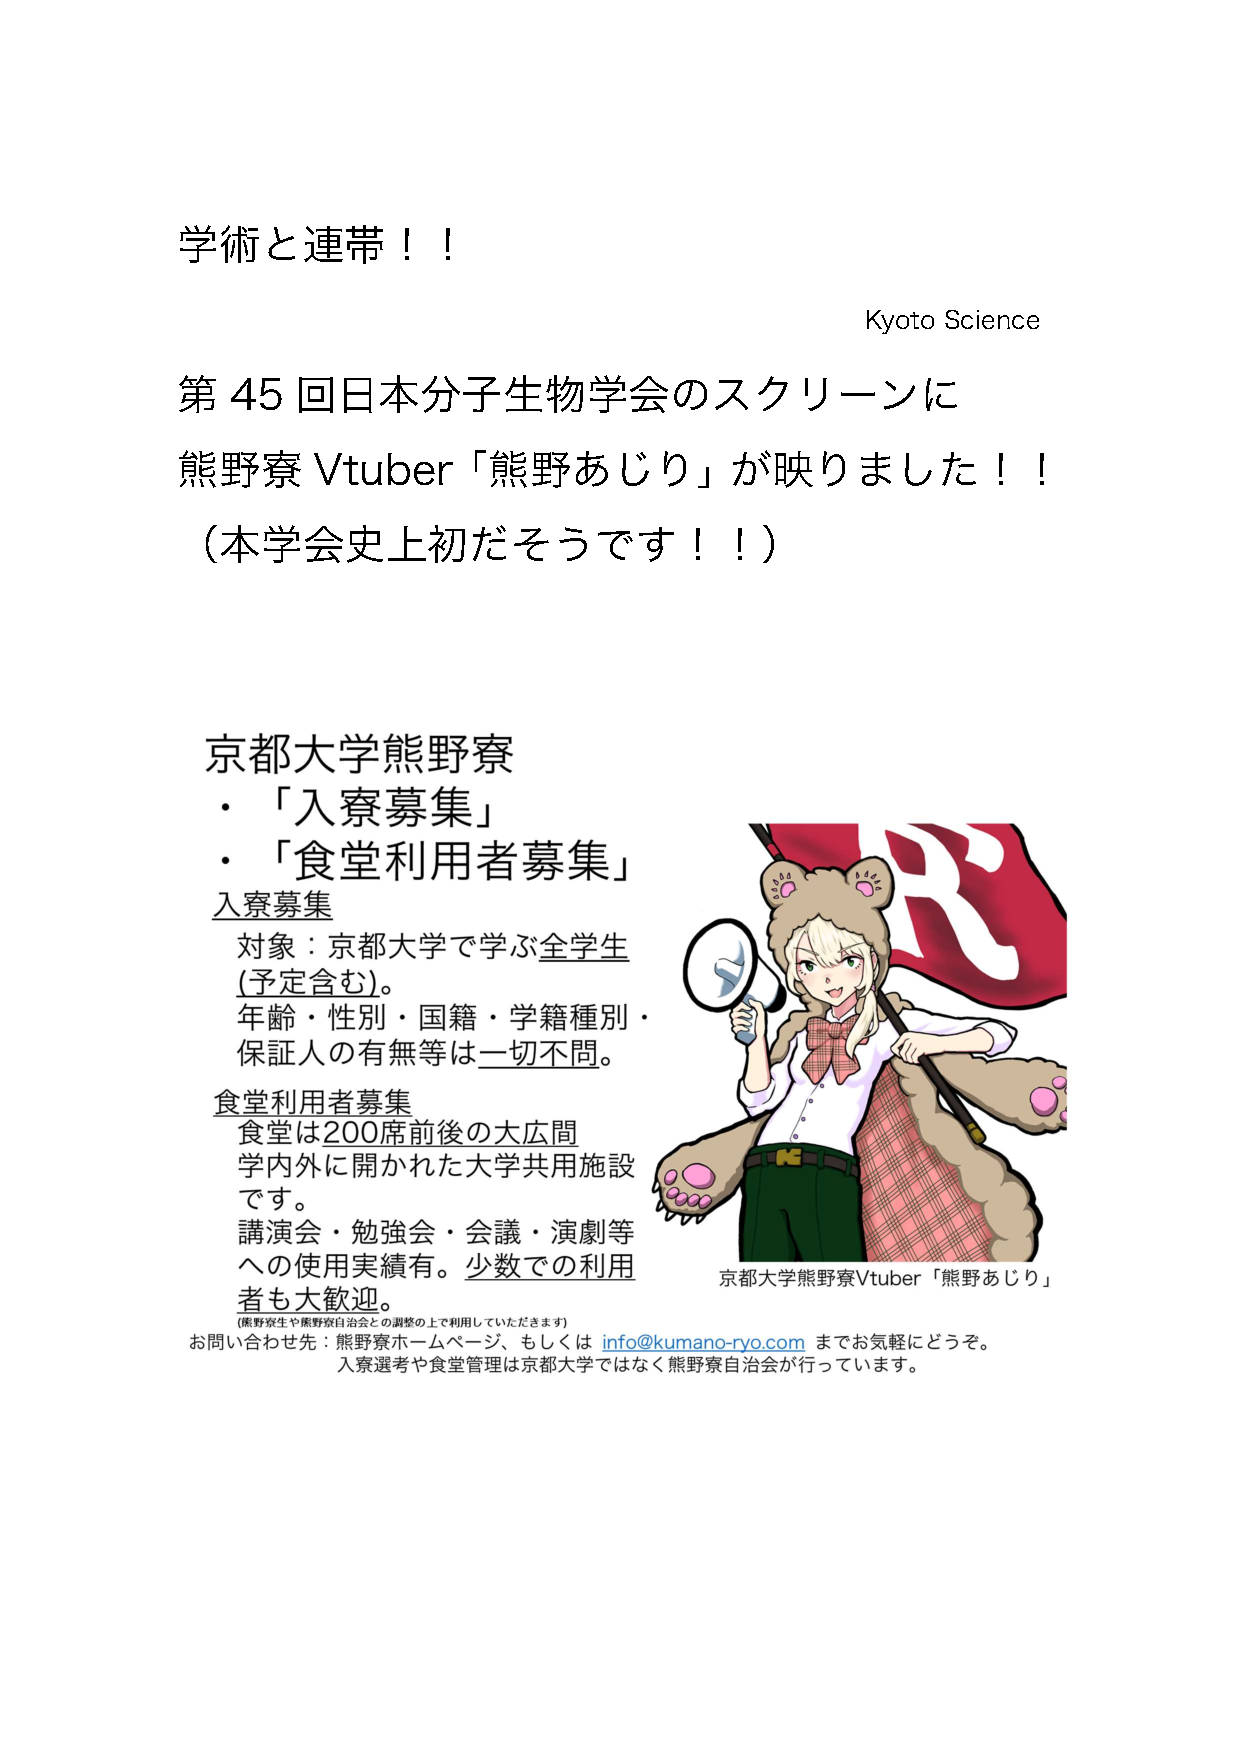
\includegraphics[width=\textwidth]{gazo/gakujututo1.pdf}
\end{figure}

\newpage

\begin{figure}[H]
  \centering
  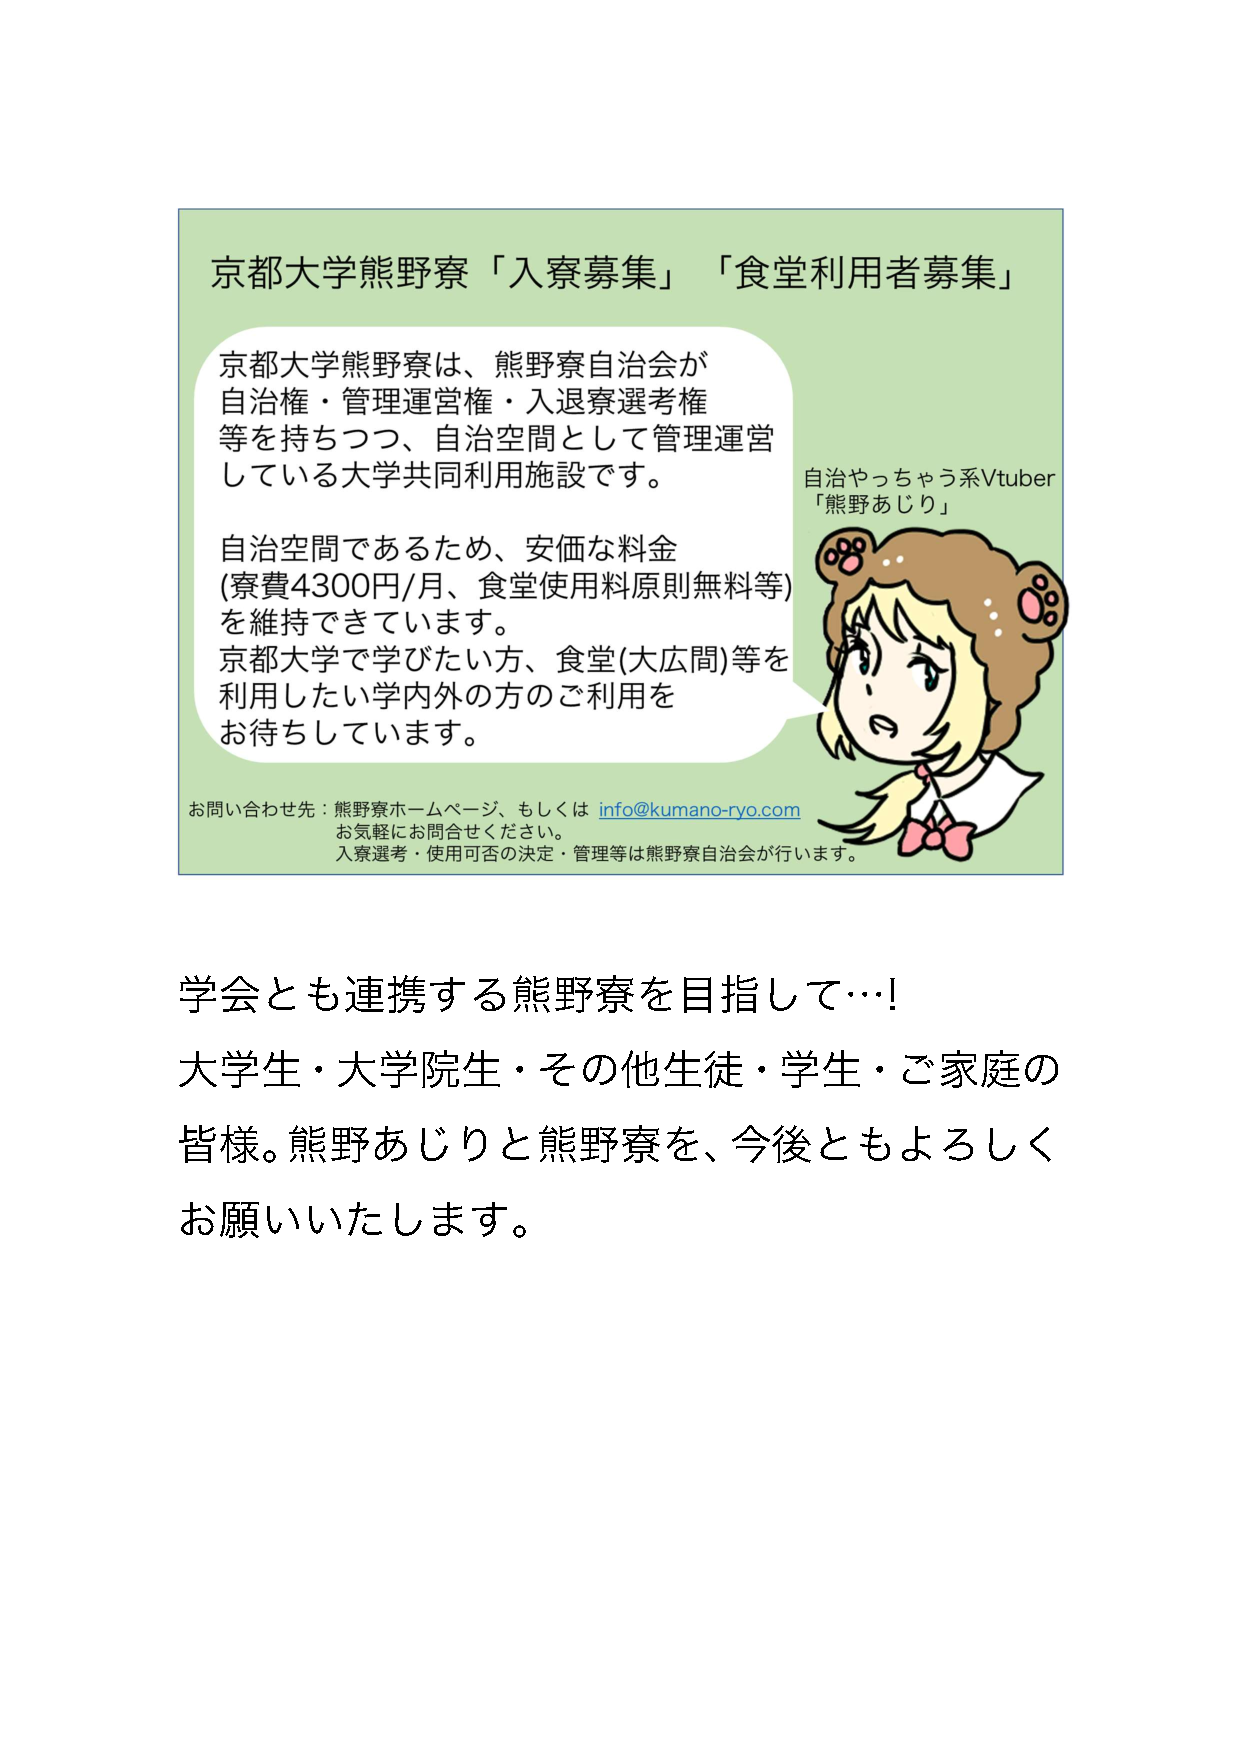
\includegraphics[width=\textwidth]{gazo/gakujututo2.pdf}
\end{figure}

  

  \input{memo.tex}
  %\input{memo.tex}

  \input{memo.tex}
  \printindex
  
  
% 奥付
% 下寄せ
\vspace*{\fill} % *をつけるとページ先頭でも入る。


\begin{flushleft}
  % 幅いっぱいにするためにtabular*環境を使用
  % @{}とするとパディングがなくなる
  % また、@{...}とすると、セルの区切りに...が入る
  \begin{tabular*}{\textwidth}{@{}l@{\extracolsep{\fill}}}
      \textbf{\huge 京都大学熊野寮入寮パンフレット2023} \\
      \hline
      \begin{tabular}{@{}r@{年\kern.5zw}r@{月\kern.5zw}r@{日\kern1.5zw}ll}
          2023 &  2 & 25 & 発行 & \\
      \end{tabular} \\
      \\
      \begin{tabular}{@{}l@{\kern.5zw\textbf{:}\kern1zw}l}
          \textbf{編者} & 京都大学熊野寮自治会 \\
          \textbf{発行} & 京都大学熊野寮自治会 \\
          \textbf{印刷} & 京都大学熊野寮 \\
      \end{tabular} \\
      \hline
  \end{tabular*}
\end{flushleft}

  



\end{document}